% Options for packages loaded elsewhere
\PassOptionsToPackage{unicode}{hyperref}
\PassOptionsToPackage{hyphens}{url}
%
\documentclass[
]{book}
\usepackage{lmodern}
\usepackage{amssymb,amsmath}
\usepackage{ifxetex,ifluatex}
\ifnum 0\ifxetex 1\fi\ifluatex 1\fi=0 % if pdftex
  \usepackage[T1]{fontenc}
  \usepackage[utf8]{inputenc}
  \usepackage{textcomp} % provide euro and other symbols
\else % if luatex or xetex
  \usepackage{unicode-math}
  \defaultfontfeatures{Scale=MatchLowercase}
  \defaultfontfeatures[\rmfamily]{Ligatures=TeX,Scale=1}
\fi
% Use upquote if available, for straight quotes in verbatim environments
\IfFileExists{upquote.sty}{\usepackage{upquote}}{}
\IfFileExists{microtype.sty}{% use microtype if available
  \usepackage[]{microtype}
  \UseMicrotypeSet[protrusion]{basicmath} % disable protrusion for tt fonts
}{}
\makeatletter
\@ifundefined{KOMAClassName}{% if non-KOMA class
  \IfFileExists{parskip.sty}{%
    \usepackage{parskip}
  }{% else
    \setlength{\parindent}{0pt}
    \setlength{\parskip}{6pt plus 2pt minus 1pt}}
}{% if KOMA class
  \KOMAoptions{parskip=half}}
\makeatother
\usepackage{xcolor}
\IfFileExists{xurl.sty}{\usepackage{xurl}}{} % add URL line breaks if available
\IfFileExists{bookmark.sty}{\usepackage{bookmark}}{\usepackage{hyperref}}
\hypersetup{
  pdftitle={Complex-valued Econometrics with Examples in R},
  pdfauthor={Sergey Svetunkov and Ivan Svetunkov},
  hidelinks,
  pdfcreator={LaTeX via pandoc}}
\urlstyle{same} % disable monospaced font for URLs
\usepackage{color}
\usepackage{fancyvrb}
\newcommand{\VerbBar}{|}
\newcommand{\VERB}{\Verb[commandchars=\\\{\}]}
\DefineVerbatimEnvironment{Highlighting}{Verbatim}{commandchars=\\\{\}}
% Add ',fontsize=\small' for more characters per line
\usepackage{framed}
\definecolor{shadecolor}{RGB}{248,248,248}
\newenvironment{Shaded}{\begin{snugshade}}{\end{snugshade}}
\newcommand{\AlertTok}[1]{\textcolor[rgb]{0.94,0.16,0.16}{#1}}
\newcommand{\AnnotationTok}[1]{\textcolor[rgb]{0.56,0.35,0.01}{\textbf{\textit{#1}}}}
\newcommand{\AttributeTok}[1]{\textcolor[rgb]{0.77,0.63,0.00}{#1}}
\newcommand{\BaseNTok}[1]{\textcolor[rgb]{0.00,0.00,0.81}{#1}}
\newcommand{\BuiltInTok}[1]{#1}
\newcommand{\CharTok}[1]{\textcolor[rgb]{0.31,0.60,0.02}{#1}}
\newcommand{\CommentTok}[1]{\textcolor[rgb]{0.56,0.35,0.01}{\textit{#1}}}
\newcommand{\CommentVarTok}[1]{\textcolor[rgb]{0.56,0.35,0.01}{\textbf{\textit{#1}}}}
\newcommand{\ConstantTok}[1]{\textcolor[rgb]{0.00,0.00,0.00}{#1}}
\newcommand{\ControlFlowTok}[1]{\textcolor[rgb]{0.13,0.29,0.53}{\textbf{#1}}}
\newcommand{\DataTypeTok}[1]{\textcolor[rgb]{0.13,0.29,0.53}{#1}}
\newcommand{\DecValTok}[1]{\textcolor[rgb]{0.00,0.00,0.81}{#1}}
\newcommand{\DocumentationTok}[1]{\textcolor[rgb]{0.56,0.35,0.01}{\textbf{\textit{#1}}}}
\newcommand{\ErrorTok}[1]{\textcolor[rgb]{0.64,0.00,0.00}{\textbf{#1}}}
\newcommand{\ExtensionTok}[1]{#1}
\newcommand{\FloatTok}[1]{\textcolor[rgb]{0.00,0.00,0.81}{#1}}
\newcommand{\FunctionTok}[1]{\textcolor[rgb]{0.00,0.00,0.00}{#1}}
\newcommand{\ImportTok}[1]{#1}
\newcommand{\InformationTok}[1]{\textcolor[rgb]{0.56,0.35,0.01}{\textbf{\textit{#1}}}}
\newcommand{\KeywordTok}[1]{\textcolor[rgb]{0.13,0.29,0.53}{\textbf{#1}}}
\newcommand{\NormalTok}[1]{#1}
\newcommand{\OperatorTok}[1]{\textcolor[rgb]{0.81,0.36,0.00}{\textbf{#1}}}
\newcommand{\OtherTok}[1]{\textcolor[rgb]{0.56,0.35,0.01}{#1}}
\newcommand{\PreprocessorTok}[1]{\textcolor[rgb]{0.56,0.35,0.01}{\textit{#1}}}
\newcommand{\RegionMarkerTok}[1]{#1}
\newcommand{\SpecialCharTok}[1]{\textcolor[rgb]{0.00,0.00,0.00}{#1}}
\newcommand{\SpecialStringTok}[1]{\textcolor[rgb]{0.31,0.60,0.02}{#1}}
\newcommand{\StringTok}[1]{\textcolor[rgb]{0.31,0.60,0.02}{#1}}
\newcommand{\VariableTok}[1]{\textcolor[rgb]{0.00,0.00,0.00}{#1}}
\newcommand{\VerbatimStringTok}[1]{\textcolor[rgb]{0.31,0.60,0.02}{#1}}
\newcommand{\WarningTok}[1]{\textcolor[rgb]{0.56,0.35,0.01}{\textbf{\textit{#1}}}}
\usepackage{longtable,booktabs}
% Correct order of tables after \paragraph or \subparagraph
\usepackage{etoolbox}
\makeatletter
\patchcmd\longtable{\par}{\if@noskipsec\mbox{}\fi\par}{}{}
\makeatother
% Allow footnotes in longtable head/foot
\IfFileExists{footnotehyper.sty}{\usepackage{footnotehyper}}{\usepackage{footnote}}
\makesavenoteenv{longtable}
\usepackage{graphicx}
\makeatletter
\def\maxwidth{\ifdim\Gin@nat@width>\linewidth\linewidth\else\Gin@nat@width\fi}
\def\maxheight{\ifdim\Gin@nat@height>\textheight\textheight\else\Gin@nat@height\fi}
\makeatother
% Scale images if necessary, so that they will not overflow the page
% margins by default, and it is still possible to overwrite the defaults
% using explicit options in \includegraphics[width, height, ...]{}
\setkeys{Gin}{width=\maxwidth,height=\maxheight,keepaspectratio}
% Set default figure placement to htbp
\makeatletter
\def\fps@figure{htbp}
\makeatother
\setlength{\emergencystretch}{3em} % prevent overfull lines
\providecommand{\tightlist}{%
  \setlength{\itemsep}{0pt}\setlength{\parskip}{0pt}}
\setcounter{secnumdepth}{5}
\usepackage{booktabs}
\usepackage{amsthm, graphicx, amssymb, amsmath}
\makeatletter
\def\thm@space@setup{%
  \thm@preskip=8pt plus 2pt minus 4pt
  \thm@postskip=\thm@preskip
}
\makeatother

\newtheorem*{adamCitation}{Citation}
\newtheorem*{remark}{Remark}
\newtheorem*{definition}{Definition}
\newtheorem*{task}{Task}
\newtheorem*{solution}{Solution}
\DeclareMathOperator\Arg{Arg}
\usepackage{booktabs}
\usepackage{longtable}
\usepackage{array}
\usepackage{multirow}
\usepackage{wrapfig}
\usepackage{float}
\usepackage{colortbl}
\usepackage{pdflscape}
\usepackage{tabu}
\usepackage{threeparttable}
\usepackage{threeparttablex}
\usepackage[normalem]{ulem}
\usepackage{makecell}
\usepackage{xcolor}
\usepackage[]{natbib}
\bibliographystyle{elsarticle-harv}

\title{Complex-valued Econometrics with Examples in R}
\author{Sergey Svetunkov and Ivan Svetunkov}
\date{2024-01-31}

\begin{document}
\maketitle

{
\setcounter{tocdepth}{2}
\tableofcontents
}
\hypertarget{introduction}{%
\chapter*{Introduction}\label{introduction}}
\addcontentsline{toc}{chapter}{Introduction}

The theory of complex variables functions is actively used in a variety of disciplines, including modern physics and engineering sciences. It is relatively easy to describe the complex phenomena that are studied in these areas of science using the models and methods of this branch of mathematics. Social sciences, being much more complicated due to the unpredictability of human behaviour, tend to use simpler instruments for modelling complex processes (references). For example, there are only few scientific publications in which methods and models of the theory of complex variables functions are used in economics, and they typically use that instrument for diagnostics or statistical tests (references) rather than proper modelling.

In 2012, Springer published the monograph ``Complex-valued Modeling in Economics and Finance'' \citep{Svetunkov2012}, which presented the theory and methodology of modelling using complex variables in economics. \citet{Svetunkov2012} have summarised the main principles of using complex variables in economics and discussed how to estimate some of those models. While, this was the first monograph that discussed the topic, the first paper in this direction was Ben Tamari (1997). The author first introduced Wealth as a complex variable consisting of Output (real part) and Money (imaginary part) and showed how, even with such an elementary representation, interesting new results can be obtained in the area of economics. Unfortunately, this work has gone unnoticed in scientific world. We became aware of this work only in 2016, when Ben Tamari had kindly sent Sergey Svetunkov his paper.

Since 2012, there has been some development in the area of modelling using complex variables, notably a paper by Svetunkov \& Kourentzes (2022) on Complex Exponential Smoothing and Kourentez et al.~(2019) on an error measure based on the idea of complex numbers. Up until now, the modelling with complex variables has been mainly picked up by academics working in the areas of forecasting and engineering. The latter group has been using complex autoregressions for a couple of decades, modelling and predicting signals. The former group has only started using the principles described in \citet{Svetunkov2012}. In other disciplines, complex variables are not used directly for model building. The probable reason for this is the lack of the communication between the disciplines and the inherited inertia of academia.

In a try to speed up the adoption of the new instrument, we have written this monograph, summarising the research that has been done in the area of dynamic models since 2012. We should clarify that the term ``dynamic model'' used in this monograph refers to models that have a structure that changes over time. The classical example of such a model is ARIMA (AutoRegression Integrated with Moving Average by Box \& Jenkins, 1976), which allows producing forecasts for a variety of processes based on the existing historical time series. Another example is a multivariate version of ARMA, Vector ARMA or VARMA, which allows modelling the dynamics of several related processes simultaneously. For instance, in business and economics, these models are used for prices, demand forecasting and for capturing complex interactions between macroeconomic indicators over time.
However, all autoregression models that exist today use real variables. In this monograph we will discuss their complex-valued counterparts, namely complex ARIMA and complex VARMA, and study their properties, showing how to identify their orders and how to estimate these models in practice. But before rushing into the discussion, we will explain the basics of random complex variables and complex-valued statistics, which has been developed in signal processing literature, but has not been used to its full potential.

Chapter 1 discusses the theory of random complex variables, conventional and complex-valued statistics, the complex least squares method, maximum likelihood and complex autocorrelation and partial autocorrelation functions. In Chapter 2, we will move to the discussion of simple dynamic model -- complex AR, starting from its properties and slowly moving to its identification and estimation and then to forecasting. After that, in Chapter 3, we will move towards complex MA, again discussing its properties and how one can apply it in practice. The two parts will be united in a cARIMA model in Chapter 4, where we will also discuss seasonal counterpart of the model. Finally, we will move to vector models in Chapter 5, introducing cVAR, cVMA and cVARMA, showing their advantages in comparison with the conventional real valued models. All of this will be supported by examples in R, which will rely heavily on the package ``complex'', developed especially for this monograph. This means that anyone can then use the proposed models for purposes of time series analysis and forecasting.

This work was partially supported by the Russian Foundation for Basic Research (grant No.~19-010-00610\textbackslash19 ``Theory, methods and methodologies of forecasting economic development by autoregression models of complex variables''). Thanks to this support, it became possible to carry out this research in general, forming a new scientific direction in statistical modelling and short-term forecasting.

The authors are grateful to those young scientists of St.~Petersburg Polytechnic University of Peter the Great, who participated in this study, patiently testing the author's hypotheses. They helped forming the theory behind the models discussed in this monograph. We are pleased to mention their names: Evgeny Goltsev, Nikolai Pitukhin, Victoria Matskevich, Yulia Selivanova, Galina Siruk and Nazira Shaikhleeva.

This monograph relies heavily on the \texttt{complex} package for R. Many of the examples in R will use functions from this package, so make sure to install it before running any R code \citep{R-complex}:

\begin{Shaded}
\begin{Highlighting}[]
\KeywordTok{install.packages}\NormalTok{(}\StringTok{"complex"}\NormalTok{)}
\end{Highlighting}
\end{Shaded}

We will also need several other packages for our analysis, including the following:

\begin{Shaded}
\begin{Highlighting}[]
\KeywordTok{library}\NormalTok{(mvtnorm)}
\KeywordTok{library}\NormalTok{(tseries)}
\KeywordTok{library}\NormalTok{(greybox)}
\end{Highlighting}
\end{Shaded}

\hypertarget{who-is-this-monograph-for}{%
\section*{Who is this monograph for?}\label{who-is-this-monograph-for}}
\addcontentsline{toc}{section}{Who is this monograph for?}

\hypertarget{intro}{%
\chapter{Introduction to theory of complex variables}\label{intro}}

\hypertarget{theoryOfComplexNumbers}{%
\section{Theory of complex numbers}\label{theoryOfComplexNumbers}}

This section sets out the basic concepts of the Theory of Complex Variables Functions (TCVF) with some historical overlook of the idea of complex numbers. Hopefully, this will help in understanding the main idea that we will use extensively in the following chapters.

The theory of complex numbers started in 1572 in the small Italian town of Kura. It was in this place and precisely in this year that the manuscript of an Italian mathematician Rafael Bombelli was published. The book was called Algebra. Rafael Bombelli showed in it how to solve the following cubic equation:
\begin{equation}
    x^3 = 15x + 4 .
    \label{eq:BombelliEquation}
\end{equation}
The root of cubic equations at that time was calculated using the formula of Scipione del Ferro. With regards to the task at hand, finding the root should have been carried out as follows:
\begin{equation}
    \begin{aligned}
    x = & \sqrt[3]{\frac{4}{2}+\sqrt{\left(\frac{4}{2}\right)^2 - \left(\frac{15}{3}\right)^3}} + \sqrt[3]{\frac{4}{2}-\sqrt{\left(\frac{4}{2}\right)^2 - \left(\frac{15}{3}\right)^3}} = \\
        & \sqrt[3]{2+\sqrt{-121}} + \sqrt[3]{2-\sqrt{-121}} .
    \end{aligned}
    \label{eq:BombelliSolution}
\end{equation}
As can be seen from equation \eqref{eq:BombelliSolution}, there are several square roots, and it follows directly from the right hand side of this equation that to calculate the roots of equation \eqref{eq:BombelliEquation}, we need to extract the square root from the negative number, -121. This means that it will not be possible to find a solution to this equation in the domain of real numbers.

This does not mean that equation \eqref{eq:BombelliEquation} does not have a solution. If you represent the problem graphically on a plane then it is easy to see that there is one. But it is impossible to find it arithmetically using the Scipione del Ferro formula, because there is a negative number in the expression on the right-hand side of \eqref{eq:BombelliSolution}, and back then, mathematicians were sure that the square root of a negative number does not exist.

The mathematicians of that time struggled to solve this problem, and Rafael Bombelli suggested to ignore the negative sign in the expression (Bombelli, 12). After all, the number -121 can be represented as a product of two numbers: -1 and 121. Then the square root of this number can be written as \(\sqrt{-1} \times 11\). So, formula \eqref{eq:BombelliSolution} becomes:
\begin{equation}
    x = \sqrt[3]{2+11\sqrt{-1}} + \sqrt[3]{2-11\sqrt{-1}} .
    \label{eq:BombelliSolutionSqrt}
\end{equation}
Now it is possible to get a solution of the problem, and the root of the cubic equation is \(x = 4\).

For a long time, Bombelli's approach was considered by scientists as a convenient mathematical trick. And the square root of minus one was called ``magic unit'', ``vanishing unit'', etc. Finally, the term ``imaginary unit'' was established by René Descartes in 1637 and any number multiplied by the imaginary unit would be called ``imaginary number''. Merging a real number with an imaginary number gives another number, which can be considered as a more general to the two, which is called ``complex''. It can be written as:
\begin{equation}
    \underline{z} = x+iy ,
    \label{eq:complexNumber}
\end{equation}
where \(x\) is the real part, \(iy\) is the imaginary part of a complex number, \(x\) and \(y\) are real numbers and \(i\) is the imaginary unit that satisfies the equality:
\begin{equation}
    i^2 = -1 .
    \label{eq:imaginaryUnit}
\end{equation}
We use the symbol \(\underline{}\) to denote a complex number.

With complex numbers, one can perform almost all the same operations as with the real ones. However, taking into account the properties of the imaginary unit, these operations can lead to results that are not common in the domain of real numbers.

The main problem that analysts face when trying to understand a complex number is the complexity of the interpretation of the imaginary part. The main question in this case can be formulated as: Where do imaginary numbers appear in practice? And what is the practical meaning of an imaginary unit? We have heard questions like that many times, and while they are valid, we think that they do not have appropriate answers and divert the analysts from what the modelling with complex variables brings.

We argue that the imaginary unit does not have any practical meaning: neither in economics, nor in sociology, nor in engineering, nor in physics. The imaginary unit is a mathematical rule, and that is all. It is a mathematical abstract that has useful properties. A number \(\sqrt{2}\) or \(\ln 3\) do not have practical meaning either, but they are useful for modelling purposes and solving applied problems in a variety of disciplines. Similarly, an imaginary unit is convenient for solving a whole class of problems in different areas of application. With the help of the rules specified by conditions \eqref{eq:complexNumber} and \eqref{eq:imaginaryUnit}, it is possible to use new mathematical operations, obtain new mathematical results, and create new mathematical models.

Imaginary and complex numbers are mathematical instruments that can help in describing a real-life phenomenon. If a researcher decides to use complex variables for real processes modelling, they will need to predefine the rules according to which one component of a complex process is attributed to the real part, and another one is attributed to the imaginary part of the complex variable. These rules might seem arbitrary, because there is no ``true'' recipe, according to which the assignment to complex variable parts should be done. The main motivation for them is the efficiency of modelling (such as goodness of fit or forecasting accuracy) and nothing else.

In order to better understand how the modelling with complex variables can be done, we need to better understand how complex variables can be represented and interpreted. A real number represents visually a certain segment on the numerical axis, which has a zero point and a multitude of values from minus infinity to infinity. Any real number is characterized by the distance from zero to the value of that number. Negative numbers are located to the left of zero, while the positive ones are located to the right of it.

A complex number consists of two parts, which can be visualised on the plane with two perpendicular axes, where the real numbers are marked on the horizontal line, and the imaginary ones are on the vertical one. This is shown visually in Figure \ref{fig:complexPlane} with a complex number \(\underline{z}=x+iy\).

\begin{figure}
\centering
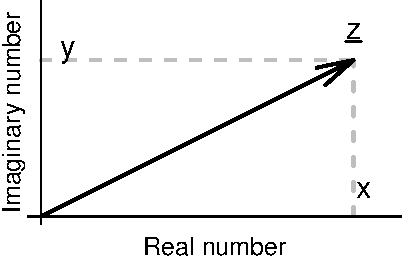
\includegraphics{Svetunkov---Svetunkov---Complex-Valued-Econometrics_files/figure-latex/complexPlane-1.pdf}
\caption{\label{fig:complexPlane}Visual presentation of a complex number on the complex plane.}
\end{figure}

Any point lying on the complex plane in Figure \ref{fig:complexPlane} characterises a complex number, even if that point lies on the axis of real numbers. In that specific case, we would be talking about a complex number with a zero imaginary part, i.e.~\(\underline{z}=x+i0\).

Given that complex numbers can be represented on a plane (in so called Cartesian coordinates), the number \eqref{eq:complexNumber} can be represented in a form of a vector that starts in the origin of coordinates and ends at the point (x, y). Then any complex number can be represented in form of polar coordinates using the magnitude of the vector and its polar angle:
\begin{equation}
    \underline{z} = x+iy = r (\cos \phi + i \sin \phi),
    \label{eq:complexNumberTrigonometric}
\end{equation}
where \(r=|\underline{z}|\) is the magnitude, which is calculated as a Euclidean distance from the origin to the point (x, y) on the plane:
\begin{equation}
    r = \sqrt{x^2 + y^2},
    \label{eq:complexNumberMagnitude}
\end{equation}
and \(\phi=\Arg(\underline{z})\) is the angle, which equals to:
\begin{equation}
    \phi = \arctan \frac{y}{x} + 2 \pi l,
    \label{eq:complexNumberAngle}
\end{equation}
where \(l\) is an integer number. While depending on a task, \(l\) can be set to a positive, a negative number, or a zero, for convenience, we will restrict it to \(l=0\), because all the other values will not be useful for the inference in following chapters. The polar angle is sometimes referred to as the argument of a complex number.

Using the magnitude and the polar angle, we can also represent any complex number in the exponential form, which was first proposed in 1748 by Euler, in his book ``Introduction to the Infinitesimal Analysis'' \textbf{(Euler, 1961, pp.~118-119)}, which:
\begin{equation}
    \underline{z} = r e^{i \phi} ,
    \label{eq:complexNumberExponential}
\end{equation}
where \(e\) is the Euler's constant. Equation \eqref{eq:complexNumberExponential} is nowadays also called ``Euler's form''. Comparing @ref\{eq:complexNumberTrigonometric\} with @ref\{eq:complexNumberExponential\}, we can conclude that:
\begin{equation}
    e^{i \phi} = \cos \phi + i \sin \phi ,
    \label{eq:EulerFormula}
\end{equation}
which gives the connection between the linear, trigonometric and exponential forms of a complex number. In the exponential form \eqref{eq:complexNumberExponential}, a positive real number has \(\phi=0\), while a negative one has \(\phi=\pi\), and all imaginary numbers have an angle dividable by \(\frac{\pi}{2}\). So, for example:
\begin{equation*}
    \begin{aligned}
    41 = & 41 e^{i 0} \\
    i41 = & 41 e^{i \frac{\pi}{2}} \\
    -41 = & 41 e^{i \pi} \\
    -i41 = & 41 e^{i \frac{3 \pi}{2}}
    \end{aligned}
\end{equation*}
In fact, multiplication of any complex number by the imaginary unit implies the rotation of complex vector by \(\frac{\pi}{2}\), as shown in Figure \ref{fig:complexPlaneMultiplication}, where a complex number \(\underline{z}_1 = x_1 + i y_1\) becomes \(\underline{z}_2 = \underline{z}_1 \times i = x_2 + i y_2\) etc.

\begin{figure}
\centering
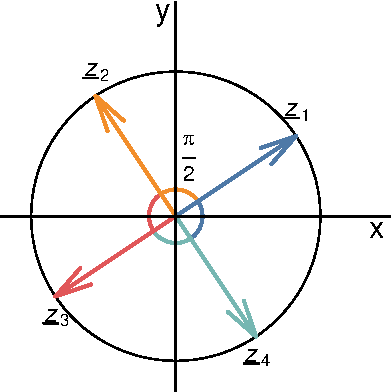
\includegraphics{Svetunkov---Svetunkov---Complex-Valued-Econometrics_files/figure-latex/complexPlaneMultiplication-1.pdf}
\caption{\label{fig:complexPlaneMultiplication}Multiplication of a complex number by \(i\) implies the rotation of it by \(\frac{\pi}{2}\).}
\end{figure}

In a way, any mathematical operation with a complex number implies a change in magnitude and angle of the number, while the multiplication and division by a number with non-zero imaginary part will always lead to the rotation of the vector. Operations of addition and subtraction are simpler in the linear form:
\begin{equation*}
    \underline{z}_3 = \underline{z}_1 + \underline{z}_2 = x_1 + x_2 + i (y_1 + y_2) ,
\end{equation*}
while operations of multiplication and division are easier to do in either exponential or trigonometric forms of complex numbers:
\begin{equation*}
    \underline{z}_3 = \underline{z}_1 \times \underline{z}_2 = r_1 r_2 e^{i \phi_1 + \phi_2} 
\end{equation*}
or:
\begin{equation*}
    \underline{z}_3 = r_1 r_2 \left(\cos (\phi_1 + \phi_2) + i \sin (\phi_1 + \phi_2) \right) .
\end{equation*}

Furthermore, given that any complex number can be represented in the exponential form \eqref{eq:complexNumberExponential}, it can also be visualised on a polar coordinates plane, where the magnitude is marked on the x-axis, and the polar angle is marked on the y-axis. This is shown visually in Figure \ref{fig:complexPlanePolar}.

\begin{figure}
\centering
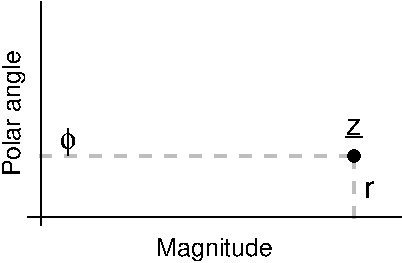
\includegraphics{Svetunkov---Svetunkov---Complex-Valued-Econometrics_files/figure-latex/complexPlanePolar-1.pdf}
\caption{\label{fig:complexPlanePolar}Visual presentation of a complex number in the polar coordinates.}
\end{figure}

The usefulness of the polar coordinates presentation becomes apparent when a set of complex numbers is considered, because then in some cases it becomes possible to see some relations that are not obvious on the Cartesian plane. Figure \ref{fig:complexCartesianvsPolar} shows an example of a set of complex random numbers, for which the real and imaginary parts do not seem to have any obvious linear relation, but the magnitude and the angle have a negative relation.

\begin{figure}
\centering
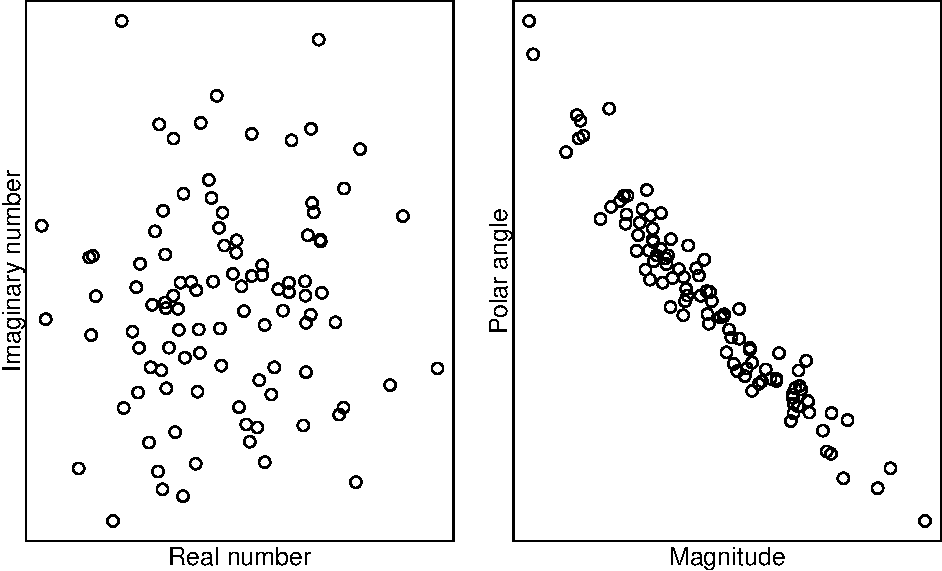
\includegraphics{Svetunkov---Svetunkov---Complex-Valued-Econometrics_files/figure-latex/complexCartesianvsPolar-1.pdf}
\caption{\label{fig:complexCartesianvsPolar}Visualisation of a set of complex numbers on Cartesian and on polar coordinates planes.}
\end{figure}

In this case, modelling can be done in the exponential form of complex numbers, which might allow capturing complicated non-linear relations between variables.

When it comes to comparing complex numbers, mathematically we will say that two complex numbers \(\underline{z}_1 = x_1 + i y_1\) and \(\underline{z}_2 = x_2 + i y_2\) are equal to each other if and only if their real and imaginary parts are equal:
\begin{equation*}
    \underline{z}_1 = \underline{z}_2 \iff \left \lbrace
    \begin{aligned}
        & x_1 = x_2 \\
        & y_1 = y_2
    \end{aligned}
    \right. ,
\end{equation*}
which is equivalent to saying that their magnitudes and polar angles are equal:
\begin{equation*}
    \underline{z}_1 = \underline{z}_2 \iff \left \lbrace
    \begin{aligned}
        & |\underline{z}_1| = |\underline{z}_2| \\
        & \Arg(\underline{z}_1) = \Arg(\underline{z}_2)
    \end{aligned}
    \right. .
\end{equation*}

Unfortunately, given that complex numbers are two dimensional, it is not possible to say in general whether one number is greater or less than the other. However, we could use magnitude to compare complex numbers, to say which one lies further away from the origin than the other. In that case, the number with a larger magnitude could be considered as a greater than the one with the smaller magnitude. While we could compare the polar angles as well, they only give us information about rotation of a complex number and thus do not give any meaningful information about the comparison of numbers. So, two complex numbers in Figure \ref{fig:complexPlaneCircle} would have the same magnitude, but will have different angles, and it is not possible to say whether one number is greater than the other in this case. In order to conclude that, we would need to devise additional criteria for comparison of numbers (e.g.~positive numbers are ``better'' than the negative ones, thus \(\phi_1=\pi\) and \(\phi_1=-\pi\) is ``worse'' than \(\phi_2=0\)).

\begin{figure}
\centering
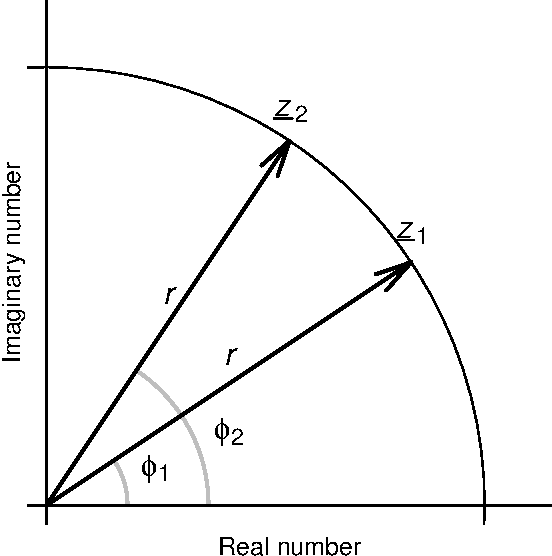
\includegraphics{Svetunkov---Svetunkov---Complex-Valued-Econometrics_files/figure-latex/complexPlaneCircle-1.pdf}
\caption{\label{fig:complexPlaneCircle}Comparison of two complex numbers \(\underline{z}_1\) and \(\underline{z}_2\) that have the same magnitude \(r\), but different angles \(\phi_1\) and \(\phi_2\).}
\end{figure}

Continuing the discussion of different forms of a complex number, its magnitude can be represented in exponential form:
\begin{equation*}
    r = e^{\ln(r)},
\end{equation*}
where \(\ln\) is the natural logarithm. This can then be used to rewrite the exponential form of a complex number as:
\begin{equation}
    \underline{z} = e^{\ln r + i \phi} ,
    \label{eq:complexNumberExponentialAll}
\end{equation}
And this form allows calculating logarithms of a complex number:
\begin{equation}
    \ln \underline{z} = \ln \left(e^{\ln r + i \phi} \right) = \ln r + i \phi .
    \label{eq:complexNumberLogarithm}
\end{equation}
This operation will become useful when we discuss transformations of complex-valued functions, but it also shows that a logarithm of a negative real number is a complex number, because in that case \(\phi=\pi\). This demonstrates that the field of complex numbers is complete: any mathematical operation of a complex number will give another complex number.

One of the important definitions in theory of complex numbers is the conjugate complex number. It is the number, for which the imaginary part has the sign opposite to the one of the original variable. For example, the conjugate of the complex variable \(\underline{z} = x+ iy\) is \(\underline{\tilde{z}} = x- iy\). These numbers are useful because the multiplication of a complex number by its conjugate gives a real number:
\begin{equation}
    \underline{z} \times \underline{\tilde{z}} = (x+ iy) (x- iy) = x^2 + y^2 ,
    \label{eq:complexNumberConjugateMulti}
\end{equation}
which is the square of the magnitude \eqref{eq:complexNumberMagnitude} of both complex variables \(\underline{z}\) and \(\underline{\tilde{z}}\). Conjugation is distributive over addition, subtraction, multiplication and division, meaning that:
\begin{equation}
    \begin{aligned}
        & \widetilde{x + y} = \tilde{x} + \tilde{y} \\
        & \widetilde{x - y} = \tilde{x} - \tilde{y} \\
        & \widetilde{x \times y} = \tilde{x} \times \tilde{y} \\
        & \widetilde{\left(\frac{x}{y}\right)} = \frac{\tilde{x}}{\tilde{y}} .
    \end{aligned}
    \label{eq:complexNumberConjugateDistributive}
\end{equation}

Finally, given that any complex number can be represented visually in a form of a vector, we can write it mathematically either like vector:
\begin{equation}
    \boldsymbol{z} = \begin{pmatrix} x \\ y \end{pmatrix}
    \label{eq:complexNumberVectors}
\end{equation}
or like a matrix:
\begin{equation}
    \underset{\sim}{\boldsymbol{z}} = \begin{pmatrix} x & -y \\ y & x \end{pmatrix} ,
    \label{eq:complexNumberMatrix}
\end{equation}
where the symbold \(\sim\) below the letter denotes a matrix presentation of a complex number. In the matrix notation, any real number can be represented as a diagonal matrix, while any imaginary one is a matrix with zero diagonal:
\begin{equation*}
    \begin{aligned}
        & \begin{pmatrix} x & 0 \\ 0 & x \end{pmatrix} \\
        & \begin{pmatrix} 0 & -y \\ y & 0 \end{pmatrix}
    \end{aligned} .
\end{equation*}
All the mathematical operations done with the vector and matrix representations would correspond to the ones for the conventional complex numbers. Furthermore, the multiplication by the transpose of the original object in both of these cases is equivalent to the multiplication by the conjugate value \eqref{eq:complexNumberConjugateMulti}. For the vector:
\begin{equation}
    \boldsymbol{z} \boldsymbol{z}^\prime = \begin{pmatrix} x & y \end{pmatrix} \times \begin{pmatrix} x \\ y \end{pmatrix} = \begin{pmatrix} x^2 + y^2 \end{pmatrix}
    \label{eq:complexNumberVectorsMulti}
\end{equation}
and for the matrix:
\begin{equation}
    \underset{\sim}{\boldsymbol{z}} \underset{\sim}{\boldsymbol{z}}^\prime = \begin{pmatrix} x & -y \\ y & x \end{pmatrix} \times \begin{pmatrix} x & y \\ -y & x \end{pmatrix} = 
    \begin{pmatrix} x^2 + y^2 & 0 \\ 0 & x^2 + y^2 \end{pmatrix}.
    \label{eq:complexNumberMatrixMulti}
\end{equation}
These transpositions will be called in this monograph ``conjugate transpositions''. The vector and matrix representations become especially useful when we work with complex variables to construct complex models. Finally, in case of matrix form, it is possible to multiply complex variable by itself without the conjugation, which results in:
\begin{equation}
    \underset{\sim}{\boldsymbol{z}} \underset{\sim}{\boldsymbol{z}}^{\top} = \begin{pmatrix} x & -y \\ y & x \end{pmatrix} \times \begin{pmatrix} x & -y \\ y & x \end{pmatrix} = 
    \begin{pmatrix} x^2 - y^2 & - 2 xy \\ 2 xy & x^2 - y^2 \end{pmatrix}.
    \label{eq:complexNumberMatrixMultiDirect}
\end{equation}
In this monograph, we will call the multiplications \eqref{eq:complexNumberMatrixMulti} and \eqref{eq:complexNumberMatrixMultiDirect} ``conjugate'' and ``direct'' respectively.

\hypertarget{complexVariable}{%
\subsection{Complex variables}\label{complexVariable}}

Similarly to any other variable, complex variable is a place holder for values, with the difference that it represents two parts of a number instead of one. Given the properties of complex numbers discussed in the previous section, any complex variable can be represented in linear, trigonometric and exponential forms. But in addition, it can also be represented in the form of a set of equations, i.e.~if \(y_r + i y_i = 3+2i\) then:
\begin{equation}
    \begin{aligned}
        y_r = & 3 \\
        y_i = & 2
    \end{aligned} ,
    \label{eq:complexVariablesSystem}
\end{equation}
where the subscript \(r\) or \(i\) refers to respectively the real or imaginary parts of the complex number. In fact, any function of a complex variable can be represented as system of two equations, so that for a function
\begin{equation}
    y_{r} + i y_{i} = f(x_r+ix_i)
    \label{eq:complexFunction}
\end{equation}
we have:
\begin{equation}
    \begin{aligned}
        y_r = & \mathcal{R}(f(x_r+ix_i)) \\
        y_i = & \mathcal{I}(f(x_r+ix_i))
    \end{aligned} ,
    \label{eq:complexFunctionSystem}
\end{equation}
where \(\mathcal{R}()\) and \(\mathcal{I}()\) are respectively the real and the imaginary parts of a resulting complex variable. For example, a simple linear function:
\begin{equation*}
    y_r + i y_i = a_{0,r} + i a_{0,i} + (a_{1,r} + i a_{1,i}) (x_{1,r} + i x_{1,i}),
\end{equation*}
which can be written after opening the brackets and regrouping elements as:
\begin{equation*}
    y_r + i y_i = a_{0,r} + a_{1,r} x_{1,r} - a_{1,i} x_{1,i} + i \left( a_{0,i} + a_{1,i} x_{1,r} + a_{1,r} x_{1,i} \right)
\end{equation*}
and is equivalent to the system of the following two equations:
\begin{equation*}
    \begin{aligned}
        y_r = & a_{0,r} + a_{1,r} x_{1,r} - a_{1,i} x_{1,i} \\
        y_i = & a_{0,i} + a_{1,i} x_{1,r} + a_{1,r} x_{1,i}
    \end{aligned} .
\end{equation*}
Given the vector and matrix representation of complex variables, the same linear function can be written as:
\begin{equation*}
    \begin{pmatrix} y_r \\ y_i \end{pmatrix} = \begin{pmatrix} a_{0,r} \\ a_{0,i} \end{pmatrix} + \begin{pmatrix} a_{1,r} & -a_{1,i} \\ a_{1,i} & a_{1,r} \end{pmatrix} \begin{pmatrix} x_{1,r} \\ x_{1,i} \end{pmatrix} ,
\end{equation*}
which is convenient in some situations. Presenting the system of equations \eqref{eq:complexFunctionSystem} in the linear form \eqref{eq:complexFunction} is often convenient. In fact, any function of complex variables can be represented as a system of two functions. Even if the real or the imaginary part of the output complex variable \(y_r + i y_i\) is equal to zero, we can still use a system of two equations, where one of the equations becomes just a constraint for the function. For example, if we assume that \(y_i=0\), then the system \eqref{eq:complexFunctionSystem} becomes:
\begin{equation*}
    \begin{aligned}
        & y_r = \mathcal{R}(f(x_r+ix_i)) \\
        & \mathcal{I}(f(x_r+ix_i)) = 0
    \end{aligned} .
\end{equation*}
This property becomes especially useful if one needs to construct a model with linear relations between the input variables \citep[this is discussed in Chapter ??? of][]{Svetunkov2014}.

Given the discussion about the vector and matrix forms of complex numbers, the system of equations \eqref{eq:complexFunctionSystem} can be written as:
\begin{equation}
    \begin{pmatrix} y_r \\ y_i \end{pmatrix} =
    \begin{pmatrix} \mathcal{R}(f(x_r+ix_i)) \\ \mathcal{I}(f(x_r+ix_i)) \end{pmatrix} .
    \label{eq:complexFunctionVectors}
\end{equation}
or:
\begin{equation}
    \begin{pmatrix} \mathcal{R}(f(x_r+ix_i)) & - \mathcal{I}(f(x_r+ix_i)) \\ \mathcal{I}(f(x_r+ix_i)) & \mathcal{R}(f(x_r+ix_i)) \end{pmatrix} .
    \label{eq:complexFunctionMatrix}
\end{equation}
The representations \eqref{eq:complexFunction}, \eqref{eq:complexFunctionSystem}, \eqref{eq:complexFunctionVectors} and \eqref{eq:complexFunctionMatrix} are equivalent and can be used interchangeably depending on the task at hand.

Finally, in terms of definitions, the function \eqref{eq:complexFunction} is often referred to as a ``complex-valued'' function. It maps a certain values of the input variable \(x_r + i x_i\) with a specific value of the output variable \(y_r +i y_i\). If there is only a one-to-one relation between the input and output variables then such function is called ``univalent''. When several different values of the input variable leads to one and the same value of the output variable then the function is called ``multivalent''. An example of the former is the linear function:
\begin{equation*}
    y_r + i y_i = (a_{r} + i a_{i}) (x_{r} + i x_{i}),
\end{equation*}
while for the latter, an example is
\begin{equation*}
    y_r + i y_i = (a_{r} + i a_{i}) (x_{r} + i x_{i})^2, 
\end{equation*}
where two different input complex numbers (for example \(0 + i\) and \(0-i\)) correspond to the same output number (\(-1 + i0\)). While there are examples of functions like that in the real domain, in the complex one, they appear even more often due to the rotation property discussed in the previous subsection.

Another important function of complex variables that will be useful in what follows is the power function of the form:
\begin{equation}
    y_r + i y_i = (x_{r} + i x_{i}) ^{a_{r} + i a_{i}} .
    \label{eq:complexPower}
\end{equation}
In this function, the complex variable \(x_{1,r} + i x_{1,i}\) is transformed non-linearly by taking the complex power of it. To better understand how the response variable is connected with the input one, the function \eqref{eq:complexPower} can be linearised:
\begin{equation*}
    \ln (y_r + i y_i) = (a_{r} + i a_{i}) \ln (x_{r} + i x_{i}) ,
\end{equation*}
which can then be represented in logarithms of exponential form:
\begin{equation*}
    \frac{1}{2} \ln \left({y_r^2 + y_i^2}\right) + {i \mathrm{Arg}(y_r + i y_i)}) = (a_{r} + i a_{i}) \left(\frac{1}{2} \ln \left({x_r^2 + x_i^2}\right) + {i \mathrm{Arg}(x_r + i x_i)})\right) .
\end{equation*}
Opening the brackets on the right hand side, we finally get:
\begin{equation*}
    \begin{aligned}
    & \frac{1}{2} \ln \left({y_r^2 + y_i^2}\right) + {i \mathrm{Arg}(y_r + i y_i)} = \frac{a_{r}}{2} \ln \left({x_r^2 + x_i^2}\right) - a_{i} \mathrm{Arg}(x_r + i x_i) + \\
    & i \left(\frac{a_{i}}{2} \ln \left({x_r^2 + x_i^2}\right) + a_r \mathrm{Arg}(x_r + i x_i)  \right) 
    \end{aligned} .
\end{equation*}
This equation can be represented as a set of two equations, showing how the magnitude and how the argument of the response complex variable are formed:
\begin{equation}
    \begin{aligned}
        & \left({y_r^2 + y_i^2}\right)^{\frac{1}{2}} = \left({x_r^2 + x_i^2}\right)^{\frac{a_{r}}{2}} e^{- a_{i} \mathrm{Arg}(x_r + i x_i)} \\
        & \mathrm{Arg}(y_r + i y_i) = \frac{a_{i}}{2} \ln \left({x_r^2 + x_i^2}\right) + a_r \mathrm{Arg}(x_r + i x_i)
    \end{aligned} .
    \label{eq:complexPowerLogs}
\end{equation}
In the set of equations \eqref{eq:complexPowerLogs}, we see that the parameter \(a_r\) connects directly the magnitude and the argument of \(\underline{x}\) with the magnitude and the argument of \(\underline{y}\): the magnitude is increased in the power of \(a_r\), while the argument is rotated by the same value. On the other hand, \(a_i\) captures the cross-connections between the variables: the higher it is, the lower the impact of the argument of \(\underline{x}\) on the magnitude of \(\underline{y}\) and the higher is the impact of the magnitude of \(\underline{x}\) on the argument of \(\underline{y}\). The two parts of the complex parameter \(a_r + i a_i\) have some similarities with the coefficient of elasticity and with marginal effect, where:

\begin{enumerate}
\def\labelenumi{\arabic{enumi}.}
\tightlist
\item
  \(a_r\) shows the percentage change of the magnitude of \(\underline{y}\) with the increase of the magnitude of \(\underline{x}\) by 1\%;
\item
  \(a_r\) at the same time shows by how many radians the argument of \(\underline{y}\) changes with the increase of the argument of \(\underline{x}\) by one radiant, i.e.~it reflects how fast the rotation of the vector happens (the angle increases);
\item
  The magnitude of \(\underline{y}\) changes roughly by \(a_i \times 100\) percent with the increase of the argument of \(\underline{x}\) by one radiant (this interpretation implies that \(a_i\) is close to zero);
\item
  The argument of \(\underline{y}\) will change approximately by \(\frac{a_i}{100}\) radians with the increase of the magnitude of \(\underline{x}\) by 1\% (this interpretation also relies on the assumption that \(a_i\) is close to zero).
\end{enumerate}

If the explanatory variable \(\underline{x}\) was a real positive rather than complex, the set of equations \eqref{eq:complexPowerLogs} would simplify to:
\begin{equation}
    \begin{aligned}
        & \left({y_r^2 + y_i^2}\right)^{\frac{1}{2}} = \left(x\right)^{\frac{a_{r}}{2}} \\
        & \mathrm{Arg}(y_r + i y_i) = \frac{a_{i}}{2} \ln \left(x\right)
    \end{aligned} .
    \label{eq:complexPowerLogsReal}
\end{equation}
In this case, the \(a_r\) has only the interpretation (1) (substituting the magnitude increase by the percentage increase of \(x\)), while the \(a_i\) maintains the interpretation (4), which simplifies the whole interpretation substantially.

While there are many other potential non-linear transformations of complex variables, we only discuss the ones above which are typically important in econometrics.

\hypertarget{vectorComplexVariables}{%
\subsection{Vectors of complex variables}\label{vectorComplexVariables}}

Last but not least, for what follows, we introduce vectors and matrices of complex variables. There are different ways how one can represent a vector of complex variables. The simplest and most direct one is:
\begin{equation}
    \underline{\mathbf{x}} = \begin{pmatrix} x_{r,1} + i x_{i,1} \\ x_{r,2} + i x_{i,2} \\ x_{r,3} + i x_{i,3} \end{pmatrix} ,
    \label{eq:complexVector}
\end{equation}
where the index in subscript (1, 2, 3) represents the observed first, second and third values of the complex variable. Alternatively, given that any complex variable can be represented as a vector \eqref{eq:complexNumberVectors}, the same complex vector can be written as a matrix:
\begin{equation}
    \mathbf{x} = \begin{pmatrix} x_{r,1} & x_{i,1} \\ x_{r,2} & x_{i,2} \\ x_{r,3} & x_{i,3} \end{pmatrix} ,
    \label{eq:complexVectorMatrix}
\end{equation}
Finally, given the connection of complex numbers and matrices \eqref{eq:complexNumberMatrix}, the same complex vector \(x\) can be written as a matrix:
\begin{equation}
    \underset{\sim}{\mathbf{x}} = \begin{pmatrix} x_{r,1} & - x_{i,1} \\ x_{i,1} & x_{r,1} \\
                                 x_{r,2} & - x_{i,2} \\ x_{i,2} & x_{r,2} \\
                                 x_{r,3} & - x_{i,3} \\ x_{i,3} & x_{r,3} \end{pmatrix} .
    \label{eq:complexMatrix}
\end{equation}
We use the symbol \(\sim\) below a character to denote the complex variable in the matrix form \eqref{eq:complexMatrix}. Each of the forms \eqref{eq:complexVector}, \eqref{eq:complexVectorMatrix} and \eqref{eq:complexMatrix} might be useful in different circumstances, their usage should be dictated by the modelling purpose.

Finally, note that the transposition of these three forms will imply different things. As discussed earlier, in vector and matrix forms transposition of a complex number implies the conjugation. However, transposing \eqref{eq:complexVector} will not have the same effect - it will only switch rows and columns of the complex vector:
\begin{equation}
    \underline{\mathbf{x}}^{\top} = \begin{pmatrix} x_{r,1} + i x_{i,1} & x_{r,2} + i x_{i,2} & x_{r,3} + i x_{i,3}
                        \end{pmatrix} ,
    \label{eq:complexVectorTransposed}
\end{equation}
If we then switch to either the form \eqref{eq:complexNumberVectors} or \eqref{eq:complexNumberMatrix}, we will not get the vector of conjugate complex numbers, but rather an object of the original complex variables with the switched rows and columns:
\begin{equation}
    {\mathbf{x}}^{\top} = \begin{pmatrix} x_{r,1} & x_{r,2} & x_{r,3} \\
                                 x_{i,1} & x_{i,2} & x_{i,3}
                        \end{pmatrix} 
    \label{eq:complexVectorMatrixTransposed}
\end{equation}
and
\begin{equation}
    \underset{\sim}{\mathbf{x}}^{\top} = \begin{pmatrix} x_{r,1} & - x_{i,1} & x_{r,2} & - x_{i,2} & x_{r,3} & - x_{i,3} \\
                                        x_{i,1} & x_{r,1} & x_{i,2} & x_{r,2} & x_{i,3} & x_{r,3}
                        \end{pmatrix} .
    \label{eq:complexMatrixTransposed}
\end{equation}
We will denote the operation of transposition above with the symbol \(\top\) and will call it just ``transposition''. The transposition that produces the conjugate complex numbers is called ``conjugate transposition'' and will be denoted as \(\prime\) in this monograph. For the three examples above, the conjugate transposition will be:
\begin{equation}
    \underline{\mathbf{x}}^{\prime} = \begin{pmatrix} x_{r,1} - i x_{i,1} & x_{r,2} - i x_{i,2} & x_{r,3} - i x_{i,3}
                        \end{pmatrix} ,
    \label{eq:complexVectorTransposedConj}
\end{equation}
\begin{equation}
    {\mathbf{x}}^{\prime} = \begin{pmatrix} x_{r,1} & x_{r,2} & x_{r,3} \\
                                         -x_{i,1} & -x_{i,2} & -x_{i,3}
                        \end{pmatrix} 
    \label{eq:complexVectorMatrixTransposedConj}
\end{equation}
and
\begin{equation}
    \underset{\sim}{\mathbf{x}}^{\prime} = \begin{pmatrix} x_{r,1} & x_{i,1} & x_{r,2} & x_{i,2} & x_{r,3} & x_{i,3} \\
                                        -x_{i,1} & x_{r,1} & -x_{i,2} & x_{r,2} & -x_{i,3} & x_{r,3}
                        \end{pmatrix} .
    \label{eq:complexMatrixTransposedConj}
\end{equation}

\hypertarget{complexRandomVariable}{%
\section{Complex random variable}\label{complexRandomVariable}}

In statistics, a random variable is a variable, the value of which depends on random events. For example, for the classical coin tossing experiment, \(x\) would be considered as a random variable if it is equal to 1 in case of heads and is equal to zero otherwise. In case of complex random variables (c.r.v.), the logic is similar, but we would typically deal with two-dimensional cases (e.g.~tossing two coins simultaneously). We accept that in some cases, some parts of the c.r.v. might become non-random (e.g.~the real part becomes equal to some fixed number). As such, we would be saying that \(x=x_r+ix_i\) is a complex random variable if at least one part of it follows some distribution. Furthermore, while random variables can be measured in a variety of scales (coin tossing represents the nominal scale), in this monograph we focus the discussion on continuous numerical variables.

As any other random variable, c.r.v. can be characterised by its moments. However, some of its moments differ from the conventional ones for real variables and are based on the properties of complex numbers.

\hypertarget{first-moment}{%
\subsection{First moment}\label{first-moment}}

The first moment of any c.r.v. is relatively straightforward. For the variable \(\underline{x}=x_r+ix_i\) it is:
\begin{equation}
    \underline{\mu} = \mathrm{E}(\underline{x}) = \mathrm{E}(x_r + i x_i) = \mathrm{E}(x_r) + i \mathrm{E}(x_i) = \mu_{r} + i \mu_{i},
    \label{eq:crvMomentFirst}
\end{equation}
due to the law of total expectation and because \(i\) is a constant. In \eqref{eq:crvMomentFirst}, \(\mathrm{E}(.)\) is the expectation of a variable, \(\underline{\mu}\) is the first moment of a complex variable and \(\mu_{r}\) and \(\mu_{i}\) are the respective real and imaginary parts of the first moment. In sample, this moment can be calculated as:
\begin{equation}
    \underline{\hat{\mu}} = \hat{\mu}_{r} + i \hat{\mu}_{i} = \frac{1}{n}\sum_{j=1}^n x_{r,j} + i \frac{1}{n}\sum_{j=1}^n x_{i,j},
    \label{eq:crvMomentFirstSample}
\end{equation}
where \(n\) is the sample size and \(\hat{\mu}\) is the estimate of \(\mu\). The properties of the first moment of c.r.v. are similar to the properties of any other random variable. The only thing to note is that the moment can also be represented in a vector or matrix form (see Subsection \ref{complexVariable}):
\begin{equation}
    \boldsymbol{\mu} = \begin{pmatrix} \mu_{r} \\ \mu_{i} \end{pmatrix} 
    \label{eq:crvMomentsVector}
\end{equation}
or
\begin{equation}
    \underset{\sim}{\boldsymbol{\mu}} = \begin{pmatrix} \mu_{r} & - \mu_{i} \\ \mu_{i} & \mu_{r} \end{pmatrix} .
    \label{eq:crvMomentsMatrix}
\end{equation}

In R, the first moment can be obtained via the \texttt{mean()} function from \texttt{stats} package:

\begin{Shaded}
\begin{Highlighting}[]
\CommentTok{\# Create a random variable}
\NormalTok{x \textless{}{-}}\StringTok{ }\KeywordTok{complex}\NormalTok{(}\DataTypeTok{real=}\KeywordTok{rnorm}\NormalTok{(}\DecValTok{100}\NormalTok{, }\DataTypeTok{mean=}\DecValTok{50}\NormalTok{, }\DataTypeTok{sd=}\DecValTok{10}\NormalTok{),}
             \DataTypeTok{imaginary=}\KeywordTok{rnorm}\NormalTok{(}\DecValTok{100}\NormalTok{, }\DataTypeTok{mean=}\DecValTok{100}\NormalTok{, }\DataTypeTok{sd=}\DecValTok{10}\NormalTok{))}
\CommentTok{\# Calculate the first moment}
\KeywordTok{mean}\NormalTok{(x)}
\end{Highlighting}
\end{Shaded}

\begin{verbatim}
## [1] 50.8899+100.3054i
\end{verbatim}

\hypertarget{crvSecondMoment}{%
\subsection{Second moment}\label{crvSecondMoment}}

While there are raw moments for c.r.v., here we will focus on the centred ones, i.e.~moments for \(\underline{x}-\bar{\underline{x}}\). There are several instruments related to the second moment that could characterise a complex random variable. The first one is called ``variance'' and is based on the multiplication by a conjugate number \citep{reference}. So for the c.r.v. \(x_r + i x_i\) the variance is:
\begin{equation}
    \begin{aligned}
    \mathrm{V}(\underline{x}) = \sigma_x^2 = & \mathrm{E}((\underline{x}-\underline{\mu}) (\tilde{\underline{x}}-\tilde{\underline{\mu}})) = \\
                 & \mathrm{E}\left(((x_r-\mu_{r}) + i (x_i-\mu_{i}))((x_r-\mu_{r}) - i (x_i-\mu_{i}))\right) = \\
                 & \mathrm{E}((x_r-\mu_{r})^2) +  \mathrm{E}((x_i-\mu_{i})^2)
    \end{aligned}
    \label{eq:crvMomentSecondVariance}
\end{equation}
or taking that the variances of the real and the imaginary parts are \(\sigma_{x_r}^2\) and \(\sigma_{x_i}^2\) respectively:
\begin{equation}
    \sigma_x^2 = \sigma_{x_r}^2 + \sigma_{x_i}^2.
    \label{eq:crvMomentSecondVarianceShort}
\end{equation}
Multiplication by conjugate in \eqref{eq:crvMomentSecondVariance} allows keeping the size of variability for both real and imaginary parts, but at the same time masks the individual contribution of each part in the overall variance and removes the covariance between the parts. The resulting values shows in a way the overall variability of a c.r.v. along a diagonal line as shown in Figure \ref{fig:crvMomentSecondVariance}.

\begin{figure}
\centering
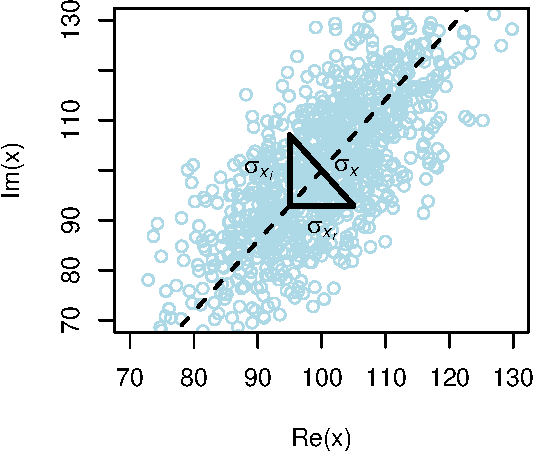
\includegraphics{Svetunkov---Svetunkov---Complex-Valued-Econometrics_files/figure-latex/crvMomentSecondVariance-1.pdf}
\caption{\label{fig:crvMomentSecondVariance}Visual representation of variance of a complex random variable.}
\end{figure}

Figure \ref{fig:crvMomentSecondVariance} demonstrates graphically the relation between standard deviations of real, imaginary and the overall variance of a complex variable according to the formula \eqref{eq:crvMomentSecondVarianceShort}.

\citet{Picinbono} note that the moment \eqref{eq:crvMomentSecondVarianceShort} is not sufficient to entirely describe the second order statistics of a c.r.v. This is because it ignores the potential covariance between the parts of a variable and only describes their average variability. Another measure of variability of a complex random variable is the so called ``pseudo-variance'' \citep{reference}, which can be obtained by applying the conventional formula of variance directly to the c.r.v. without the multiplication by conjugate:
\begin{equation}
    \begin{aligned}
    \mathcal{V}(\underline{x}) = \varsigma_x^2 = & \mathrm{E}((\underline{x}-\underline{\mu})^2) = \mathrm{E}\left(((x_r-\mu_{r}) + i (x_i-\mu_{i}))^2\right) = \\
                    & \mathrm{E}((x_r-\mu_{r})^2) - \mathrm{E}((x_i-\mu_{i})^2) + i2 \mathrm{E}((x_r-\mu_{r})(x_i-\mu_{i}))
    \end{aligned}
    \label{eq:crvMomentSecondVariancePseudo}
\end{equation}
or using the notation \(\sigma_{x_r,x_i}\) for covariance between the real and imaginary parts:
\begin{equation}
    \varsigma_x^2 = \sigma_{x_r}^2 - \sigma_{x_i}^2 + i2 \sigma_{x_r,x_i}.
    \label{eq:crvMomentSecondVariancePseudoShort}
\end{equation}
In the literature, the moment \eqref{eq:crvMomentSecondVariancePseudoShort} is called pseudo-variance \citep{reference}, because it does not measure the variability of a variable, but rather gives a different information: it shows whether the real and imaginary variances are similar and what the covariance between them is. If both real and imaginary parts of \eqref{eq:crvMomentSecondVariancePseudoShort} are equal to zero then it is said that the distribution of the complex variable \(x\) is spherical \citep{reference}, i.e.~the variances are similar and the real and imaginary parts are not linearly related. Furthermore, we should point out that while minimising \eqref{eq:crvMomentSecondVarianceShort} implies minimising both variances of the real and imaginary parts of \(x\) (ignoring the covariance between them), minimising \eqref{eq:crvMomentSecondVariancePseudoShort} is not as straightforward. At very least, we could tell that it implies making the distribution of \(x\) closer to the spherical one, but we cannot provide any thorough insight about this.

We should note that both measures can be considered as complex, and the main distinction between them is the multiplication by the same c.r.v or by its conjugate. As such we propose to call them respectively ``conjugate variance'' and ``direct variance''.

Having calculated the two variances, we can then extract variances of real and imaginary parts and the covariance between them via formulae (which follows directly from \eqref{eq:crvMomentSecondVarianceShort} and \eqref{eq:crvMomentSecondVariancePseudoShort}):
\begin{equation}
    \begin{aligned}
        & \sigma_{x_r}^2 = \frac{\mathcal{R}(\sigma^2_x) + \mathcal{R}(\varsigma^2_x)}{2} \\
        & \sigma_{x_i}^2 = \frac{\mathcal{R}(\sigma^2_x) - \mathcal{R}(\varsigma^2_x)}{2} \\
        & \sigma_{x_r,x_i} = \frac{\mathcal{I}(\varsigma^2_x)}{2}
    \end{aligned} .
    \label{eq:IndividualVariances}
\end{equation}
These individual real-valued moments might be useful in case of hypothesis testing or constructing confidence intervals for each of the parts of c.r.v. independently.

In R, the conjugate and direct variances are available in \texttt{cvar()} function of \texttt{complex} package.

\begin{Shaded}
\begin{Highlighting}[]
\CommentTok{\# Create a random variable}
\NormalTok{x \textless{}{-}}\StringTok{ }\KeywordTok{complex}\NormalTok{(}\DataTypeTok{real=}\KeywordTok{rnorm}\NormalTok{(}\DecValTok{100}\NormalTok{, }\DataTypeTok{mean=}\DecValTok{50}\NormalTok{, }\DataTypeTok{sd=}\DecValTok{5}\NormalTok{),}
             \DataTypeTok{imaginary=}\KeywordTok{rnorm}\NormalTok{(}\DecValTok{100}\NormalTok{, }\DataTypeTok{mean=}\DecValTok{100}\NormalTok{, }\DataTypeTok{sd=}\DecValTok{10}\NormalTok{))}
\CommentTok{\# Calculate the conjugate variance}
\KeywordTok{cvar}\NormalTok{(x, }\DataTypeTok{method=}\StringTok{"conjugate"}\NormalTok{) }\OperatorTok{|}\ErrorTok{\textgreater{}}
\StringTok{    }\KeywordTok{setNames}\NormalTok{(}\StringTok{"Conjugate variance"}\NormalTok{)}
\end{Highlighting}
\end{Shaded}

\begin{verbatim}
## Conjugate variance 
## 133.1791+0i
\end{verbatim}

\begin{Shaded}
\begin{Highlighting}[]
\CommentTok{\# Calculate the direct variance}
\KeywordTok{cvar}\NormalTok{(x, }\DataTypeTok{method=}\StringTok{"direct"}\NormalTok{) }\OperatorTok{|}\ErrorTok{\textgreater{}}
\StringTok{    }\KeywordTok{setNames}\NormalTok{(}\StringTok{"Direct variance"}\NormalTok{)}
\end{Highlighting}
\end{Shaded}

\begin{verbatim}
##    Direct variance 
## -86.09531+8.43144i
\end{verbatim}

As we see from the output above, the direct variance has the negative real part, which indicates that the imaginary part has higher variance than the real one. The imaginary part of the direct variance shows the double covariance between the real and imaginary parts. Finally, the conjugate variance should be \(5^2 + 10^2 = 125\), but due to small sample (100 observations in the generated random variable above), it will be equal to a number close to it.

Given that any complex variable can be represented in a vector form, the c.r.v. \(x\) can be treated as a bivariate random variable, for which a covariance matrix can be calculated via:
\begin{equation}
    \boldsymbol{\Sigma}_x = \begin{pmatrix} \sigma_{x_r}^2 & \sigma_{x_r, x_i} \\ \sigma_{x_r, x_i} & \sigma_{x_i}^2 \end{pmatrix} .
    \label{eq:crvMomentSecondVarianceMatrix}
\end{equation}
The minimisation of the matrix \eqref{eq:crvMomentSecondVarianceMatrix} does not make sense, but instead it is possible to minimise the determinant of that matrix, which is called ``Generalised Variance'' (GV):
\begin{equation}
    \mathrm{GV} = |\boldsymbol{\Sigma}_x| = \sigma_{x_r}^2 \sigma_{x_i}^2 - \sigma_{x_r, x_i}^2 .
    \label{eq:crvMomentSecondGV}
\end{equation}

In R, this is implemented in \texttt{covar()} function from the \texttt{complex} package:

\begin{Shaded}
\begin{Highlighting}[]
\KeywordTok{covar}\NormalTok{(x)}
\end{Highlighting}
\end{Shaded}

\begin{verbatim}
##           x_r        x_i
## x_r 23.541914   4.215722
## x_i  4.215722 109.637224
\end{verbatim}

The minimisation of GV, as can be seen from the formula \eqref{eq:crvMomentSecondGV}, implies the simultaneous minimisation of variances of real and imaginary parts and maximisation of the square of covariance between them, making the resulting distribution compacter and emphasising the potential relations between the real and imaginary parts of a c.r.v. For our example in R, the GV equals to:

\begin{Shaded}
\begin{Highlighting}[]
\KeywordTok{covar}\NormalTok{(x) }\OperatorTok{|}\ErrorTok{\textgreater{}}\StringTok{ }\KeywordTok{det}\NormalTok{()}
\end{Highlighting}
\end{Shaded}

\begin{verbatim}
## [1] 2563.298
\end{verbatim}

All the three moments discussed in this subsection rely on variances of real and imaginary parts of a c.r.v. and on a covariance between those parts. These moments in turn can be calculated using the conventional formulae, correcting for the potential small sample bias \citep{referenceSBA}:
\begin{equation}
    \begin{aligned}
        \hat{\sigma}_{x_r}^2 = & \frac{1}{n-k} \sum_{j=1}^n (x_{r,j}-\bar{x}_{r,j})^2 \\
        \hat{\sigma}_{x_i}^2 = & \frac{1}{n-k} \sum_{j=1}^n (x_{i,j}-\bar{x}_{i,j})^2 \\
        \hat{\sigma}_{x_r, x_i} = & \frac{1}{n-k} \sum_{j=1}^n (x_{r,j}-\bar{x}_{r,j})(x_{i,j}-\bar{x}_{i,j})^2 ,
    \end{aligned}
    \label{eq:crvMomentSecondSample}
\end{equation}
where \(k\) is the number of estimated parameters in a model.

Finally, similar to the variance it is possible to calculate second moments between two complex random variables \(x = x_r+i x_i\) and \(y = y_r + i y_i\) \citep{Picinbono}. The ``conjugate'' covariance is calculated similarly to \eqref{eq:crvMomentSecondVariance} via the multiplication by conjugate:
\begin{equation}
    \begin{aligned}
    \sigma_{x,y} = & \mathrm{E}((\tilde{x}-\tilde{\mu}_x) (y-\mu_y)) = \\
                   & \mathrm{E}\left(((x_r-\mu_{x,r}) - i (x_i-\mu_{x,i}))((y_r-\mu_{y,r}) + i (y_i-\mu_{y,i}))\right) = \\
                   & \mathrm{E}((x_r-\mu_{x,r})(y_r-\mu_{y,r})) + \mathrm{E}((x_i-\mu_{x,i})(y_i-\mu_{y,i})) + \\
                   & i \left(\mathrm{E}((x_r-\mu_{x,r})(y_i-\mu_{y,i})) - \mathrm{E}((x_i-\mu_{x,i})(y_r-\mu_{y,r}))\right)
    \end{aligned}
    \label{eq:crvMomentSecondCovariance}
\end{equation}
where \(\mu_{x}\) and \(\mu_y\) are the respective first moments of c.r.v. \(x\) and \(y\). Using the notations above, the same covariance can be rewritten as:
\begin{equation}
    \sigma_{x,y} = \sigma_{x_r, y_r} + \sigma_{x_i, y_i} + i (\sigma_{x_r, y_i} - \sigma_{x_i, y_r}),
    \label{eq:crvMomentSecondCovarianceShort}
\end{equation}
which similarly to the variance \eqref{eq:crvMomentSecondVarianceShort} mixes the moments of the real and imaginary parts of the two random variables. Note though that if the conjugate of \(y\) is used instead of the conjugate of \(x\), the imaginary part of the covariance \eqref{eq:crvMomentSecondCovarianceShort} will change to \(\sigma_{x_i, y_r} - \sigma_{x_r, y_i}\), giving potentially different information about the relation between the variables.

In order to have more information about a c.r.v., we also need to consider the ``direct'' covariance \citep[also known in the literature as pseudo-covariance,][]{reference}, which can be shown to be equal to:
\begin{equation}
    \varsigma_{x,y} = \sigma_{x_r, y_r} - \sigma_{x_i, y_i} + i (\sigma_{x_i, y_r} + \sigma_{x_r, y_i}).
    \label{eq:crvMomentSecondPseudoCovarianceShort}
\end{equation}
Note that none of these moments on its own gives enough information about the relation between two complex variables, so they need to be used jointly. Alternatively, using vector representation, a covariance matrix between the two c.r.v. can be used to get a better understanding about the relations between them:
\begin{equation}
    \boldsymbol{\Sigma}_{x,y} =
        \begin{pmatrix}
            \sigma_{x_r}^2 & \sigma_{x_r, x_i} & \sigma_{x_r, y_r} & \sigma_{x_r, y_i} \\
            \sigma_{x_r, x_i} & \sigma_{x_i}^2 & \sigma_{x_i, y_r} & \sigma_{x_i, y_i} \\
            \sigma_{x_r, y_r} & \sigma_{x_i, y_r} & \sigma_{y_r}^2 & \sigma_{y_r, y_i} \\
            \sigma_{x_r, y_i} & \sigma_{x_i, y_i} & \sigma_{y_r, y_i} & \sigma_{y_i}^2
        \end{pmatrix} .
    \label{eq:crvMomentSecondCoVarianceMatrix}
\end{equation}

In R, the complex covariances are implemented in \texttt{ccov()} function from the \texttt{complex} package:

\begin{Shaded}
\begin{Highlighting}[]
\CommentTok{\# Create a random variable x}
\NormalTok{x \textless{}{-}}\StringTok{ }\KeywordTok{complex}\NormalTok{(}\DataTypeTok{real=}\KeywordTok{rnorm}\NormalTok{(}\DecValTok{100}\NormalTok{, }\DataTypeTok{mean=}\DecValTok{50}\NormalTok{, }\DataTypeTok{sd=}\DecValTok{5}\NormalTok{),}
             \DataTypeTok{imaginary=}\KeywordTok{rnorm}\NormalTok{(}\DecValTok{100}\NormalTok{, }\DataTypeTok{mean=}\DecValTok{100}\NormalTok{, }\DataTypeTok{sd=}\DecValTok{10}\NormalTok{))}
\CommentTok{\# Create a random variable y}
\NormalTok{y \textless{}{-}}\StringTok{ }\NormalTok{(}\FloatTok{1.5} \OperatorTok{+}\StringTok{ }\NormalTok{3i) }\OperatorTok{+}\StringTok{ }\NormalTok{(}\FloatTok{0.5} \OperatorTok{{-}}\StringTok{ }\FloatTok{0.75}\NormalTok{i) }\OperatorTok{*}\StringTok{ }\NormalTok{x }\OperatorTok{+}
\StringTok{            }\KeywordTok{complex}\NormalTok{(}\DataTypeTok{real=}\KeywordTok{rnorm}\NormalTok{(}\DecValTok{100}\NormalTok{, }\DataTypeTok{mean=}\DecValTok{0}\NormalTok{, }\DataTypeTok{sd=}\DecValTok{10}\NormalTok{),}
                    \DataTypeTok{imaginary=}\KeywordTok{rnorm}\NormalTok{(}\DecValTok{100}\NormalTok{, }\DataTypeTok{mean=}\DecValTok{0}\NormalTok{, }\DataTypeTok{sd=}\DecValTok{10}\NormalTok{))}
\CommentTok{\# Calculate the conjugate variance}
\KeywordTok{ccov}\NormalTok{(x, y, }\DataTypeTok{method=}\StringTok{"conjugate"}\NormalTok{) }\OperatorTok{|}\ErrorTok{\textgreater{}}
\StringTok{    }\KeywordTok{setNames}\NormalTok{(}\StringTok{"Conjugate covariance"}\NormalTok{)}
\end{Highlighting}
\end{Shaded}

\begin{verbatim}
## Conjugate covariance 
## 41.1105-107.0509i
\end{verbatim}

\begin{Shaded}
\begin{Highlighting}[]
\CommentTok{\# Calculate the direct variance}
\KeywordTok{ccov}\NormalTok{(x, y, }\DataTypeTok{method=}\StringTok{"direct"}\NormalTok{) }\OperatorTok{|}\ErrorTok{\textgreater{}}
\StringTok{    }\KeywordTok{setNames}\NormalTok{(}\StringTok{"Direct covariance"}\NormalTok{)}
\end{Highlighting}
\end{Shaded}

\begin{verbatim}
##   Direct covariance 
## -22.86722+64.19287i
\end{verbatim}

The functions \texttt{cvar()} and \texttt{ccov()} also accept a matrix instead of vector \texttt{x}, in which case they will produce a matrix of moments with complex variances on diagonal and complex covariances on the off-diagonals.

\begin{Shaded}
\begin{Highlighting}[]
\NormalTok{ourData \textless{}{-}}\StringTok{ }\KeywordTok{cbind}\NormalTok{(x,y)}
\KeywordTok{cvar}\NormalTok{(ourData, }\DataTypeTok{method=}\StringTok{"direct"}\NormalTok{)}
\end{Highlighting}
\end{Shaded}

\begin{verbatim}
##                     x                   y
## x -84.47425+ 1.62613i -22.86722+64.19287i
## y -22.86722+64.19287i  54.28555- 5.38777i
\end{verbatim}

While there exist higher order moments for complex random variables, we do not discuss them in this book.

\hypertarget{parametric-distributions-of-c.r.v.}{%
\section{Parametric Distributions of c.r.v.}\label{parametric-distributions-of-c.r.v.}}

Similarly to the real valued random variables, complex random variables can follow some parametric distributions. In this section, we discuss several simple ones, some of which will be used later in this monograph.

In general, it is reasonable to assume that a c.r.v. has a distribution of a shape of a circle or ellipse on the complex plane. This becomes more apparent if we consider the exponential form of a c.r.v. \eqref{eq:complexNumberExponential} and consider both magnitude and the angle as random variables. In the simplest case, when they are not correlated and we consider a variable that is centred around the origin, the randomness coming from both of these components will result in a circle on the complex plane, see the following example in R (and Figure \ref{fig:crvGeneratedCircle}):

\begin{Shaded}
\begin{Highlighting}[]
\CommentTok{\# Generate magnitudes from the uniform distribution}
\NormalTok{R \textless{}{-}}\StringTok{ }\KeywordTok{runif}\NormalTok{(}\DecValTok{1000}\NormalTok{,}\DecValTok{0}\NormalTok{,}\DecValTok{10}\NormalTok{)}
\CommentTok{\# Generate angles from the uniform distribution}
\NormalTok{phi \textless{}{-}}\StringTok{ }\KeywordTok{runif}\NormalTok{(}\DecValTok{1000}\NormalTok{,}\OperatorTok{{-}}\NormalTok{pi,pi)}
\CommentTok{\# Create c.r.v in exponential form}
\NormalTok{x \textless{}{-}}\StringTok{ }\NormalTok{R }\OperatorTok{*}\StringTok{ }\KeywordTok{exp}\NormalTok{(}\KeywordTok{complex}\NormalTok{(}\DataTypeTok{imaginary=}\NormalTok{phi))}
\CommentTok{\# Plot the variable}
\KeywordTok{plot}\NormalTok{(x)}
\end{Highlighting}
\end{Shaded}

\begin{figure}
\centering
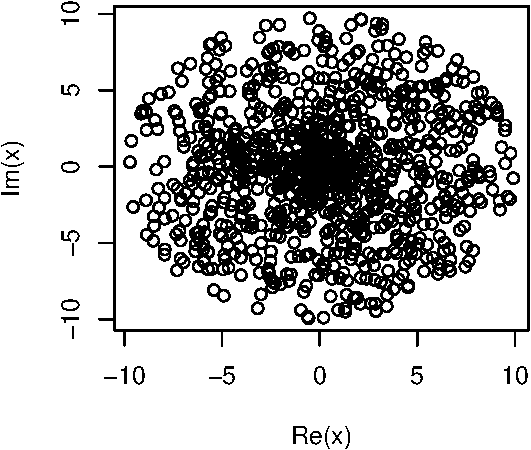
\includegraphics{Svetunkov---Svetunkov---Complex-Valued-Econometrics_files/figure-latex/crvGeneratedCircle-1.pdf}
\caption{\label{fig:crvGeneratedCircle}C.r.v. generated from a uniform distribuiton.}
\end{figure}

The example in Figure \ref{fig:crvGeneratedCircle} demonstrates how a c.r.v. with uncorrelated real and imaginary parts looks on the complex plane. If there is a relation between the parts then the circle transforms into ellipse. So, it is only logical to consider the distributions that rely on a circle or an ellipse for the c.r.v. instead of any other geometric shapes.

When it comes to distribution functions, in case of c.r.v. in general we should consider the joint bivariate distribution, thus all the probability density and cumulative distribution functions will be plotted in 3D with the density/probability in z-axis and the complex variable in x and y axes.

\hypertarget{distributionCNorm}{%
\subsection{Complex Normal distribution}\label{distributionCNorm}}

One of the most popular distributions in statistics is the Normal distribution. There exists a complex counterpart of that distribution, which has the following probability density function \citep{refGoodman}:
\begin{equation}
    f(\underline{x}) = \frac{1}{\pi^2 \sqrt{\sigma^4 - \varsigma^2 \tilde{\varsigma}^2}} \exp\left(- \frac{1}{2}
        \begin{pmatrix} \underline{\tilde{x}} - \underline{\tilde{\mu}} & \underline{x} - \underline{\mu} \end{pmatrix}
        \begin{pmatrix} \sigma^2 & \varsigma^2 \\ \tilde{\varsigma}^2 & \sigma^2 \end{pmatrix}^{-1}
        \begin{pmatrix} \underline{x} - \underline{\mu} \\ \underline{\tilde{x}} - \underline{\tilde{\mu}} \end{pmatrix}
    \right),
    \label{eq:ComplexNormalPDF}
\end{equation}
where \(\underline{\mu}\) is the first moment of the c.r.v. \(\underline{x}\) and \(\sigma^2\) and \(\varsigma^2\) are the conjugate and direct variances as defined in Section \ref{complexRandomVariable}. The variable that follows this distribution can be denoted as \(\underline{x} \sim \mathcal{CN}(\underline{\mu}, \sigma^2, \varsigma^2)\) Note that both \(\sigma^2\) and \(\varsigma^2\) are important in the PDF \eqref{eq:ComplexNormalPDF} to define the shape of the distribution. For the real-valued variables, the conventional standard deviation \(\sigma\) characterises the dispersion of the random variable, and in case of the normal distribution shows how many z-scores away the random variable can lie from its centre. For the c.r.v., \(\sigma\) plays a similar role, but not in terms of units along the x axis, but rather in terms of radii from the centre. The direct variance \(\varsigma^2\), on the other hand characterises the shape of the distribution itself: its real part shows whether the ellipse of the normal distribution should be wide (positive numbers) or narrow (negative numbers), while the imaginary part shows how close the points should be to the line drawn through them. These moments are shown visually in Figure \ref{fig:crvNormalMoments}.

\begin{figure}
\centering
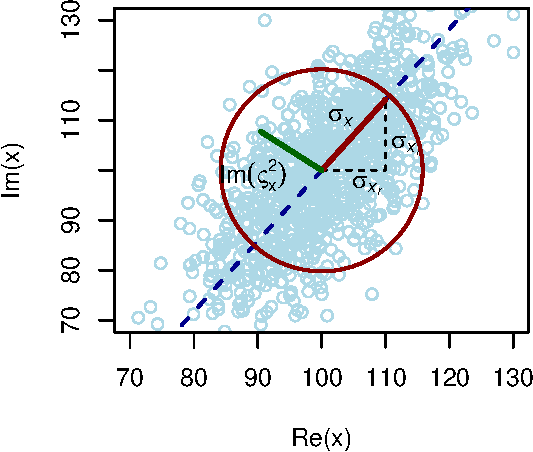
\includegraphics{Svetunkov---Svetunkov---Complex-Valued-Econometrics_files/figure-latex/crvNormalMoments-1.pdf}
\caption{\label{fig:crvNormalMoments}Visual representation of variances for a c.r.v. that follows Complex Normal distribution.}
\end{figure}

The overall conjugate standard deviation \(\sigma_x\) represents the radius of the unit circle in Figure \ref{fig:crvNormalMoments}, while the imaginary part of \(\varsigma_x^2\) (i.e.~\(2 \sigma_{x_r, x_i}\)) is shown with a green line. The real part of \(\varsigma_x^2\) is not visualised, but for this plot it will be negative, showing that the distribution is narrower along the x-axis than along the y-axis.

Figure \ref{fig:plotlyCNormal} shows the PDF of \(x \sim \mathcal{CN}(100+100i,100,-20+i30)\), while Figure \ref{fig:plotlyCNormalHeatmap} shows the heatmap of the same PDF. The brighter areas in both Figures correspond to the higher values of PDF. For each specific value of density, there is a multitude of values of \(x\), forming an ellipse of a specific length.

\begin{figure}
\centering
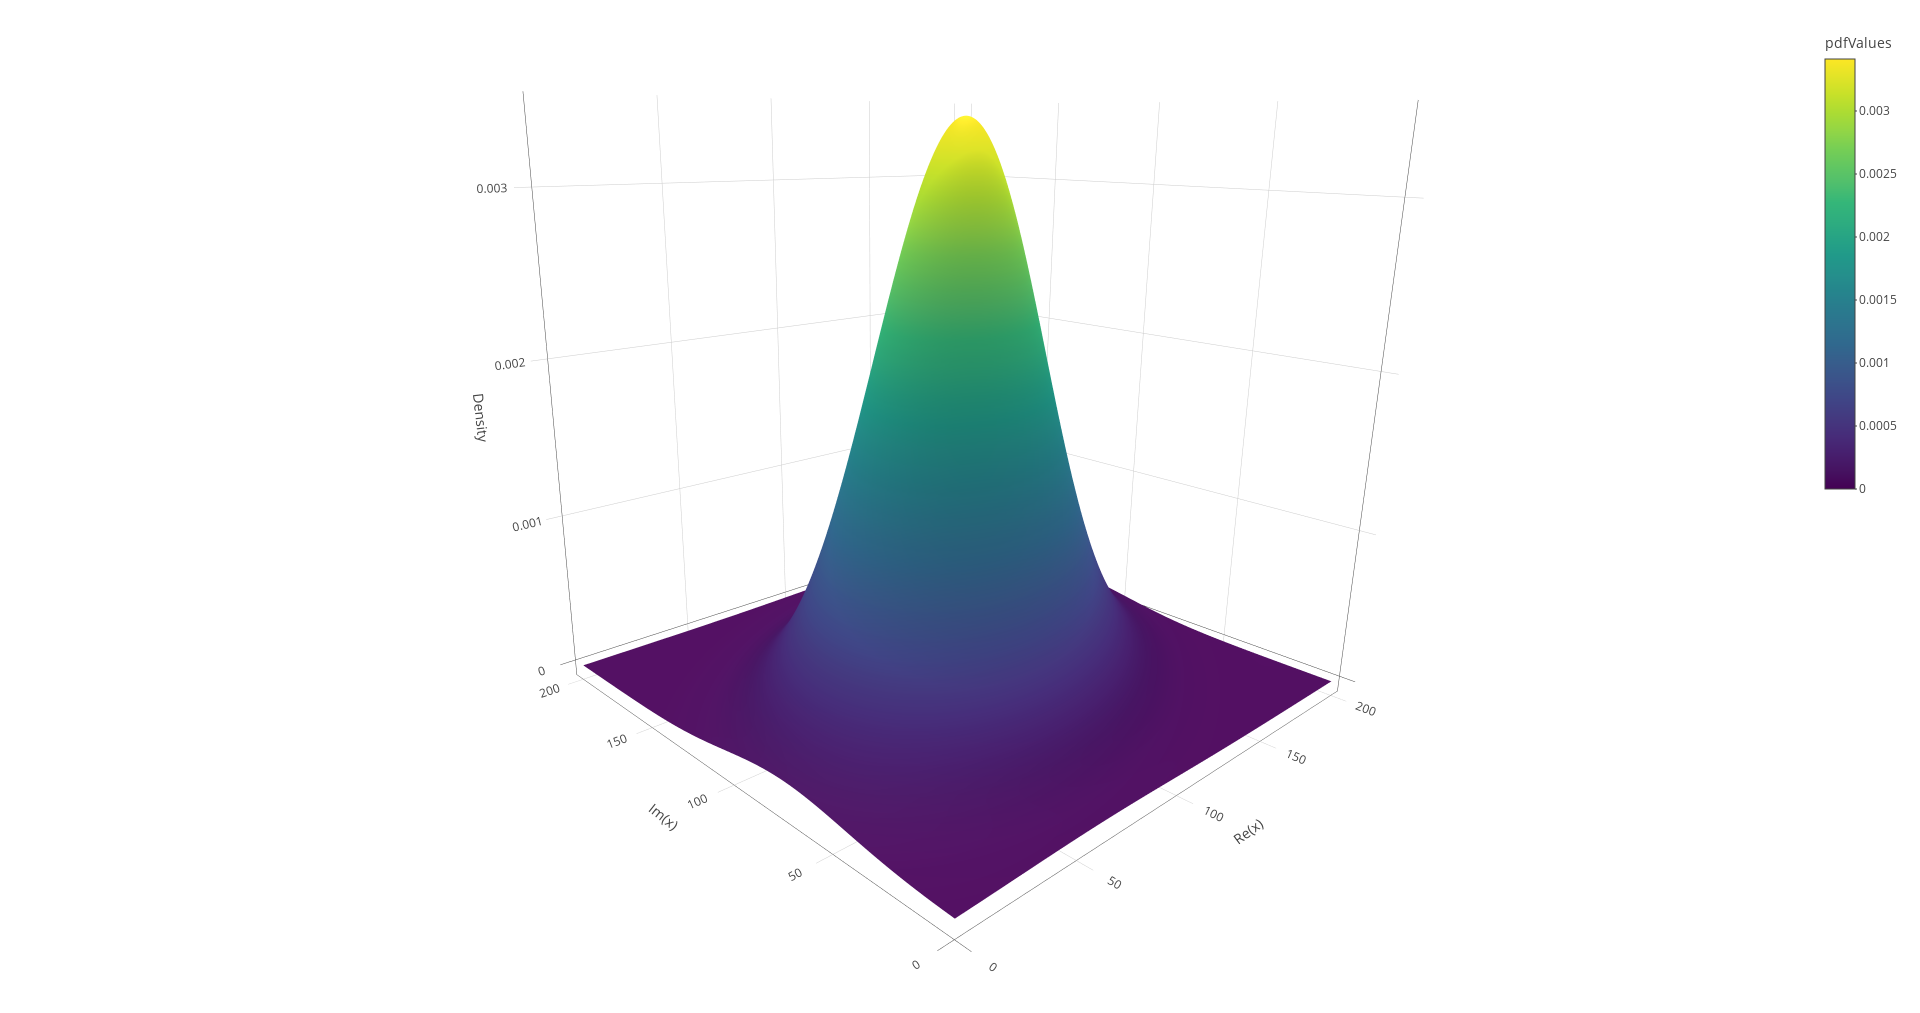
\includegraphics{./images/plotlyCNormal.png}
\caption{\label{fig:plotlyCNormal}Plot of the probability density function of complex normal distribution.}
\end{figure}

\begin{figure}
\centering
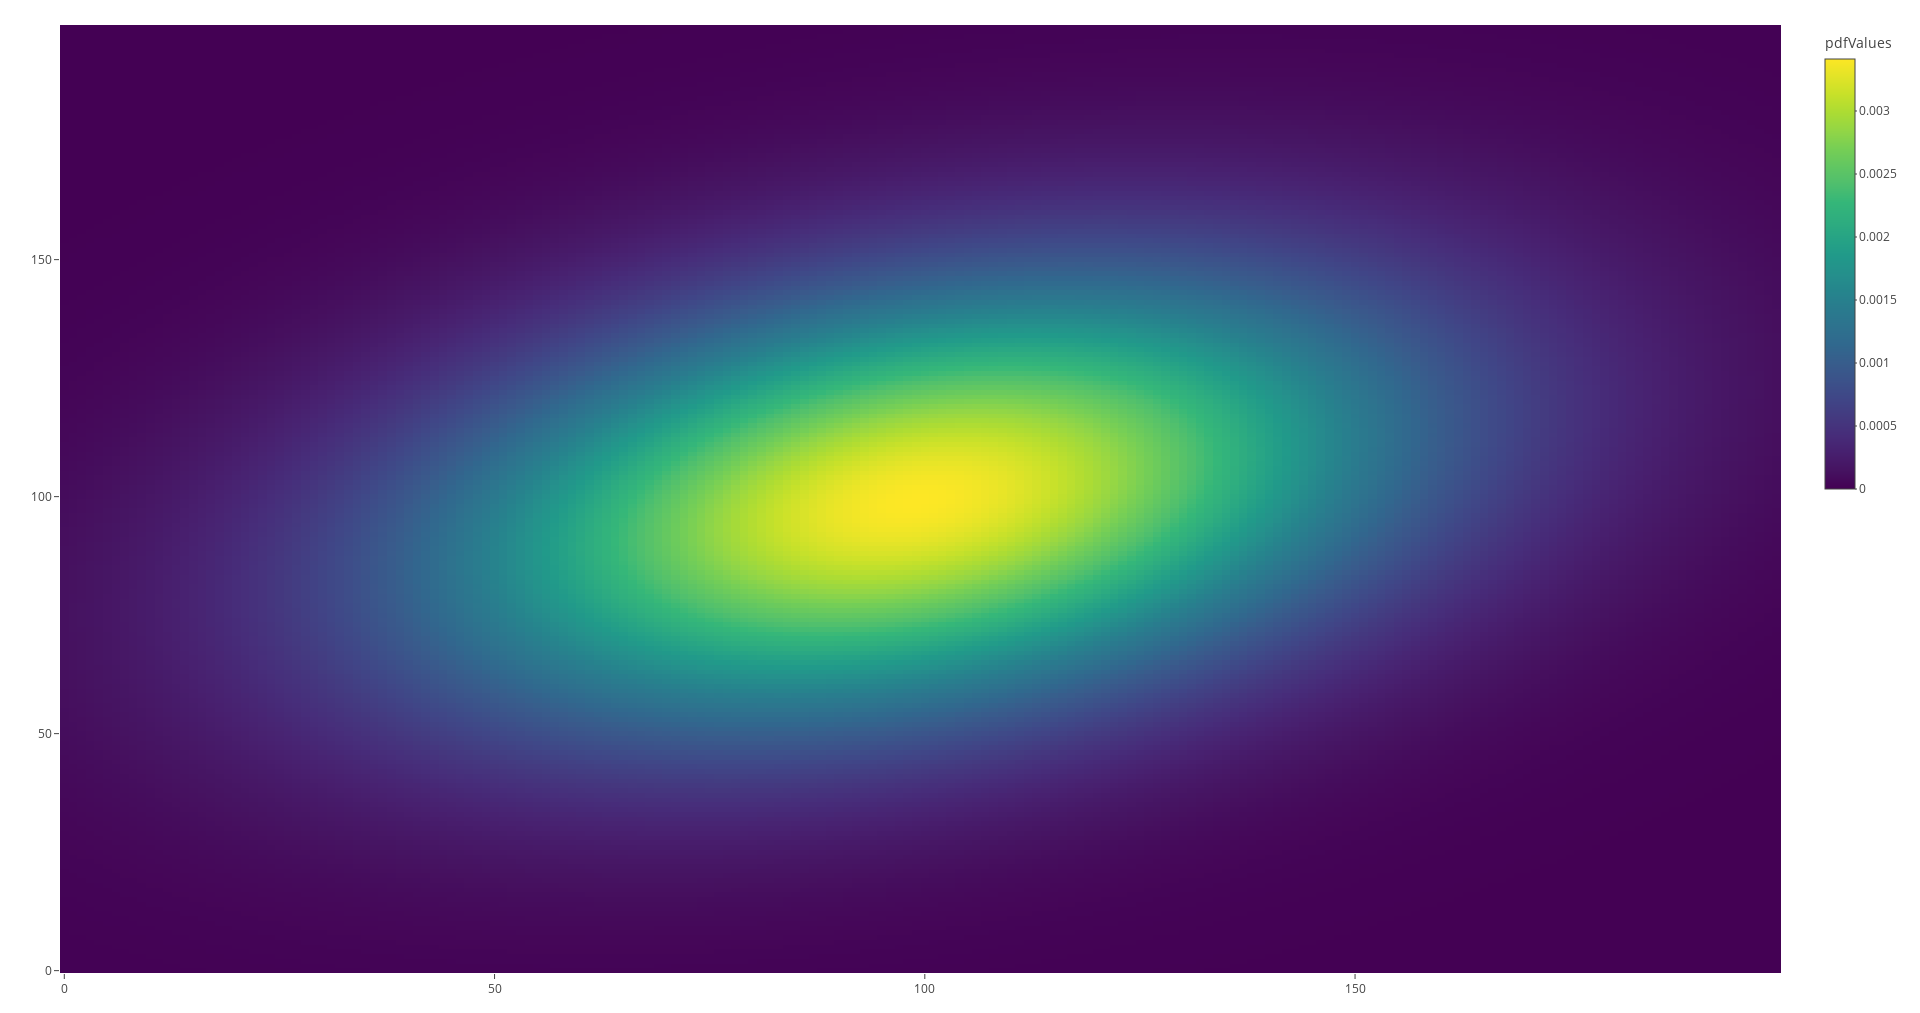
\includegraphics{./images/plotlyCNormalHeatmap.png}
\caption{\label{fig:plotlyCNormalHeatmap}Heatmap of density of Complex Normal distribution.}
\end{figure}

One special case of a Complex Normal distribution is a so called ``Circular Symmetric'' Complex Normal distribution. It is a distribution for which the direct variance equals to zero, which implies that the variances of the real and the imaginary parts are equal and that the covariance between them is equal to zero. This specific distribution is used extensively in signal processing literature \citep{referenceHere}.

The functions of the Complex Normal distribution are implemented as \texttt{dcnorm()}, \texttt{pcnorm()}, \texttt{qmcnorm()} and \texttt{rmcnorm()} in the \texttt{complex} package.

The Complex Normal distribution can be used for the joint estimation of parameters of a complex-valued model and for generation of prediction intervals from it. However, in some cases it might be more convenient to consider a c.r.v. model as a bivariate vector model based on \eqref{eq:complexFunctionVectors} and thus to revert to the multivariate normal distribution.

\hypertarget{MVNorm}{%
\subsection{Multivariate Normal distribution}\label{MVNorm}}

The same normal distribution for a complex variable can be parametrised via a covariance matrix \(\boldsymbol{\Sigma}\) from \eqref{eq:crvMomentSecondVarianceMatrix} instead of the conjugate and direct variances \(\sigma^2\) and \(\varsigma^2\). In general, the Probability Density Function for a vector of \(n\) variables can be written as:
\begin{equation}
    f(\mathbf{x}) = \frac{1}{(2 \pi)^{\frac{n}{2}} \sqrt{|\boldsymbol{\Sigma}|}} \exp\left(- \frac{1}{2}
        \begin{pmatrix} \mathbf{x} - \boldsymbol{\mu} \end{pmatrix}^\top \boldsymbol{\Sigma}^{-1} \begin{pmatrix} \mathbf{x} - \boldsymbol{\mu} \end{pmatrix}
    \right).
    \label{eq:MultivariateNormalPDF}
\end{equation}
For the bivariate case of a c.r.v. represented in a form of a vector, \(n=2\) and the covariance matrix \(\boldsymbol{\Sigma}\) has dimensionality of \(2 \times 2\). In that case the PDF will be the same as for the Complex Normal distribution. In fact, it is possible to recreate the covariance matrix based on the values of conjugate and direct variances:
\begin{equation}
    \boldsymbol{\Sigma} = \frac{1}{2} \begin{pmatrix} \mathcal{R}(\sigma^2) + \mathcal{R}(\varsigma^2) & \mathcal{I}(\varsigma^2) \\
                                                      \mathcal{I}(\varsigma^2) & \mathcal{R}(\sigma^2) - \mathcal{R}(\varsigma^2) \end{pmatrix} .
    \label{eq:MultivariateNormalPDFCovariance}
\end{equation}

When it comes to constructing confidence regions from the multivariate normal distribution then the following inequality is used to determine values of the vector of quantiles \(\mathbf{q}\):
\begin{equation}
    (\mathbf{x} - \mathbf{q})^{\top} \mathbf{\Sigma}^{-1} (\mathbf{x} - \mathbf{q}) \leq \chi^2(n, p) ,
    \label{eq:MultivariateNormalRegion}
\end{equation}
where \(p\) is the confidence level. For the case of c.r.v., when \(n=2\), the \(\chi^2(n, p)\) transforms into the exponential distribution \(\mathcal{E}(0.5)\).

Note however that working with confidence regions is challenging, because there is an infinite number of values of the vector \(\mathbf{q}\) that give the same critical value \(\chi^2(n, p)\). So, in order to make it practical, unconditional prediction intervals can be constructed for each of the parts, dropping the other one. In this case, the classical formula for the intervals can be used, for example for the real part of the c.r.v.:
\begin{equation}
    x_{r} \in \left( \mu_{x_r} + \sigma_{x_r} z \left({\frac{\alpha}{2}} \right) , \mu_{x_r} + \sigma_{x_r} z \left({\frac{1+\alpha}{2}} \right) \right),
    \label{eq:NormalInterval}
\end{equation}
where \(z\left({\frac{\alpha}{2}} \right)\) and \(z\left({\frac{1+\alpha}{2}} \right)\) are the respective lower and upper quantiles of the standard normal distribution.

\hypertarget{Hotelling}{%
\subsection{Hotelling's T-squared distribution}\label{Hotelling}}

When it comes to distribution of complex variables statistics, one of the most important ones is a distribution of a mean of a complex variable. In the case of real variables, it is well known that if the Central Limit Theorem (CLT) holds then the sample mean will follow Normal distribution, and confidence interval for the mean can be constructed using Student's t distribution (when the population variance is unknown, i.e.~in reality). For c.r.v., the situation is similar: when CLT holds, the c.r.v. follows Complex Normal distribution, but instead of Student's t distribution, we need to use its multivariate counterpart, which is called ``Hotelling's T-squared'' distribution. It is more convenient to consider the statistics for a c.r.v in a vector form (i.e.~treat it as bivariate). If we estimate the sample mean \(\hat{\boldsymbol{\mu}}_x\) and a sample covariance matrix of the mean \(\hat{\boldsymbol{\Sigma}}_{\mu_{x}}\) then the following holds (if CLT holds):
\begin{equation}
    (\hat{\boldsymbol{\mu}}_x - \boldsymbol{\mu}_x)^\prime \hat{\boldsymbol{\Sigma}}_{\mu_{x}}^{-1} (\hat{\boldsymbol{\mu}}_x - \boldsymbol{\mu}_x) \sim T^2(2, n-1) = \frac{2(n-1)}{n-2} F(2, n-2),
    \label{eq:hotellingT}
\end{equation}
where \(T^2(2, n-1)\) is a T-squared Hotelling's statistics with 2 and \(n-1\) degrees of freedom, and \(F(2, n-2)\) is the Fisher's distribution statistics with 2 and \(n-2\) degrees of freedom. Equation \eqref{eq:hotellingT} can be used to construct confidence interval for a multivariate mean or for testing statistical hypotheses. One of the possible hypotheses that would make sense in case of c.r.v. and could be tested based on \eqref{eq:hotellingT} is the following:
\begin{equation}
    \begin{aligned}
        & \mathrm{H}_0: \boldsymbol{\mu}_x = 0 \\
        & \mathrm{H}_1: \boldsymbol{\mu}_x \neq 0
    \end{aligned}
    \label{eq:hypothesisFirst}
\end{equation}
or equivalently:
\begin{equation}
    \begin{aligned}
        & \mathrm{H}_0: \mu_{x_r} = \mu_{x_i} = 0 \\
        & \mathrm{H}_1: \mu_{x_r} \neq 0 \vee \mu_{x_i} \neq 0
    \end{aligned}
    \label{eq:hypothesisSecond}
\end{equation}
However, from practical point of view, testing the joint hypothesis \eqref{eq:hypothesisSecond} might not be very useful. Instead, testing the classical hypotheses from the univariate context based on Student's t distribution for each part of c.r.v. might provide more detailed information, i.e.~whether the specific real or imaginary part of the variable equals to zero or not. In contrast, in case of the hypothesis \eqref{eq:hypothesisSecond}, rejecting the null hypothesis implies that something is not equal to zero, but it is not clear, what specifically.

\hypertarget{complexModelling}{%
\section{Complex-valued Modelling}\label{complexModelling}}

Now that we have discussed basics of complex variables theory, we can discuss the modelling aspects: it might not look straightforward, what should be included in the real and the imaginary part of a complex variable. There are two philosophical views on complex-valued modelling:

\begin{enumerate}
\def\labelenumi{\arabic{enumi}.}
\tightlist
\item
  You need to find processes, where complex variables arise naturally;
\item
  You can model anything with complex variables as long as you follow some rules.
\end{enumerate}

If you follow the former view you need to find some variables that form two parts of the whole that work together. An example of this case is the wind power and direction forecasting. The two variables in this case will be naturally represented in the exponential form:
\begin{equation*}
    \underline{y} = r \mathrm{e}^{i \phi} ,
\end{equation*}
where \(r\) is the power of wind and \(\phi\) is its direction. In this formulation, we can then model, for example, how the two characteristics of wind on some observation \(t\) depend on the previous values and some external information:
\begin{equation*}
    \underline{y}_t = f(\underline{y}_{t-1}, \underline{y}_{t-2}, \dots, \underline{y}_{t-p}, \underline{\mathbf{x}}_t, \underline{\epsilon}_t),
\end{equation*}
where \(t\) is the index of the observation, \(p\) is the order of the model, \(\underline{\mathbf{x}}_t\) is the vector of all explanatory complex variables under consideration and \(\underline{\epsilon}_t\) is the error term. Some aspects of such a model are discussed in the Chapter \ref{multipleCLR} of this book, while the others are covered in Chapter \ref{Dynamic}.

However, it might be hard to find examples like the one with the wind above in economics and business domains. Trying to find something analogous (power + i direction) might lead us into a dead end. This is why the second philosophical view exists. \citet{Svetunkov2012} argues that any two variables can be united in a complex variable (in the arithmetic form) as long as:

\begin{enumerate}
\def\labelenumi{\arabic{enumi}.}
\tightlist
\item
  They reflect two sides of a process/phenomenon;
\item
  They have the same scale.
\end{enumerate}

The second condition implies that some sort of scaling is required if the variables have different scales. If this condition is not satisfied then the operations with complex variables might lead to meaningless results. For example, if we consider a variable of sales quantity and product price, \(q + ip\) and multiply it by a complex parameter \(a_r + i a_i\), we get a complex variable that has a strange combination in it:
\begin{equation}
    \underline{z} = (q + ip) (a_r + i a_i) = q a_r - p a_i + i(q a_i + p a_r).
    \label{eq:noScalingExample}
\end{equation}
In the equation \eqref{eq:noScalingExample}, the resulting real part includes the multiplication of the number of units sold times the parameter \(a_r\), while the imaginary part has the price (e.g.~in U.S. dollars) times the same parameter \(a_r\). If the both parts of the variable were scaled the parameter \(a_r\) would act as a transformer from one value to another. But if the both parts are not scaled then in one case it acts as a scaler of units, while the in the other one as a scaler of U.S. dollars, which does not make much sense. This example shows why the condition (2) above is important in complex-valued modelling.

The scaling itself can be done using one of the conventional ways:

\begin{enumerate}
\def\labelenumi{\alph{enumi}.}
\tightlist
\item
  Normalisation: subtract the minimum value from all the values and then divide by the range. This way the normalised variable will lie between 0 and 1;
\item
  Standardisation: subtract the mean and divide the variable by its standard deviation. This way we centre the variable and get rid of scale;
\item
  Any other form of scaling, where the division is done by the value of the variable, thus making it unitless.
\end{enumerate}

If we deal with time series data, an additional operation might be important - taking differences to make the data stationary (this is discussed in Section \ref{DynamicARIMA}). If we do not do that, the new values of the variable might lie outside of the range defined by the scaling.

Incidentally, the example with the wind power above abides to these two conditions, because the variable itself is represented in the exponential form, thus the condition will be satisfied automatically when we use formula \eqref{eq:complexNumberTrigonometric} to move to the arithmetic one. This variable does not require any additional transformations and can be treated as is.

Furthermore, based on the discussion in Subsection \ref{vectorComplexVariables}, we can note that the complex-valued models share some structural similarities with vector models, such as Vector Autoregression, when they are applied to two variables. From this angle, the complex-valued models can be considered as special cases of the vector ones, when some restrictions are imposed on the matrix of parameters. This important property gives the complex-valued models their power: they need fewer parameters to estimate in comparison with their vector counterparts.

\hypertarget{simpleCLR}{%
\chapter{Simple Complex Linear Regression}\label{simpleCLR}}

We start with the simplest Complex Linear Regression (cLR), which we call ``simple'', because it captures the relation between two variables. The main difference from the conventional Simple Linear Regression is that each of the variables is complex. This makes the model more complicated than the one in real numbers domain.

\hypertarget{simpleCLRModel}{%
\section{Model formulation}\label{simpleCLRModel}}

The simple Complex Linear Regression can be written as:
\begin{equation}
    \underline{y}_j = \underline{\beta}_0 + \underline{\beta}_1 \underline{x}_j + \underline{\epsilon}_j,
    \label{eq:SimpleCLRComplex}
\end{equation}
where \(j\) is the index for an observation and every parameter and variable is a complex number, i.e.~\(\underline{y}_j = y_{r,j}+i y_{i,j}\) is the complex response variable, \(\underline{x}_j = x_{r,j}+i x_{i,j}\) is the complex explanatory variable, \(\underline{\beta}_{l} = \beta_{l,r} + i \beta_{l,i}\) is the \(l\)-th parameter and \(\underline{\epsilon}_j = \epsilon_{r,j} + i \epsilon_{i,j}\) is the error term. For now, we do not make any specific assumptions about the distribution of the complex error term, we will come back to this later in this chapter. Inserting these values in \eqref{eq:SimpleCLRComplex} leads to:
\begin{equation}
    y_{r,j}+i y_{i,j} = (\beta_{0,r} + i \beta_{0,i}) + (\beta_{1,r} + i \beta_{1,i}) (x_{r,j}+i x_{i,j}) + (\epsilon_{r,j} + i \epsilon_{i,j}),
    \label{eq:SimpleCLR}
\end{equation}
which is in fact a multivariate model, capturing how the change of values in pair of variables \(x_r\), \(x_i\) leads to the change in the pair of variables \(y_r\) and \(y_i\). Given that any complex equation can be represented as a system of two equations, the model \eqref{eq:SimpleCLR} can be represented as a system of two linear regressions:
\begin{equation}
    \begin{aligned}
        y_{r,j} = & \beta_{0,r} + \beta_{1,r} x_{r,j} - \beta_{1,i} x_{i,j} + \epsilon_{r,j} \\
        y_{i,j} = & \beta_{0,i} + \beta_{1,r} x_{i,j} + \beta_{1,i} x_{r,j} + \epsilon_{i,j}
    \end{aligned}
    \label{eq:SimpleCLRSystem}
\end{equation}
This model captures a very specific dynamics between the real and imaginary parts, given that they share the same set of parameters for the slope. But most importantly it shows how each complex variable \(y\) relates to variable \(x\) in a four dimensional space. Note that the real and imaginary parts of \(y\) can be exchanged without a serious impact on the model: in that case the values of parameters would change, but the relation between \(x\) and \(y\) would stay the same. Similarly, changing \(x_r\) with \(x_i\) would only lead to different estimates of parameters, the general relation will hold.

Given that we deal with a sample of values, the model \eqref{eq:SimpleCLRComplex} can be represented in a vector form for all observations \(j\) from 1 to \(n\) (based on discussion in Subsection \ref{vectorComplexVariables}):
\begin{equation}
    \underline{\mathbf{y}} = \underline{\mathbf{X}} \underline{\boldsymbol{\beta}} + \underline{\boldsymbol{\epsilon}} ,
    \label{eq:SimpleCLRVector}
\end{equation}
where \(\underline{\mathbf{y}}=\begin{pmatrix} \underline{y}_1 \\ \underline{y}_2 \\ \vdots \\ \underline{y}_n \end{pmatrix}\), \(\underline{\mathbf{X}} = \begin{pmatrix} 1 & \underline{x}_1 \\ 1 & \underline{x}_2 \\ \vdots \\ 1 & \underline{x}_n \end{pmatrix}\), \(\underline{\boldsymbol{\beta}} = \begin{pmatrix} \underline{\beta}_0 \\ \underline{\beta}_1 \end{pmatrix}\) and \(\underline{\boldsymbol{\epsilon}} = \begin{pmatrix} \underline{\epsilon}_1 \\ \underline{\epsilon}_2 \\ \vdots \\ \underline{\epsilon}_n \end{pmatrix}\), where each element of the objects above is a complex number.

Going even further, using the vector and matrix representations of complex variables, the same system of equations \eqref{eq:SimpleCLRSystem} can be rewritten as:
\begin{equation}
    \begin{pmatrix} y_{r,j} \\ y_{i,j} \end{pmatrix} = \begin{pmatrix} \beta_{0,r} \\ \beta_{0,i} \end{pmatrix} + \begin{pmatrix} x_{r,j} & -x_{i,j} \\ x_{i,j} & x_{r,j} \end{pmatrix} \begin{pmatrix} \beta_{1,r} \\ \beta_{1,i} \end{pmatrix} + \begin{pmatrix} \epsilon_{r,j} \\ \epsilon_{i,j} \end{pmatrix} ,
    \label{eq:SimpleCLRSystemVector01}
\end{equation}
or uniting all the parameters in one vector:
\begin{equation}
    \begin{pmatrix} y_{r,j} \\ y_{i,j} \end{pmatrix} = \begin{pmatrix} 1 & 0 & x_{r,j} & -x_{i,j} \\ 0 & 1 & x_{i,j} & x_{r,j} \end{pmatrix} \begin{pmatrix} \beta_{0,r} \\ \beta_{0,i} \\ \beta_{1,r} \\ \beta_{1,i} \end{pmatrix} + \begin{pmatrix} \epsilon_{r,j} \\ \epsilon_{i,j} \end{pmatrix} .
    \label{eq:SimpleCLRSystemVector02}
\end{equation}

This form can then be represented in a classical matrix notations:
\begin{equation}
    \mathbf{y}_j = \underset{\sim}{\mathbf{X}_j} {\boldsymbol{\beta}} + \boldsymbol{\epsilon}_j .
    \label{eq:SimpleCLRSystemVector03}
\end{equation}
And if we stack each of the vectors and matrices for each \(j=1 \dots n\) we get even more compact form:
\begin{equation}
    \mathbf{Y} = \underset{\sim}{\mathbf{X}} \boldsymbol{\beta} + \mathbf{E} ,
    \label{eq:SimpleCLRSystemVectorFinal}
\end{equation}
where \(\mathbf{Y}=\begin{pmatrix}\mathbf{y}_1 \\ \mathbf{y}_2\\ \vdots \\ \mathbf{y}_n \end{pmatrix}\), \(\underset{\sim}{\mathbf{X}}=\begin{pmatrix} \underset{\sim}{\mathbf{X}_1} \\ \underset{\sim}{\mathbf{X}_2} \\ \vdots \\ \underset{\sim}{\mathbf{X}_n} \end{pmatrix}\) and \(\mathbf{E}=\begin{pmatrix}\boldsymbol{\epsilon}_1 \\ \boldsymbol{\epsilon}_2\\ \vdots \\ \boldsymbol{\epsilon}_n \end{pmatrix}\). The form \eqref{eq:SimpleCLRSystemVectorFinal} shows the connection between the complex regression and the conventional real valued one. As it can be seen, they both can be represented in matrix forms, which means that some of the approaches used for the latter can be transferred to the former under some conditions.

\hypertarget{SCLREstimation}{%
\section{Estimation}\label{SCLREstimation}}

Whenever we estimate a model, we substitute the ``true'' parameters by their sample estimates. So, for the cLR, the model applied to the data should be written as:
\begin{equation}
    \underline{y}_j = \underline{b}_0 + \underline{b}_1 \underline{x}_j + \underline{e}_j,
    \label{eq:SimpleCLRComplexEstimated}
\end{equation}
or
\begin{equation}
    y_{r,j}+i y_{i,j} = (b_{0,r} + i b_{0,i}) + (b_{1,r} + i b_{1,i}) (x_{r,j}+i x_{i,j}) + (e_{r,j} + i e_{i,j}),
    \label{eq:SimpleCLREstimated}
\end{equation}
or
\begin{equation}
    \begin{aligned}
        y_{r,j} = & b_{0,r} + b_{1,r} x_{r,j} - b_{1,i} x_{i,j} + e_{r,j} \\
        y_{i,j} = & b_{0,i} + b_{1,r} x_{i,j} + b_{1,i} x_{r,j} + e_{i,j}
    \end{aligned}
    \label{eq:SimpleCLRSystemEstimated}
\end{equation}
or equivalently in matrix notations:
\begin{equation}
    \mathbf{y}_j = \underset{\sim}{\mathbf{X}_j} \boldsymbol{b} + \boldsymbol{e}_j ,
    \label{eq:SimpleCLRSystemVector03Estimated}
\end{equation}
where \(\underline{b_{l}}\), \(b_{l,r}+ib_{l,i}\) and \(\boldsymbol{b}\) are the estimates of respective \(\underline{\beta_l}\), \(\beta_{l,r} + i \beta_{l,i}\) and \(\boldsymbol{\beta}\) and \(\underline{e}_j\), \(e_{r,j} + i e_{i,j}\) and \(\boldsymbol{e}_j\) are the residuals of the model. Now in order to get estimates of parameters, we can use one of several approaches.

\hypertarget{SCLREstimationOLS}{%
\subsection{Ordinary Least Squares}\label{SCLREstimationOLS}}

We start with the conventional Ordinary Least Squares (OLS), which relies on the multiplication by conjugate number. For the simple cLR, it comes to minimising the following loss based on the residuals:
\begin{equation}
    \sum_{j=1}^n (\underline{e}_j \underline{\tilde{e}}_j) = \sum_{j=1}^n (e_{r,j}^2 + e_{i,j}^2).
    \label{eq:SimpleCLROLSLoss}
\end{equation}
The residuals can be substituted as: \(\underline{e}_j = \underline{y}_j - \underline{b}_0 - \underline{b}_1 \underline{x}_j\) and \(\underline{\tilde{e}}_j = \underline{\tilde{y}}_j - \underline{\tilde{b}}_0 - \underline{\tilde{b}}_1 \underline{\tilde{x}}_j\) to get:
\begin{equation}
    \sum_{j=1}^n (\underline{y}_j - \underline{b}_0 - \underline{b}_1 \underline{x}_j) (\underline{\tilde{y}}_j - \underline{\tilde{b}}_0 - \underline{\tilde{b}}_1 \underline{\tilde{x}}_j),
    \label{eq:SimpleCLROLSLoss01}
\end{equation}
which after opening the brackets becomes:
\begin{equation}
    \sum_{j=1}^n \left(\underline{y}_j \underline{\tilde{y}}_j - \underline{y}_j \underline{\tilde{b}}_0 - \underline{y}_j \underline{\tilde{b}}_1 \underline{\tilde{x}}_j - \underline{b}_0\underline{\tilde{y}}_j + \underline{b}_0 \underline{\tilde{b}}_0 + \underline{b}_0 \underline{\tilde{b}}_1 \underline{\tilde{x}}_j - \underline{b}_1 \underline{x}_j \underline{\tilde{y}}_j + \underline{b}_1 \underline{x}_j \underline{\tilde{b}}_0 + \underline{b}_1 \underline{x}_j \underline{\tilde{b}}_1 \underline{\tilde{x}}_j \right) .
    \label{eq:SimpleCLROLSLoss02}
\end{equation}
In order to minimise the sum of squared errors \eqref{eq:SimpleCLROLSLoss}, we need to take derivative of \eqref{eq:SimpleCLROLSLoss02} with respect to each of the parameters \(b_{0,r}\), \(b_{0,i}\), \(b_{1,r}\) and \(b_{1,i}\) and equate each of the resulting equations to zero to find the extrema:
\begin{equation}
    \begin{aligned}
        & \frac{d \sum_{j=1}^n (\underline{e}_j \underline{\tilde{e}}_j)}{d b_{0,r}} = 0 \\
        & \frac{d \sum_{j=1}^n (\underline{e}_j \underline{\tilde{e}}_j)}{d b_{0,i}} = 0 \\
        & \frac{d \sum_{j=1}^n (\underline{e}_j \underline{\tilde{e}}_j)}{d b_{1,r}} = 0 \\
        & \frac{d \sum_{j=1}^n (\underline{e}_j \underline{\tilde{e}}_j)}{d b_{1,i}} = 0
    \end{aligned}
    \label{eq:SimpleCLROLSLossSystem01}
\end{equation}
to get:
\begin{equation}
    \begin{aligned}
        & - \sum_{j=1}^n \underline{y}_j - \sum_{j=1}^n \underline{\tilde{y}}_j + 2 n b_{0,r} + \underline{\tilde{b}}_1 \sum_{j=1}^n \underline{\tilde{x}}_j + \underline{b}_1 \sum_{j=1}^n {x}_j = 0 \\
        & i \sum_{j=1}^n \underline{y}_j - i \sum_{j=1}^n \underline{\tilde{y}}_j + 2 n b_{0,i} + i \underline{\tilde{b}}_1 \sum_{j=1}^n \underline{\tilde{x}}_j - i \underline{b}_1 \sum_{j=1}^n {x}_j = 0 \\
        & - \sum_{j=1}^n \underline{y}_j \underline{\tilde{x}}_j + \underline{b}_0 \sum_{j=1}^n \underline{\tilde{x}}_j - \sum_{j=1}^n \underline{x}_j \underline{\tilde{y}}_j + \underline{\tilde{b}}_0 \sum_{j=1}^n {x}_j + 2 b_{1,r} \sum_{j=1}^n \underline{x}_j \underline{\tilde{x}}_j = 0 \\
        & i \sum_{j=1}^n \underline{y}_j \underline{\tilde{x}}_j - i \underline{b}_0 \sum_{j=1}^n \underline{\tilde{x}}_j - i \sum_{j=1}^n \underline{x}_j \underline{\tilde{y}}_j + i \underline{\tilde{b}}_0 \sum_{j=1}^n {x}_j + 2 b_{1,i} \sum_{j=1}^n \underline{x}_j \underline{\tilde{x}}_j = 0 .
    \end{aligned}
    \label{eq:SimpleCLROLSLossSystem02}
\end{equation}
As shown by \citet{Svetunkov2012}, solving the system of equations \eqref{eq:SimpleCLROLSLossSystem02} gives the following formulae for the parameters of the model:
\begin{equation}
    \begin{aligned}
        & \underline{b}_1 = \frac{\sum_{j=1}^n (\underline{y}_j-\underline{\hat{\mu}}_{y}) (\underline{\tilde{x}}_j-\hat{\tilde{\mu}}_{x})}{\sum_{j=1}^n (\underline{x}_j-\underline{\hat{\mu}}_{x}) (\underline{\tilde{x}}_j-\hat{\tilde{\mu}}_{x})} \\
        & \underline{b}_0 = \frac{1}{n} \sum_{j=1}^n \underline{y}_j - \underline{b}_1 \sum_{j=1}^n \underline{x}_j ,
    \end{aligned}
    \label{eq:SimpleCLROLSLossParameters}
\end{equation}
which can also be written in terms of conjugate moments as:
\begin{equation}
    \begin{aligned}
        & \underline{b}_1 = \frac{\hat{\sigma}_{x,y}}{\hat{\sigma}_x^2} \\
        & \underline{b}_0 = \underline{\hat{\mu}}_{y} - \underline{b}_1 \underline{\hat{\mu}}_{x} .
    \end{aligned}
    \label{eq:SimpleCLROLSLossParametersMoments}
\end{equation}
or after expanding the moments (based on formulae from Section \ref{crvSecondMoment}) as:
\begin{equation}
        \underline{b}_1 = \frac{\hat{\sigma}_{x_r, y_r} + \hat{\sigma}_{x_i, y_i} + i (\hat{\sigma}_{x_r, y_i} - \hat{\sigma}_{x_i, y_r})}{\hat{\sigma}_{x_r}^2 + \hat{\sigma}_{x_i}^2}
    \label{eq:SimpleCLROLSLossParametersMomentsExpanded}
\end{equation}

As we can see, the formula \eqref{eq:SimpleCLROLSLossParametersMoments} is similar to the one that is typically used for the conventional simple linear regression with the only difference that the parameters in \eqref{eq:SimpleCLROLSLossParametersMoments} are complex and that each of the moments in \eqref{eq:SimpleCLROLSLossParametersMoments} is a moment for respective complex variable.

It is apparent what the estimates of parameters \eqref{eq:SimpleCLROLSLossParametersMoments} correspond to: they minimise the loss \eqref{eq:SimpleCLROLSLoss}, thus in the case, when \(\mathrm{E}(\underline{e}_j)=0\) they minimise variances of real and imaginary parts of the complex residuals. Coming back to figure \ref{fig:crvMomentSecondVariance} from Subsection \ref{crvSecondMoment}, this also implies that they minimise the hypotenuse on the figure, thus moving the residuals closer to the middle line. So, if the real and imaginary parts of the residuals are correlated in the ``true'' model, the OLS will automatically take care of this situation. However, it is worth noting that the OLS ignores the potential covariance between the real and the imaginary parts, which in some cases might be a desirable property, but in the others might cause issues.

In terms of properties of the estimator, it can be shown that \(\underline{b}_1\) equals to:
\begin{equation}
        \underline{b}_1 = \frac{\mathrm{cov}(\underline{\tilde{x}}, \underline{y})}{\mathrm{cov}(\underline{\tilde{x}},\underline{x})} = \frac{\mathrm{cov}(\underline{\tilde{x}}, \underline{\beta}_0 + \underline{\beta}_1 \underline{x} + \underline{\epsilon})}{\mathrm{cov}(\underline{\tilde{x}},\underline{x})} = \frac{\mathrm{cov}(\underline{\tilde{x}}, \underline{\beta}_0) + \mathrm{cov}(\underline{\tilde{x}}, \underline{\beta}_1 \underline{x}) + \mathrm{cov}(\underline{\tilde{x}}, \underline{\epsilon})}{\mathrm{cov}(\underline{\tilde{x}},\underline{x})},
    \label{eq:SimpleCLROLSb1Value01}
\end{equation}
which then simplifies to:
\begin{equation}
        \underline{b}_1 = \underline{\beta}_1 + \frac{\mathrm{cov}(\underline{\tilde{x}}, \underline{\epsilon})}{\mathrm{cov}(\underline{\tilde{x}},\underline{x})} = \underline{\beta}_1 + \frac{\hat{\sigma}_{x,\epsilon}}{\hat{\sigma}_x^2} ,
    \label{eq:SimpleCLROLSb1Value02}
\end{equation}
or:
\begin{equation}
        \underline{b}_1 = \underline{\beta}_1 + \frac{\hat{\sigma}_{x_r, \epsilon_r} + \hat{\sigma}_{x_i, \epsilon_i} + i (\hat{\sigma}_{x_r, \epsilon_i} - \hat{\sigma}_{x_i, \epsilon_r})}{\hat{\sigma}_{x_r}^2 + \hat{\sigma}_{x_i}^2} .
    \label{eq:SimpleCLROLSb1Value03}
\end{equation}
On small samples, the covariance between the true error and the available \(\underline{x}\) can be not equal to zero, implying that the value of the estimated parameter would differ from the true one. If the basic regression assumptions hold, in the population estimated covariances will converge to their true values and then \({\sigma}_{x_r, \epsilon_r} = {\sigma}_{x_i, \epsilon_i} = {\sigma}_{x_r, \epsilon_i} = {\sigma}_{x_i, \epsilon_r}=0\), which implies that the expectation of \(\underline{b}_1\) is:
\begin{equation}
        \mathrm{E}(\underline{b}_1) = \underline{\beta}_1 .
    \label{eq:SimpleCLROLSb1Expectation}
\end{equation}
This implies that OLS gives unbiased estimates of the slope parameter. The same property can be shown to hold for the intercept \(\underline{b}_0\).

The same formula \eqref{eq:SimpleCLROLSb1Value03} can be rewritten separately for the real and imaginary parts of the parameter:
\begin{equation}
    \begin{aligned}
        b_{1,r} = & \beta_{1,r} + \frac{\hat{\sigma}_{x_r, \epsilon_r} + \hat{\sigma}_{x_i, \epsilon_i}}{\hat{\sigma}_{x_r}^2 + \hat{\sigma}_{x_i}^2} \\
        b_{1,i} = & \beta_{1,i} + \frac{\hat{\sigma}_{x_r, \epsilon_i} - \hat{\sigma}_{x_i, \epsilon_r}}{\hat{\sigma}_{x_r}^2 + \hat{\sigma}_{x_i}^2} ,
    \end{aligned}
    \label{eq:SimpleCLROLSb1Value04}
\end{equation}
which shows what specific covariances impact different parts of the slope parameter.

As for the variance of \(\underline{b}_1\), for the real part of the parameter, it can be shown to be equal to:
\begin{equation}
    \mathrm{V}(b_{1,r}) = \mathrm{V}\left(\frac{\hat{\sigma}_{x_r, \epsilon_r} + \hat{\sigma}_{x_i, \epsilon_i}}{\hat{\sigma}_{x_r}^2 + \hat{\sigma}_{x_i}^2}\right) .
    \label{eq:SimpleCLROLSb1Variance}
\end{equation}
The variance for the imaginary part will be similar. We do not expand it further, because the formula \eqref{eq:SimpleCLROLSb1Variance} is sufficient for the comparison of OLS with other estimators.

\hypertarget{SCLREstimationCLS}{%
\subsection{Complex Least Squares}\label{SCLREstimationCLS}}

An alternative estimation technique involves the minimisation of a rather exotic loss function:
\begin{equation}
    \sum_{j=1}^n (\underline{e}_j \underline{e}_j) = \sum_{j=1}^n (e_{r,j}^2 - e_{i,j}^2 + i 2 e_{r,j} e_{i,j}),
    \label{eq:SimpleCLRCLSLoss}
\end{equation}
for which in case of \(\mathrm{E}(\underline{e}_j)=0\), the real part corresponds to the difference between the variances of the real and imaginary parts of the residuals, while the imaginary parts corresponds to the covariance between them. This loss be considered exotic, because its value is a complex number. It is difficult to explain how one can minimise a complex number, but from what follows, we show that the estimation technique has some meaning, works and gives adequate estimates of parameters.

The logic for the derivation of CLS is similar to OLS. We expand \eqref{eq:SimpleCLRCLSLoss} to:
\begin{equation}
    \sum_{j=1}^n (\underline{e}_j \underline{e}_j) = \sum_{j=1}^n \underline{y}_j^2 + n \underline{b}_0^2 + \underline{b}_1^2 \sum_{j=1}^n \underline{x}_j^2 - 2 \underline{b}_0 \sum_{j=1}^n \underline{y}_j - 2 \underline{b}_1 \sum_{j=1}^n \underline{x}_j \underline{y}_j + 2 \underline{b}_0 \underline{b}_1 \sum_{j=1}^n \underline{x}_j 
    \label{eq:SimpleCLRCLSLoss02}
\end{equation}
and then take derivatives of \eqref{eq:SimpleCLRCLSLoss02} with respect to parameter \(\underline{b}_0\) and \(\underline{b}_1\) and then equate the resulting equations to zero:
\begin{equation}
    \begin{aligned}
        & \frac{d \sum_{j=1}^n (\underline{e}_j^2)}{d \underline{b}_0} = 0 \\
        & \frac{d \sum_{j=1}^n (\underline{e}_j^2)}{d \underline{b}_1} = 0 .
    \end{aligned}
    \label{eq:SimpleCLRCLSLossSystem01}
\end{equation}
The derivatives \eqref{eq:SimpleCLRCLSLossSystem01} give the following system of complex equations:
\begin{equation}
    \begin{aligned}
        & 2 n \underline{b}_0 - 2 \sum_{j=1}^n \underline{y}_j + 2 \underline{b}_1 \sum_{j=1}^n \underline{x}_j = 0 \\
        & 2 \underline{b}_1 \sum_{j=1}^n \underline{x}_j^2 - 2 \sum_{j=1}^n \underline{x}_j \underline{y}_j + 2 \underline{b}_0 \sum_{j=1}^n \underline{x}_j = 0 .
    \end{aligned}
    \label{eq:SimpleCLRCLSLossSystem02}
\end{equation}
The solution for this system of equations, as it was shown by \citet{Svetunkov2012}, is:
\begin{equation}
    \begin{aligned}
        & \underline{b}_1 = \frac{\sum_{j=1}^n (\underline{y}_{j}-\underline{\hat{\mu}}_{y}) (\underline{x}_j-\underline{\hat{\mu}}_{x})}{\sum_{j=1}^n (\underline{x}_j-\underline{\hat{\mu}}_{x})^2} \\
        & \underline{b}_0 = \frac{1}{n} \sum_{j=1}^n \underline{y}_j - \underline{b}_1 \sum_{j=1}^n \underline{x}_j ,
    \end{aligned}
    \label{eq:SimpleCLRCLSLossParameters}
\end{equation}
or in terms of direct moments for complex random variables:
\begin{equation}
    \begin{aligned}
        & \underline{b}_1 = \frac{\hat{\varsigma}_{x,y}}{\hat{\varsigma}_x^2} \\
        & \underline{b}_0 = \underline{\hat{\mu}}_{y} - \underline{b}_1 \underline{\hat{\mu}}_{x} ,
    \end{aligned}
    \label{eq:SimpleCLRCLSLossParametersMoments}
\end{equation}
or after inserting the values for direct variance and covariance (from Section \ref{crvSecondMoment}):
\begin{equation}
    \begin{aligned}
        & \underline{b}_1 = \frac{\hat{\sigma}_{x_r, y_r} - \hat{\sigma}_{x_i, y_i} + i (\hat{\sigma}_{x_i, y_r} + \hat{\sigma}_{x_r, y_i})}{\hat{\sigma}_{x_r}^2 - \hat{\sigma}_{x_i}^2 + i2 \hat{\sigma}_{x_r,x_i}} \\
        & \underline{b}_0 = \underline{\hat{\mu}}_{y} - \underline{b}_1 \underline{\hat{\mu}}_{x} .
    \end{aligned}
    \label{eq:SimpleCLRCLSLossParametersMomentsExpanded}
\end{equation}
Similarly to how it was done with OLS estimate of the slope, we can consider the estimate of \(\underline{b}_1\), expanding the covariance in the numerator of \eqref{eq:SimpleCLRCLSLossParametersMoments}:
\begin{equation}
        \underline{b}_1 = \frac{\mathrm{cov}(\underline{x},\underline{y})}{V(\underline{x})} = \frac{\mathrm{cov}(\underline{x},\underline{\beta}_0 + \underline{\beta}_1 \underline{x} + \underline{\epsilon})}{V(\underline{x})},
    \label{eq:SimpleCLRCLSb1Expansion01}
\end{equation}
which after some simplifications becomes:
\begin{equation}
        \underline{b}_1 = \underline{\beta}_1 + \frac{\mathrm{cov}(\underline{x}, \underline{\epsilon})}{V(\underline{x})} ,
    \label{eq:SimpleCLRCLSb1Expansion02}
\end{equation}
which can be expanded to:
\begin{equation}
    \underline{b}_1 = \underline{\beta}_1 + \frac{\mathrm{cov}(x_r, \epsilon_r) - \mathrm{cov}(x_i, \epsilon_i) + i (\mathrm{cov}(x_r, \epsilon_i) + \mathrm{cov}(x_i, \epsilon_r))}{V(x_r) - V(x_i) + 2i \mathrm{cov}(x_r, x_i)} . 
    \label{eq:SimpleCLRCLSb1Expansion03}
\end{equation}
Note that both numerator and denominator of \eqref{eq:SimpleCLRCLSb1Expansion03} are complex numbers. In order to have a proper split into real and imaginary parts we need to multiply the fraction by the complex number conjugate to the denominator:
\begin{equation}
\resizebox{0.9\textwidth}{!}{$
        \underline{b}_1 = \underline{\beta}_1 + \frac{\left(\mathrm{cov}(x_r, \epsilon_r) - \mathrm{cov}(x_i, \epsilon_i) + i (\mathrm{cov}(x_r, \epsilon_i) + \mathrm{cov}(x_i, \epsilon_r))\right)\left(V(x_r) - V(x_i) - 2i \mathrm{cov}(x_r, x_i)\right)}{\left(V(x_r) - V(x_i)\right)^2 + 4 \mathrm{cov}(x_r, x_i)^2} $}.
    \label{eq:SimpleCLRCLSb1Expansion04}
\end{equation}
This then can be split into two parts:
\begin{equation}
\resizebox{0.9\textwidth}{!}{$
    \begin{aligned}
        b_{1,r} = & \beta_{1,r} + \frac{\left(\mathrm{cov}(x_r, \epsilon_r) - \mathrm{cov}(x_i, \epsilon_i)\right) \left(V(x_r) - V(x_i)\right) - 2 \mathrm{cov}(x_r, x_i) \left(\mathrm{cov}(x_r, \epsilon_i) + \mathrm{cov}(x_i, \epsilon_r)\right)}{\left(V(x_r) - V(x_i)\right)^2 + 4 \mathrm{cov}(x_r, x_i)^2} \\
        b_{1,i} = & \beta_{1,i} + \frac{\left( \mathrm{cov}(x_r, \epsilon_i) + \mathrm{cov}(x_i, \epsilon_r)\right)\left(V(x_r) - V(x_i) \right) + 2 \mathrm{cov}(x_r, x_i) \left(\mathrm{cov}(x_i, \epsilon_i) - \mathrm{cov}(x_r, \epsilon_r)\right)}{\left(V(x_r) - V(x_i)\right)^2 + 4 \mathrm{cov}(x_r, x_i)^2} 
    \end{aligned}$}
    \label{eq:SimpleCLRCLSb1Expansion05}
\end{equation}
or
\begin{equation}
    \begin{aligned}
        b_{1,r} = & \beta_{1,r} + \frac{\left(\hat{\sigma}_{x_r, \epsilon_r} - \hat{\sigma}_{x_i, \epsilon_i}\right) \left(\hat{\sigma}_{x_r}^2 - \hat{\sigma}_{x_i}^2 \right) - 2 \hat{\sigma}_{x_r, x_i} \left(\hat{\sigma}_{x_r, \epsilon_i} + \hat{\sigma}_{x_i, \epsilon_r}\right)}{\left(\hat{\sigma}_{x_r}^2 - \hat{\sigma}_{x_i}^2\right)^2 + 4 \hat{\sigma}_{x_r, x_i}^2} \\
        b_{1,i} = & \beta_{1,i} + \frac{\left( \hat{\sigma}_{x_r, \epsilon_i} + \hat{\sigma}_{x_i, \epsilon_r}\right)\left(\hat{\sigma}_{x_r}^2 - \hat{\sigma}_{x_i}^2 \right) + 2 \hat{\sigma}_{x_r, x_i} \left(\hat{\sigma}_{x_i, \epsilon_i} - \hat{\sigma}_{x_r, \epsilon_r}\right)}{\left(\hat{\sigma}_{x_r}^2 - \hat{\sigma}_{x_i}^2\right)^2 + 4 \hat{\sigma}_{x_r, x_i}^2}
    \end{aligned}
    \label{eq:SimpleCLRCLSb1Expansion06}
\end{equation}
If we now consider the properties of \(b_{1,r}\), we can see that it is an asymptotically unbiased estimate of \(\beta_{1,r}\) when the basic regression assumptions hold (i.e.~\({\sigma}_{x_r, \epsilon_r} = {\sigma}_{x_i, \epsilon_i} = {\sigma}_{x_r, \epsilon_i} = {\sigma}_{x_i, \epsilon_r}=0\)). Similar holds for the \(b_{1,i}\).

The variance of \(b_{1,r}\) can be written as:
\begin{equation}
    \mathrm{V}(b_{1,r}) = \mathrm{V}\left(\frac{\left(\hat{\sigma}_{x_r, \epsilon_r} - \hat{\sigma}_{x_i, \epsilon_i}\right) \left(\hat{\sigma}_{x_r}^2 - \hat{\sigma}_{x_i}^2 \right) - 2 \hat{\sigma}_{x_r, x_i} \left(\hat{\sigma}_{x_r, \epsilon_i} + \hat{\sigma}_{x_i, \epsilon_r}\right)}{\left(\hat{\sigma}_{x_r}^2 - \hat{\sigma}_{x_i}^2\right)^2 + 4 \hat{\sigma}_{x_r, x_i}^2}\right) .
    \label{eq:SimpleCLRCLSb1Variance}
\end{equation}
We will come back to this variance, when comparing the efficiency of OLS and CLS estimators in Section \ref{SCLREstimatorsComparison}.

In order to better understand what is specifically minimised, when the formulae \eqref{eq:SimpleCLRCLSLossParametersMoments} are used for the estimation of parameters, we conduct a small experiment in R with the following code:

\begin{Shaded}
\begin{Highlighting}[]
\CommentTok{\# Create real part of a c.r.v. x}
\NormalTok{xr \textless{}{-}}\StringTok{ }\KeywordTok{rnorm}\NormalTok{(}\DecValTok{1000}\NormalTok{,}\DecValTok{0}\NormalTok{,}\DecValTok{10}\NormalTok{)}
\CommentTok{\# Create a c.r.v. x}
\NormalTok{x \textless{}{-}}\StringTok{ }\KeywordTok{complex}\NormalTok{(}\DataTypeTok{real=}\NormalTok{xr, }\DataTypeTok{imaginary=}\FloatTok{1.5}\OperatorTok{*}\NormalTok{xr}\OperatorTok{+}\KeywordTok{rnorm}\NormalTok{(}\DecValTok{1000}\NormalTok{,}\DecValTok{0}\NormalTok{,}\DecValTok{10}\NormalTok{))}
\CommentTok{\# Create a c.r.v. y}
\NormalTok{y \textless{}{-}}\StringTok{ }\NormalTok{(}\FloatTok{1.5} \OperatorTok{+}\StringTok{ }\FloatTok{1.2}\NormalTok{i) }\OperatorTok{*}\StringTok{ }\NormalTok{x }\OperatorTok{+}
\StringTok{    }\KeywordTok{complex}\NormalTok{(}\DataTypeTok{real=}\KeywordTok{rnorm}\NormalTok{(}\DecValTok{1000}\NormalTok{,}\DecValTok{0}\NormalTok{,}\DecValTok{10}\NormalTok{), }\DataTypeTok{imaginary=}\KeywordTok{rnorm}\NormalTok{(}\DecValTok{1000}\NormalTok{,}\DecValTok{0}\NormalTok{,}\DecValTok{10}\NormalTok{))}

\CommentTok{\# Define number of iterations and the matrix with the values}
\NormalTok{nsim \textless{}{-}}\StringTok{ }\DecValTok{10000}
\NormalTok{clsValues \textless{}{-}}\StringTok{ }\KeywordTok{matrix}\NormalTok{(}\OtherTok{NA}\NormalTok{, nsim, }\DecValTok{4}\NormalTok{,}
                    \DataTypeTok{dimnames=}\KeywordTok{list}\NormalTok{(}\OtherTok{NULL}\NormalTok{,}
                                  \KeywordTok{c}\NormalTok{(}\StringTok{"b1r"}\NormalTok{,}\StringTok{"b1i"}\NormalTok{,}\StringTok{"CLSr"}\NormalTok{,}\StringTok{"CLSi"}\NormalTok{)))}

\CommentTok{\# CLS loss function}
\NormalTok{clsLoss \textless{}{-}}\StringTok{ }\ControlFlowTok{function}\NormalTok{(y, yHat)\{}
    \KeywordTok{return}\NormalTok{(}\KeywordTok{sum}\NormalTok{((y }\OperatorTok{{-}}\StringTok{ }\NormalTok{yHat)}\OperatorTok{\^{}}\DecValTok{2}\NormalTok{))}
\NormalTok{\}}

\CommentTok{\# Loop for values of b1r from 0.52 to 2.5 and}
\CommentTok{\# for b1i from 0.22 to 2.2}
\NormalTok{l \textless{}{-}}\StringTok{ }\DecValTok{1}
\ControlFlowTok{for}\NormalTok{(i }\ControlFlowTok{in} \DecValTok{1}\OperatorTok{:}\NormalTok{(nsim}\OperatorTok{/}\DecValTok{100}\NormalTok{))\{}
    \ControlFlowTok{for}\NormalTok{(j }\ControlFlowTok{in} \DecValTok{1}\OperatorTok{:}\NormalTok{(nsim}\OperatorTok{/}\DecValTok{100}\NormalTok{))\{}
\NormalTok{        b \textless{}{-}}\StringTok{ }\KeywordTok{complex}\NormalTok{(}\DataTypeTok{real=}\NormalTok{i}\OperatorTok{/}\DecValTok{100}\OperatorTok{*}\DecValTok{2}\FloatTok{+0.5}\NormalTok{, }\DataTypeTok{imaginary=}\NormalTok{j}\OperatorTok{/}\DecValTok{100}\OperatorTok{*}\DecValTok{2}\FloatTok{+0.2}\NormalTok{)}
\NormalTok{        yHat \textless{}{-}}\StringTok{ }\NormalTok{(}\DecValTok{10} \OperatorTok{+}\StringTok{ }\NormalTok{15i) }\OperatorTok{+}\StringTok{ }\NormalTok{b }\OperatorTok{*}\StringTok{ }\NormalTok{x}
\NormalTok{        clsResult \textless{}{-}}\StringTok{ }\KeywordTok{clsLoss}\NormalTok{(y, yHat)}
\NormalTok{        clsValues[l,}\DecValTok{1}\NormalTok{] \textless{}{-}}\StringTok{ }\KeywordTok{Re}\NormalTok{(b);}
\NormalTok{        clsValues[l,}\DecValTok{2}\NormalTok{] \textless{}{-}}\StringTok{ }\KeywordTok{Im}\NormalTok{(b);}
\NormalTok{        clsValues[l,}\DecValTok{3}\NormalTok{] \textless{}{-}}\StringTok{ }\KeywordTok{Re}\NormalTok{(clsResult);}
\NormalTok{        clsValues[l,}\DecValTok{4}\NormalTok{] \textless{}{-}}\StringTok{ }\KeywordTok{Im}\NormalTok{(clsResult);}
\NormalTok{        l \textless{}{-}}\StringTok{ }\NormalTok{l}\OperatorTok{+}\DecValTok{1}\NormalTok{;}
\NormalTok{    \}}
\NormalTok{\}}

\CommentTok{\# Estimate b1 using CLS}
\NormalTok{bOptimal \textless{}{-}}\StringTok{ }\KeywordTok{ccov}\NormalTok{(x, y, }\DataTypeTok{method=}\StringTok{"direct"}\NormalTok{) }\OperatorTok{/}
\StringTok{            }\KeywordTok{cvar}\NormalTok{(x, }\DataTypeTok{method=}\StringTok{"direct"}\NormalTok{)}
\CommentTok{\# Produce fitted values}
\NormalTok{yHat \textless{}{-}}\StringTok{ }\NormalTok{bOptimal }\OperatorTok{*}\StringTok{ }\NormalTok{x}
\CommentTok{\# Calculate the loss}
\NormalTok{clsResult \textless{}{-}}\StringTok{ }\KeywordTok{clsLoss}\NormalTok{(y, yHat)}
\end{Highlighting}
\end{Shaded}

In this experiment we generate complex variables \(x\) and \(y\) and then calculate values of the complex loss function based on a combination of values of the complex slope \(\underline{b}_1\) (which we call just \texttt{b} in the code). After running the code above we end up with 10,000 values of the loss function and one additional, which corresponds to the optimal point according to \eqref{eq:SimpleCLRCLSLossParametersMoments}. We can then produce several plots to better understand what is happening.

\begin{Shaded}
\begin{Highlighting}[]
\KeywordTok{plot}\NormalTok{(clsValues[,}\DecValTok{3}\OperatorTok{:}\DecValTok{4}\NormalTok{], }\DataTypeTok{type=}\StringTok{"p"}\NormalTok{,}
     \DataTypeTok{xlab=}\StringTok{"Re(CLS loss)"}\NormalTok{, }\DataTypeTok{ylab=}\StringTok{"Im(CLS loss)"}\NormalTok{)}
\KeywordTok{abline}\NormalTok{(}\DataTypeTok{h=}\DecValTok{0}\NormalTok{, }\DataTypeTok{col=}\StringTok{"grey"}\NormalTok{, }\DataTypeTok{lty=}\DecValTok{2}\NormalTok{, }\DataTypeTok{lwd=}\DecValTok{2}\NormalTok{)}
\KeywordTok{abline}\NormalTok{(}\DataTypeTok{v=}\DecValTok{0}\NormalTok{, }\DataTypeTok{col=}\StringTok{"grey"}\NormalTok{, }\DataTypeTok{lty=}\DecValTok{2}\NormalTok{, }\DataTypeTok{lwd=}\DecValTok{2}\NormalTok{)}
\KeywordTok{points}\NormalTok{(}\KeywordTok{Re}\NormalTok{(clsResult), }\KeywordTok{Im}\NormalTok{(clsResult), }\DataTypeTok{col=}\StringTok{"red"}\NormalTok{, }\DataTypeTok{pch=}\DecValTok{19}\NormalTok{)}
\end{Highlighting}
\end{Shaded}

\begin{figure}
\centering
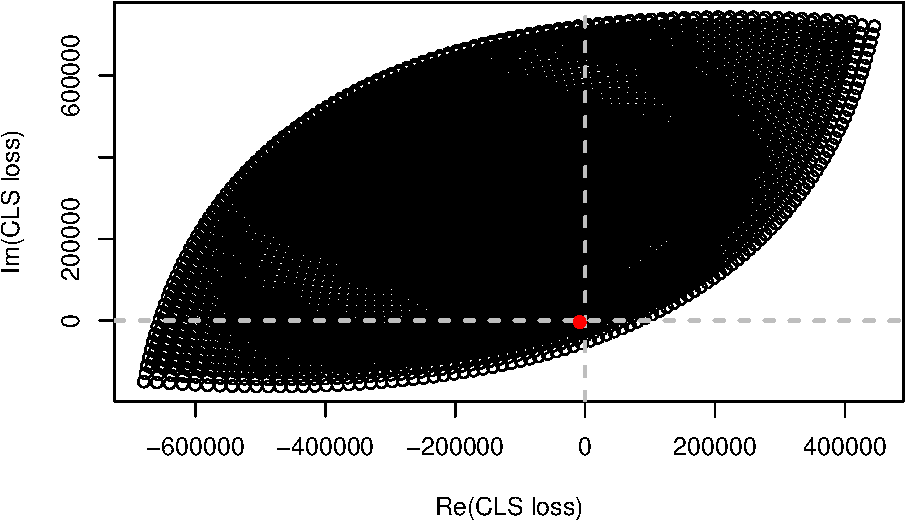
\includegraphics{Svetunkov---Svetunkov---Complex-Valued-Econometrics_files/figure-latex/clsScatter-1.pdf}
\caption{\label{fig:clsScatter}Variety of CLS loss function values for different values of \(\underline{b}_1\).}
\end{figure}

Figure \ref{fig:clsScatter} shows a scatterplot of values of the complex loss \eqref{eq:SimpleCLRCLSLoss}. The red point close to the origin corresponds to the estimate obtained using \eqref{eq:SimpleCLRCLSLossParametersMoments}. As we can see, it is close to the origin, which implies that the minimisation of the loss \eqref{eq:SimpleCLRCLSLoss} is equivalent to making both real and imaginary parts of it close to zero. This means that CLS makes variances of real and imaginary residuals similar and shrinks the covariance between them to zero.

Another way of looking at how CLS works is to reduce its dimensionality via the Multidimensional Scaling \citep{Gower} and then visualise it. The R code below is relatively slow but produces a solution for this task.

\begin{Shaded}
\begin{Highlighting}[]
\CommentTok{\# Calculate distance matrix for all losses}
\CommentTok{\# (including the CLS point)}
\NormalTok{clsMDSDistance \textless{}{-}}\StringTok{ }\KeywordTok{dist}\NormalTok{(}\KeywordTok{rbind}\NormalTok{(clsValues[,}\DecValTok{3}\OperatorTok{:}\DecValTok{4}\NormalTok{],}
                             \KeywordTok{c}\NormalTok{(}\KeywordTok{Re}\NormalTok{(clsResult),}\KeywordTok{Im}\NormalTok{(clsResult))))}

\CommentTok{\# Do Multidimensional scaling}
\NormalTok{clsMDS \textless{}{-}}\StringTok{ }\KeywordTok{cmdscale}\NormalTok{(clsMDSDistance, }\DataTypeTok{k=}\DecValTok{1}\NormalTok{)}

\CommentTok{\# Create a data frame with the coordinates}
\NormalTok{clsMDSValues \textless{}{-}}\StringTok{ }\KeywordTok{data.frame}\NormalTok{(}\DataTypeTok{z=}\NormalTok{clsMDS,}
                           \DataTypeTok{x=}\KeywordTok{c}\NormalTok{(clsValues[,}\DecValTok{1}\NormalTok{],}\KeywordTok{Re}\NormalTok{(bOptimal)),}
                           \DataTypeTok{y=}\KeywordTok{c}\NormalTok{(clsValues[,}\DecValTok{2}\NormalTok{],}\KeywordTok{Im}\NormalTok{(bOptimal)))}

\CommentTok{\# Create a matrix with loss values for 3d plotting}
\NormalTok{clsMDSValuesZ \textless{}{-}}\StringTok{ }\KeywordTok{matrix}\NormalTok{(clsMDSValues}\OperatorTok{$}\NormalTok{z[}\OperatorTok{{-}}\DecValTok{10001}\NormalTok{], }\DecValTok{100}\NormalTok{, }\DecValTok{100}\NormalTok{)}
\end{Highlighting}
\end{Shaded}

Then, to produce the 3d surface on the plane of "loss - \(b_{1,r}\) - \(b_{1,i}\), we can use functions from the \texttt{plotly} package in R as shown in the code below:

\begin{Shaded}
\begin{Highlighting}[]
\KeywordTok{plot\_ly}\NormalTok{(}\DataTypeTok{z=}\NormalTok{clsMDSValuesZ,}
        \DataTypeTok{x=}\KeywordTok{unique}\NormalTok{(clsMDSValues}\OperatorTok{$}\NormalTok{x[}\OperatorTok{{-}}\DecValTok{10001}\NormalTok{]),}
        \DataTypeTok{y=}\KeywordTok{unique}\NormalTok{(clsMDSValues}\OperatorTok{$}\NormalTok{y[}\OperatorTok{{-}}\DecValTok{10001}\NormalTok{])) }\OperatorTok{|}\ErrorTok{\textgreater{}}
\StringTok{    }\NormalTok{plotly}\OperatorTok{::}\KeywordTok{layout}\NormalTok{(}\DataTypeTok{scene=}\KeywordTok{list}\NormalTok{(}\DataTypeTok{xaxis =} \KeywordTok{list}\NormalTok{(}\DataTypeTok{title =} \StringTok{"Re(b1)"}\NormalTok{),}
                      \DataTypeTok{yaxis =} \KeywordTok{list}\NormalTok{(}\DataTypeTok{title =} \StringTok{"Im(b1)"}\NormalTok{),}
                      \DataTypeTok{zaxis =} \KeywordTok{list}\NormalTok{(}\DataTypeTok{title =} \StringTok{"MDS of CLS loss"}\NormalTok{))) }\OperatorTok{|}\ErrorTok{\textgreater{}}
\StringTok{    }\KeywordTok{add\_surface}\NormalTok{() }\OperatorTok{|}\ErrorTok{\textgreater{}}
\StringTok{    }\KeywordTok{add\_trace}\NormalTok{(}\DataTypeTok{data =} \KeywordTok{tail}\NormalTok{(clsMDSValues,}\DecValTok{1}\NormalTok{),}
              \DataTypeTok{x =} \OperatorTok{\textasciitilde{}}\NormalTok{x,}
              \DataTypeTok{y =} \OperatorTok{\textasciitilde{}}\NormalTok{y,}
              \DataTypeTok{z =} \OperatorTok{\textasciitilde{}}\NormalTok{z,}
              \DataTypeTok{mode =} \StringTok{"markers"}\NormalTok{,}
              \DataTypeTok{type =} \StringTok{"scatter3d"}\NormalTok{,}
              \DataTypeTok{marker =} \KeywordTok{list}\NormalTok{(}\DataTypeTok{size =} \DecValTok{10}\NormalTok{))}
\end{Highlighting}
\end{Shaded}

\begin{figure}
\centering
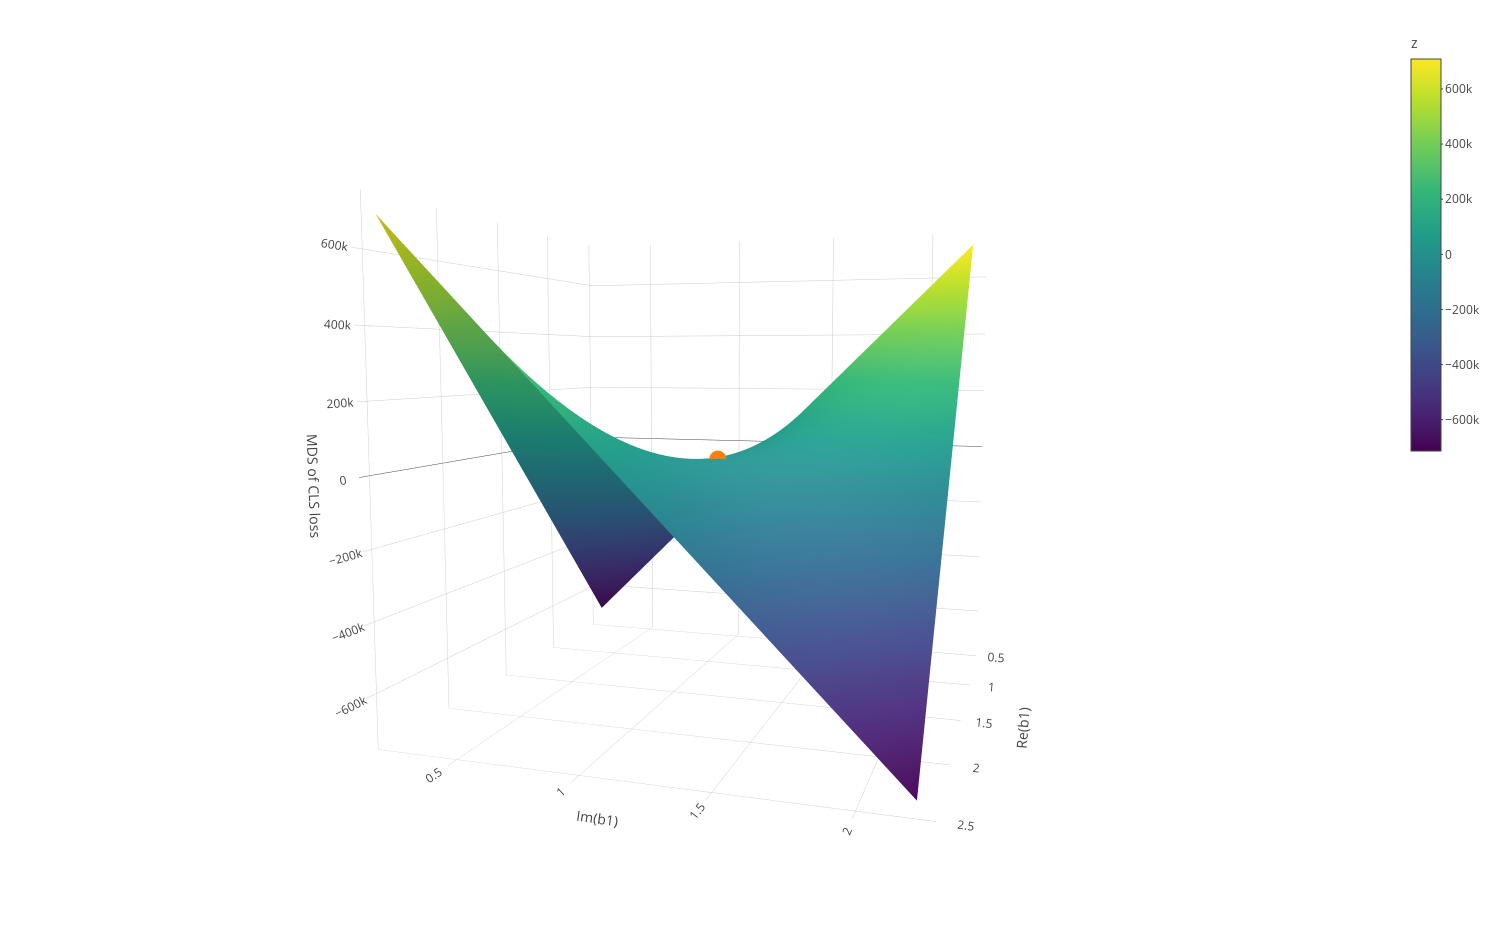
\includegraphics{images/CLSPlot.png}
\caption{\label{fig:plotlyCLS}Plot of the 3d surface for the MDS of the CLS loss.}
\end{figure}

Figure \ref{fig:plotlyCLS} demonstrates how the projection of the two-dimensional loss behaves for a variety of parameters of the regression. The orange point in the middle corresponds to the one obtained via CLS. We can see that it corresponds to the loss being close to zero, and represents a 2-dimensional inflection point, where the surface bends in different directions.

So, we can see that despite being counter-intuitive, the CLS produces the estimates of parameters that lead to the residuals being close to spherical (normal if we assume normality), because the variances of real and imaginary parts of the residuals become closer to each other, while the covariance between them becomes close to zero.

\hypertarget{SCLREstimationLikelihood}{%
\subsection{Likelihood}\label{SCLREstimationLikelihood}}

Finally, another way of estimating the simple cLR is by assuming a distribution of the residuals and maximising the respective likelihood. Given the connection between the linear and the vector forms of the complex regression, we can assume that the error term follows a multivariate normal distribution with a covariance matrix:
\begin{equation}
    \boldsymbol{\Sigma}_\epsilon = \begin{pmatrix} \sigma_{\epsilon_r}^2 & \sigma_{\epsilon_r, \epsilon_i} \\ \sigma_{\epsilon_r, \epsilon_i} & \sigma_{\epsilon_i}^2 \end{pmatrix} .
    \label{eq:SimpleCLRLikelihoodSigma}
\end{equation}
The log-likelihood in this case can be written as:
\begin{equation}
    \ell(\boldsymbol{\theta}, \boldsymbol{\Sigma}_\epsilon | \mathbf{Y}) = -\frac{n}{2} \left( 2 \log(2 \pi) + \log | \boldsymbol{\Sigma}_\epsilon| \right) -\frac{1}{2} \sum_{j=1}^n \left( \boldsymbol{\epsilon}_j^\prime \boldsymbol{\Sigma}_\epsilon^{-1} \boldsymbol{\epsilon}_j \right) ,
    \label{eq:additiveLogLik}
\end{equation}
where \(\boldsymbol{\theta}\) is the vector of estimated parameters and \(\boldsymbol{\epsilon}_j = \begin{pmatrix} \epsilon_{r,j} \\ \epsilon_{i,j} \end{pmatrix}\) is the two dimensional error term. This likelihood is maximised when the covariance matrix \eqref{eq:SimpleCLRLikelihoodSigma} is estimated via:
\begin{equation}
    \hat{\boldsymbol{\Sigma}}_\epsilon = \frac{1}{n} \sum_{j=1}^{n} \boldsymbol{e}_j \boldsymbol{e}_j^\prime .
    \label{eq:Sigmaest}
\end{equation}
It can be shown that if the \eqref{eq:Sigmaest} is inserted in \eqref{eq:additiveLogLik} then the following concentrated log-likelihood can be obtained \citep[see, for example,][]{Snyder2017}:
\begin{equation}
    \ell^*(\boldsymbol{\theta}, \hat{\boldsymbol{\Sigma}}_\epsilon | \mathbf{Y}) = -\frac{n}{2} \left( 2 \log(2 \pi e) + \log | \hat{\boldsymbol{\Sigma}}_\epsilon | \right) .
    \label{eq:additiveLogLikConcentrated}
\end{equation}
It is obvious that the maximisation of the log-likelihood \eqref{eq:additiveLogLikConcentrated} is equivalent to minimising the generalised variance of the complex error term (as discussed in Subsection \ref{crvSecondMoment}):
\begin{equation}
    \mathrm{GV} = |\hat{\boldsymbol{\Sigma}}_\epsilon| = \sigma_{\epsilon_r}^2 \sigma_{\epsilon_i}^2 - \sigma_{\epsilon_r, \epsilon_i}^2 .
    \label{eq:additiveLogLikConcentratedGV}
\end{equation}
The minimisation of GV in its turn implies the joint minimisation of variances of the real and imaginary part of the residuals and a maximisation of the square of the covariance between them, thus making the residuals more linearly related. This loss function might be especially useful if we indeed can assume that the real and imaginary part of the residuals are linearly related and we want to use this information in the estimation.

The main difference between the Likelihood and the other two estimators discussed in this Section is that the former can only be maximised via a numeric optimisation - there is no analytical solution for estimates of parameters via likelihood.

\hypertarget{SCLREstimatorsComparison}{%
\section{Comparing different estimators for SCLR}\label{SCLREstimatorsComparison}}

Arguably, all three estimators discussed in this Section give adequate estimates of parameters, but inevitably they will have different efficiency and would be appropriate in different situations. In this subsection, we will explore the performance of estimators with the increase of sample size.

First, comparing variances of OLS and CLS estimates of \(b_{1,r}\) \eqref{eq:SimpleCLRCLSb1Variance} with \eqref{eq:SimpleCLROLSb1Variance}:
\begin{equation*}
    \begin{aligned}
        \mathrm{V}(b_{1,r}^{\mathrm{OLS}}) = & \mathrm{V}\left(\frac{\hat{\sigma}_{x_r, \epsilon_r} + \hat{\sigma}_{x_i, \epsilon_i}}{\hat{\sigma}_{x_r}^2 + \hat{\sigma}_{x_i}^2}\right) \\
        \mathrm{V}(b_{1,r}^{\mathrm{CLS}}) = & \mathrm{V}\left(\frac{\left(\hat{\sigma}_{x_r, \epsilon_r} - \hat{\sigma}_{x_i, \epsilon_i}\right) \left(\hat{\sigma}_{x_r}^2 - \hat{\sigma}_{x_i}^2 \right) - 2 \hat{\sigma}_{x_r, x_i} \left(\hat{\sigma}_{x_r, \epsilon_i} + \hat{\sigma}_{x_i, \epsilon_r}\right)}{\left(\hat{\sigma}_{x_r}^2 - \hat{\sigma}_{x_i}^2\right)^2 + 4 \hat{\sigma}_{x_r, x_i}^2}\right)
    \end{aligned}
\end{equation*}
we can conclude that there are some situations, when the estimates of parameters via CLS are less efficient than the estimates via OLS. There are some cases, when the variance \eqref{eq:SimpleCLRCLSb1Variance} is much higher than \eqref{eq:SimpleCLROLSb1Variance}. For example, when the real and imaginary parts of \(x\) are not correlated (i.e.~\(\hat{\sigma}_{x_r, x_i}=0\)) and when the variances of the real and imaginary parts of \(x\) are equal, the variance of \(b_{1,r}\) explodes. However, there are also some cases, when CLS estimates are more efficient than the OLS ones. For example, when \(\hat{\sigma}_{x_r, \epsilon_i}=\hat{\sigma}_{x_i, \epsilon_i}\) and \(\hat{\sigma}_{x_r, x_i}=0\), the variance \eqref{eq:SimpleCLROLSb1Variance} will be equal to zero, while the variance \eqref{eq:SimpleCLRCLSb1Variance} will be greater than zero. So, in general, we cannot conclude which of the estimators will be more efficient, but we know that in different circumstances, they will have different properties.

We cannot compare the efficiency of the likelihood estimator directly with the OLS and CLS, but we know from the statistics literature \citep{referenceLikelihoodPaper} that likelihood gives consistent and asymptotically efficient estimates of parameters.

In terms of consistency, in one specific situation, when \(\hat{\sigma}_{x_r}^2 = \hat{\sigma}_{x_i}^2\) and \(\hat{\sigma}_{x_r, x_i}=0\), CLS might produce non-consistent estimates of parameters. This means that if we deal with explanatory variables with these properties, we should use either OLS or Likelihood.

Similar analysis can be done for the coefficient \(b_{1,i}\), with the conclusions similar to the above, so we skip this discussion.

In order to do a more thorough comparison of the three estimators, we set up an experiment based on the following simple cLR:
\begin{equation*}
    y_r + i y_i = 10+15i + (2-1.5i) (x_r + i x_i) + (\epsilon_r + i \epsilon_i)
\end{equation*}
with several scenarios, parameters for which are shown in Table \ref{tab:scenariosEstimators}. They covered several important situations: when \(x_r\) and \(x_i\) are not correlated, have medium correlation and perfectly correlated, when their variances are similar or different and then when the real and imaginary parts of the error term are not correlated, have medium correlation, are equal to zero and when their variances have high or low values.

\begin{table}

\caption{\label{tab:scenariosEstimators}Several scenarios for the comparison of estimators.}
\centering
\resizebox{\linewidth}{!}{
\fontsize{12}{14}\selectfont
\begin{tabular}[t]{l|l|l|l|l}
\hline
  & cor($x_r$, $x_i$) & std.dev. of $x_r$ and $x_i$ & cor($\epsilon_r$, $\epsilon_i$) & std.dev. of $\epsilon_r$ and $\epsilon_i$\\
\hline
Scenario 1 & 0 & $\sigma_{x_r}=10$, $\sigma_{x_i}=20$ & 0 & $\sigma_{\epsilon_r}=\sigma_{\epsilon_i}=1.5$\\
\hline
Scenario 2 & 1 & $\sigma_{x_r}=10$, while $\sigma_{x_i}=15$ & 0 & $\sigma_{\epsilon_r}=\sigma_{\epsilon_i}=1.5$\\
\hline
Scenario 3 & 0 & $\sigma_{x_r}=\sigma_{x_i}=20$ & 0 & $\sigma_{\epsilon_r}=\sigma_{\epsilon_i}=1.5$\\
\hline
Scenario 4 & medium & $\sigma_{x_r}=10$, $\sigma_{x_i}=15$ & NA & $\sigma_{\epsilon_r}=\sigma_{\epsilon_i}=0$\\
\hline
Scenario 5 & medium & $\sigma_{x_r}=10$, $\sigma_{x_i}=15$ & medium & $\sigma_{\epsilon_r}=10$, $\sigma_{\epsilon_i}=8$\\
\hline
Scenario 6 & medium & $\sigma_{x_r}=10$, $\sigma_{x_i}=15$ & 0 & $\sigma_{\epsilon_r}=\sigma_{\epsilon_i}=100$\\
\hline
\end{tabular}}
\end{table}

These six scenarios in Table \ref{tab:scenariosEstimators} cover different theoretically possible situations and show how the three estimators behave in these conditions. The sample size was first set to 20 observations and then was increased iteratively by one observation until reaching 10,000. This should give us an understanding of how the estimators behave both on small samples and asymptotically. While we recorded both values of estimated intercept and slope, we are mainly interested in the latter, and the plots shown below focus on how the complex \(\underline{b}_1\) is estimated. The experiments were done using \texttt{clm()} function from the \texttt{complex} package with \texttt{method} parameter equal to ``OLS'', ``CLS'' and ``likelihood'' for each of the respective estimators. A sample of the script used in the experiments is shown below (Scenario 1):

\begin{Shaded}
\begin{Highlighting}[]
\NormalTok{obs \textless{}{-}}\StringTok{ }\DecValTok{10000}
\NormalTok{x0 \textless{}{-}}\StringTok{ }\KeywordTok{rnorm}\NormalTok{(obs,}\DecValTok{10}\NormalTok{,}\DecValTok{10}\NormalTok{)}
\NormalTok{x \textless{}{-}}\StringTok{ }\KeywordTok{complex}\NormalTok{(}\DataTypeTok{real=}\NormalTok{x0,}\DataTypeTok{imaginary=}\KeywordTok{rnorm}\NormalTok{(obs,}\DecValTok{0}\NormalTok{,}\DecValTok{20}\NormalTok{))}

\NormalTok{b0 \textless{}{-}}\StringTok{ }\DecValTok{10} \OperatorTok{+}\StringTok{ }\NormalTok{15i}
\NormalTok{b1 \textless{}{-}}\StringTok{ }\DecValTok{2}\FloatTok{{-}1.5}\NormalTok{i}
\NormalTok{y \textless{}{-}}\StringTok{ }\NormalTok{b0 }\OperatorTok{+}\StringTok{ }\NormalTok{b1 }\OperatorTok{*}\StringTok{ }\NormalTok{x }\OperatorTok{+}\StringTok{ }\FloatTok{1.5}\OperatorTok{*}\KeywordTok{complex}\NormalTok{(}\DataTypeTok{real=}\KeywordTok{rnorm}\NormalTok{(obs,}\DecValTok{0}\NormalTok{,}\DecValTok{1}\NormalTok{),}
                               \DataTypeTok{imaginary=}\KeywordTok{rnorm}\NormalTok{(obs,}\DecValTok{0}\NormalTok{,}\DecValTok{1}\NormalTok{))}

\NormalTok{complexData \textless{}{-}}\StringTok{ }\KeywordTok{cbind}\NormalTok{(y,x)}

\NormalTok{nsim \textless{}{-}}\StringTok{ }\DecValTok{9980}
\NormalTok{parametersValues \textless{}{-}}
\StringTok{    }\KeywordTok{array}\NormalTok{(}\OtherTok{NA}\NormalTok{, }\KeywordTok{c}\NormalTok{(nsim,}\DecValTok{3}\NormalTok{,}\DecValTok{2}\NormalTok{),}
          \DataTypeTok{dimnames=}\KeywordTok{list}\NormalTok{(}\OtherTok{NULL}\NormalTok{,}
                        \KeywordTok{c}\NormalTok{(}\StringTok{"CLS"}\NormalTok{,}\StringTok{"OLS"}\NormalTok{,}\StringTok{"Likelihood"}\NormalTok{),}
                        \KeywordTok{c}\NormalTok{(}\StringTok{"b0"}\NormalTok{,}\StringTok{"b1"}\NormalTok{)))}

\ControlFlowTok{for}\NormalTok{(i }\ControlFlowTok{in} \DecValTok{1}\OperatorTok{:}\NormalTok{nsim)\{}
\NormalTok{    test \textless{}{-}}\StringTok{ }\KeywordTok{clm}\NormalTok{(y}\OperatorTok{\textasciitilde{}}\NormalTok{x, complexData, }\DataTypeTok{loss=}\StringTok{"CLS"}\NormalTok{,}
                \DataTypeTok{subset=}\KeywordTok{sample}\NormalTok{(}\KeywordTok{c}\NormalTok{(}\DecValTok{1}\OperatorTok{:}\NormalTok{obs),}\DecValTok{20}\OperatorTok{+}\NormalTok{i))}
\NormalTok{    parametersValues[i,}\DecValTok{1}\NormalTok{,] \textless{}{-}}\StringTok{ }\KeywordTok{coef}\NormalTok{(test)}
\NormalTok{    test \textless{}{-}}\StringTok{ }\KeywordTok{clm}\NormalTok{(y}\OperatorTok{\textasciitilde{}}\NormalTok{x, complexData, }\DataTypeTok{loss=}\StringTok{"OLS"}\NormalTok{,}
                \DataTypeTok{subset=}\KeywordTok{sample}\NormalTok{(}\KeywordTok{c}\NormalTok{(}\DecValTok{1}\OperatorTok{:}\NormalTok{obs),}\DecValTok{20}\OperatorTok{+}\NormalTok{i))}
\NormalTok{    parametersValues[i,}\DecValTok{2}\NormalTok{,] \textless{}{-}}\StringTok{ }\KeywordTok{coef}\NormalTok{(test)}
\NormalTok{    test \textless{}{-}}\StringTok{ }\KeywordTok{clm}\NormalTok{(y}\OperatorTok{\textasciitilde{}}\NormalTok{x, complexData, }\DataTypeTok{loss=}\StringTok{"likelihood"}\NormalTok{,}
                \DataTypeTok{subset=}\KeywordTok{sample}\NormalTok{(}\KeywordTok{c}\NormalTok{(}\DecValTok{1}\OperatorTok{:}\NormalTok{obs),}\DecValTok{20}\OperatorTok{+}\NormalTok{i))}
\NormalTok{    parametersValues[i,}\DecValTok{3}\NormalTok{,] \textless{}{-}}\StringTok{ }\KeywordTok{coef}\NormalTok{(test)}
\NormalTok{\}}
\end{Highlighting}
\end{Shaded}

Figure \ref{fig:parametersUCDV} demonstrates how estimates of parameters change with the increase of sample size in Scenario 1.

\begin{figure}
\centering
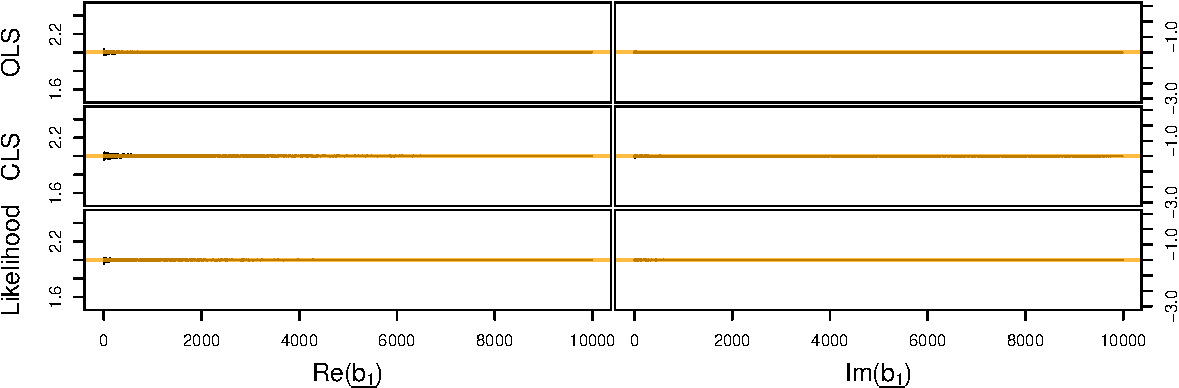
\includegraphics{Svetunkov---Svetunkov---Complex-Valued-Econometrics_files/figure-latex/parametersUCDV-1.pdf}
\caption{\label{fig:parametersUCDV}Estimation of parameters using OLS, CLS and likelihood and their convergence to the true value of \(\underline{\beta_1}=2-1.5i\) (orange horizontal lines on the plot). Scenario 1.}
\end{figure}

Apparently, all three estimators produce very similar estimates of parameters in this case and converge to the true values quite fast. A similar behaviour is observed for the Scenario 2, shown in Figure \ref{fig:parametersPC}. The difference between the three estimators does not look substantial.

\begin{figure}
\centering
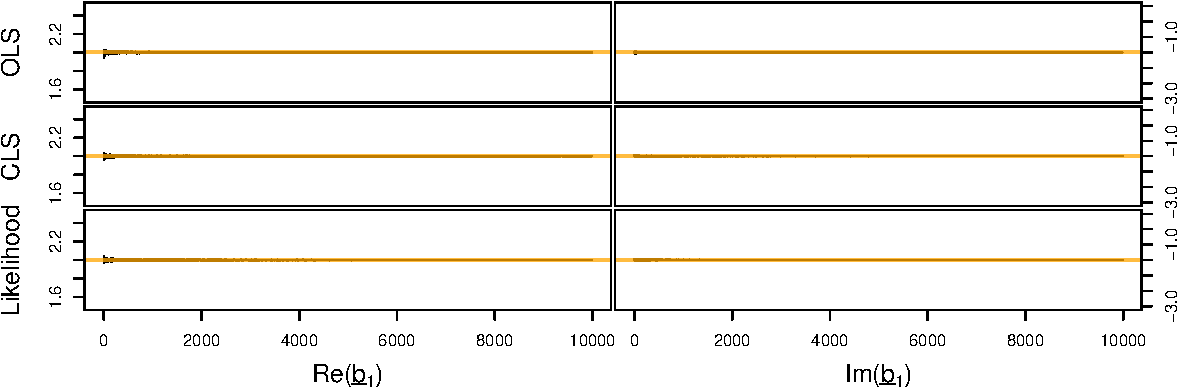
\includegraphics{Svetunkov---Svetunkov---Complex-Valued-Econometrics_files/figure-latex/parametersPC-1.pdf}
\caption{\label{fig:parametersPC}Estimation of parameters using OLS, CLS and likelihood and their convergence to the true value of \(\underline{\beta_1}=2-1.5i\) (orange horizontal lines on the plot). Scenario 2.}
\end{figure}

In both Scenarios 1 and 2 the error term has a small variance, in Scenario 2 \(x_r\) and \(x_i\) are perfectly correlated, transforming the original model into: \(y_r + i y_i = 10+15i + (2-1.5i) (1 + 1.5 i) x_r + (\epsilon_r + i \epsilon_i)\).

The Scenario 3 demonstrates an exotic case, when the variances of \(x_r\) and \(x_i\) are the same (as shown in Figure \ref{fig:parametersUCSV}).

\begin{figure}
\centering
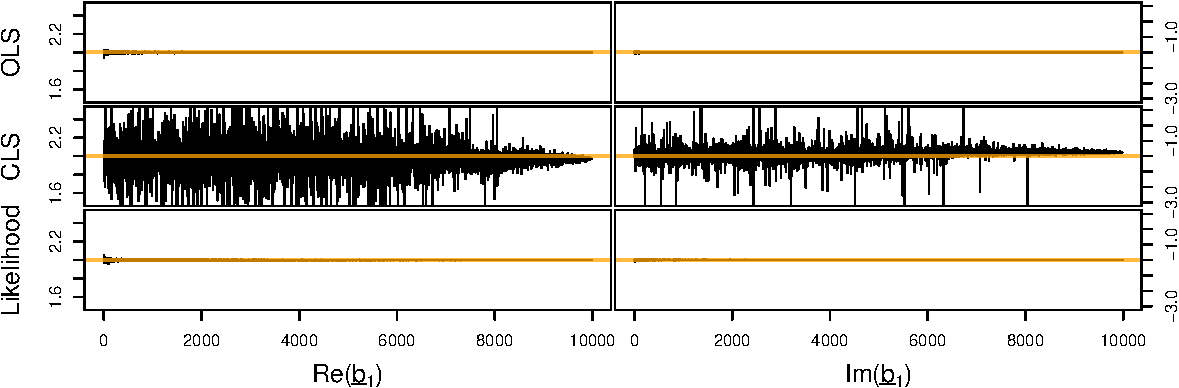
\includegraphics{Svetunkov---Svetunkov---Complex-Valued-Econometrics_files/figure-latex/parametersUCSV-1.pdf}
\caption{\label{fig:parametersUCSV}Estimation of parameters using OLS, CLS and likelihood and their convergence to the true value of \(\underline{\beta_1}=2-1.5i\) (orange horizontal lines on the plot). Scenario 3.}
\end{figure}

In this scenario, OLS and Likelihood produce efficient, unbiased and consistent estimates of parameters, which cannot be said about the CLS. The behaviour of CLS is explainable because for this specific scenario the direct variance of the complex variable \(x_r + i x_i\) becomes close to zero. As a result, the direct covariance in \eqref{eq:SimpleCLRCLSLossParametersMomentsExpanded} is divided by zero, and the estimate of the parameter becomes unstable. Scenarios 1 and 3 could be considered as two special cases of the spectrum of values, showing that the closer the variances of the real and imaginary parts of \(x\) are, the less consistent, efficient and unbiased estimates of parameters are produced by CLS. Scenario 2 is complimentary, because it shows that if the real and imaginary parts are correlated, the CLS estimates of parameters become as good (in statistical terms) as the estimates of OLS and/or Likelihood. So, the CLS becomes unreliable in a special case, when \(\sigma_{x_r}^2 = \sigma_{x_i}^2\) and \(\sigma_{x_r,x_i}=0\).

Next, the three estimators give the same estimates of parameters in Scenario 4 of functional relation between \(x\) and \(y\), which is shown in Figure \ref{fig:parametersFR}.

\begin{figure}
\centering
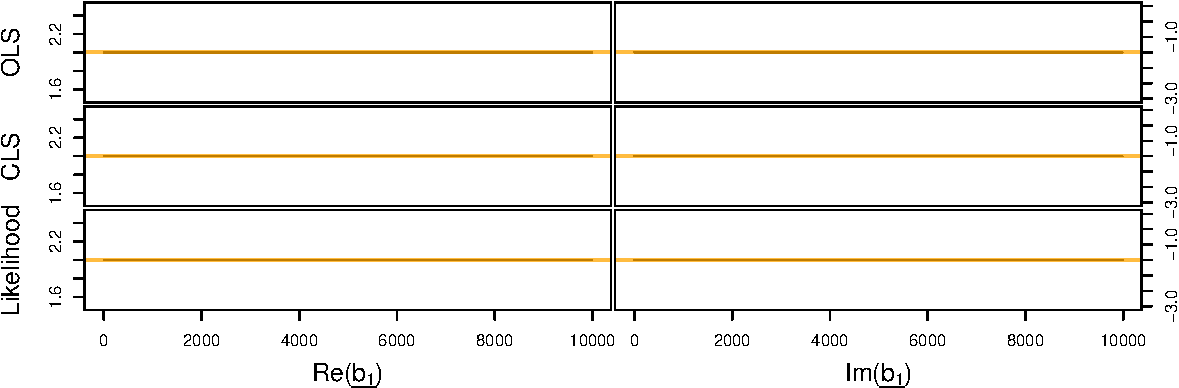
\includegraphics{Svetunkov---Svetunkov---Complex-Valued-Econometrics_files/figure-latex/parametersFR-1.pdf}
\caption{\label{fig:parametersFR}Estimation of parameters using OLS, CLS and likelihood and their convergence to the true value of \(\underline{\beta_1}=2-1.5i\) (orange horizontal lines on the plot). Scenario 4.}
\end{figure}

The main difficulties for the estimators appear, when the variance of the error term increases. Figure \ref{fig:parametersCorError} shows how the three perform in case of a higher variance of the error term in Scenario 5.

\begin{figure}
\centering
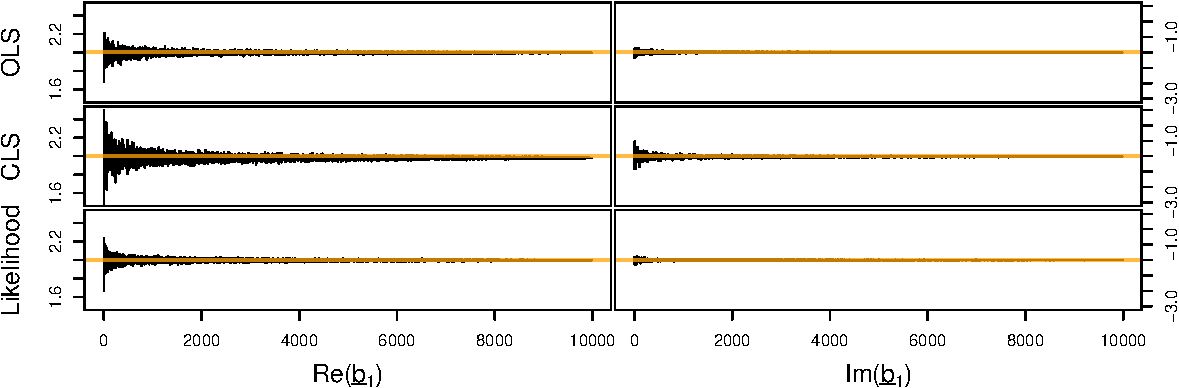
\includegraphics{Svetunkov---Svetunkov---Complex-Valued-Econometrics_files/figure-latex/parametersCorError-1.pdf}
\caption{\label{fig:parametersCorError}Estimation of parameters using OLS, CLS and likelihood and their convergence to the true value of \(\underline{\beta_1}=2-1.5i\) (orange horizontal lines on the plot). Scenario 5.}
\end{figure}

It becomes apparent that OLS and Likelihood produce more efficient estimates of parameters than CLS on small samples. This is because the variability of estimates of parameter is higher for CLS than for the other two on small samples.

The situations worsens for the three estimators when we consider Scenario 6, when the variances of the error term become much higher than before, which is shown in Figure \ref{fig:parametersHVError}.

\begin{figure}
\centering
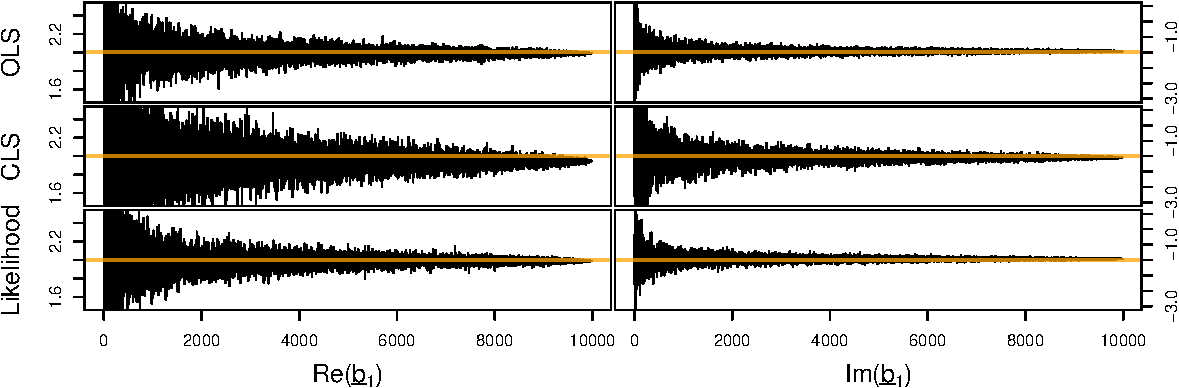
\includegraphics{Svetunkov---Svetunkov---Complex-Valued-Econometrics_files/figure-latex/parametersHVError-1.pdf}
\caption{\label{fig:parametersHVError}Estimation of parameters using OLS, CLS and likelihood and their convergence to the true value of \(\underline{\beta_1}=2-1.5i\) (orange horizontal lines on the plot). Scenario 6.}
\end{figure}

In addition to being less efficient, the real parts of estimates of parameters exhibit a bias, which is diminished with the increase of sample size. Comparing the three estimators, it appears that CLS produces less efficient and more biased estimates of parameters than OLS or Likelihood in this Scenario.

These six scenarios show a variety of situations in which the three estimators produce different estimates of parameters. Arguably, OLS and Likelihood could be considered as robust alternatives, but all the three estimators seem to perform well in several sensible situations.

\hypertarget{correlationAnalysis}{%
\chapter{Correlation analysis of complex random variables}\label{correlationAnalysis}}

When it comes to measuring associations between variables, most frequently analysts use coefficient of correlation. While it is straightforward for real-valued variables, for complex variables this become challenging, because each c.r.v. has two parts, so the correlation needs to take them both into account.

For modelling purposes, it might be useful to have the information about all possible correlations involved relation of two c.r.v. This comes to analysing the following covariances for variables \(\underline{x}\) and \(\underline{y}\):

\begin{enumerate}
\def\labelenumi{\arabic{enumi}.}
\tightlist
\item
  \(\sigma_{x_r,x_i}\),
\item
  \(\sigma_{y_r,y_i}\),
\item
  \(\sigma_{x_r,y_r}\),
\item
  \(\sigma_{x_i,y_i}\),
\item
  \(\sigma_{x_r,y_i}\),
\item
  \(\sigma_{y_r,x_i}\).
\end{enumerate}

\hypertarget{correlationVisual}{%
\section{Visualisation of relations}\label{correlationVisual}}

In order to better understand what correlations between c.r.v. imply, we need to understand how to produce scatterplots for them. While in case of two real variables it is straightforward (a variable per axes), in our situation, this becomes challenging. We propose considering a set of scatterplots shown in Figure \ref{fig:crvScatterplots} for two generated complex random variables \(\underline{x}\) and \(\underline{y}\), created using \texttt{cplot()} function from \texttt{complex} package in R.

\begin{Shaded}
\begin{Highlighting}[]
\CommentTok{\# Create real part of a c.r.v. x}
\NormalTok{xr \textless{}{-}}\StringTok{ }\KeywordTok{rnorm}\NormalTok{(}\DecValTok{1000}\NormalTok{,}\DecValTok{0}\NormalTok{,}\DecValTok{10}\NormalTok{)}
\CommentTok{\# Create a c.r.v. x}
\NormalTok{x \textless{}{-}}\StringTok{ }\KeywordTok{complex}\NormalTok{(}\DataTypeTok{real=}\NormalTok{xr, }\DataTypeTok{imaginary=}\FloatTok{1.5}\OperatorTok{*}\NormalTok{xr}\OperatorTok{+}\KeywordTok{rnorm}\NormalTok{(}\DecValTok{1000}\NormalTok{,}\DecValTok{0}\NormalTok{,}\DecValTok{10}\NormalTok{))}
\CommentTok{\# Create a c.r.v. y}
\NormalTok{y \textless{}{-}}\StringTok{ }\NormalTok{(}\DecValTok{10} \OperatorTok{+}\StringTok{ }\NormalTok{15i) }\OperatorTok{+}\StringTok{ }\NormalTok{(}\FloatTok{1.5} \OperatorTok{+}\StringTok{ }\FloatTok{1.2}\NormalTok{i) }\OperatorTok{*}\StringTok{ }\NormalTok{x }\OperatorTok{+}
\StringTok{    }\KeywordTok{complex}\NormalTok{(}\DataTypeTok{real=}\KeywordTok{rnorm}\NormalTok{(}\DecValTok{1000}\NormalTok{,}\DecValTok{0}\NormalTok{,}\DecValTok{10}\NormalTok{), }\DataTypeTok{imaginary=}\KeywordTok{rnorm}\NormalTok{(}\DecValTok{1000}\NormalTok{,}\DecValTok{0}\NormalTok{,}\DecValTok{10}\NormalTok{))}
\CommentTok{\# Produce the plot}
\KeywordTok{cplot}\NormalTok{(x, y, }\DataTypeTok{which=}\DecValTok{1}\NormalTok{)}
\end{Highlighting}
\end{Shaded}

\begin{figure}
\centering
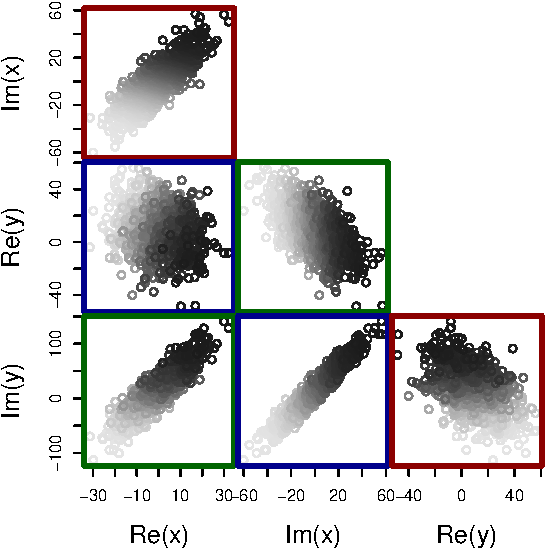
\includegraphics{Svetunkov---Svetunkov---Complex-Valued-Econometrics_files/figure-latex/crvScatterplots-1.pdf}
\caption{\label{fig:crvScatterplots}Visualisation of relations between two complex variables}
\end{figure}

This scatterplot has several important elements in it:

\begin{itemize}
\tightlist
\item
  It shows relations between real and imaginary parts of each variable (e.g.~the two scatterplots in the bold dark red frame),
\item
  It shows cross-relations between parts of one variable and parts of the other one (e.g.~the rest four plots),
\item
  The colour shows ordering of the original variable \(\underline{x}\) with dark values corresponding to point with higher magnitude and light ones being closer to zero. This way, we can see what the original points in \(\underline{x}\) correspond to in \(\underline{y}\).
\end{itemize}

The plots are positioned to satisfy two rules:

\begin{enumerate}
\def\labelenumi{\arabic{enumi}.}
\tightlist
\item
  When a scatterplot for a c.r.v. is produced, the real part should be in x-axis, while the imaginary should be in the y-axis.
\item
  When parts of variables \(\underline{x}\) and \(\underline{y}\) are compared, the part for \(\underline{x}\) should be in x-axis, while the part for \(\underline{y}\) should be in y-axis, which should the reflect the idea that \(\underline{x}\) could be an explanatory variable for \(\underline{y}\).
\end{enumerate}

While a simple scatterplot matrix could have been constructed instead of Figure \ref{fig:crvScatterplots}, we argue that the latter has a logical grouping and should be preferred for analysis of complex variables. For example, based on the plots in Figure \ref{fig:crvScatterplots} we can conclude that:

\begin{itemize}
\tightlist
\item
  There is a positive relation between the real and imaginary parts of \(\underline{x}\),
\item
  There is a negative relation between the real and imaginary parts of \(\underline{y}\),
\item
  Real parts of \(\underline{x}\) and \(\underline{y}\) do not exhibit a strong linear relation,
\item
  But the respective imaginary parts of \(\underline{x}\) and \(\underline{y}\) have the positive relation between them,
\item
  Finally, we see that with the increase of real and imaginary parts of \(\underline{x}\), the real part of \(\underline{y}\) decreases, while the imaginary one increases. This sort of behaviour implies positive complex slope in the potential linear regression (discussed in Section \ref{simpleCLR}).
\end{itemize}

We think that this visualisation is useful when analysing relations between two complex random variables. But it also shows how complicated it is to capture the relation between them and how many aspects need to be considered.

As an alternative to the plot above, it is also possible to use some dimensionality reduction techniques to plot complex variables on a two dimensional plot. For example, we can use Multidimensional Scaling for this \citep[MDS,][]{refMDS} to create a project of one complex variable on x-axis and another one on the y-axis. In R, we can use the \texttt{cmdscale()} function from \texttt{stats} package for this (in the example below, we use euclidean distance for the dissimilarities matrix via \texttt{dist()} function from \texttt{stats}, and we use the \texttt{complex2vec()} function from \texttt{complex} package to transform complex variable to a collection of vectors):

\begin{Shaded}
\begin{Highlighting}[]
\KeywordTok{complex2vec}\NormalTok{(x) }\OperatorTok{|}\ErrorTok{\textgreater{}}\StringTok{ }\KeywordTok{dist}\NormalTok{() }\OperatorTok{|}\ErrorTok{\textgreater{}}\StringTok{ }\KeywordTok{cmdscale}\NormalTok{(}\DataTypeTok{k=}\DecValTok{1}\NormalTok{) {-}\textgreater{}}\StringTok{ }\NormalTok{xScaled}
\KeywordTok{complex2vec}\NormalTok{(y) }\OperatorTok{|}\ErrorTok{\textgreater{}}\StringTok{ }\KeywordTok{dist}\NormalTok{() }\OperatorTok{|}\ErrorTok{\textgreater{}}\StringTok{ }\KeywordTok{cmdscale}\NormalTok{(}\DataTypeTok{k=}\DecValTok{1}\NormalTok{) {-}\textgreater{}}\StringTok{ }\NormalTok{yScaled}
\KeywordTok{plot}\NormalTok{(xScaled,yScaled)}
\end{Highlighting}
\end{Shaded}

The same code is implemented in \texttt{cplot()} function from \texttt{complex} package in R:

\begin{Shaded}
\begin{Highlighting}[]
\KeywordTok{cplot}\NormalTok{(x, y, }\DataTypeTok{which=}\DecValTok{2}\NormalTok{, }\DataTypeTok{main=}\StringTok{""}\NormalTok{)}
\end{Highlighting}
\end{Shaded}

\begin{figure}
\centering
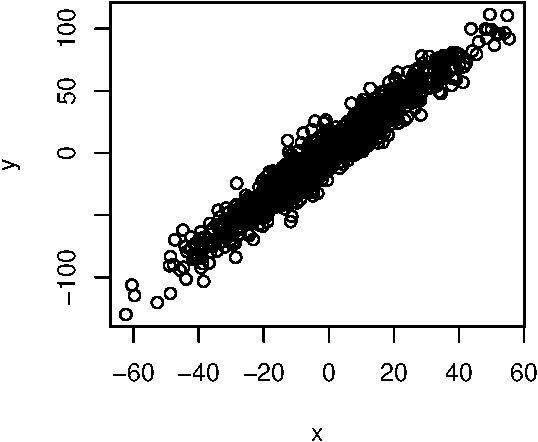
\includegraphics{Svetunkov---Svetunkov---Complex-Valued-Econometrics_files/figure-latex/crvScatterplotMDS-1.pdf}
\caption{\label{fig:crvScatterplotMDS}Scatterplot of MDS of two complex variables.}
\end{figure}

The plot in Figure \ref{fig:crvScatterplotMDS} is much easier to read than the collection of scatterplots in Figure \ref{fig:crvScatterplots}, and in our example, we can conclude that the two complex variables exhibit strong linear relation.

\hypertarget{correlationTypes}{%
\section{Types of correlation coefficients}\label{correlationTypes}}

The literature knows two correlation coefficients for complex variables \citep{ref}: the conjugate and the direct correlation (the latter is known in the literature as ``pseudo-correlation''). Their formula are based on the respective covariances and variances (conjugate and direct discussed in Subsection \ref{crvSecondMoment}):

\begin{enumerate}
\def\labelenumi{\arabic{enumi}.}
\item
  Conjugate correlation
  \begin{equation}
   \rho_{x,y} = \frac{\sqrt{\sigma_{x,y} \sigma_{y,x}}}{\sigma_x \sigma_y},
   \label{eq:correlationConjugate}
  \end{equation}
\item
  Direct correlation
  \begin{equation}
   \varrho_{x,y} = \frac{\varsigma_{x,y}}{\varsigma_x \varsigma_y}.
   \label{eq:correlationDirect}
  \end{equation}
\end{enumerate}

Note that the conjugate correlation has the geometric mean of standard deviations in the numerator. This is needed because of the issue with the conjugate covariance (its value changes with the change of conjugate number). If we use only one of covariances \citep[as done, for example, by][]{Panchev1971} then the value of correlation coefficient will be ambiguous, implying that the correlation between \(\underline{x}\) and \(\underline{y}\) differs from the correlation between \(\underline{y}\) and \(\underline{x}\). Furthermore, such correlation coefficient would not work as intended. For example, if we have a positive functional linear relation between \(\underline{x}\) and \(\underline{y}\), the coefficient should be equal to one. But as an R example below demonstrates this value is obtained only if we have the geometric mean of covariances.

\begin{Shaded}
\begin{Highlighting}[]
\NormalTok{x \textless{}{-}}\StringTok{ }\KeywordTok{complex}\NormalTok{(}\DataTypeTok{real=}\KeywordTok{rnorm}\NormalTok{(}\DecValTok{100}\NormalTok{,}\DecValTok{0}\NormalTok{,}\DecValTok{10}\NormalTok{), }\DataTypeTok{imaginary=}\KeywordTok{rnorm}\NormalTok{(}\DecValTok{100}\NormalTok{,}\DecValTok{0}\NormalTok{,}\DecValTok{10}\NormalTok{))}
\NormalTok{y \textless{}{-}}\StringTok{ }\NormalTok{(}\DecValTok{10} \OperatorTok{+}\StringTok{ }\NormalTok{15i) }\OperatorTok{+}\StringTok{ }\NormalTok{(}\DecValTok{1} \OperatorTok{+}\StringTok{ }\NormalTok{1i) }\OperatorTok{*}\StringTok{ }\NormalTok{x}
\CommentTok{\# Variant 1}
\KeywordTok{ccov}\NormalTok{(y,x,}\DataTypeTok{method=}\StringTok{"conj"}\NormalTok{) }\OperatorTok{/}
\StringTok{    }\KeywordTok{sqrt}\NormalTok{(}\KeywordTok{cvar}\NormalTok{(x,}\DataTypeTok{method=}\StringTok{"conj"}\NormalTok{)}\OperatorTok{*}\KeywordTok{cvar}\NormalTok{(y,}\DataTypeTok{method=}\StringTok{"conj"}\NormalTok{))}
\end{Highlighting}
\end{Shaded}

\begin{verbatim}
## [1] 0.7071068-0.7071068i
\end{verbatim}

\begin{Shaded}
\begin{Highlighting}[]
\CommentTok{\# Variant 2}
\KeywordTok{ccov}\NormalTok{(x,y,}\DataTypeTok{method=}\StringTok{"conj"}\NormalTok{) }\OperatorTok{/}
\StringTok{    }\KeywordTok{sqrt}\NormalTok{(}\KeywordTok{cvar}\NormalTok{(x,}\DataTypeTok{method=}\StringTok{"conj"}\NormalTok{)}\OperatorTok{*}\KeywordTok{cvar}\NormalTok{(y,}\DataTypeTok{method=}\StringTok{"conj"}\NormalTok{))}
\end{Highlighting}
\end{Shaded}

\begin{verbatim}
## [1] 0.7071068+0.7071068i
\end{verbatim}

\begin{Shaded}
\begin{Highlighting}[]
\CommentTok{\# Variant 3 (correct conjugate correlation)}
\KeywordTok{sqrt}\NormalTok{(}\KeywordTok{ccov}\NormalTok{(y,x,}\DataTypeTok{method=}\StringTok{"conj"}\NormalTok{)}\OperatorTok{*}\KeywordTok{ccov}\NormalTok{(x,y,}\DataTypeTok{method=}\StringTok{"conj"}\NormalTok{)) }\OperatorTok{/}
\StringTok{    }\KeywordTok{sqrt}\NormalTok{((}\KeywordTok{cvar}\NormalTok{(x,}\DataTypeTok{method=}\StringTok{"conj"}\NormalTok{)}\OperatorTok{*}\KeywordTok{cvar}\NormalTok{(y,}\DataTypeTok{method=}\StringTok{"conj"}\NormalTok{)))}
\end{Highlighting}
\end{Shaded}

\begin{verbatim}
## [1] 1+0i
\end{verbatim}

\begin{Shaded}
\begin{Highlighting}[]
\CommentTok{\# Same thing using the ccor() function}
\KeywordTok{ccor}\NormalTok{(x,y,}\DataTypeTok{method=}\StringTok{"conjugate"}\NormalTok{)}
\end{Highlighting}
\end{Shaded}

\begin{verbatim}
## [1] 1
\end{verbatim}

This also means that the conjugate correlation coefficient is always positive, only showing the average strength of the relation between variables, but not its direction.

The formulae \eqref{eq:correlationConjugate} and \eqref{eq:correlationDirect} are derived based on the original definition of Pearson's correlation coefficient \citep{refPearson}. It follows from the idea that the correlation coefficient equals to the geometric mean of slopes of two regression lines:
\begin{equation}
    \begin{aligned}
        &\underline{y} = \underline{\beta}_0 + \underline{\beta}_1 \underline{x} + \underline{\epsilon} \\
        &\underline{x} = \underline{\alpha}_0 + \underline{\alpha}_1 \underline{y} + \underline{\upsilon} ,
    \end{aligned}
    \label{eq:twoRegressions}
\end{equation}
where \(\underline{\alpha}_0\) and \(\underline{\beta}_0\) are the intercepts, \(\underline{\alpha}_1\) and \(\underline{\beta}_1\) are the slopes of the regression lines and \(\underline{\epsilon}\) and \(\underline{\upsilon}\) are the residuals of the models. Note that all of these variables and parameters in our case are complex. As discussed in Section \ref{simpleCLR}, the parameters of slope can be estimated using either Ordinary Least Squares, or the Complex Least Squares (discussed in Subsection \ref{SCLREstimation}). For the OLS, the formulae for the slopes are:
\begin{equation}
    \begin{aligned}
        &\underline{b}_1 = \frac{\hat{\sigma}_{x,y}}{\hat{\sigma}_x} \\
        &\underline{a}_1 = \frac{\hat{\sigma}_{y,x}}{\hat{\sigma}_y} .
    \end{aligned}
    \label{eq:twoRegressionsOLS}
\end{equation}
Taking their geometric means leads to:
\begin{equation}
    \hat{\rho}_{x,y} = \sqrt{\underline{a}_1 \underline{b}_1},
    \label{eq:correlationConventionalEstimate}
\end{equation}
which then leads to the formula \eqref{eq:correlationConjugate}. Similarly, for CLS estimated regressions, we have:
\begin{equation}
    \begin{aligned}
        &\underline{b}_1 = \frac{\hat{\varsigma}_{x,y}}{\hat{\varsigma}_x} \\
        &\underline{a}_1 = \frac{\hat{\varsigma}_{x,y}}{\hat{\varsigma}_y} ,
    \end{aligned}
    \label{eq:twoRegressionsCLS}
\end{equation}
which after taking the same geometric means leads to \eqref{eq:correlationDirect}. Note that the estimates of the slope parameters will differ between the OLS and the CLS and thus the direct and conjugate correlations will differ as well.

\hypertarget{correlationConjugate}{%
\section{Conjugate correlation}\label{correlationConjugate}}

When it comes to the interpretation of the coefficients, the conjugate one is a real number. It can be written as:
\begin{equation}
    {\rho}_{x,y} = \frac{\sqrt{(\sigma_{x_r, y_r} + \sigma_{x_i, y_i})^2 + (\sigma_{x_i, y_r} - \sigma_{x_r, y_i})^2}}{\sqrt{(\sigma_{x_r}^2 + \sigma_{x_i}^2)(\sigma_{y_r}^2 + \sigma_{y_i}^2)}} .
    \label{eq:correlationConventionalExpanded}
\end{equation}
As can be seen from the formula \eqref{eq:correlationConventionalExpanded}, the coefficient is a real number, showing the average strength of linear relation between two complex variables \(\underline{x}\) and \(\underline{y}\). The coefficient will be equal to zero, when there are no linear relations between the respective real and imaginary parts of complex variables \(\underline{x}\) and \(\underline{y}\) and when the cross-covariances are equal (i.e.~\(\sigma_{x_r, y_r}=\sigma_{x_i, y_i}=0\) and \(\sigma_{x_i, y_r} = \sigma_{x_r, y_i}\)). A special case of this condition is when all the covariances are equal to zero. On the other hand, it will be close to one if the complex relation between variables \(\underline{y}\) and \(\underline{x}\) is close to the linear, i.e.~\(\underline{a}_1 = \frac{1}{\underline{b}_1}\). However, it does not show the direction of the relation, so it cannot be negative because of the geometric mean in the numerator.

In order to better understand what the conjugate correlation means, we expand the formula \eqref{eq:correlationConventionalEstimate} by substituting \(\underline{b}_1 = b_{1,r} + i b_{1,i}\) and \(\underline{a}_1 = a_{1,r} + i a_{1,i}\):
\begin{equation}
    \begin{aligned}
        \hat{\rho}_{x,y} = & \sqrt{(a_{1,r} + i a_{1,i}) (b_{1,r}+ib_{1,i})} = \\
        & \sqrt{a_{1,r} b_{1,r} - a_{1,i} b_{1,i} + i(a_{1,r} b_{1,i} + a_{1,i} b_{1,r})},
    \end{aligned}
    \label{eq:correlationConjugateExpanded01}
\end{equation}
or in the exponential form:
\begin{equation}
    \hat{\rho}_{x,y} = R^{\frac{1}{2}} e^{i \frac{1}{2} \phi} ,
    \label{eq:correlationConjugateExpanded02}
\end{equation}
where
\begin{equation}
    \begin{aligned}
        & R = \sqrt{(a_{1,r} b_{1,r} - a_{1,i} b_{1,i})^2 + (a_{1,r} b_{1,i} + a_{1,i} b_{1,r})^2} \\
        & \phi=\arctan\left(\frac{a_{1,r} b_{1,i} + a_{1,i} b_{1,r}}{a_{1,r} b_{1,r} - a_{1,i} b_{1,i}}\right),
    \end{aligned}
    \label{eq:correlationConjugateExpanded03}
\end{equation}
As can be seen from \eqref{eq:correlationConjugateExpanded03}, there is a multitude of combinations of parameters of the model that can give the unity magnitude \(R\). For example, if \(a_{1,r} = 0.5\), \(b_{1,r} = 1\), \(a_{1,i} = -0.5\) and \(b_{1,i} = 1\), \(R\) would be equal to one. Similarly, there is a multitude of values of parameters that would give angles of \(0\) and \(\pi\), leading to positive or negative real numbers. In fact, for the example above, \(\phi=0\), implying that the correlation coefficient will be equal to one, implying that the variables \(\underline{x}\) and \(\underline{y}\) exhibit a strong linear relation.

An R example of a conjugate correlation (via \texttt{ccor()} function from \texttt{complex} package) with the aforementioned values of parameters is shown below and in Figure \ref{fig:crvCorConjugate}.

\begin{Shaded}
\begin{Highlighting}[]
\CommentTok{\# Create a c.r.v. x}
\NormalTok{x \textless{}{-}}\StringTok{ }\KeywordTok{complex}\NormalTok{(}\DataTypeTok{real=}\KeywordTok{rnorm}\NormalTok{(}\DecValTok{100}\NormalTok{,}\DecValTok{0}\NormalTok{,}\DecValTok{10}\NormalTok{), }\DataTypeTok{imaginary=}\KeywordTok{rnorm}\NormalTok{(}\DecValTok{100}\NormalTok{,}\DecValTok{0}\NormalTok{,}\DecValTok{10}\NormalTok{))}
\CommentTok{\# Create a c.r.v. y}
\NormalTok{y \textless{}{-}}\StringTok{ }\NormalTok{(}\DecValTok{10} \OperatorTok{+}\StringTok{ }\NormalTok{15i) }\OperatorTok{+}\StringTok{ }\NormalTok{(}\DecValTok{1} \OperatorTok{+}\StringTok{ }\NormalTok{1i) }\OperatorTok{*}\StringTok{ }\NormalTok{x }\OperatorTok{+}
\StringTok{    }\KeywordTok{complex}\NormalTok{(}\DataTypeTok{real=}\KeywordTok{rnorm}\NormalTok{(}\DecValTok{100}\NormalTok{,}\DecValTok{0}\NormalTok{,}\DecValTok{1}\NormalTok{), }\DataTypeTok{imaginary=}\KeywordTok{rnorm}\NormalTok{(}\DecValTok{100}\NormalTok{,}\DecValTok{0}\NormalTok{,}\DecValTok{1}\NormalTok{))}
\CommentTok{\# Produce the plot}
\KeywordTok{cplot}\NormalTok{(x, y, }\DataTypeTok{main=}\StringTok{""}\NormalTok{)}
\end{Highlighting}
\end{Shaded}

\begin{figure}
\centering
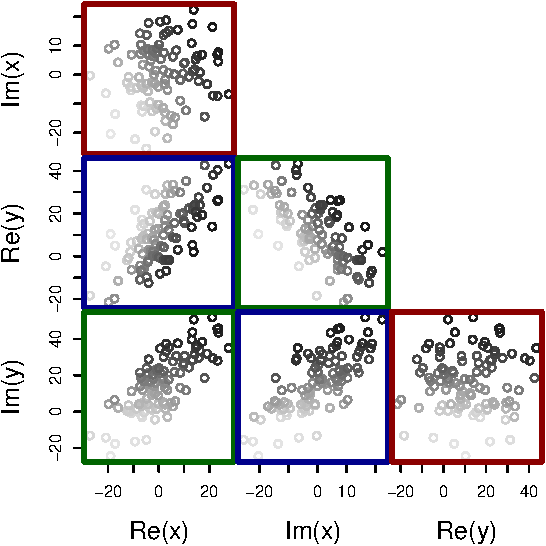
\includegraphics{Svetunkov---Svetunkov---Complex-Valued-Econometrics_files/figure-latex/crvCorConjugate-1.pdf}
\caption{\label{fig:crvCorConjugate}Two complex variables with conjugate correlation being close to one.}
\end{figure}

\begin{Shaded}
\begin{Highlighting}[]
\CommentTok{\# Conjugate correlation}
\KeywordTok{ccor}\NormalTok{(x, y, }\DataTypeTok{method=}\StringTok{"conjugate"}\NormalTok{)}
\end{Highlighting}
\end{Shaded}

\begin{verbatim}
## [1] 0.9975691
\end{verbatim}

As can be seen from the Figure \ref{fig:crvCorConjugate} and the value of the conjugate correlation, there is a relation between the two complex variables \(\underline{x}\) and \(\underline{y}\). The conjugate correlation says that this is a strong linear relation, and one of ways how we can check this is by analysing the MDS of the two variables.

\begin{Shaded}
\begin{Highlighting}[]
\KeywordTok{cplot}\NormalTok{(x, y, }\DataTypeTok{which=}\DecValTok{2}\NormalTok{, }\DataTypeTok{main=}\StringTok{""}\NormalTok{)}
\end{Highlighting}
\end{Shaded}

\begin{figure}
\centering
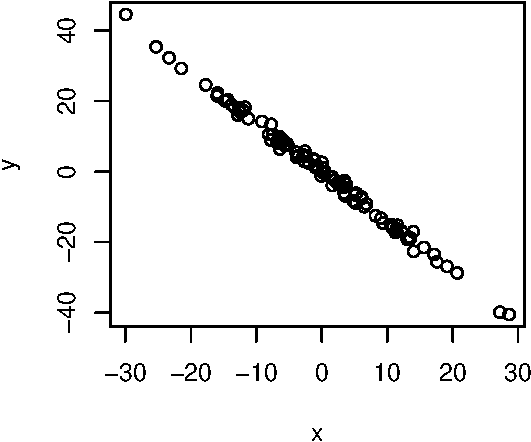
\includegraphics{Svetunkov---Svetunkov---Complex-Valued-Econometrics_files/figure-latex/crvCorConjugateMDS-1.pdf}
\caption{\label{fig:crvCorConjugateMDS}Visualisation of relations between two complex variables}
\end{figure}

As can be seen from the plot in Figure \ref{fig:crvCorConjugateMDS}, it seems that the variables indeed exhibit a strong linear relation. So, the conjugate correlation has provided an adequate information about it.

\hypertarget{correlationDirect}{%
\section{Direct correlation}\label{correlationDirect}}

The direct correlation can be expanded to:
\begin{equation}
    {\varrho}_{x,y} = \frac{\sigma_{x_r, y_r} - \sigma_{x_i, y_i} + i (\sigma_{x_i, y_r} + \sigma_{x_r, y_i})}{\sqrt{(\sigma_{x_r}^2 - \sigma_{x_i}^2 + i2 \sigma_{x_r,x_i})(\sigma_{y_r}^2 - \sigma_{y_i}^2 + i2 \sigma_{y_r,y_i})}}.
    \label{eq:correlationPseudoExpanded}
\end{equation}
Given that it contains a complex number in the denominator, it is more complicated than the conjugate one. But it has several apparent properties:

\begin{enumerate}
\def\labelenumi{\arabic{enumi}.}
\item
  The magnitude of the coefficient will be equal to zero (and thus the coefficient will be equal to zero) only when \(\sigma_{x_i,y_r}=\sigma_{x_r,y_i}=0\) and \(\sigma_{x_r,y_r}=\sigma_{x_i,y_i}\). One of the special cases of this is when all cross-covariances between the real and imaginary parts of \(\underline{x}\) and \(\underline{y}\) are equal to zero.
\item
  When the complex variables \(\underline{x}\) and \(\underline{y}\) have functional relation between them, so that \(\underline{a}_1 = \frac{1}{\underline{b}_1}\), the coefficient will be equal to one.
\end{enumerate}

Note however that due to the division by a complex number, the value of 1 can also be obtained due to the values of direct variance of variables \(\underline{x}\) and/or \(\underline{y}\).

Coefficient equal to -1 and to i.

\hypertarget{correlationMDSPearson}{%
\section{Pearson's correlation}\label{correlationMDSPearson}}

We can also use MDS to analyse the projections of complex variables on x and y axes, similar to how we have done that in Subsection \ref{correlationVisual}. In that case, we can calculate Pearson's correlation coefficient:

\begin{Shaded}
\begin{Highlighting}[]
\CommentTok{\# Create projections of two complex variables onto axes}
\KeywordTok{complex2vec}\NormalTok{(x) }\OperatorTok{|}\ErrorTok{\textgreater{}}\StringTok{ }\KeywordTok{dist}\NormalTok{() }\OperatorTok{|}\ErrorTok{\textgreater{}}\StringTok{ }\KeywordTok{cmdscale}\NormalTok{(}\DataTypeTok{k=}\DecValTok{1}\NormalTok{) {-}\textgreater{}}\StringTok{ }\NormalTok{xScaled}
\KeywordTok{complex2vec}\NormalTok{(y) }\OperatorTok{|}\ErrorTok{\textgreater{}}\StringTok{ }\KeywordTok{dist}\NormalTok{() }\OperatorTok{|}\ErrorTok{\textgreater{}}\StringTok{ }\KeywordTok{cmdscale}\NormalTok{(}\DataTypeTok{k=}\DecValTok{1}\NormalTok{) {-}\textgreater{}}\StringTok{ }\NormalTok{yScaled}
\CommentTok{\# Calculate the correlation coefficient}
\KeywordTok{cor}\NormalTok{(xScaled,yScaled)}
\end{Highlighting}
\end{Shaded}

\begin{verbatim}
##           [,1]
## [1,] -0.997186
\end{verbatim}

Or using the \texttt{ccor()} function with \texttt{method="pearson"}, which does exactly the same thing in one line of code:

\begin{Shaded}
\begin{Highlighting}[]
\KeywordTok{ccor}\NormalTok{(x, y, }\DataTypeTok{method=}\StringTok{"pearson"}\NormalTok{) }\OperatorTok{|}\ErrorTok{\textgreater{}}\StringTok{ }\KeywordTok{round}\NormalTok{(}\DecValTok{3}\NormalTok{)}
\end{Highlighting}
\end{Shaded}

The interpretation of the coefficient is straightforward and follows the conventional interpretation taught in any Statistics module. Note however that in general in the optimisation phase of MDS, it can reach the local optimum and not being able to get to the global one. As a result, the sign of the correlation might not represent the real relation between the two complex variables and in general should be ignored. Furthermore, inevitably when we move from four dimensions to two, we loose some information, so this approach is prone to possible mistakes and should be used with care. Finally, MDS is computationally expensive, especially on the long series. This means that in some cases it might take plenty of time before we get the Pearson's correlation value. Nonetheless, this is an additional way of analysing relations between complex variables.

\hypertarget{correlation-matrix}{%
\section{Correlation matrix}\label{correlation-matrix}}

Finally, as discussed in Subsection \ref{crvSecondMoment}, it is possible to calculate the covariance matrix between two c.r.v. Based on that matrix, we can calculate the correlation matrix, which will summarise all the relations between the real and imaginary parts of \(\underline{x}\) and \(\underline{y}\). This is done by dividing each element of the covariance matrix by geometric means of variances of the variables under consideration. In R, this can be done using \texttt{covar()} function from the \texttt{complex} package and \texttt{cov2cor()} function from the \texttt{stats} package:

\begin{Shaded}
\begin{Highlighting}[]
\KeywordTok{cbind}\NormalTok{(x,y) }\OperatorTok{|}\ErrorTok{\textgreater{}}\StringTok{ }\KeywordTok{covar}\NormalTok{() }\OperatorTok{|}\ErrorTok{\textgreater{}}\StringTok{ }\KeywordTok{cov2cor}\NormalTok{() }\OperatorTok{|}\ErrorTok{\textgreater{}}\StringTok{ }\KeywordTok{round}\NormalTok{(}\DecValTok{3}\NormalTok{)}
\end{Highlighting}
\end{Shaded}

\begin{verbatim}
##       x_r    x_i    y_r   y_i
## x_r 1.000  0.056  0.703 0.743
## x_i 0.056  1.000 -0.667 0.707
## y_r 0.703 -0.667  1.000 0.050
## y_i 0.743  0.707  0.050 1.000
\end{verbatim}

This matrix will not tell us how the variables \(\underline{x}\) and \(\underline{y}\) are related overall, but it will contain information about each of their individual elements.

\hypertarget{multipleCLR}{%
\chapter{Multiple Complex Linear Regression}\label{multipleCLR}}

We now move to the discussion of the multiple cLR, the model that captures relations between one complex random variable, \(y_r + i y_i\) and a set of explanatory complex random variables.

\hypertarget{model-formulation}{%
\section{Model formulation}\label{model-formulation}}

Similarly to how the multiple linear regression is formulated for real valued variables, the multiple complex linear regression can be written as:
\begin{equation}
    \underline{y}_j = \underline{\beta}_0 + \underline{\beta}_1 \underline{x}_{1,j} + \underline{\beta}_2 \underline{x}_{2,j} + \dots + \underline{\beta}_{k-1} \underline{x}_{k-1,j} + \underline{\epsilon}_j,
    \label{eq:MultipleCLRComplex}
\end{equation}
where \(k-1\) is the number of complex random variables. Similarly to how it was done with SCLR in \eqref{eq:SimpleCLRSystem}, we can expand the formula \eqref{eq:MultipleCLRComplex} as a system of two equations, taking that every parameter and every variable in \eqref{eq:MultipleCLRComplex} is complex:
\begin{equation}
    \begin{aligned}
        y_{r,j} = & \beta_{0,r} + \beta_{1,r} x_{1,r,j} - \beta_{1,i} x_{1,i,j} + \dots + \beta_{k-1,r} x_{k-1,r,j} - \beta_{k-1,i} x_{k-1,i,j} + \epsilon_{r,j} \\
        y_{i,j} = & \beta_{0,i} + \beta_{1,r} x_{1,i,j} + \beta_{1,i} x_{1,r,j} + \dots + \beta_{k-1,r} x_{k-1,i,j} + \beta_{k-1,i} x_{k-1,r,j} + \epsilon_{i,j} .
    \end{aligned}
    \label{eq:MultipleCLRSystem}
\end{equation}
As can be seen from \eqref{eq:MultipleCLRSystem}, the multiple cLR captures more complex dynamics than the conventional multiple linear regression. Both parts of the system use the same set of parameters and explanatory variables, but in different combinations, resulting in a versatile modelling framework.

This system can be represented in a more compact form, similarly to \eqref{eq:SimpleCLRVector}:
\begin{equation}
    \underline{\mathbf{y}} = \underline{\mathbf{X}} \underline{\boldsymbol{\beta}} + \underline{\boldsymbol{\epsilon}} ,
    \label{eq:CLRVector}
\end{equation}
where now \(\underline{\mathbf{X}} = \begin{pmatrix} 1 & \underline{x}_{1,1} & \dots & \underline{x}_{k-1,1} \\ 1 & \underline{x}_{1,2} & \dots & \underline{x}_{k-1,2} \\ \vdots & \vdots & \ddots & \vdots \\ 1 & \underline{x}_{1,n} & \dots & \underline{x}_{k-1,n} \end{pmatrix}\) and \(\underline{\boldsymbol{\beta}} = \begin{pmatrix} \underline{\beta}_0 \\ \underline{\beta}_1 \\ \vdots \\ \underline{\beta}_{k-1} \end{pmatrix}\), where each of the elements in the matrices and vectors above is a complex number.

Furthermore, the system \eqref{eq:MultipleCLRSystem} can also be used to represent the multiple cLR in a simple form using vector and matrix notations, avoiding complex numbers:
\begin{equation}
    \mathbf{y}_j = \underset{\sim}{\mathbf{X}_j} \boldsymbol{\beta} + \boldsymbol{\epsilon}_j ,
    \label{eq:MultipleCLRSystemVector}
\end{equation}
where \(\mathbf{y}_j = \begin{pmatrix} y_{r,j} \\ y_{i,j} \end{pmatrix}\), \(\underset{\sim}{\mathbf{X}_j} = \begin{pmatrix} 1 & 0 & x_{1,r,j} & -x_{1,i,j} & \dots & x_{k-1,r,j} & -x_{k-1,i,j} \\ 0 & 1 & x_{1,i,j} & x_{1,r,j} & \dots & x_{k-1,i,j} & x_{k-1,r,j} \end{pmatrix}\), \(\boldsymbol{\beta}^\prime = \begin{pmatrix} \beta_{0,r} & \beta_{0,i} & \beta_{1,r} & \beta_{1,i} & \dots & \beta_{1,k-1} & \beta_{1,k-1} \end{pmatrix}\) and \(\mathbf{\epsilon}_j = \begin{pmatrix} \epsilon_{r,j} \\ \epsilon_{i,j} \end{pmatrix}\). This can be then represented in the even more compact form, using the same principles as discussed in Section \ref{simpleCLRModel} in formula \eqref{eq:SimpleCLRSystemVectorFinal}:
\begin{equation}
    \mathbf{Y} = \underset{\sim}{\mathbf{X}} \boldsymbol{\beta} + \mathbf{E} 
    \label{eq:CLRSystemVectorFinal}
\end{equation}
where \(\mathbf{Y}=\begin{pmatrix}\mathbf{y}_1 \\ \mathbf{y}_2\\ \vdots \\ \mathbf{y}_n \end{pmatrix}\), \(\underset{\sim}{\mathbf{X}}=\begin{pmatrix} \underset{\sim}{\mathbf{X}_1} \\ \underset{\sim}{\mathbf{X}_2} \\ \vdots \\ \underset{\sim}{\mathbf{X}_n} \end{pmatrix}\) and \(\mathbf{E}=\begin{pmatrix}\boldsymbol{\epsilon}_1 \\ \boldsymbol{\epsilon}_2\\ \vdots \\ \boldsymbol{\epsilon}_n \end{pmatrix}\). Formula \eqref{eq:CLRSystemVectorFinal} becomes especially useful for multiple cLR for the model estimation via OLS, CLS or Likelihood in the matrix form. The form \eqref{eq:CLRSystemVectorFinal} sidesteps complex numbers all together, representing the set of equations in matrices and vectors, containing real numbers only. This is convenient for many purposes and in inference.

The main difference between the form \eqref{eq:CLRVector} and \eqref{eq:CLRSystemVectorFinal} is that the former contains complex numbers inside each of the matrices and vectors.

\hypertarget{mlcrEstimation}{%
\section{Estimation}\label{mlcrEstimation}}

In order to estimate the parameters of the model \eqref{eq:CLRVector}, we can use the same methods as in the Chapter \ref{simpleCLR}: OLS, CLS and Likelihood. We will write the estimated model as:
\begin{equation}
    \underline{\mathbf{y}} = \underline{\mathbf{X}} \underline{\boldsymbol{b}} + \underline{\mathbf{e}} ,
    \label{eq:CLRVectorEstimated}
\end{equation}
where \(\underline{\boldsymbol{b}}\) is the estimate of \(\underline{\boldsymbol{\beta}}\) and \(\underline{\mathbf{e}}\) is the estimate of \(\underline{\mathbf{\epsilon}}\). And in case of matrix notations, instead of \eqref{eq:CLRSystemVectorFinal} we will have:
\begin{equation}
    \mathbf{Y} = \underset{\sim}{\mathbf{X}} \boldsymbol{b} + \mathbf{\hat{E}} 
    \label{eq:CLRSystemVectorFinalEstimated}
\end{equation}

\hypertarget{ordinary-least-squares}{%
\subsection{Ordinary Least Squares}\label{ordinary-least-squares}}

The criterion of OLS for multiple cLR can be written as:
\begin{equation}
    \min S^{\mathrm{OLS}}(\underline{\boldsymbol{b}}) = \min \left(\underline{\mathbf{e}}^\prime \underline{\mathbf{e}}\right),
    \label{eq:CLROLSCriterion}
\end{equation}
which can be expanded to:
\begin{equation}
    \begin{aligned}
    S^{\mathrm{OLS}}(\underline{\boldsymbol{b}}) = & \left( \underline{\mathbf{y}} - \underline{\mathbf{X}} \underline{\boldsymbol{b}} \right)^\prime \left( \underline{\mathbf{y}} - \underline{\mathbf{X}} \underline{\boldsymbol{b}} \right) = \\
    & \underline{\mathbf{y}}^\prime \underline{\mathbf{y}} - \underline{\mathbf{y}}^\prime \underline{\mathbf{X}} \underline{\boldsymbol{b}} - \underline{\boldsymbol{b}}^\prime \underline{\mathbf{X}}^\prime \underline{\mathbf{y}} + \underline{\boldsymbol{b}}^\prime \underline{\mathbf{X}}^\prime \underline{\mathbf{X}} \underline{\boldsymbol{b}}
    \end{aligned}. 
    \label{eq:CLROLSCriterionExpanded}
\end{equation}
Taking derivative of \eqref{eq:CLROLSCriterionExpanded} with respect to \(\underline{\boldsymbol{b}}\) and equating it to zero, results in the following system of normal equations:
\begin{equation}
    \underline{\mathbf{X}}^\prime \underline{\mathbf{X}} \underline{\boldsymbol{b}} = \underline{\mathbf{X}}^\prime \underline{\mathbf{y}} ,
    \label{eq:CLROLSSystemOfNormalEquations}
\end{equation}
which gives the classical formula for the estimation of parameters of the model \eqref{eq:CLRSystemVectorFinal}:
\begin{equation}
    \underline{\boldsymbol{b}} = \left( \underline{\mathbf{X}}^\prime \underline{\mathbf{X}} \right)^{-1} \underline{\mathbf{X}}^\prime \underline{\mathbf{y}}
    \label{eq:MCLROLSEstimate}
\end{equation}
Given that \eqref{eq:MCLROLSEstimate} corresponds to the classical OLS, it will maintain all of its conventional properties, i.e.~its estimates being unbiased, efficient and consistent. Note that, as discussed Subsection \ref{complexVariable}, the operator \(\prime\) denotes conjugate transposition, which means that for the special case of simple cLR, the formula \eqref{eq:MCLROLSEstimate} will become \eqref{eq:SimpleCLROLSLossParametersMoments}.

Finally, using the same principles, we can show that the estimates of parameters can be obtained if we use the form \eqref{eq:CLRSystemVectorFinalEstimated} instead of the vectors of complex variables:
\begin{equation}
    \boldsymbol{b} = \left( \underset{\sim}{\mathbf{\tilde{X}}}^\prime \underset{\sim}{\mathbf{X}}\right)^{-1} \underset{\sim}{\mathbf{\tilde{X}}}^\prime {\mathbf{Y}} .
    \label{eq:MCLROLSEstimateComplex}
\end{equation}
The form \eqref{eq:MCLROLSEstimateComplex} becomes especially useful for futher inference.

\hypertarget{complex-least-squares}{%
\subsection{Complex Least Squares}\label{complex-least-squares}}

As discussed in Section \ref{SCLREstimation}, there is also an alternative approach to estimation of cLR, the Complex Least Squares. In order to get the estimates based on it, we need to apply the same principles as with OLS, but directly to the form \eqref{eq:CLRVector}, i.e.~minimise the criterion (which is the same as the one discussed in Subsection \ref{SCLREstimationCLS}):
\begin{equation}
    \min S^{\mathrm{CLS}}(\underline{\boldsymbol{b}}) = \min \left(\underline{\mathbf{e}}^\top \underline{\mathbf{e}}\right).
    \label{eq:CLRCLSCriterion}
\end{equation}
Using the same logic as with OLS, it can be shown that the minimisation of this criterion implies the solution of the following system of normal equations:
\begin{equation}
    \underline{\mathbf{X}}^\top \underline{\mathbf{X}} \underline{\boldsymbol{b}} = \underline{\mathbf{X}}^\top \underline{\mathbf{y}} ,
    \label{eq:CLRCLSSystemOfNormalEquations}
\end{equation}
which then results in the following formula for the CLS estimate of parameters:
\begin{equation}
    \underline{\boldsymbol{b}} = \left( \underline{\mathbf{X}}^\top \underline{\mathbf{X}}\right)^{-1} \underline{\mathbf{X}}^\top \underline{\mathbf{y}} .
    \label{eq:MCLRCLSEstimate}
\end{equation}
For the simple cLR, the formula \eqref{eq:MCLRCLSEstimate} becomes equivalent to \eqref{eq:SimpleCLRCLSLossParameters}. The main difference between \eqref{eq:MCLRCLSEstimate} and \eqref{eq:MCLROLSEstimateComplex}, as we can see, is that in the CLS, the transposition is done without the conjugation.

Finally, based on the form \eqref{eq:CLRSystemVectorFinalEstimated}, it can be shown that the same estimates (but in a form of real-valued vector) can be obtained via:
\begin{equation}
    \boldsymbol{b} = \left( \underset{\sim}{\mathbf{X}}^\top \underset{\sim}{\mathbf{X}}\right)^{-1} \underset{\sim}{\mathbf{{X}}}^\top {\mathbf{Y}} .
    \label{eq:MCLRCLSEstimateTranspose}
\end{equation}
The two formulae \eqref{eq:MCLRCLSEstimate} and \eqref{eq:MCLRCLSEstimateTranspose} result in exactly the same values of parameters, but will be useful for inference in the following sections.

\hypertarget{CLREstimationIssue}{%
\subsection{Issues with OLS and CLS}\label{CLREstimationIssue}}

Note that both OLS and CLS imply that the individual contributions of the real and imaginary parts of the error term are lost, and that the estimates of parameters are obtained for an overall variance of the complex error. In case of the OLS, this can be seen from the criterion \eqref{eq:CLROLSCriterion}, the minimisation of which is equivalent to the minimisation of the sum of variances:
\begin{equation}
    \min S^{\mathrm{OLS}}(\underline{\boldsymbol{b}}) = \min \left(\underline{\mathbf{e}}^\prime \underline{\mathbf{e}}\right) \iff \min \left(\hat{\sigma}_{e_r}^2 + \hat{\sigma}_{e_i}^2 \right),
    \label{eq:CLROLSCriterionVariance}
\end{equation}
where \(\hat{\sigma}_{e_r}^2\) and \(\hat{\sigma}_{e_i}^2\) are the variances of the real and imaginary parts of the error term respectively. The connection becomes apparent if we recall tha the main assumption of a regression model is that the expectation of the error term equals to zero. Because of that, the estimates of OLS lead to averaged out performance, ignoring the individual contribution of \(e_r\) and \(e_i\) and the covariance between the parts.

When it comes to CLS, the criterion \eqref{eq:CLRCLSCriterion} implies that:
\begin{equation}
    \min S^{\mathrm{CLS}}(\underline{\boldsymbol{b}}) = \min \left(\underline{\mathbf{e}}^\top \underline{\mathbf{e}}\right) \iff \min \left(\hat{\sigma}_{e_r}^2 - \hat{\sigma}_{e_i}^2 + 2i \hat{\sigma}_{e_r, e_i} \right),
    \label{eq:CLRCLSCriterionVariance}
\end{equation}
which now takes the covariance into account but ignores the sizes of the individual variances of the real and imaginary parts of the complex residuals.

In order to take the individual variances and the covariance into account, we need to use a different criterion and, as a result, a different estimator. One of such estimators is the Maximum Likelihood Estimator (MLE).

\hypertarget{likelihood}{%
\subsection{Likelihood}\label{likelihood}}

Similarly to how it was done in Subsection \ref{SCLREstimationLikelihood}, we can make an assumption about the distribution of the error term of the cLR. The conventional one is that it follows a normal distribution. If we formulate the model in the vector form \eqref{eq:MultipleCLRSystemVector} then after being estimated it becomes:
\begin{equation}
    \mathbf{y}_j = \underset{\sim}{\mathbf{X}_j} \boldsymbol{b} + \boldsymbol{e}_j .
    \label{eq:MultipleCLRSystemVectorEstimated}
\end{equation}
The concentrated log-likelihood for the complex regression model \eqref{eq:MultipleCLRSystemVectorEstimated} will be exactly the same as for the simple cLR:
\begin{equation*}
    \ell^*(\boldsymbol{\theta}, \hat{\boldsymbol{\Sigma}}_\epsilon | \mathbf{Y}) = -\frac{n}{2} \left( 2 \log(2 \pi e) + \log | \hat{\boldsymbol{\Sigma}}_\epsilon | \right) ,
\end{equation*}
where (as a reminder)
\begin{equation*}
    \hat{\boldsymbol{\Sigma}}_\epsilon = \frac{1}{n} \sum_{j=1}^{n} \boldsymbol{e}_j \boldsymbol{e}_j^\prime .
\end{equation*}
Maximising this likelihood, as discussed in Subsection \ref{SCLREstimationLikelihood}, implies minimising Generalised Variance and guarantees that the estimates of parameters are efficient and consistent.

However, \citet{Lutkepohl2005} shows for multivariate models that the maximum of the likelihood gives the same estimates of parameters as the OLS as long as the Multivariate Normal distribution with zero covariance is assumed for the error term. The results might differ for the other distributions or for the case, when the covariance in \(\hat{\boldsymbol{\Sigma}}_\epsilon\) is not zero.

\hypertarget{MCLRInference}{%
\section{Inference}\label{MCLRInference}}

It is possible to calculate the variance of estimates of parameters, using the same approach as used in the conventional OLS for the real-valued regression, substituting the formula for parameters with either \eqref{eq:MCLROLSEstimate} or \eqref{eq:MCLRCLSEstimate}. In fact, in case of c.r.v., it is possible to calculate both direct and conjugate covariance matrices of parameters. These variance can then be used in hypothesis testing or confidence interval construction. In order to do that, we need to replace the actual value \(\underline{\mathbf{y}}\) with \(\underline{\mathbf{X}} \underline{\boldsymbol{\beta}} + \underline{\boldsymbol{\epsilon}}\) in the OLS formula \eqref{eq:MCLROLSEstimate}:
\begin{equation}
    \begin{aligned}
    \underline{\boldsymbol{b}}^{\text{OLS}} =
        & \left( \underline{\mathbf{X}}^\prime \underline{\mathbf{X}} \right)^{-1} \underline{\mathbf{X}}^\prime \underline{\mathbf{y}} = \\
        & \left( \underline{\mathbf{X}}^\prime \underline{\mathbf{X}} \right)^{-1} \underline{\mathbf{X}}^\prime (\underline{\mathbf{X}} \underline{\boldsymbol{\beta}} + \underline{\boldsymbol{\epsilon}}) = \\
        & \left( \underline{\mathbf{X}}^\prime \underline{\mathbf{X}} \right)^{-1} \underline{\mathbf{X}}^\prime \underline{\mathbf{X}} \underline{\boldsymbol{\beta}} + \left( \underline{\mathbf{X}}^\prime \underline{\mathbf{X}} \right)^{-1} \underline{\mathbf{X}}^\prime \underline{\boldsymbol{\epsilon}} = \\
        & \underline{\boldsymbol{\beta}} + \left( \underline{\mathbf{X}}^\prime \underline{\mathbf{X}} \right)^{-1} \underline{\mathbf{X}}^\prime \underline{\boldsymbol{\epsilon}} .
    \end{aligned}
    \label{eq:MCLROLSExpansion}
\end{equation}
One thing that becomes apparent from this expansion is that the OLS estimates of parameters for a multiple complex linear regression will be unbiased as long as the expectation of the error term \(\underline{\boldsymbol{\epsilon}}\) is zero and it is not correlated with the explanatory variables. It is easy to show that the same holds for the CLS estimates as well based on the following expanded formula:
\begin{equation}
    \underline{\boldsymbol{b}}^{\text{CLS}} = \underline{\boldsymbol{\beta}} + \left( \underline{\mathbf{X}}^\top \underline{\mathbf{X}} \right)^{-1} \underline{\mathbf{X}}^\top \underline{\boldsymbol{\epsilon}} .
    \label{eq:MCLRCLSExpansion}
\end{equation}
This is a standard result from the real-valued regression analysis, but it is useful to know that it holds for the both estimation methods in complex-valued regression as well.

Based on \eqref{eq:MCLROLSExpansion}, we can calculate the conjugate variance to get conjugate covariance matrix of parameters:
\begin{equation}
    \mathrm{V}\left( \underline{\boldsymbol{b}}^{\text{OLS}} \right) = \mathrm{V}\left( \underline{\boldsymbol{\beta}} + \left( \underline{\mathbf{X}}^\prime \underline{\mathbf{X}} \right)^{-1} \underline{\mathbf{X}}^\prime \underline{\boldsymbol{\epsilon}} \right) .
    \label{eq:MCLROLSVariance01}
\end{equation}
In the formula \eqref{eq:MCLROLSVariance01}, the true estimates of parameters \(\underline{\boldsymbol{\beta}}\) will be independent of the explanatory variables and the error term, so the formula can be represented as a sum of variances. Furthermore, the true parameters do not have any uncertainty, i.e.~\(\mathrm{V}\left( \underline{\boldsymbol{\beta}} \right) = 0\), meaning that the formula \eqref{eq:MCLROLSVariance01} can be transformed into:
\begin{equation}
    \begin{aligned}
        \mathrm{V}\left( \underline{\boldsymbol{b}}^{\text{OLS}} \right) =
        & \mathrm{V}\left(\left( \underline{\mathbf{X}}^\prime \underline{\mathbf{X}} \right)^{-1} \underline{\mathbf{X}}^\prime \underline{\boldsymbol{\epsilon}} \right) = \\
        & \mathrm{E}\left( \left( \underline{\mathbf{X}}^\prime \underline{\mathbf{X}} \right)^{-1} \underline{\mathbf{X}}^\prime \underline{\boldsymbol{\epsilon}} \widetilde{ \left( \left( \underline{\mathbf{X}}^\prime \underline{\mathbf{X}} \right)^{-1} \underline{\mathbf{X}}^\prime \underline{\boldsymbol{\epsilon}}\right)} \right) .
    \end{aligned}
    \label{eq:MCLROLSVariance02}
\end{equation}
We switch from the variance to the expectation in \eqref{eq:MCLROLSVariance02}, dropping the expectation of the term in the brackets from the formula because it will be equal to zero as long as the explanatory variables and the error term are uncorrelated (one of the classical assumptions of a regression model). The tilde over the second term in \eqref{eq:MCLROLSVariance02} shows that this is the conjugate of the original complex variable. Recalling distributive properties of the conjugation \eqref{eq:complexNumberConjugateDistributive}, the same formula can be rewritten as:
\begin{equation}
    \begin{aligned}
        \mathrm{V}\left( \underline{\boldsymbol{b}}^{\text{OLS}} \right) =
        & \mathrm{E}\left( \left( \underline{\mathbf{X}}^\prime \underline{\mathbf{X}} \right)^{-1} \underline{\mathbf{X}}^\prime \underline{\boldsymbol{\epsilon}} \left( \underline{\mathbf{X}}^\top \tilde{\underline{\mathbf{X}}} \right)^{-1} \underline{\mathbf{X}}^\top \tilde{\underline{\boldsymbol{\epsilon}}} \right) ,
    \end{aligned}
    \label{eq:MCLROLSVariance03}
\end{equation}
which uses the property: \(\tilde{\underline{\mathbf{X}}}^\prime = \underline{\mathbf{X}}^\top\)
The expectation of the product in \eqref{eq:MCLROLSVariance03} can be rewritten as a product of expectations plus a covariance between the terms:
\begin{equation}
    \begin{aligned}
        \mathrm{V}\left( \underline{\boldsymbol{b}}^{\text{OLS}} \right) =
        & \mathrm{E}\left( \left( \underline{\mathbf{X}}^\prime \underline{\mathbf{X}} \right)^{-1} \underline{\mathbf{X}}^\prime \underline{\boldsymbol{\epsilon}} \right) \mathrm{E}\left( \left( {\underline{\mathbf{X}}}^\top \tilde{\underline{\mathbf{X}}} \right)^{-1} {\underline{\mathbf{X}}}^\top \tilde{\underline{\boldsymbol{\epsilon}}} \right) + \\
        & \mathrm{cov}\left(\left( \underline{\mathbf{X}}^\prime \underline{\mathbf{X}} \right)^{-1} \underline{\mathbf{X}}^\prime \underline{\boldsymbol{\epsilon}}, \left( {\underline{\mathbf{X}}}^\top \tilde{\underline{\mathbf{X}}} \right)^{-1} {\underline{\mathbf{X}}}^\top \tilde{\underline{\boldsymbol{\epsilon}}} \right) = \\
        & \left( \underline{\mathbf{X}}^\prime \underline{\mathbf{X}} \right)^{-1} \underline{\mathbf{X}}^\prime \tilde{\underline{\mathbf{X}}} \left( {\underline{\mathbf{X}}}^\top \tilde{\underline{\mathbf{X}}} \right)^{-1 \prime}  \mathrm{cov}\left( \underline{\boldsymbol{\epsilon}}, \tilde{\underline{\boldsymbol{\epsilon}}} \right) = \\
        & \left( \underline{\mathbf{X}}^\prime \underline{\mathbf{X}} \right)^{-1} \underline{\mathbf{X}}^\prime \tilde{\underline{\mathbf{X}}} \left( {\underline{\mathbf{X}}}^\top \tilde{\underline{\mathbf{X}}} \right)^{-1 \prime}  \sigma_{\underline{\epsilon}}^2 ,
    \end{aligned}
    \label{eq:MCLROLSConjVar}
\end{equation}
where the expectations of each term are equal to zero as long as the classical regression assumptions hold and \(\sigma_{\underline{\epsilon}}^2\) is the conjugate variance of the error term. Using the same logic, it can be shown that the direct variance of parameters can be calculated as:
\begin{equation}
    \begin{aligned}
        \mathcal{V}\left( \underline{\boldsymbol{b}}^{\text{OLS}} \right) =
        & \left( \underline{\mathbf{X}}^\prime \underline{\mathbf{X}} \right)^{-1} \varsigma_{\underline{\epsilon}}^2 .
    \end{aligned}
    \label{eq:MCLROLSDirVar}
\end{equation}
Finally, in a similar fashion, conjugate and direct covariance matrices of parameters can be calculated for the CLS:
\begin{equation}
    \begin{aligned}
        \mathrm{V}\left( \underline{\boldsymbol{b}}^{\text{CLS}} \right) =
        & \left( \underline{\mathbf{X}}^\top \underline{\mathbf{X}} \right)^{-1} \underline{\mathbf{X}}^\top \tilde{\underline{\mathbf{X}}} \left( {\underline{\mathbf{X}}}^\prime \tilde{\underline{\mathbf{X}}} \right)^{-1 \top}  \sigma_{\underline{\epsilon}}^2 .
    \end{aligned}
    \label{eq:MCLRCLSConjVar}
\end{equation}
and
\begin{equation}
    \begin{aligned}
        \mathcal{V}\left( \underline{\boldsymbol{b}}^{\text{CLS}} \right) =
        & \left( \underline{\mathbf{X}}^\top \underline{\mathbf{X}} \right)^{-1} \varsigma_{\underline{\epsilon}}^2 .
    \end{aligned}
    \label{eq:MCLRCLSDirVar}
\end{equation}
for the CLS. Having both direct and conjugate variances for OLS and CLS, we can calculate individual variances for each of the parameters and covariances between them to form a classical covariance matrix. The general formula for this would be:
\begin{equation*}
    \begin{aligned}
        & \mathrm{V}_{\boldsymbol{b}_r} = \frac{\mathcal{R}\left(\mathrm{V}\left( \underline{\boldsymbol{b}} \right) \right)+\mathcal{R}\left(\mathcal{V}\left( \underline{\boldsymbol{b}} \right) \right)}{2} \\
        & \mathrm{V}_{\boldsymbol{b}_i} = \frac{\mathcal{R}\left(\mathrm{V}\left( \underline{\boldsymbol{b}} \right) \right)-\mathcal{R}\left(\mathcal{V}\left( \underline{\boldsymbol{b}} \right) \right)}{2} \\
        & \mathrm{V}_{\boldsymbol{b}_{r,i}} = \frac{\mathcal{I}\left(\mathcal{V}\left( \underline{\boldsymbol{b}} \right)\right)}{2}
    \end{aligned},
\end{equation*}
where \(\mathrm{V}_{\boldsymbol{b}_r}\) is the part of the covariance matrix of real values of parameters, \(\mathrm{V}_{\boldsymbol{b}_i}\) is the part of the covariance matrix of imaginary values of parameters and \(\mathrm{V}_{\boldsymbol{b}_{r,i}}\) is the part of the covariance matrix between the real and imaginary parts of parameters. The final covariance matrix can be formed as:
\begin{equation}
    \hat{{\boldsymbol{\Sigma}}}_\beta =
    \begin{pmatrix}
        \mathrm{V}_{\boldsymbol{b}_r} & \mathrm{V}_{\boldsymbol{b}_{r,i}} \\
        \mathrm{V}_{\boldsymbol{b}_{r,i}} & \mathrm{V}_{\boldsymbol{b}_i}
    \end{pmatrix}.
    \label{eq:MCLRCLSVariance}
\end{equation}

Finally, in case of the likelihood estimation, the covariance matrix of parameters cannot be calculated analytically, but can be obtained numerically via the Hessian calculation. Given the formulation in this case, there is no need to do any additional transformations, the matrix will contain the variances and covariances of each individual parameter of the model.

\hypertarget{demonstration-in-r}{%
\subsection{Demonstration in R}\label{demonstration-in-r}}

In R, the estimation of the cLR can be done using the \texttt{clm()} function from the \texttt{complex} package. The specific estimation method can be selected using the \texttt{loss} parameter. For demonstration purposes, we will create an artificial data and see how the estimators work.

\begin{Shaded}
\begin{Highlighting}[]
\KeywordTok{set.seed}\NormalTok{(}\DecValTok{41}\NormalTok{)}
\CommentTok{\# Sample size}
\NormalTok{obs \textless{}{-}}\StringTok{ }\DecValTok{100}
\CommentTok{\# Generate parameters}
\NormalTok{b0 \textless{}{-}}\StringTok{ }\DecValTok{100} \OperatorTok{{-}}\StringTok{ }\NormalTok{150i}
\NormalTok{b1 \textless{}{-}}\StringTok{ }\FloatTok{2.5} \OperatorTok{+}\StringTok{ }\FloatTok{1.5}\NormalTok{i}
\NormalTok{b2 \textless{}{-}}\StringTok{ }\FloatTok{1.5} \OperatorTok{{-}}\StringTok{ }\FloatTok{0.75}\NormalTok{i}
\CommentTok{\# Create the explanatory variables}
\NormalTok{x1 \textless{}{-}}\StringTok{ }\KeywordTok{rcnorm}\NormalTok{(obs, }\DataTypeTok{mu=}\DecValTok{100}\OperatorTok{+}\NormalTok{150i, }\DataTypeTok{sigma2=}\DecValTok{200}\NormalTok{, }\DataTypeTok{varsigma2=}\DecValTok{100}\NormalTok{)}
\CommentTok{\# Create the explanatory variables}
\NormalTok{x2 \textless{}{-}}\StringTok{ }\KeywordTok{rcnorm}\NormalTok{(obs, }\DataTypeTok{mu=}\DecValTok{150}\OperatorTok{+}\NormalTok{100i, }\DataTypeTok{sigma2=}\DecValTok{200}\NormalTok{, }\DataTypeTok{varsigma2=}\DecValTok{150}\NormalTok{)}
\CommentTok{\# Generate error term from the complex normal distribution}
\NormalTok{e \textless{}{-}}\StringTok{ }\KeywordTok{rcnorm}\NormalTok{(obs, }\DataTypeTok{mu=}\DecValTok{0}\NormalTok{, }\DataTypeTok{sigma2=}\DecValTok{200}\NormalTok{, }\DataTypeTok{varsigma2=}\DecValTok{80}\OperatorTok{+}\NormalTok{150i)}
\CommentTok{\# Generate the response variable}
\NormalTok{y \textless{}{-}}\StringTok{ }\NormalTok{b0 }\OperatorTok{+}\StringTok{ }\NormalTok{b1 }\OperatorTok{*}\StringTok{ }\NormalTok{x1 }\OperatorTok{+}\StringTok{ }\NormalTok{b2 }\OperatorTok{*}\StringTok{ }\NormalTok{x2 }\OperatorTok{+}\StringTok{ }\NormalTok{e}
\CommentTok{\# Form a data frame with the variables}
\NormalTok{dataArtificial \textless{}{-}}\StringTok{ }\KeywordTok{data.frame}\NormalTok{(}\DataTypeTok{y=}\NormalTok{y, }\DataTypeTok{x1=}\NormalTok{x1, }\DataTypeTok{x2=}\NormalTok{x2)}
\end{Highlighting}
\end{Shaded}

The data generated using the code above will have the same variances of the real and imaginary parts of \texttt{x1} and the different ones for the \texttt{x2}. Furthermore, it will have residuals with correlated real and imaginary parts. We expect that in this situation the likelihood would be more appropriate than either OLS, or CLS.

We start by estimating the model using OLS:

\begin{Shaded}
\begin{Highlighting}[]
\KeywordTok{clm}\NormalTok{(y}\OperatorTok{\textasciitilde{}}\NormalTok{., dataArtificial, }\DataTypeTok{loss=}\StringTok{"OLS"}\NormalTok{) }\OperatorTok{|}\ErrorTok{\textgreater{}}
\StringTok{    }\KeywordTok{summary}\NormalTok{()}
\end{Highlighting}
\end{Shaded}

\begin{verbatim}
## Complex Linear Regression estimated via clm()
## Response variable: y
## Loss function used in estimation: OLS
## Coefficients:
##                Estimate Std. Error Lower 2.5% Upper 97.5%  
## (Intercept)_r  103.7956    16.7547    70.5421    137.0491 *
## (Intercept)_i -151.3386    12.1603  -175.4735   -127.2037 *
## x1_r             2.4161     0.0724     2.2724      2.5597 *
## x1_i             1.4877     0.0525     1.3834      1.5919 *
## x2_r             1.5625     0.0632     1.4371      1.6879 *
## x2_i            -0.6895     0.0459    -0.7805     -0.5985 *
## 
## Error covariance matrix:
##         e_r     e_i
## e_r 96.1432 52.0283
## e_i 52.0283 50.6449
## 
## Sample size: 100
## Number of estimated parameters: 3
## Number of degrees of freedom: 97
\end{verbatim}

As we see from the output above, the estimates of parameters are reasonable and close to the ones used in the data generation, while the 95\% confidence intervals include the true values of parameters. While it does not mean that this will always be the case universally, this demonstration shows how the OLS works and how the confidence intervals of parameters (based on the standard errors) can be obtained using the \texttt{clm()} function.

Keeping in mind that the MLE should give similar (if not the same) estimates of parameters, we should expect that the command below should produce a very similar output to the one above:

\begin{Shaded}
\begin{Highlighting}[]
\KeywordTok{clm}\NormalTok{(y}\OperatorTok{\textasciitilde{}}\NormalTok{., dataArtificial, }\DataTypeTok{loss=}\StringTok{"likelihood"}\NormalTok{) }\OperatorTok{|}\ErrorTok{\textgreater{}}
\StringTok{    }\KeywordTok{summary}\NormalTok{()}
\end{Highlighting}
\end{Shaded}

\begin{verbatim}
## Complex Linear Regression estimated via clm()
## Response variable: y
## Loss function used in estimation: likelihood
## Coefficients:
##                Estimate Std. Error Lower 2.5% Upper 97.5%  
## (Intercept)_r  103.7631    16.8860    70.2424    137.2838 *
## (Intercept)_i -151.3386    12.2552  -175.6666   -127.0107 *
## x1_r             2.4169     0.0729     2.2721      2.5616 *
## x1_i             1.4877     0.0529     1.3826      1.5927 *
## x2_r             1.5625     0.0637     1.4361      1.6889 *
## x2_i            -0.6895     0.0462    -0.7812     -0.5977 *
## 
## Error covariance matrix:
##         e_r     e_i
## e_r 97.6559 52.8591
## e_i 52.8591 51.4379
## 
## Sample size: 100
## Number of estimated parameters: 4.5
## Number of degrees of freedom: 95.5
## Information criteria:
##      AIC     AICc      BIC     BICc 
## 1338.345 1338.869 1350.069 1351.275
\end{verbatim}

While the estimates of parameters are not exactly the same, they are very similar. The difference arises from the estimation routine in the two methods: the OLS has analytical formulae for the estimates of parameters, while the likelihood has to rely on a numerical optimisation. Note that the error covariance matrix estimated using likelihood is slightly different than the one from OLS. One of the reasons for this is because the maximisation of the likelihood implies in addition to the minimisation of variances also the maximisation of the covariance between the real and imaginary parts of the complex residuals. Note however that the difference is not substantial, both methods produced very similar results.

The CLS, on the other hand, will give other estimates of parameters:

\begin{Shaded}
\begin{Highlighting}[]
\KeywordTok{clm}\NormalTok{(y}\OperatorTok{\textasciitilde{}}\NormalTok{., dataArtificial, }\DataTypeTok{loss=}\StringTok{"CLS"}\NormalTok{) }\OperatorTok{|}\ErrorTok{\textgreater{}}
\StringTok{    }\KeywordTok{summary}\NormalTok{()}
\end{Highlighting}
\end{Shaded}

\begin{verbatim}
## Complex Linear Regression estimated via clm()
## Response variable: y
## Loss function used in estimation: CLS
## Coefficients:
##                Estimate Std. Error Lower 2.5% Upper 97.5%  
## (Intercept)_r   74.8585    22.6298    29.9447    119.7723 *
## (Intercept)_i -131.4084    31.7400  -194.4036    -68.4132 *
## x1_r             2.3853     0.1567     2.0743      2.6964 *
## x1_i             1.2779     0.1384     1.0031      1.5527 *
## x2_r             1.5833     0.0823     1.4198      1.7467 *
## x2_i            -0.6633     0.0613    -0.7850     -0.5416 *
## 
## Error covariance matrix:
##          e_r     e_i
## e_r 102.1875 51.3523
## e_i  51.3523 53.2803
## 
## Sample size: 100
## Number of estimated parameters: 3
## Number of degrees of freedom: 97
\end{verbatim}

The estimates of parameters in the output above are less efficient than the ones from OLS/likelihood (as expected), but they are still not far from the true values of parameters. Notably, the CLS produced the lowest covariance between the real and imaginary parts of the complex residuals, which makes sense given how the CLS loss is formulated.

This demonstration shows how simple it is to estimate a cLR on data and how its outputs can be read. As one can see, the outputs do not differ substantially from the ones of the real values models.

\hypertarget{capturing-uncertainty-in-the-multiple-clr}{%
\section{Capturing uncertainty in the multiple cLR}\label{capturing-uncertainty-in-the-multiple-clr}}

Having both direct and conjugate variances for OLS and CLS, it is possible to do several things:

\begin{enumerate}
\def\labelenumi{\arabic{enumi}.}
\tightlist
\item
  Construct confidence intervals for parameters;
\item
  Construct a confidence ellipse for each complex parameter;
\item
  Test hypothesis about each of parameters (univariate distribution);
\item
  Test hypothesis for each complex parameter (considering joint distribution);
\item
  Produce confidence intervals for the conditional expectation from the model (fitted values and point forecasts);
\item
  Produce prediction intervals for the actual values.
\end{enumerate}

The elements (1) and (3) can be done assuming that the Central Limit Theorem works and thus the estimates of parameters follow Normal distribution. This can be done using Student's t-statistics as discussed in Section 6.4 and 8.1 of \citet{SvetunkovSBA}. The elements (2) and (4) rely on a different distribution and can be done using Hotelling's T\(^2\) statistics, discussed in Subsection \ref{Hotelling}. When it comes to elements (5) and (6), we need to impose some assumptions on the complex error term of the model \(\underline{\epsilon}_j\). The most popular assumption in statistics is that \(\underline{\epsilon}_j \sim \mathcal{N}(\boldsymbol{0}, \boldsymbol{\Sigma}_\epsilon)\), where \(\boldsymbol{0}\) is the two-dimensional vector of zeroes and \(\boldsymbol{\Sigma}_\epsilon\) is the square two-by-two covariance matrix. The estimate of this matrix is typically obtained via the formula:
\begin{equation*}
    \hat{\boldsymbol{\Sigma}}_\epsilon = \frac{1}{n-\frac{k}{2}} \sum_{j=1}^{n} \boldsymbol{e}_j \boldsymbol{e}_j^\prime ,
\end{equation*}
where \(k\) is the number of estimated parameters and \(n-\frac{k}{2}\) is the number of degrees of freedom per part of the model, division by which reduces the bias in the estimation of the covariance matrix. The division of \(k\) by 2 is required to reflect the fact that the complex response variable consists of two parts and the whole complex-valued equation can be represented in a form of a system of two equations, where the same parameters are used in both parts. To make this clearer, consider the following model:
\begin{equation*}
    y_{r,1} + i y_{i,1} = (a_{r,1} + i a_{i,1}) (x_{r,1} + i x_{i,1}) + \epsilon_{r,1} + i \epsilon_{i,1} .
\end{equation*}
It can be estimated on one observation and in that case will have zero degrees of freedom. Another way to look at this problem is to calculate the number of degrees of freedom per series, which in case of complex-valued model comes to two series resulting in the same \(n-\frac{k}{2}\).

To calculate prediction intervals, we need to calculate the variance of the conditional mean of a complex linear model. In case of complex variables, we need both direct and conjugate variances conditional on the values of the available explanatory variables to get the full information about the distribution:
\begin{equation}
    \begin{aligned}
    \mathrm{V}\left(\underline{y}_j | \underline{x}_{1,j}, \dots, \underline{x}_{k-1,j} \right) = & \mathrm{V}\left(\underline{b}_0 + \underline{b}_1 \underline{x}_{1,j} + \underline{b}_2 \underline{x}_{2,j} + \dots + \underline{b}_{k-1} \underline{x}_{k-1,j} + \underline{\epsilon}_j\right) \\
    & \sum_{i=0}^{k-1} \underline{x}_{i,j}\underline{\tilde{x}}_{i,j} \mathrm{V}\left(\underline{b}_i \right) + 2 \sum_{i\neq l} \underline{x}_{i,j}\underline{\tilde{x}}_{l,j} \mathrm{cov}\left(\underline{b}_i, \underline{b}_l \right) + \sigma_{\underline{\epsilon}}^2
    \end{aligned},
    \label{eq:MultipleCLRComplexVarianceDir}
\end{equation}
where \(\mathrm{cov}(\cdot)\) is the conjugate covariance between the variables and \(\underline{x}_{0,j}=1+i\). Similarly, we can calculate the direct conditional variance:
\begin{equation}
    \begin{aligned}
    \mathcal{V}\left(\underline{y}_j | \underline{x}_{1,j}, \dots, \underline{x}_{k-1,j} \right) = & \sum_{i=0}^{k-1} \underline{x}_{i,j}\underline{\tilde{x}}_{i,j} \mathcal{V}\left(\underline{b}_i \right) + 2 \sum_{i\neq l} \underline{x}_{i,j}\underline{\tilde{x}}_{l,j} {cov}\left(\underline{b}_i, \underline{b}_l \right) + \varsigma_{\underline{\epsilon}}^2
    \end{aligned},
    \label{eq:MultipleCLRComplexVarianceConj}
\end{equation}
where \({cov}(\cdot)\) is the direct covariance. The formulae \eqref{eq:MultipleCLRComplexVarianceDir} and \eqref{eq:MultipleCLRComplexVarianceDir} can then be used to calculate the conditional variances of real and imaginary parts of the response variable together with a conditional covariance between them. We can then either form a covariance matrix and produce a predictive ellipse using formulae discussed in Subsection \ref{MVNorm} or consider each of the parts independently and create prediction intervals (also discussed in Subsection \ref{MVNorm}). Arguably, the latter is easier to work with than the former.

Finally, to produce confidence intervals, we can use the formulae \eqref{eq:MultipleCLRComplexVarianceDir} and \eqref{eq:MultipleCLRComplexVarianceDir}, dropping the \(\mathrm{V}\left(\underline{\epsilon}_j\right)\) and \(\mathcal{V}\left(\underline{\epsilon}_j\right)\), which will then give us direct and conjugate conditional variances of the predicted value.

\hypertarget{demonstration-in-r-1}{%
\subsection{Demonstration in R}\label{demonstration-in-r-1}}

Building on the same example of artificial data from the previous section, we will see how predictions from the cLR can be made. To that extent, we will use the first 80 observations to estimate cLR using likelihood and then use the last 20 for prediction:

\begin{Shaded}
\begin{Highlighting}[]
\NormalTok{CLRArtificial \textless{}{-}}\StringTok{ }\KeywordTok{clm}\NormalTok{(y}\OperatorTok{\textasciitilde{}}\NormalTok{., dataArtificial,}
                     \DataTypeTok{loss=}\StringTok{"likelihood"}\NormalTok{, }\DataTypeTok{subset=}\KeywordTok{c}\NormalTok{(}\DecValTok{1}\OperatorTok{:}\DecValTok{80}\NormalTok{))}
\end{Highlighting}
\end{Shaded}

After estimating the model, we produce forecasts with a 95\% prediction interval (see Figure \ref{fig:CLRArtificialForecast}):

\begin{Shaded}
\begin{Highlighting}[]
\KeywordTok{par}\NormalTok{(}\DataTypeTok{mfcol=}\KeywordTok{c}\NormalTok{(}\DecValTok{2}\NormalTok{,}\DecValTok{1}\NormalTok{), }\DataTypeTok{mar=}\KeywordTok{c}\NormalTok{(}\DecValTok{2}\NormalTok{,}\DecValTok{2}\NormalTok{,}\DecValTok{3}\NormalTok{,}\DecValTok{1}\NormalTok{))}
\KeywordTok{predict}\NormalTok{(CLRArtificial, }\KeywordTok{tail}\NormalTok{(dataArtificial,}\DecValTok{20}\NormalTok{),}
        \DataTypeTok{interval=}\StringTok{"prediction"}\NormalTok{) }\OperatorTok{|}\ErrorTok{\textgreater{}}
\StringTok{    }\KeywordTok{plot}\NormalTok{()}
\end{Highlighting}
\end{Shaded}

\begin{figure}
\centering
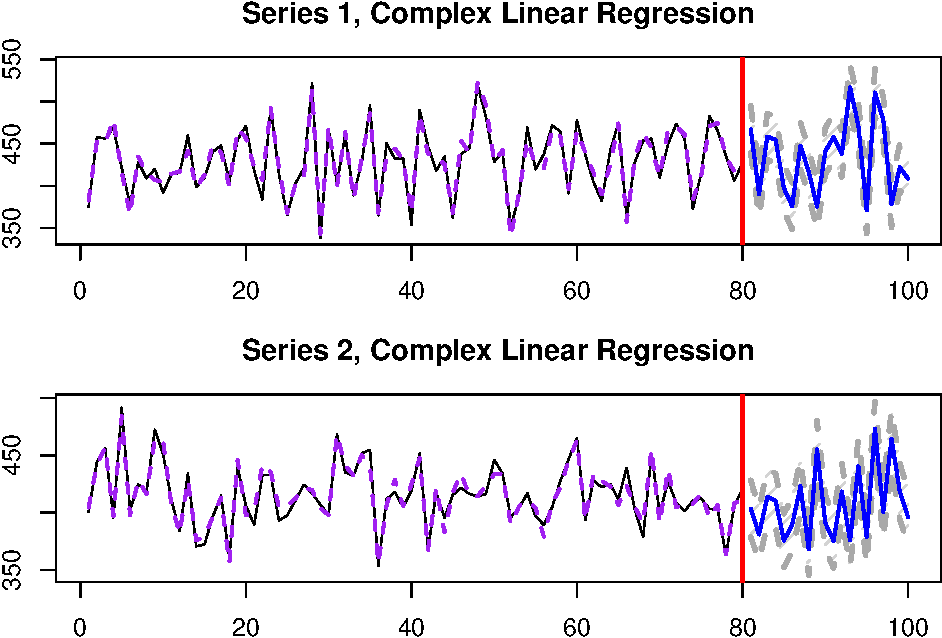
\includegraphics{Svetunkov---Svetunkov---Complex-Valued-Econometrics_files/figure-latex/CLRArtificialForecast-1.pdf}
\caption{\label{fig:CLRArtificialForecast}Forecasts from cLR for the artificial data, given the values of explanatory variables in the holdout set.}
\end{figure}

If the confidence interval for the conditional mean is needed, then this is regulated with \texttt{interval="confidence"} parameter.

\hypertarget{multipleCLRDummy}{%
\section{Dummy variables}\label{multipleCLRDummy}}

In the real-valued regression analysis, dummy variables appear when a feature of an object can be measured only in a categorical scale. For example, we might be interested in sales of a red medium size t-shirt vs the sales of a blue small size one. In this case, the colour would be one of such characteristics (measured in the nominal scale), while the size would be the other one (in ordinal scale). In order to include such information in the regression model, a set of dummy variables is typically created. A dummy variable is the variable that equals to one, when the feature exists and zero otherwise. So, in our example, we would create dummy variables \texttt{colourRed}, \texttt{colourBlue}, and \texttt{colourGreen} to denote the first feature and \texttt{sizeSmall}, \texttt{sizeMedium}, and \texttt{sizeLarge} for the second one. These variables would be equal to one for the specific observations (t-shirts) in our data. And for obvious reasons, the t-shirt cannot be both red and blue or small and medium at the same time, so the respective variables will be self-exclusive. If you want to learn more, you can find some information on that in Chapter 13 of \citet{SvetunkovSBA}.

In case of complex linear regression, it is possible to introduce dummy variables in the same way as in the conventional model, by adding real-valued variables. The model in this case becomes:

\begin{equation}
    \underline{y}_j = \underline{\beta}_0 + \underline{\beta}_1 \underline{x}_{1,j} + \dots + \underline{\beta}_{k-1} \underline{x}_{k-1,j} + \underline{\gamma}_1 d_{1,j} + \dots + \underline{\gamma}_m d_{m,j} + \underline{\epsilon}_j,
    \label{eq:MultipleCLRComplexDummy}
\end{equation}
where \(\underline{\gamma}_i\) is the complex parameter, \(d_{i,j}\) is th \(i\)-th real-valued dummy variable and \(m\) is the number of dummy variables. In this case, each variable \(d_{i,j}\) is multiplied by a complex coefficient, capturing the dummy effect of it on each part of the complex response variable. The effect of dummy variables on the response one is exactly the same as in the conventional real-valued regression - the intercept of the model, \(\underline{\beta}_0\) will change by the value of \(\underline{\gamma}_i\), when the variable \(d_{i,j}\) equals to one.

It is also theoretically possible to encode a complex dummy variable, which would have two features in it at the same time, e.g.~\(colourRed + i \times sizeSmall\), where both \texttt{colourRed} and \texttt{sizeSmall} are dummy variables. The issue with this is that this encoding assumes very specific dynamic between the features and the response variable. In the example above, the sales of the first product will have \(\gamma_{1,j} \times coolourRed_j - \gamma_{2,j} \times sizeSmall_j\), while the sales of the second one will have: \(\gamma_{1,j} \times sizeSmall_j + \gamma_{2,j} \times coolourRed_j\). This means that the red colour should have exactly the same impact on sales of product one, as the small size has on the product two, while the effect of small size on product one is opposite to the effect of the red colour on the second product. It is difficult to find situations, where such effects would be meaningful, so we do not recommend that. Still, it is possible to formulate such a model and capture the qualitative features in a parsimonious way (in comparison with a simple introduction of variables to each equation).

Finally, if an interaction effect is needed (e.g.~how the change of price on red product impacts its sales), this can be done in a similar way to the conventional real-valued regression. For example, here how it can be done for a variable \(\underline{x}_{1,j}\):
\begin{equation}
    \underline{y}_j = \underline{\beta}_0 + \underline{\beta}_1 \underline{x}_{1,j} + \dots + \underline{\beta}_{k-1} \underline{x}_{k-1,j} + \underline{\gamma}_1 \underline{x}_{1,j} d_{1,j} + \underline{\epsilon}_j .
    \label{eq:MultipleCLRComplexDummyInteraction}
\end{equation}
In this case, the specific complex effect of \(\underline{x}_{1,j}\) on \(\underline{y}_j\) will change when the dummy variable equals to one. The interaction effect between a complex variable \(\underline{x}_{1,j}\) and a complex dummy variable \(\underline{d}_{1,j}\) is also possible, but it will have a similar dilemma to the simple introduction of a dummy variable in a model.

\hypertarget{demonstration-in-r-2}{%
\subsection{Demonstration in R}\label{demonstration-in-r-2}}

The \texttt{clm()} function in the \texttt{complex} package in R supports categorical variables in a form of either a character vector, or a factor. Here is an example based on the same artificial data we used in Section \ref{MCLRInference}:

\begin{Shaded}
\begin{Highlighting}[]
\KeywordTok{set.seed}\NormalTok{(}\DecValTok{42}\NormalTok{)}
\CommentTok{\# Create an artificial categorical variable}
\NormalTok{x3 \textless{}{-}}\StringTok{ }\KeywordTok{rbinom}\NormalTok{(obs, }\DecValTok{2}\NormalTok{, }\FloatTok{0.5}\NormalTok{)}
\NormalTok{colour \textless{}{-}}\StringTok{ }\KeywordTok{vector}\NormalTok{(}\StringTok{"character"}\NormalTok{, obs)}
\NormalTok{colour[x3}\OperatorTok{==}\DecValTok{0}\NormalTok{] \textless{}{-}}\StringTok{ "Red"}\NormalTok{;}
\NormalTok{colour[x3}\OperatorTok{==}\DecValTok{1}\NormalTok{] \textless{}{-}}\StringTok{ "Green"}\NormalTok{;}
\NormalTok{colour[x3}\OperatorTok{==}\DecValTok{2}\NormalTok{] \textless{}{-}}\StringTok{ "Blue"}\NormalTok{;}
\CommentTok{\# Add it to the data frame}
\CommentTok{\# Note that it does not need to be factor()}
\NormalTok{dataArtificial \textless{}{-}}\StringTok{ }\KeywordTok{data.frame}\NormalTok{(}\DataTypeTok{y=}\NormalTok{y, }\DataTypeTok{x1=}\NormalTok{x1, }\DataTypeTok{x2=}\NormalTok{x2, }\DataTypeTok{colour=}\NormalTok{colour)}
\end{Highlighting}
\end{Shaded}

We can then estimate the model using the same command as before:

\begin{Shaded}
\begin{Highlighting}[]
\KeywordTok{clm}\NormalTok{(y}\OperatorTok{\textasciitilde{}}\NormalTok{x1}\OperatorTok{+}\NormalTok{x2}\OperatorTok{+}\NormalTok{colour, dataArtificial, }\DataTypeTok{loss=}\StringTok{"likelihood"}\NormalTok{) }\OperatorTok{|}\ErrorTok{\textgreater{}}
\StringTok{    }\KeywordTok{summary}\NormalTok{()}
\end{Highlighting}
\end{Shaded}

\begin{verbatim}
## Complex Linear Regression estimated via clm()
## Response variable: y
## Loss function used in estimation: likelihood
## Coefficients:
##                Estimate Std. Error Lower 2.5% Upper 97.5%  
## (Intercept)_r  103.5161    17.1840    69.3946    137.6377 *
## (Intercept)_i -157.3312    12.5342  -182.2198   -132.4425 *
## x1_r             2.4141     0.0729     2.2693      2.5590 *
## x1_i             1.4995     0.0532     1.3939      1.6052 *
## x2_r             1.5754     0.0643     1.4478      1.7030 *
## x2_i            -0.6765     0.0469    -0.7695     -0.5834 *
## colourGreen_r    3.2016     2.4187    -1.6012      8.0044  
## colourGreen_i    2.7011     1.7642    -0.8021      6.2043  
## colourRed_r     -0.1795     2.7961    -5.7317      5.3727  
## colourRed_i      1.9735     2.0395    -2.0763      6.0234  
## 
## Error covariance matrix:
##         e_r     e_i
## e_r 96.8123 52.4929
## e_i 52.4929 51.5081
## 
## Sample size: 100
## Number of estimated parameters: 6.5
## Number of degrees of freedom: 93.5
## Information criteria:
##      AIC     AICc      BIC     BICc 
## 1338.163 1339.217 1355.097 1357.524
\end{verbatim}

The output above shows that R expanded the colour into a set of dummy variables and dropped one of them (``blue''). The complex coefficients for the dummy variables are all not significant on the 5\% level, which in our case means that we cannot detect any strong relation between them and the response variable. This is because we did not use the variable in the data generation.

\hypertarget{example-of-application-of-complex-linear-regression}{%
\section{Example of Application of Complex Linear Regression}\label{example-of-application-of-complex-linear-regression}}

As a case study for the application of the cLR, we consider the macroeconomic data based on the Office for National Statistics (ONS) of the UK that has published information about several variables of interest:

\begin{enumerate}
\def\labelenumi{\arabic{enumi}.}
\tightlist
\item
  Capital - gross capital formation;
\item
  Labour - compensation of employees;
\item
  GDP - Gross Domestic Product;
\item
  NDP - Net Domestic Product;
\item
  DDP - Differences between GDP and NDP.
\end{enumerate}

We have collected the data for the period from 1990 to 2011 and our aim is to model is using cLR. To do that we use the principles discussed in Section \ref{complexModelling} and the production function model proposed by \citet{Svetunkov2014}, which can be written mathematically as:
\begin{equation}
    GDP + i DDP = (b_{0,r} + i b_{0,i}) \left(Capital + i Labour \right) ^{b_{1,r} + i b_{1,i}} \times (\epsilon_r + i \epsilon_i) .
    \label{eq:EnglandGDP}
\end{equation}

The data is available in the \texttt{complex} package in R under name \texttt{EnglandPF}. The data is shown in Figure \ref{fig:EnglandPF}.

\begin{Shaded}
\begin{Highlighting}[]
\KeywordTok{library}\NormalTok{(readxl, }\DataTypeTok{lib.loc =} \StringTok{"/usr/lib/R/library"}\NormalTok{)}
\NormalTok{EnglandPF \textless{}{-}}\StringTok{ }\KeywordTok{read\_excel}\NormalTok{(}\StringTok{"./data/England.xlsx"}\NormalTok{,}
                      \DataTypeTok{sheet=}\StringTok{"data"}\NormalTok{, }\DataTypeTok{range =} \StringTok{"A1:G23"}\NormalTok{)}
\NormalTok{EnglandPF \textless{}{-}}\StringTok{ }\NormalTok{EnglandPF[,}\OperatorTok{{-}}\DecValTok{2}\NormalTok{]}
\NormalTok{EnglandPF \textless{}{-}}\StringTok{ }\NormalTok{EnglandPF[,}\OperatorTok{{-}}\DecValTok{6}\NormalTok{]}
\KeywordTok{colnames}\NormalTok{(EnglandPF) \textless{}{-}}\StringTok{ }\KeywordTok{c}\NormalTok{(}\StringTok{"year"}\NormalTok{,}\StringTok{"Capital"}\NormalTok{,}\StringTok{"Labour"}\NormalTok{,}\StringTok{"GDP"}\NormalTok{,}\StringTok{"NDP"}\NormalTok{)}
\CommentTok{\# DDP {-} Difference of Domestic products}
\NormalTok{EnglandPF}\OperatorTok{$}\NormalTok{DDP \textless{}{-}}\StringTok{ }\NormalTok{EnglandPF}\OperatorTok{$}\NormalTok{GDP }\OperatorTok{{-}}\StringTok{ }\NormalTok{EnglandPF}\OperatorTok{$}\NormalTok{NDP}
\CommentTok{\# Make everything in millions pounds}
\NormalTok{EnglandPF[,}\OperatorTok{{-}}\DecValTok{1}\NormalTok{] \textless{}{-}}\StringTok{ }\NormalTok{EnglandPF[,}\OperatorTok{{-}}\DecValTok{1}\NormalTok{]}\OperatorTok{/}\FloatTok{1e+6}
\end{Highlighting}
\end{Shaded}

\begin{Shaded}
\begin{Highlighting}[]
\KeywordTok{plot}\NormalTok{(EnglandPF)}
\end{Highlighting}
\end{Shaded}

\begin{figure}
\centering
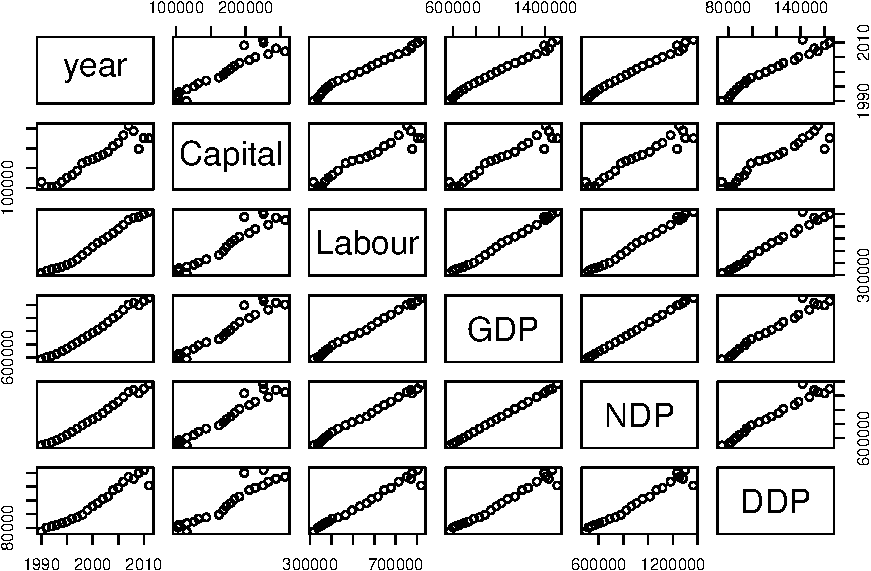
\includegraphics{Svetunkov---Svetunkov---Complex-Valued-Econometrics_files/figure-latex/EnglandPF-1.pdf}
\caption{\label{fig:EnglandPF}Dynamics of the macroeconomic variables from the ONS.}
\end{figure}

As we see, all variables exhibit strong trends (the first column of the plot) and thus have a strong linear relation between each other. To capture the trend in the data, we will introduce it explicitly as a real-valued variable in the model (this is discussed in Section \ref{DynamicTrend}), although taking differences is another possible solution (see Section \ref{DynamicARIMA}).

As discussed in Section \ref{complexModelling}, the variables need to be scaled in some way, we will use the standardisation:

\begin{Shaded}
\begin{Highlighting}[]
\CommentTok{\# Create a data frame of complex variables}
\NormalTok{EnglandComplex \textless{}{-}}
\StringTok{    }\KeywordTok{data.frame}\NormalTok{(}\DataTypeTok{y=}\KeywordTok{complex}\NormalTok{(}\DataTypeTok{real=}\NormalTok{EnglandPF}\OperatorTok{$}\NormalTok{GDP,}
                         \DataTypeTok{imaginary=}\NormalTok{EnglandPF}\OperatorTok{$}\NormalTok{DDP),}
               \DataTypeTok{x=}\KeywordTok{complex}\NormalTok{(}\DataTypeTok{real=}\NormalTok{EnglandPF}\OperatorTok{$}\NormalTok{Capital,}
                         \DataTypeTok{imaginary=}\NormalTok{EnglandPF}\OperatorTok{$}\NormalTok{Labour))}

\CommentTok{\# Standardise the complex variables}
\NormalTok{EnglandComplexScaled \textless{}{-}}
\StringTok{    }\KeywordTok{sapply}\NormalTok{(EnglandComplex, cscale, }\DataTypeTok{scaling=}\StringTok{"standardisation"}\NormalTok{)}
\end{Highlighting}
\end{Shaded}

Furthermore, in order to estimate the model \eqref{eq:EnglandGDP}, we will linearise it by taking logarithms of the both sides of the equation. All of this comes to the following R command:

\begin{Shaded}
\begin{Highlighting}[]
\NormalTok{EnglandcLR \textless{}{-}}\StringTok{ }\KeywordTok{clm}\NormalTok{(}\KeywordTok{log}\NormalTok{(y)}\OperatorTok{\textasciitilde{}}\KeywordTok{log}\NormalTok{(x)}\OperatorTok{+}\NormalTok{trend, EnglandComplexScaled)}
\end{Highlighting}
\end{Shaded}

The summary of the resulting model can be produced using the \texttt{summary()} command in R:

\begin{Shaded}
\begin{Highlighting}[]
\KeywordTok{summary}\NormalTok{(EnglandcLR)}
\end{Highlighting}
\end{Shaded}

\begin{verbatim}
## Complex Linear Regression estimated via clm()
## Response variable: logy
## Loss function used in estimation: likelihood
## Coefficients:
##               Estimate Std. Error Lower 2.5% Upper 97.5%  
## (Intercept)_r  -1.3377     0.3826    -2.1432     -0.5322 *
## (Intercept)_i   0.1196     0.3483    -0.6136      0.8529  
## log(x)_r        1.0723     0.0987     0.8645      1.2801 *
## log(x)_i        0.3812     0.0898     0.1921      0.5704 *
## trend_r         0.0876     0.0269     0.0310      0.1442 *
## trend_i        -0.0188     0.0245    -0.0703      0.0327  
## 
## Error covariance matrix:
##        e_r    e_i
## e_r 0.2334 0.1669
## e_i 0.1669 0.1934
## 
## Sample size: 22
## Number of estimated parameters: 4.5
## Number of degrees of freedom: 17.5
## Information criteria:
##     AIC    AICc     BIC    BICc 
## 34.4926 37.4926 39.4023 44.0388
\end{verbatim}

The output above can be interpreted based on what was discussed in Subsection \ref{complexVariable}: the coefficient \texttt{log(x)\_r} acts as the magnitude elasticity coefficient, showing that with the increase of the magnitude of the explanatory variable by 1\%, the resulting magnitude of the variable increases on average by 1.072\%. It also shows at the same time that the increase of the argument of the explanatory variable by 1 radiant leads to the increase of the response variable by 1.072 radians. In our case this means that with the increase of the proportion \(\frac{Labour}{Capital}\) the proportion \(\frac{DDP}{GDP}\) would tend to increase as well, i.e.~the decrease in the capital investments would imply the decrease in GDP and increase in DDP. This is enhanced by the parameter \texttt{log(x)\_i}, which increases the argument further, but at the same time decreasing the magnitude. Moreover, the parameter for the trend tells us that over time the magnitude tends to increase (both GDP and DDP increase), roughly by 8.8\% per year, while the argument of the response variable tends to decrease slowly, meaning that the GDP tends to increase faster than the DDP.

Finally, we can visualise the original data and the fitted model to see how the dynamics was captured, using the code below (Figure \ref{fig:EnglandPFFitted}):

\begin{Shaded}
\begin{Highlighting}[]
\CommentTok{\# Extract the fitted values and return them to the original scale}
\KeywordTok{fitted}\NormalTok{(EnglandcLR) }\OperatorTok{|}\ErrorTok{\textgreater{}}\StringTok{ }\KeywordTok{exp}\NormalTok{() }\OperatorTok{|}\ErrorTok{\textgreater{}}
\StringTok{    }\KeywordTok{cdescale}\NormalTok{(EnglandComplex}\OperatorTok{$}\NormalTok{y,}
             \DataTypeTok{scaling=}\StringTok{"standardisation"}\NormalTok{) {-}\textgreater{}}
\StringTok{    }\NormalTok{yFitted}

\CommentTok{\# Produce the plots}
\KeywordTok{par}\NormalTok{(}\DataTypeTok{mfcol=}\KeywordTok{c}\NormalTok{(}\DecValTok{2}\NormalTok{,}\DecValTok{1}\NormalTok{),}\DataTypeTok{mar=}\KeywordTok{c}\NormalTok{(}\DecValTok{4}\NormalTok{,}\DecValTok{4}\NormalTok{,}\DecValTok{1}\NormalTok{,}\DecValTok{1}\NormalTok{))}

\KeywordTok{plot}\NormalTok{(EnglandPF}\OperatorTok{$}\NormalTok{GDP,}\DataTypeTok{type=}\StringTok{"l"}\NormalTok{, }\DataTypeTok{ylab=}\StringTok{"GDP"}\NormalTok{, }\DataTypeTok{xlab=}\StringTok{"Time"}\NormalTok{)}
\KeywordTok{lines}\NormalTok{(}\KeywordTok{Re}\NormalTok{(yFitted), }\DataTypeTok{col=}\StringTok{"purple"}\NormalTok{, }\DataTypeTok{lwd=}\DecValTok{2}\NormalTok{, }\DataTypeTok{lty=}\DecValTok{2}\NormalTok{)}

\KeywordTok{plot}\NormalTok{(EnglandPF}\OperatorTok{$}\NormalTok{NDP,}\DataTypeTok{type=}\StringTok{"l"}\NormalTok{, }\DataTypeTok{ylab=}\StringTok{"NDP"}\NormalTok{, }\DataTypeTok{xlab=}\StringTok{"Time"}\NormalTok{)}
\KeywordTok{lines}\NormalTok{(}\KeywordTok{Re}\NormalTok{(yFitted)}\OperatorTok{{-}}\KeywordTok{Im}\NormalTok{(yFitted), }\DataTypeTok{col=}\StringTok{"purple"}\NormalTok{, }\DataTypeTok{lwd=}\DecValTok{2}\NormalTok{, }\DataTypeTok{lty=}\DecValTok{2}\NormalTok{)}
\end{Highlighting}
\end{Shaded}

\begin{figure}
\centering
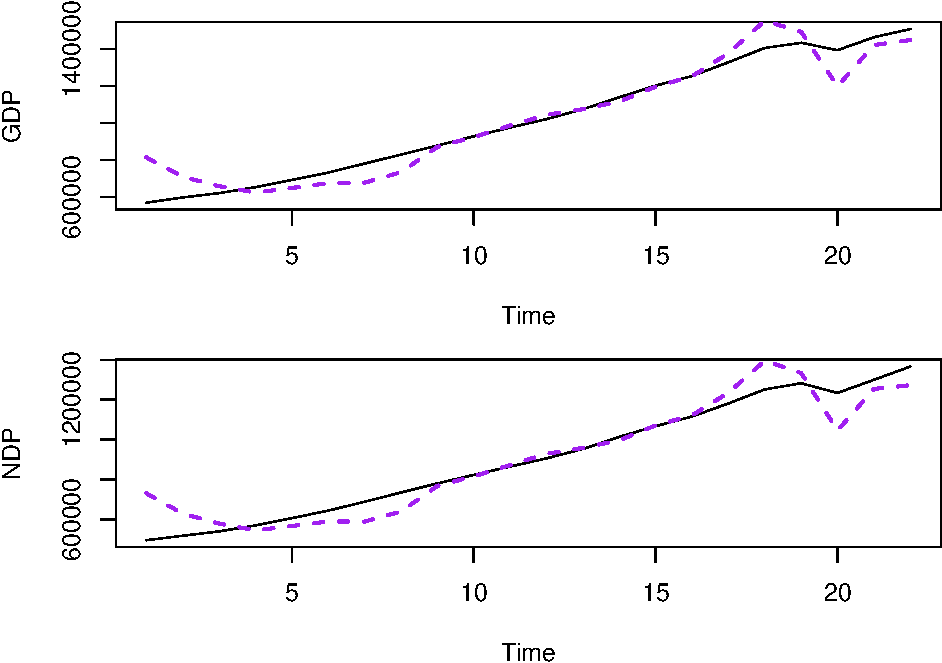
\includegraphics{Svetunkov---Svetunkov---Complex-Valued-Econometrics_files/figure-latex/EnglandPFFitted-1.pdf}
\caption{\label{fig:EnglandPFFitted}GDP and NDP with the fitted values from the cLR.}
\end{figure}

As we see, although the model fit is not perfect, it reflects the dynamics of GDP and NDP well with the fitted values following the actual values.

The estimated model can be used in the analysis of scenarios, e.g.~testing what will happen with GDP/NDP in case of the increase of the gross capital formation or the compensation of employees and for forecasting if the future values of the explanatory variables can be obtained or predicted.

\hypertarget{assumptions}{%
\chapter{Assumptions of Complex Linear Models}\label{assumptions}}

Similar to how it is done for the conventional real valued regression, we should discuss what assumptions are imposed on complex linear regression estimated using one of the methods discussed in the Section \ref{mlcrEstimation}. We will group all regression assumptions to three parts \citep[similar to how it was done by][]{SvetunkovAdam}:

\begin{enumerate}
\def\labelenumi{\arabic{enumi}.}
\tightlist
\item
  Model is correctly specified;
\item
  Residuals are independent and identically distributed (i.i.d.);
\item
  Explanatory variables are not correlated with anything but the response variable.
\end{enumerate}

While the first two groups directly relate to the so called ``true model'', the last one refers to the estimation approaches discussed in the previous Chapter: if the latter are violated then the estimation procedure will lead to issues in estimates of parameters. We should also point out that many of the assumptions discussed in this Chapter are very similar to the assumptions in the conventional regression, which is why we do not plan to cover them in this monograph in detail, but rather to focus on their implications to complex-valued models. An reader interested in assumptions for the real-valued models is advised to read Chapter 15 of \citet{SvetunkovSBA}.

\textbf{Disclaimer}: while in conventional econometrics, statistical tests are often used to check hypotheses of violation of specific assumptions, in this monograph we focus on the visual diagnostics. While tests might give ambiguous results and rely on a selected significance level, the visual inspection comes to expert judgment of an analyst. Yes, in some situations the subjectivity impacts the diagnostics, but at least it is not hidden behind p-values and a variety of outputs that might give contradictory results.

\hypertarget{assumptionsSpecification}{%
\section{Model is correctly specified}\label{assumptionsSpecification}}

This is one of the most general and most important groups of assumptions. It includes the following:

\begin{enumerate}
\def\labelenumi{\arabic{enumi}.}
\tightlist
\item
  Model does not omit any important variables;
\item
  Model does not have redundant variables;
\item
  Variables are included in the model with appropriate transformations;
\item
  Residuals of the model do not contain outliers.
\end{enumerate}

We briefly discuss all of them in this section.

\hypertarget{assumptionsSpecificationOmit}{%
\subsection{Model does not omit any important variables}\label{assumptionsSpecificationOmit}}

This assumption implies that we have all the variables that can substantially impact our response variable, and that we have included them in the model. If we do not do that then the estimates of parameters are known to be biased. In practice we always omit a lot of different variables that might potentially impact the response one, but do not have a large effect on it. Not including these variables is known not to cause serious issues in the estimation \citep{econometrics}.

Formally speaking, the omitted variables should not be correlated with the ones that we include in the model, because otherwise the impact of the latter will not be captured correctly, causing bias in the estimates of parameters. It is not possible to test this assumption, so it can only be checked based on judgment of an analyst.

When it comes to complex-valued models, the relations become much more complicated and potentially non-linear than in the conventional models. The problem becomes then manifolds: we need to include the correct variables in the model, but also they need to be included correctly, because now any variable can be included in the real or in the imaginary part. Furthermore, the correlation in complex-valued models can be measured differently and implies a variety of effects between two variables.

Practically speaking, we consider two situations with omitted variables:

\begin{enumerate}
\def\labelenumi{\arabic{enumi}.}
\tightlist
\item
  The model is estimated using OLS;
\item
  The model is estimated using CLS.
\end{enumerate}

For the both cases, we assume that the true model is of the form:
\begin{equation}
    \underline{\mathbf{y}} = \underline{\mathbf{X}} \underline{\boldsymbol{\beta}} + \underline{\mathbf{Z}} \underline{\boldsymbol{\gamma}} + \underline{\boldsymbol{\epsilon}},
    \label{eq:AssumptionsOmitTrueModel}
\end{equation}
where the matrix \(\underline{\mathbf{Z}}\) contains the variables omitted in the applied model and the vector \(\underline{\boldsymbol{\gamma}}\) is the vector of the parameters for these variables in the true model.

We start with the effect of the omitted variables on the estimates of parameters using OLS. We refer to the derivations \eqref{eq:MCLROLSExpansion}, which given \eqref{eq:AssumptionsOmitTrueModel} can be substituted to:
\begin{equation}
    \begin{aligned}
    \underline{\boldsymbol{b}}^{\text{OLS}} =
        & \left( \underline{\mathbf{X}}^\prime \underline{\mathbf{X}} \right)^{-1} \underline{\mathbf{X}}^\prime \underline{\mathbf{y}} = \\
        & \left( \underline{\mathbf{X}}^\prime \underline{\mathbf{X}} \right)^{-1} \underline{\mathbf{X}}^\prime \left(\underline{\mathbf{X}} \underline{\boldsymbol{\beta}} + \underline{\mathbf{Z}} \underline{\boldsymbol{\gamma}} + \underline{\boldsymbol{\epsilon}} \right) = \\
        & \left( \underline{\mathbf{X}}^\prime \underline{\mathbf{X}} \right)^{-1} \underline{\mathbf{X}}^\prime \underline{\mathbf{X}} \underline{\boldsymbol{\beta}} + \left( \underline{\mathbf{X}}^\prime \underline{\mathbf{X}} \right)^{-1} \underline{\mathbf{X}}^\prime \underline{\mathbf{Z}} \underline{\boldsymbol{\gamma}} + \left( \underline{\mathbf{X}}^\prime \underline{\mathbf{X}} \right)^{-1} \underline{\mathbf{X}}^\prime \underline{\boldsymbol{\epsilon}} = \\
        & \underline{\boldsymbol{\beta}} + \left( \underline{\mathbf{X}}^\prime \underline{\mathbf{X}} \right)^{-1} \underline{\mathbf{X}}^\prime \underline{\mathbf{Z}} \underline{\boldsymbol{\gamma}} + \left( \underline{\mathbf{X}}^\prime \underline{\mathbf{X}} \right)^{-1} \underline{\mathbf{X}}^\prime \underline{\boldsymbol{\epsilon}} .
    \end{aligned}
    \label{eq:AssumptionsOmitOLS01}
\end{equation}

Taking the expectation of \eqref{eq:AssumptionsOmitOLS01}, we get:
\begin{equation}
    \mathrm{E}\left(\underline{\boldsymbol{b}}^{\text{OLS}}\right) = \underline{\boldsymbol{\beta}} + \mathrm{E}\left(\left( \underline{\mathbf{X}}^\prime \underline{\mathbf{X}} \right)^{-1} \underline{\mathbf{X}}^\prime \underline{\mathbf{Z}} \underline{\boldsymbol{\gamma}} \right) + 0 ,
    \label{eq:AssumptionsOmitOLS02}
\end{equation}
with zero appearing because of the one of fundamental assumptions that the explanatory variables are not correlated with the error term in the true model. The expectation above shows that the estimates of the OLS parameters will be biased in case of omitted variables, and the bias will be proportional to the size of the \(\underline{\mathbf{X}}^\prime \underline{\mathbf{Z}}\) matrix, which consists of the covariances between the included and the omitted variables. The higher the correlation between these variables, the higher the bias will be. This agrees with the similar findings in the conventional real-valued econometrics.

When it comes to CLS, the logic is similar to the above. Based on the equations \eqref{eq:MCLRCLSExpansion} and \eqref{eq:AssumptionsOmitTrueModel} we have:
\begin{equation}
    \begin{aligned}
    \underline{\boldsymbol{b}}^{\text{CLS}} =
    & \left( \underline{\mathbf{X}}^\top \underline{\mathbf{X}}\right)^{-1} \underline{\mathbf{X}}^\top \underline{\mathbf{y}} = \\
    & \left( \underline{\mathbf{X}}^\top \underline{\mathbf{X}}\right)^{-1} \underline{\mathbf{X}}^\top \left(\underline{\mathbf{X}} \underline{\boldsymbol{\beta}} + \underline{\mathbf{Z}} \underline{\boldsymbol{\gamma}} + \underline{\boldsymbol{\epsilon}}\right) = \\
    & \underline{\boldsymbol{\beta}} + \left( \underline{\mathbf{X}}^\top \underline{\mathbf{X}}\right)^{-1} \underline{\mathbf{X}}^\top \underline{\mathbf{Z}} \underline{\boldsymbol{\gamma}} + \left( \underline{\mathbf{X}}^\top \underline{\mathbf{X}}\right)^{-1} \underline{\mathbf{X}}^\top \underline{\boldsymbol{\epsilon}}
    \end{aligned} ,
    \label{eq:AssumptionsOmitCLS01}
\end{equation}
which simplifies (using similar logic as above) to:
\begin{equation}
    \mathrm{E}\left(\underline{\boldsymbol{b}}^{\text{CLS}}\right) = \underline{\boldsymbol{\beta}} + \mathrm{E}\left( \left( \underline{\mathbf{X}}^\top \underline{\mathbf{X}}\right)^{-1} \underline{\mathbf{X}}^\top \underline{\mathbf{Z}} \underline{\boldsymbol{\gamma}}\right) ,
    \label{eq:AssumptionsOmitCLS02}
\end{equation}
Which also shows that the bias will increase with the increase of the values of the matrix \(\underline{\mathbf{X}}^\top \underline{\mathbf{Z}}\). The main difference between the real-valued and the complex-valued econometrics is that the aforementioned matrices are complex and the respective covariances in OLS and CLS are respectively conjugate and direct. This means that:

\begin{enumerate}
\def\labelenumi{\arabic{enumi}.}
\tightlist
\item
  if an omitted complex variable has high \emph{direct correlation} with the included one but has the zero \emph{conjugate correlation}, the OLS should give unbiased estimates of parameters, while the CLS would give the biased ones;
\item
  if an omitted complex variable has zero \emph{direct correlation} with the included one but has high \emph{conjugate correlation}, the CLS should give unbiased estimates of parameters, while the OLS would give the biased ones.
\end{enumerate}

This property can be used in deciding which of the estimation methods to use if the researcher has some insights about the relation between the included and the omitted complex variables.

Furthermore, we can also see what happens with the direct and conjugate covariance matrices of parameters in case of omitted variables. In the case of the omitted variables the residuals become \(\underline{\boldsymbol{\upsilon}} = \underline{\mathbf{Z}} \underline{\boldsymbol{\gamma}} + \underline{\boldsymbol{\epsilon}}\), implying that we estimate the following model instead of \eqref{eq:AssumptionsOmitTrueModel}:
\begin{equation}
    \underline{\mathbf{y}} = \underline{\mathbf{X}} \underline{\boldsymbol{\beta}} + \underline{\boldsymbol{\upsilon}} ,
    \label{eq:AssumptionsOmitAppliedTrueModel}
\end{equation}
which means that we then make inference based on:
\begin{equation}
    \underline{\mathbf{y}} = \underline{\mathbf{X}} \underline{\boldsymbol{b}} + \hat{\underline{\boldsymbol{\upsilon}}} .
    \label{eq:AssumptionsOmitAppliedModel}
\end{equation}

The covariance matrix of the estimates of the parameter \(\underline{\boldsymbol{\beta}}\) in this case comes to formulae discussed in Section \ref{MCLRInference}:
\begin{equation}
    \begin{aligned}
        & \mathrm{V}\left( \underline{\boldsymbol{b}}^{\text{OLS}} \right) = \left( \underline{\mathbf{X}}^\prime \underline{\mathbf{X}} \right)^{-1} \underline{\mathbf{X}}^\prime \tilde{\underline{\mathbf{X}}} \left( {\underline{\mathbf{X}}}^\top \tilde{\underline{\mathbf{X}}} \right)^{-1 \prime}  \sigma_{\underline{\upsilon}}^2 \\
        & \mathcal{V}\left( \underline{\boldsymbol{b}}^{\text{OLS}} \right) = \left( \underline{\mathbf{X}}^\prime \underline{\mathbf{X}} \right)^{-1} \varsigma_{\underline{\upsilon}}^2 \\
        & \mathrm{V}\left( \underline{\boldsymbol{b}}^{\text{CLS}} \right) = \left( \underline{\mathbf{X}}^\top \underline{\mathbf{X}} \right)^{-1} \underline{\mathbf{X}}^\top \tilde{\underline{\mathbf{X}}} \left( {\underline{\mathbf{X}}}^\prime \tilde{\underline{\mathbf{X}}} \right)^{-1 \top}  \sigma_{\underline{\upsilon}}^2 \\
        & \mathcal{V}\left( \underline{\boldsymbol{b}}^{\text{CLS}} \right) = \left( \underline{\mathbf{X}}^\top \underline{\mathbf{X}} \right)^{-1} \varsigma_{\underline{\upsilon}}^2 ,
    \end{aligned}
    \label{eq:MCLROLSCLSVariancesOmitted}
\end{equation}
where \(\sigma_{\underline{\upsilon}}^2\) is the conjugate and \(\varsigma_{\underline{\upsilon}}^2\) is the direct variances of the residuals \(\underline{\boldsymbol{\upsilon}}\). Now to better understand the effect of omitted variables on the covariance matrix of parameters, we should consider several situations:

\begin{enumerate}
\def\labelenumi{\arabic{enumi}.}
\tightlist
\item
  Some parts of \(\underline{\mathbf{Z}}\) are correlated with \(\underline{\mathbf{X}}\), in which case applying the model \eqref{eq:AssumptionsOmitAppliedModel} to the data will lead to the biased estimates of parameters, but would not have a large impact on the variance of the residuals of the model. The higher the correlation is, the lower the variances become in \eqref{eq:MCLROLSCLSVariancesOmitted};
\item
  \(\underline{\mathbf{Z}}\) is uncorrelated with \(\underline{\mathbf{X}}\), which means that the effect of the omitted variable is not captured by the model and as a result the variance of the residual \(\hat{\underline{\boldsymbol{\upsilon}}}\) will be inflated, increasing the standard errors of the estimates of parameters.
\end{enumerate}

The case (1) corresponds to the classical problem of the omitted variables in econometrics, while the case (2) shows how the uncertainty about the estimates of parameters increases with omitted variables and might lead to the wider confidence intervals for the parameters.

\hypertarget{assumptionsSpecificationRedundant}{%
\subsection{Model does not have redundant variables}\label{assumptionsSpecificationRedundant}}

This is the situation opposite to the first one. It implies that we have included something that should not be there. Mathematically it can be represented by two sets of equations, for the true and the applied models:
\begin{equation}
    \begin{aligned}
        & \underline{\mathbf{y}} = \underline{\mathbf{X}} \underline{\boldsymbol{\beta}} + \underline{\boldsymbol{\epsilon}} \\
        & \underline{\mathbf{y}} = \underline{\mathbf{X}} \underline{\boldsymbol{b}} + \underline{\mathbf{X}}_{red} \underline{\boldsymbol{b}}_{red} + \underline{\boldsymbol{e}} ,
    \end{aligned}
    \label{eq:AssumptionsRedundantSetting}
\end{equation}
where \(\underline{\boldsymbol{b}}_{red}\) is the vector of the estimates of parameters for the redundant variables \(\underline{\mathbf{X}}_{red}\) on a sample. It will not be zero in sample, because the values of \(\underline{\mathbf{X}}_{red}\) can explain some randomness in \(\underline{\mathbf{y}}\), thus reducing the size of variance of the residuals \(\underline{\boldsymbol{e}}\) in comparison with the estimation of the correct model. This leads to the effect known as ``overfitting'' in forecasting.

The second equation in \eqref{eq:AssumptionsRedundantSetting} can also be written in a compact form:
\begin{equation}
    \underline{\mathbf{y}} = \underline{\mathbf{Z}} \underline{\boldsymbol{c}}  + \underline{\boldsymbol{e}} ,
    \label{eq:AssumptionsRedundantAppliedModel}
\end{equation}
where \(\underline{\mathbf{Z}} = \begin{pmatrix} \underline{\mathbf{X}} & \underline{\mathbf{X}}_{red} \end{pmatrix}\) is the matrix that contains all variables under consideration, and \(\underline{\boldsymbol{c}} = \begin{pmatrix} \underline{\boldsymbol{b}} \\ \underline{\boldsymbol{b}}_{red} \end{pmatrix}\). While it is hard to show explicitly using formulae of OLS and CLS, it is well known in statistics that the estimates of parameters in such model are unbiased, because the true \(\underline{\boldsymbol{b}}_{red}\) is zero. At the same time, the inclusion of redundant variables increases the standard errors of parameters, because the covariance matrices from Section \ref{MCLRInference} would rely on different combinations of \(\underline{\mathbf{Z}}\) and its transposition (direct and conjugate), which means that the final variances would be impacted by the variability of redundant variables \(\underline{\mathbf{X}}_{red}\). The exact effect is difficult to capture and might depend on the direct/conjugate correlations between variables. We leave this task for future research.

\hypertarget{assumptionsSpecificationTransformation}{%
\subsection{Variables transformations}\label{assumptionsSpecificationTransformation}}

While the first two assumptions are universal for any statistical model, the third one has some special implications in case of cLR. This is because of the effect they have on the variables: transformations of separate parts of a complex variable are not equivalent to the transformations of the whole variable. For example, the logarithm of a complex variable \(\underline{z}\) as shown in \eqref{eq:complexNumberLogarithm} is:
\begin{equation*}
    \ln \underline{z} = \ln r + i \phi ,
\end{equation*}
which is not equivalent to the complex variable \(\ln x_r + i \ln x_i\). In fact, there is no known transformation from \(x_r + x_i\) to \(\ln x_r + i \ln x_i\) except for transforming separately the real and imaginary parts of the variable. Still, logarithms can be used to linearise a non-linear complex model to simplify its estimation. For example, the following multiplicative model (based on discussion in Subsection \ref{complexVariable}):
\begin{equation*}
    \begin{aligned}
    y_{r} + i y_{i} = & (\beta_{0,r} + i \beta_{0,i}) \times (x_{1,r} + i x_{1,i}) ^{\beta_{1,r} + i \beta_{1,i}} \times \dots \times \\
                      & (x_{k-1,r} + i x_{k-1,i}) ^{\beta_{k-1,r} + i \beta_{k-1,i}} \times (\epsilon_{r} + i \epsilon_{i})
    \end{aligned}
\end{equation*}
can be linearised using natural logarithm to:
\begin{equation*}
    \begin{aligned}
    \ln (y_{r} + i y_{i}) = & \ln (\beta_{0,r} + i \beta_{0,i}) + (\beta_{1,r} + i \beta_{1,i}) \ln(x_{1,r} + i x_{1,i}) + \dots + \\
                            & (\beta_{k-1,r} + i \beta_{k-1,i}) \ln (x_{k-1,r} + i x_{k-1,i}) + \ln (\epsilon_{r} + i \epsilon_{i}),
    \end{aligned}
\end{equation*}
which can then be estimated using OLS, CLS or likelihood maximisation as discussed in Section \ref{mlcrEstimation}. On its own, the multiplicative models of complex variables have useful features, because they allow modelling highly non-linear processes due to the rotation as discussed in Section \ref{theoryOfComplexNumbers}. For example, here how the linear increase of real and imaginary parts of a complex variable \(\underline{x}\) leads to a non-linear transform of a variable \(\underline{y}=\underline{x}^{0.5+0.5i}\):

\begin{Shaded}
\begin{Highlighting}[]
\NormalTok{x \textless{}{-}}\StringTok{ }\DecValTok{1}\OperatorTok{:}\DecValTok{100} \OperatorTok{+}\StringTok{ }\DecValTok{1}\OperatorTok{:}\DecValTok{100}\OperatorTok{*}\NormalTok{1i}
\NormalTok{y \textless{}{-}}\StringTok{ }\NormalTok{x}\OperatorTok{\^{}}\NormalTok{(}\FloatTok{0.5+0.5}\NormalTok{i)}
\KeywordTok{cplot}\NormalTok{(x, y)}
\end{Highlighting}
\end{Shaded}

\begin{figure}
\centering
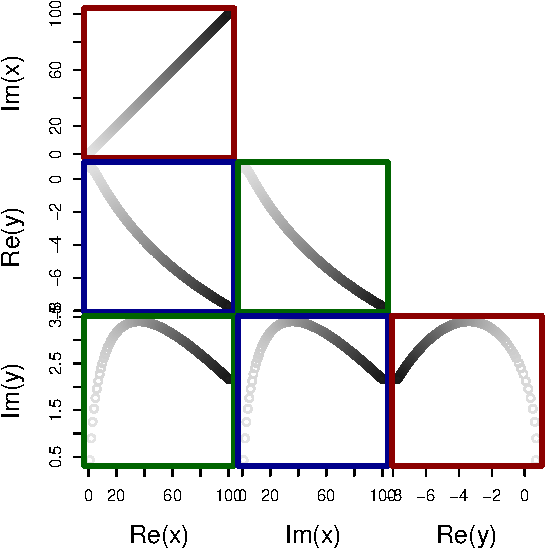
\includegraphics{Svetunkov---Svetunkov---Complex-Valued-Econometrics_files/figure-latex/unnamed-chunk-37-1.pdf}
\caption{\label{fig:unnamed-chunk-37}Non-linear transformation of a complex variable that changes linearly.}
\end{figure}

Even if the imaginary part of \(\underline{x}\) is zero (and as a result we deal with a real number, not a complex one), the complex power leads to highly non-linear transformation of the variable. This is a useful feature if the non-linearity is suspected in the data.

The diagnostics of correct transformations in cLR is challenging, but can be done by analysing the residuals. Consider the following example in R (using functions from the \texttt{complex} package in R):

\begin{Shaded}
\begin{Highlighting}[]
\CommentTok{\# Set random seed for reproducibility}
\KeywordTok{set.seed}\NormalTok{(}\DecValTok{41}\NormalTok{)}
\CommentTok{\# Sample size}
\NormalTok{obs \textless{}{-}}\StringTok{ }\DecValTok{1000}
\CommentTok{\# Create the explanatory variable}
\NormalTok{x \textless{}{-}}\StringTok{ }\KeywordTok{complex}\NormalTok{(}\DataTypeTok{real=}\KeywordTok{rnorm}\NormalTok{(obs,}\DecValTok{100}\NormalTok{,}\DecValTok{10}\NormalTok{), }\DataTypeTok{imaginary=}\KeywordTok{rnorm}\NormalTok{(obs,}\DecValTok{50}\NormalTok{,}\DecValTok{5}\NormalTok{))}
\CommentTok{\# Generate parameters}
\NormalTok{b0 \textless{}{-}}\StringTok{ }\DecValTok{1} \OperatorTok{{-}}\StringTok{ }\FloatTok{1.5}\NormalTok{i}
\NormalTok{b1 \textless{}{-}}\StringTok{ }\FloatTok{2.5} \OperatorTok{+}\StringTok{ }\FloatTok{1.5}\NormalTok{i}
\CommentTok{\# Generate error term from the complex normal distribution}
\NormalTok{e \textless{}{-}}\StringTok{ }\KeywordTok{rcnorm}\NormalTok{(obs, }\DecValTok{0}\NormalTok{, }\DataTypeTok{sigma2=}\FloatTok{0.25}\NormalTok{, }\DataTypeTok{varsigma2=}\FloatTok{0.16+0.09}\NormalTok{i)}
\CommentTok{\# Generate the data using non{-}linear model}
\NormalTok{y \textless{}{-}}\StringTok{ }\KeywordTok{exp}\NormalTok{(b0 }\OperatorTok{+}\StringTok{ }\NormalTok{b1 }\OperatorTok{*}\StringTok{ }\KeywordTok{log}\NormalTok{(x) }\OperatorTok{+}\StringTok{ }\NormalTok{e)}
\CommentTok{\# Merge it to the matrix}
\NormalTok{complexData \textless{}{-}}\StringTok{ }\KeywordTok{data.frame}\NormalTok{(}\DataTypeTok{y=}\NormalTok{y,}\DataTypeTok{x=}\NormalTok{x)}
\end{Highlighting}
\end{Shaded}

For demonstration purposes, we will first use a complex linear regression model on the data that was generated using a non-linear one:

\begin{Shaded}
\begin{Highlighting}[]
\CommentTok{\# Apply a linear model}
\NormalTok{complexModel \textless{}{-}}\StringTok{ }\KeywordTok{clm}\NormalTok{(y}\OperatorTok{\textasciitilde{}}\NormalTok{x, complexData)}
\end{Highlighting}
\end{Shaded}

The issues of the model can be diagnosed using various plots. For example, here how the standardised residuals vs fitted would look for the model above (see Figure \ref{fig:nonlinearLinStdResid}):

\begin{Shaded}
\begin{Highlighting}[]
\KeywordTok{par}\NormalTok{(}\DataTypeTok{mfcol=}\KeywordTok{c}\NormalTok{(}\DecValTok{1}\NormalTok{,}\DecValTok{2}\NormalTok{), }\DataTypeTok{mar=}\KeywordTok{c}\NormalTok{(}\DecValTok{2}\NormalTok{,}\DecValTok{2}\NormalTok{,}\DecValTok{3}\NormalTok{,}\DecValTok{1}\NormalTok{))}
\KeywordTok{plot}\NormalTok{(complexModel, }\DataTypeTok{which=}\DecValTok{2}\NormalTok{, }\DataTypeTok{main=}\StringTok{""}\NormalTok{)}
\end{Highlighting}
\end{Shaded}

\begin{figure}
\centering
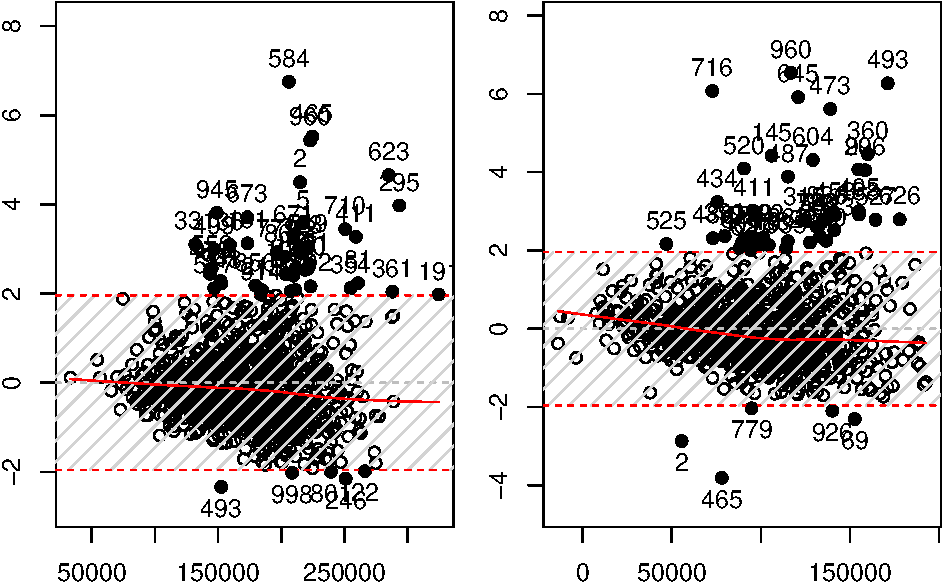
\includegraphics{Svetunkov---Svetunkov---Complex-Valued-Econometrics_files/figure-latex/nonlinearLinStdResid-1.pdf}
\caption{\label{fig:nonlinearLinStdResid}Standardised residuals vs Fitted for the cLR on non-linear data.}
\end{figure}

The plots above demonstrate that there is a slight non-linear pattern in the residuals (especially for the real part of the model) and that their variances might not be constant. These are the indicators of a possible non-linearity in the data. In order to capture it correctly, we would need to transform both response and the explanatory complex variables and estimate the model in logarithms:

\begin{Shaded}
\begin{Highlighting}[]
\CommentTok{\# Apply a model to log data}
\NormalTok{complexModelLogs \textless{}{-}}\StringTok{ }\KeywordTok{clm}\NormalTok{(}\KeywordTok{log}\NormalTok{(y)}\OperatorTok{\textasciitilde{}}\KeywordTok{log}\NormalTok{(x), complexData)}
\end{Highlighting}
\end{Shaded}

After which the same plot will look more reasonable, with residuals not exhibiting a strong u-shape anymore (see Figure \ref{fig:nonlinearStdResid}):

\begin{Shaded}
\begin{Highlighting}[]
\KeywordTok{par}\NormalTok{(}\DataTypeTok{mfcol=}\KeywordTok{c}\NormalTok{(}\DecValTok{1}\NormalTok{,}\DecValTok{2}\NormalTok{), }\DataTypeTok{mar=}\KeywordTok{c}\NormalTok{(}\DecValTok{2}\NormalTok{,}\DecValTok{2}\NormalTok{,}\DecValTok{3}\NormalTok{,}\DecValTok{1}\NormalTok{))}
\KeywordTok{plot}\NormalTok{(complexModelLogs, }\DataTypeTok{which=}\DecValTok{2}\NormalTok{, }\DataTypeTok{main=}\StringTok{""}\NormalTok{)}
\end{Highlighting}
\end{Shaded}

\begin{figure}
\centering
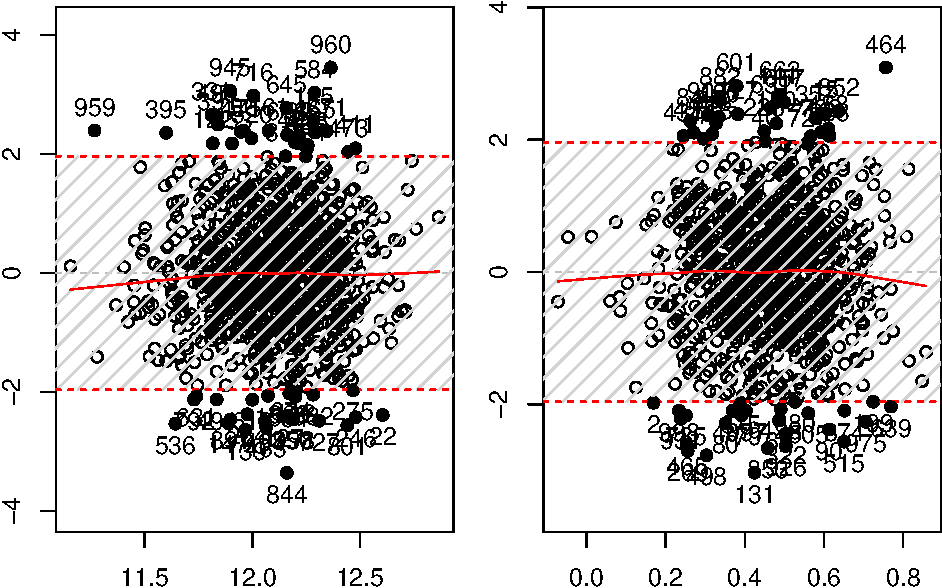
\includegraphics{Svetunkov---Svetunkov---Complex-Valued-Econometrics_files/figure-latex/nonlinearStdResid-1.pdf}
\caption{\label{fig:nonlinearStdResid}Standardised residuals vs Fitted for the log-log cLR on non-linear data.}
\end{figure}

\hypertarget{assumptionsSpecificationOutlier}{%
\subsection{No outliers}\label{assumptionsSpecificationOutlier}}

Finally, the presence of outliers in the residuals typically implies that either there is an error in recording the data, or the model omits an important variable (e.g.~a dummy variable for an external event). In that case the effect on estimates of parameters will be similar to the one discussed in Subsection \ref{assumptionsSpecificationOmit}: the estimates of parameters will be in general biased with some specific effects depending on the direct/conjugate correlation and the estimation method used.

The simplest way to detect outliers is to produce a diagnostic plot of fitted vs standardised residuals (similar to the one in Figure \ref{fig:nonlinearStdResid}) and analyse those values that lie outside of the constructed confidence interval. If the value of an outlier cannot be explained (e.g.~this is not a calendar event, this is not a promotion etc) then it can be removed or interpolated. In the latter case, creating a dummy variable (see Section \ref{multipleCLRDummy}) that equals to one on that specific observation and to zero on all the others is one of the simplest way of dealing with the outlier.

\hypertarget{assumptionsResiduals}{%
\section{Residuals are i.i.d.}\label{assumptionsResiduals}}

The next group of assumptions has five elements in it:

\begin{enumerate}
\def\labelenumi{\arabic{enumi}.}
\tightlist
\item
  Residuals are homoscedastic;
\item
  No autocorrelation in residuals;
\item
  Expectation of residuals is zero (no matter what);
\item
  Residuals follow an assumed distribution;
\item
  Residuals follow a circular distribution.
\end{enumerate}

Some of these assumptions are universal for statistical models, while the others (e.g.~the last one) are specific to cLR.

\hypertarget{assumptionsResidualsHomoscedastic}{%
\subsection{Homoscedastic residuals}\label{assumptionsResidualsHomoscedastic}}

The first assumption implies that both direct and conjugate variances of the residuals are constant and do not change with any changes of variables. This follows directly from the formulae for the direct and conjugate covariances from Section \ref{MCLRInference}: if either of the covariances is not constant, and we use the formulae for calculating the standard errors of parameters, we will obtain averaged-out values, that would be lower than needed for some observations and higher than needed for the others.

In case of the formulation of cLR as a vector model and the likelihood estimation, the assumption implies that the covariance matrix of residuals \(\Sigma_\epsilon\) stays the same no matter what. This assumption aligns well with a similar assumption of conventional multivariate models, such as VAR \citep{Lutkepohl} or VETS \citep{SvetunkovVETS}.

The homoscedasticity assumption can be typically diagnosed visually by producing the plot of absolute residuals vs fitted. In case of the cLR, this can be modified to producing plots for each part of the complex residuals. Figure \ref{fig:heteroDiagnostics} shows how the residuals of the linear model applied to the non-linear data (example from Subsection \ref{assumptionsSpecificationTransformation}) look:

\begin{Shaded}
\begin{Highlighting}[]
\KeywordTok{par}\NormalTok{(}\DataTypeTok{mfcol=}\KeywordTok{c}\NormalTok{(}\DecValTok{1}\NormalTok{,}\DecValTok{2}\NormalTok{), }\DataTypeTok{mar=}\KeywordTok{c}\NormalTok{(}\DecValTok{2}\NormalTok{,}\DecValTok{2}\NormalTok{,}\DecValTok{3}\NormalTok{,}\DecValTok{1}\NormalTok{))}
\KeywordTok{plot}\NormalTok{(complexModel, }\DataTypeTok{which=}\DecValTok{4}\NormalTok{, }\DataTypeTok{main=}\StringTok{""}\NormalTok{)}
\end{Highlighting}
\end{Shaded}

\begin{figure}
\centering
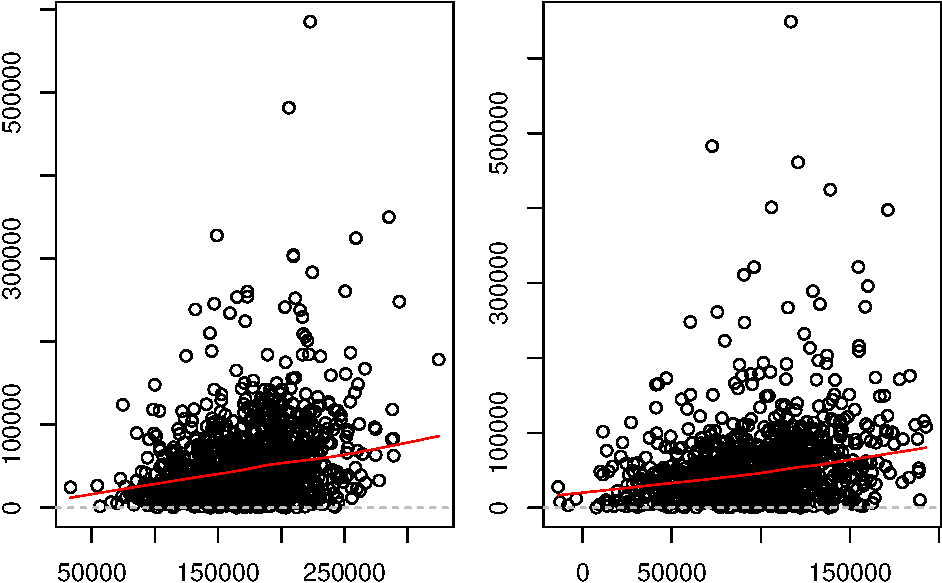
\includegraphics{Svetunkov---Svetunkov---Complex-Valued-Econometrics_files/figure-latex/heteroDiagnostics-1.pdf}
\caption{\label{fig:heteroDiagnostics}Absolute residuals vs fitted}
\end{figure}

The plots in Figure \ref{fig:heteroDiagnostics} show that the variability of residuals (and the local mean) increases with the increase of fitted values. This is a signal of the heteroscedasticity in the data. Some non-linear transformations (e.g.~taking logarithm) typically resolve the issue.

\hypertarget{assumptionsResidualsAuto}{%
\subsection{No autocorrelation in residuals}\label{assumptionsResidualsAuto}}

This assumption only applies to time series data. In case of the real-valued models, it means that the residuals in the past should not impact the ones in the future. Typically, this effect appears because of the wrong specification of the model (e.g.~the appropriate transformations are not done, or some autoregressive elements are missing). In case of the cLR, the idea is very similar, but now we are talking about complex relations between the residuals, which could arise, again, because of the wrong transformations or because of missing elements (e.g.~complex autoregression, discussed later in this book).

To diagnose this, we can analyse the autocorrelation functions. In the real-valued domain, Autocorrelation Function (ACF) and the Partial Autocorrelation Function (PACF) are typically used. In the complex-valued domain, these transform to the direct and conjugate complex ACF/PACF (or cACF/cPACF, based on the correlations discussed in Chapter \ref{correlationAnalysis}), giving an analyst four instruments instead of two \citep{ACFPACFReferences}. Furthermore, using the idea with correlation on MDS (see Section \ref{correlationMDSPearson}), we can calculate ACF/PACF based on Pearson's correlation between the complex variables reduced to real ones.

In general, the idea with direct and conjugate ACF/PACF for complex variables is similar to the one for the conventional ACF/PACF for the real ones. The complex ACF measures the correlations between the variable on observation \(t\) and the one with lag \(\tau=\{1, \dots, T\}\), where \(T\) is the maximum lag we calculate the correlation for. If we calculate the conjugate correlations, we obtain a vector of values \(\rho_{1}, \dots, \rho_{T}\) (specific formulae are discussed in Section \ref{correlationConjugate}). In case of the direct one (see Section \ref{correlationDirect}), we get a vector \(\varrho_{1}, \dots, \varrho_{T}\). In both cases the index \(j\) in subscription refers to the specific lag, so, for example, \(\rho_{1}\) will measure the conjugate autocorrelation for lag 1, i.e.~conjugate correlation between \(\underline{y}_{t}\) and \(\underline{y}_{t-1}\).

When it comes to PACF, the logic is to estimating recursively regression models of the \(\underline{y}_{t}\) from all the previous \(\underline{y}_{t-j}\) for \(j=\{1, \dots, J\}\) for each \(J\) from 1 to \(T\) and collecting respective estimates of parameters in front of \(\underline{y}_{t-J}\). This way, the coefficients are clear of the interim effects and we get a clear correlation between \(\underline{y}_{t}\) and \(\underline{y}_{t-J}\). In case of the direct complex PACF, we use the CLS, for the conjugate one we use OLS and for the Pearson's, we do MDS and then calculate the conventional PACF (see Chapter \ref{correlationAnalysis} for discussion of different correlation coefficients).

In R, there are functions \texttt{cacf()} and \texttt{cpacf()} in the \texttt{complex} package that implement respective complex ACF/PACF with a parameter \texttt{method} specifying, which of the correlations to calculate. To demonstrate how they work, we generate a data from a complex autoregressive model of order one and apply it to the data (note that for diagnostic purposes, the functions below should be applied to the residuals of the model):

\begin{Shaded}
\begin{Highlighting}[]
\CommentTok{\# Generate complex data with an autocorrelation of order 1}
\CommentTok{\# For reproducibility, fix random seed}
\KeywordTok{set.seed}\NormalTok{(}\DecValTok{41}\NormalTok{)}
\CommentTok{\# Number of observations}
\NormalTok{obs \textless{}{-}}\StringTok{ }\DecValTok{100}
\CommentTok{\# Vector of the final variable}
\NormalTok{y \textless{}{-}}\StringTok{ }\KeywordTok{vector}\NormalTok{(}\StringTok{"complex"}\NormalTok{, obs)}
\CommentTok{\# Initial values for the first observation}
\NormalTok{y[}\DecValTok{1}\NormalTok{] \textless{}{-}}\StringTok{ }\DecValTok{300} \OperatorTok{+}\StringTok{ }\NormalTok{250i}
\ControlFlowTok{for}\NormalTok{(i }\ControlFlowTok{in} \DecValTok{2}\OperatorTok{:}\NormalTok{obs)\{}
\NormalTok{    y[i] \textless{}{-}}\StringTok{ }\DecValTok{100} \OperatorTok{+}\StringTok{ }\NormalTok{200i }\OperatorTok{+}\StringTok{ }\NormalTok{(}\FloatTok{0.5} \OperatorTok{{-}}\StringTok{ }\FloatTok{0.25}\NormalTok{i) }\OperatorTok{*}\StringTok{ }\NormalTok{y[i}\DecValTok{{-}1}\NormalTok{] }\OperatorTok{+}
\StringTok{        }\KeywordTok{complex}\NormalTok{(}\DataTypeTok{real=}\KeywordTok{rnorm}\NormalTok{(}\DecValTok{1}\NormalTok{,}\DecValTok{0}\NormalTok{,}\DecValTok{10}\NormalTok{), }\DataTypeTok{imaginary=}\KeywordTok{rnorm}\NormalTok{(}\DecValTok{1}\NormalTok{,}\DecValTok{0}\NormalTok{,}\DecValTok{5}\NormalTok{))}
\NormalTok{\}}
\end{Highlighting}
\end{Shaded}

The conjugate ACF (due to its nature) is represented by a set of real values (Figure \ref{fig:complexAR1ACFConj}):

\begin{Shaded}
\begin{Highlighting}[]
\KeywordTok{cacf}\NormalTok{(y, }\DataTypeTok{method=}\StringTok{"conjugate"}\NormalTok{, }\DataTypeTok{plot=}\OtherTok{TRUE}\NormalTok{, }\DataTypeTok{main=}\StringTok{""}\NormalTok{)}
\end{Highlighting}
\end{Shaded}

\begin{figure}
\centering
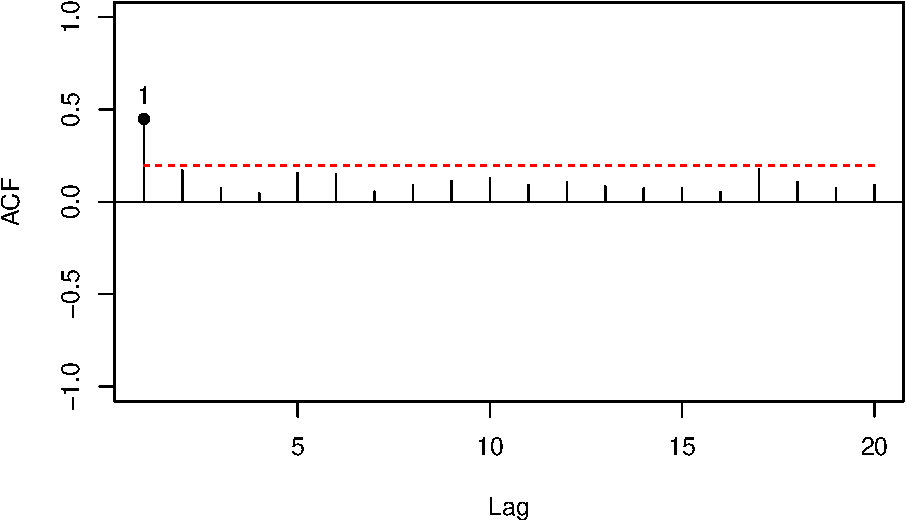
\includegraphics{Svetunkov---Svetunkov---Complex-Valued-Econometrics_files/figure-latex/complexAR1ACFConj-1.pdf}
\caption{\label{fig:complexAR1ACFConj}Conjugate complex autocorrelation function}
\end{figure}

The plot in Figure \ref{fig:complexAR1ACFConj} shows that the autocorrelation for lag one is statistically different from zero on the 5\% significance level (the latter is regulated by \texttt{level} parameter in the function). The non-rejection region on the plot is costructed based on the Folded t-distribution (which is an approximation of the square root of convolution of two Fisher distributions) and helps testing the null hypothesis that autocorrelation coefficient for each lag equals to zero (with the alternative being not equal). The value of the coefficient itself does not provide any specific information about the autoregressive relation in the data, but merely shows that the correlation between variables is mediocre.

In contrast, the conjugate PACF provides more details and shows the specific values for the real and the imaginary parts of the coefficient in the process (see Figure \ref{fig:complexAR1PACFConj}):

\begin{Shaded}
\begin{Highlighting}[]
\KeywordTok{cpacf}\NormalTok{(y, }\DataTypeTok{method=}\StringTok{"conjugate"}\NormalTok{, }\DataTypeTok{plot=}\OtherTok{TRUE}\NormalTok{, }\DataTypeTok{main=}\StringTok{""}\NormalTok{)}
\end{Highlighting}
\end{Shaded}

\begin{figure}
\centering
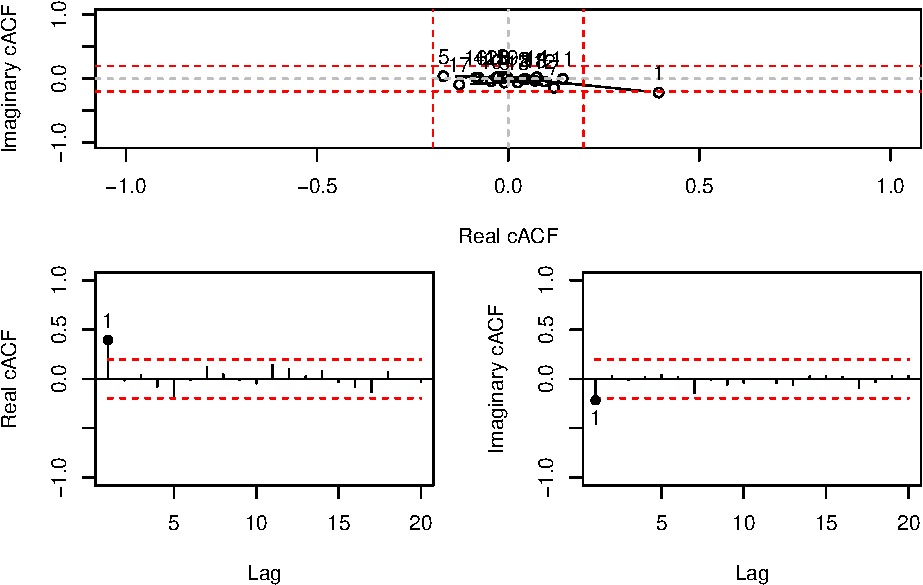
\includegraphics{Svetunkov---Svetunkov---Complex-Valued-Econometrics_files/figure-latex/complexAR1PACFConj-1.pdf}
\caption{\label{fig:complexAR1PACFConj}Conjugate complex partial autocorrelation function}
\end{figure}

Figure \ref{fig:complexAR1PACFConj} shows three plots: real vs imaginary complex ACF plot at the top and two separate plots for the real and the imaginary parts of the complex PACF at the bottom. As shown in the plots both the real and the imaginary parts of the complex coefficient are statistically different from zero on the 5\% significance level for the first lag and not significant for the rest of the lags. This agrees with the data generated process that we used. Furthermore, the real part of the cPACF is close to the true value of 0.5, while the imaginary one is close to the -0.25, which were used in the data generation.

Similarly, we can analyse the direct complex ACF of a variable, which will generate a plot similar to the ones in Figure \ref{fig:complexAR1PACFConj} (see Figure \ref{fig:complexAR1PACFDir}):

\begin{Shaded}
\begin{Highlighting}[]
\KeywordTok{cacf}\NormalTok{(y, }\DataTypeTok{method=}\StringTok{"direct"}\NormalTok{, }\DataTypeTok{plot=}\OtherTok{TRUE}\NormalTok{, }\DataTypeTok{main=}\StringTok{""}\NormalTok{)}
\end{Highlighting}
\end{Shaded}

\begin{figure}
\centering
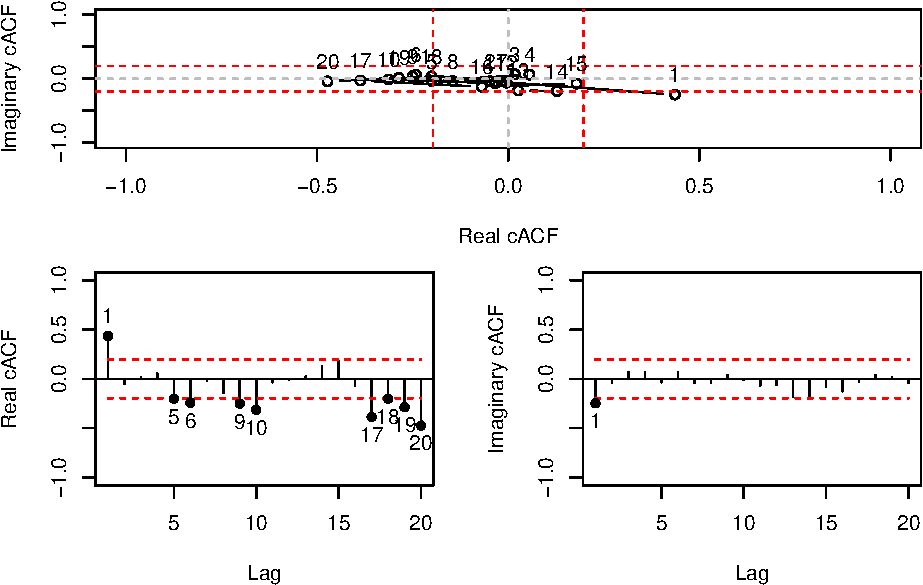
\includegraphics{Svetunkov---Svetunkov---Complex-Valued-Econometrics_files/figure-latex/complexAR1ACFDir-1.pdf}
\caption{\label{fig:complexAR1ACFDir}Direct complex autocorrelation function}
\end{figure}

While the dynamics of direct cACF is similar to the one of the conjugate cPACF, they show different things: the latter is clear of the interim relations between variables, while the former shows the specific correlations between the actual value and each of its lags. Similarly to how we did that before, we can also produce the direct cPACF (Figure \ref{fig:complexAR1PACFDir}):

\begin{Shaded}
\begin{Highlighting}[]
\KeywordTok{cpacf}\NormalTok{(y, }\DataTypeTok{method=}\StringTok{"direct"}\NormalTok{, }\DataTypeTok{plot=}\OtherTok{TRUE}\NormalTok{, }\DataTypeTok{main=}\StringTok{""}\NormalTok{)}
\end{Highlighting}
\end{Shaded}

\begin{figure}
\centering
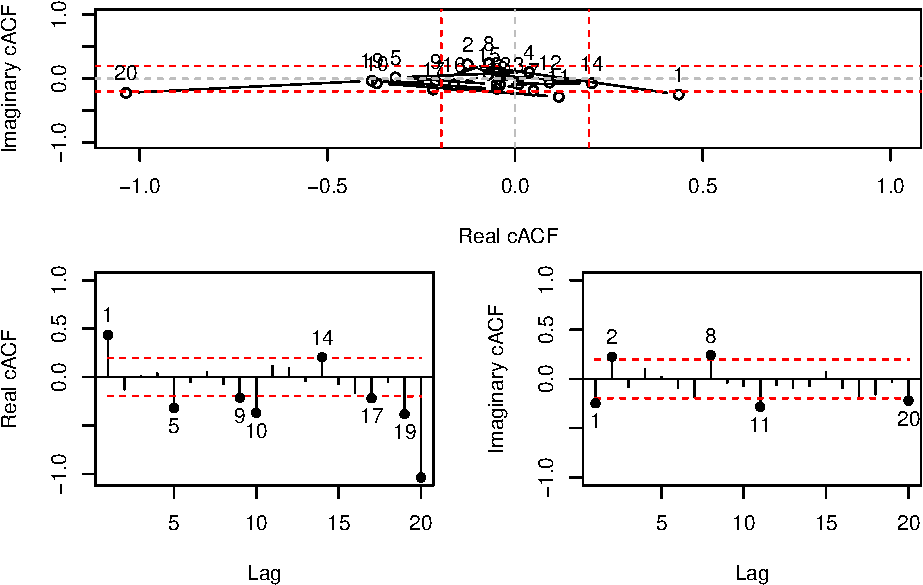
\includegraphics{Svetunkov---Svetunkov---Complex-Valued-Econometrics_files/figure-latex/complexAR1PACFDir-1.pdf}
\caption{\label{fig:complexAR1PACFDir}Direct complex partial autocorrelation function}
\end{figure}

Because we generated the data from the complex autoregressive model of order one, the cACF and cPACF give us roughly the same message: the lag one is significant on the 5\% level, while the rest of values are not. Note however that the direct cACF/cPACF shows that there are other lags that are significantly different from zero. This appears by chance and should be ignored.

Finally, we can generate ACF/PACF for the variable after its MDS transformation (Figure \ref{fig:complexAR1Pearson}):

\begin{Shaded}
\begin{Highlighting}[]
\KeywordTok{par}\NormalTok{(}\DataTypeTok{mfcol=}\KeywordTok{c}\NormalTok{(}\DecValTok{2}\NormalTok{,}\DecValTok{1}\NormalTok{), }\DataTypeTok{mar=}\KeywordTok{c}\NormalTok{(}\DecValTok{2}\NormalTok{,}\DecValTok{2}\NormalTok{,}\DecValTok{2}\NormalTok{,}\DecValTok{1}\NormalTok{))}
\KeywordTok{cacf}\NormalTok{(y, }\DataTypeTok{method=}\StringTok{"pearson"}\NormalTok{, }\DataTypeTok{plot=}\OtherTok{TRUE}\NormalTok{)}
\KeywordTok{cpacf}\NormalTok{(y, }\DataTypeTok{method=}\StringTok{"pearson"}\NormalTok{, }\DataTypeTok{plot=}\OtherTok{TRUE}\NormalTok{)}
\end{Highlighting}
\end{Shaded}

\begin{figure}
\centering
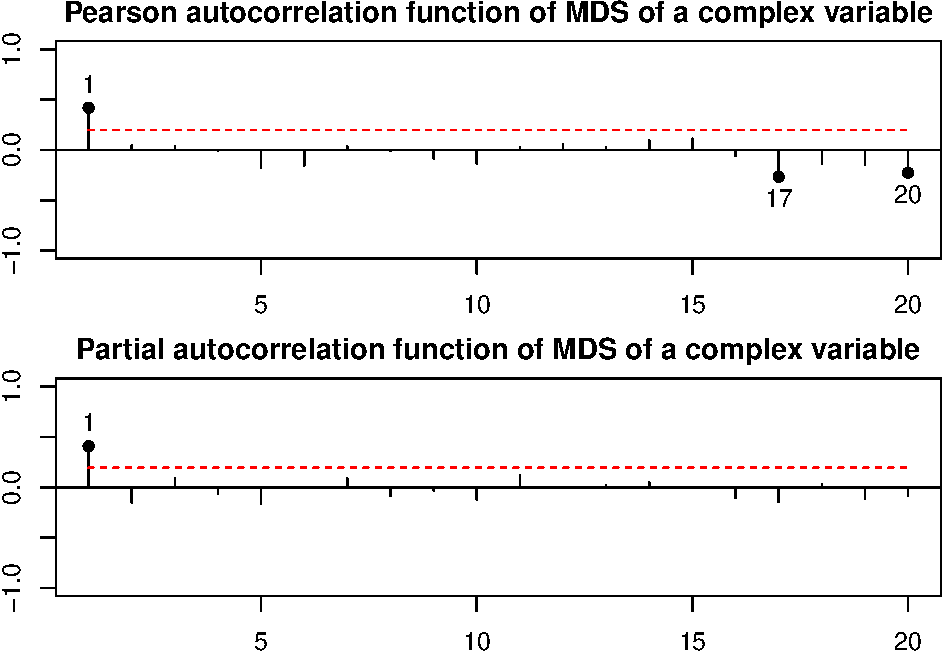
\includegraphics{Svetunkov---Svetunkov---Complex-Valued-Econometrics_files/figure-latex/complexAR1Pearson-1.pdf}
\caption{\label{fig:complexAR1Pearson}ACF and PACF of the complex variable after the MDS.}
\end{figure}

Similarly to the conjugate cACF, the plots in Figure \ref{fig:complexAR1Pearson} show that there is a significant spike for the lag one, implying that the variable is autocorrelated. However, they do not give any specific information about the value of the parameter (like conjugate and direct pACF do).

Furthermore, there is another presentation for complex ACF/PACF - in the polar coordinates one. In that case instead of plotting separate real and imaginary parts of the function, we produce the magnitude (absolute value) and the angle (argument) of the complex variables. In that presentation, the higher the magnitude is, the higher overall the value of a complex variable is. Figure \ref{fig:complexAR1Ploar} demonstrates how this looks for the conjugate cPACF:

\begin{Shaded}
\begin{Highlighting}[]
\KeywordTok{cpacf}\NormalTok{(y, }\DataTypeTok{method=}\StringTok{"conjugate"}\NormalTok{, }\DataTypeTok{plot=}\OtherTok{FALSE}\NormalTok{) }\OperatorTok{|}\ErrorTok{\textgreater{}}
\StringTok{    }\KeywordTok{plot}\NormalTok{(}\DecValTok{2}\NormalTok{)}
\end{Highlighting}
\end{Shaded}

\begin{figure}
\centering
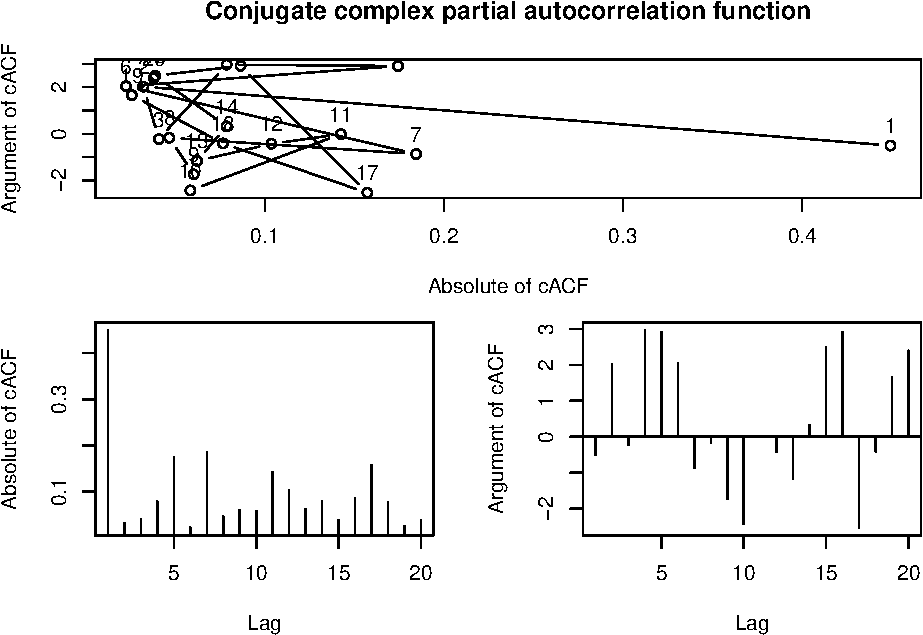
\includegraphics{Svetunkov---Svetunkov---Complex-Valued-Econometrics_files/figure-latex/complexAR1Ploar-1.pdf}
\caption{\label{fig:complexAR1Ploar}Complex ACF in polar coordinates.}
\end{figure}

The distribution of the absolute value of a bivariate normal complex variable follows Hoyt's distribution, which can be used for the confidence interval construction for the plot above. However, the derivations become complicated and we do not provide them here (we might provide them in the future editions of this monograph).

Finally, one can analyse the ACF/PACF of the separate real and imaginary parts of the residuals, thus ignoring the potential dynamics between them. The analysis in this case becomes trivial and has been discussed in many textbooks and monographs \citep[for example, see][]{SvetunkovAdam}. In R, if a model is estimated using the \texttt{clm()} function from the \texttt{complex} package, the \texttt{plot()} method supports producing ACF/PACF for each separate variable. For example, for the same model from the Subsection \ref{assumptionsSpecificationTransformation}, we have (see Figure \ref{fig:complexAR1Ploar}):

\begin{Shaded}
\begin{Highlighting}[]
\KeywordTok{par}\NormalTok{(}\DataTypeTok{mfcol=}\KeywordTok{c}\NormalTok{(}\DecValTok{2}\NormalTok{,}\DecValTok{2}\NormalTok{))}
\KeywordTok{plot}\NormalTok{(complexModel,}\DataTypeTok{which=}\KeywordTok{c}\NormalTok{(}\DecValTok{10}\NormalTok{,}\DecValTok{11}\NormalTok{))}
\end{Highlighting}
\end{Shaded}

\begin{figure}
\centering
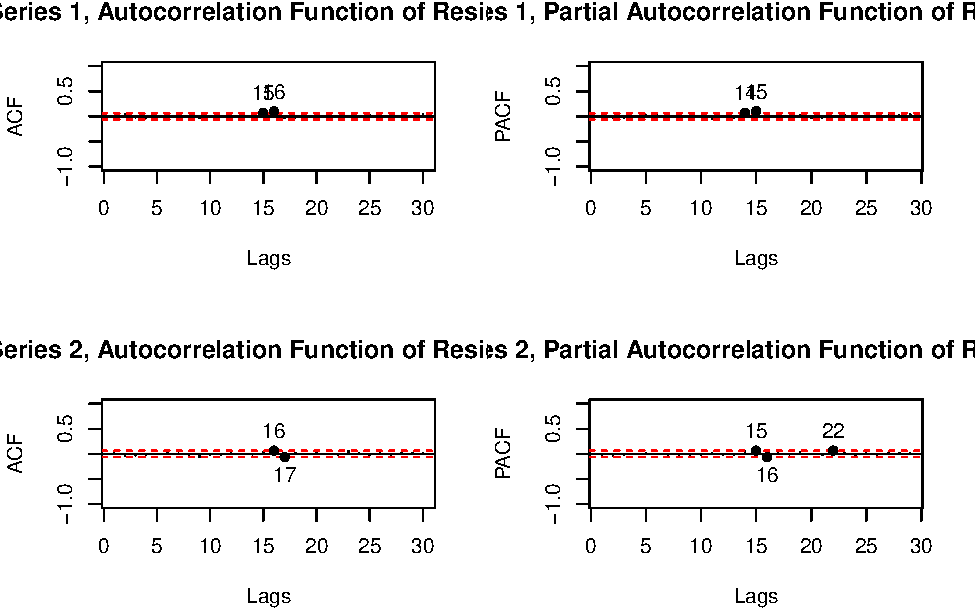
\includegraphics{Svetunkov---Svetunkov---Complex-Valued-Econometrics_files/figure-latex/complexARDiagnosticsACFPACF-1.pdf}
\caption{\label{fig:complexARDiagnosticsACFPACF}ACF/PACF for the real (Series 1) and imaginary (Series 2) parts of the complex residuals.}
\end{figure}

The residuals of this model show that there are no important lags on the 5\% significance level. The fact that there are some correlations with values lying outside of the non-rejection region can be explained by random chance. We should take such cases with a pinch of salt not to overcomplicate a model.

In addition, we can do more thorough diagnostics based on the complex ACF/PACF (as discussed above) for any complex-valued model. In that case we need to extract residuals and then apply \texttt{cacf()} or \texttt{cpacf()} functions. For example, using this code:

\begin{Shaded}
\begin{Highlighting}[]
\KeywordTok{residuals}\NormalTok{(complexModel) }\OperatorTok{|}\ErrorTok{\textgreater{}}
\StringTok{    }\KeywordTok{cacf}\NormalTok{(}\DataTypeTok{method=}\StringTok{"direct"}\NormalTok{)}
\end{Highlighting}
\end{Shaded}

After doing the diagnostics of the residuals of a cLR, we can change its form by introducing complex AR (autoregression) or MA (moving average) elements, depending on what lags seem significant on the selected level. The complex AR/MA models are outside of the scope of this monograph and are not discussed in detail here. It suffices to say that in order to construct the complex AR, one needs to generate lagged response variable and add it to the matrix with the explanatory variables. The estimation of such model should be trivial.

\hypertarget{expectation-of-residuals-is-zero}{%
\subsection{Expectation of residuals is zero}\label{expectation-of-residuals-is-zero}}

While many other assumptions can be diagnosed in one way or another, this assumption in many cases cannot be. For example, if we use OLS, the unconditional mean of the residuals will be equal to zero by design, which does not provide any useful information about the ``true'' model. However, this assumption can be analysed conditionally, e.g.~conditional on the fitted values:

\begin{equation}
    \mathrm{E}(\underline{e}_j | \underline{\mathbf{x}}_j)=0 ,
    \label{eq:residsExpectation}
\end{equation}
meaning that the expectation of complex residual conditional on the values of explanatory variables should be equal to zero. If the conditional mean is not constant and not zero, then we can conclude that some important elements were omitted in the model. In a way, the assumption becomes similar to the assumption about the omitted variables, wrong transformations, and/or autocorrelated residuals. To that extent, we do not discuss it in more detail here.

\hypertarget{residuals-follow-an-assumed-distribution}{%
\subsection{Residuals follow an assumed distribution}\label{residuals-follow-an-assumed-distribution}}

In the classical real-valued regression, this assumption is not considered to be crucial, and if a model is estimated using OLS, it typically comes to the ``residuals follow the Normal distribution''. In context of complex variables, the equivalent assumption would be that the complex residuals follow the Complex Normal distribution discussed in Subsection \ref{distributionCNorm}. If the model is formulated using matrix notations \eqref{eq:CLRSystemVectorFinal}, the assumption transforms to ``Multivariate Normal'' one, discussed in Section \ref{MVNorm}. In statistics, this assumption is typically considered as not critical in comparison with the others. This is because it can be shown that in case of OLS/CLS even when it does not hold, but all the others do, the estimates of parameters should be unbiased, efficient and consistent. However, this assumption becomes essential when prediction interval needs to be generated from the model. In that case we want to capture the uncertainty about the data correctly, and if the residuals do not follow the Normal distribution, the prediction interval will be miscalibrated.

One of the simplest ways of checking the assumption is by producing QQ-plots for each part of the complex residuals. This approach ignores the multivariate nature of the residuals (e.g.~then can be correlated), but given that each part of the c.r.v. following Complex Normal distribution is Normal as well, this should suffice for diagnostic purposes.

In R, this can be done using the following command (for the model discussed in Subsection \ref{assumptionsSpecificationTransformation}, see Figure \ref{fig:complexNormDiagnostics}):

\begin{Shaded}
\begin{Highlighting}[]
\KeywordTok{par}\NormalTok{(}\DataTypeTok{mfcol=}\KeywordTok{c}\NormalTok{(}\DecValTok{1}\NormalTok{,}\DecValTok{2}\NormalTok{))}
\KeywordTok{plot}\NormalTok{(complexModelLogs,}\DataTypeTok{which=}\DecValTok{6}\NormalTok{)}
\end{Highlighting}
\end{Shaded}

\begin{figure}
\centering
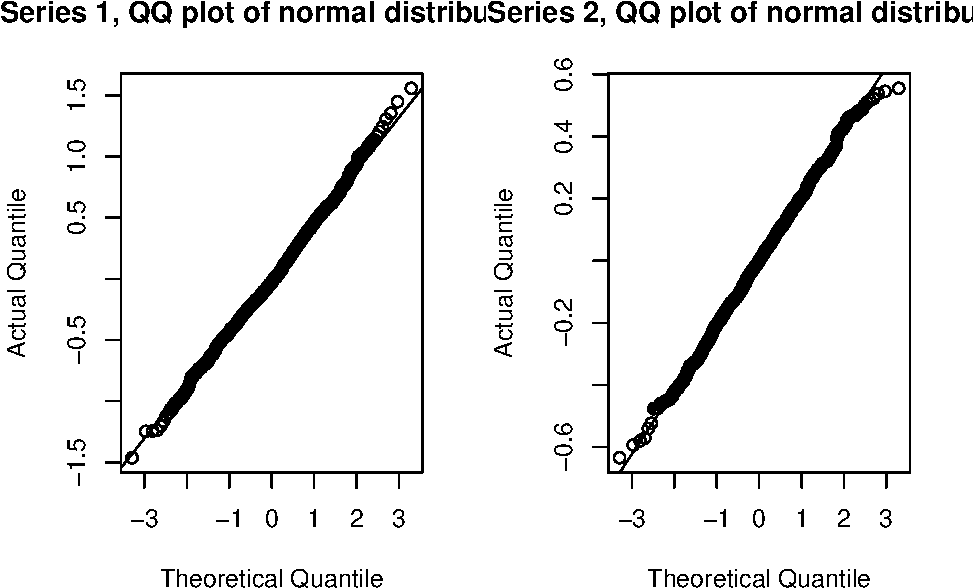
\includegraphics{Svetunkov---Svetunkov---Complex-Valued-Econometrics_files/figure-latex/complexNormDiagnostics-1.pdf}
\caption{\label{fig:complexNormDiagnostics}QQ-plots for the real (Series 1) and imaginary (Series 2) parts of the residuals.}
\end{figure}

Similarly to the conventional diagnostics related to distributional assumptions, the QQ-plots in Figure \ref{fig:complexNormDiagnostics} can be interpreted as follows. If all the points (empirical quantiles) lie on or close to the lines (theoretical quantiles) then the empirical distribuion looks similar to the theoretical one. In the example in Figure \ref{fig:complexNormDiagnostics}, we see that the points are indeed close to the lines for both real (called ``Series 1'') and imaginary (called ``Series 2'' in the plot) parts of the residuals. There is a slight deviation in the right tail of the imaginary part, but it is not substantial. Based on this diagnostics we can conclude that the residuals look Normal or at least very close to it.

\hypertarget{residuals-follow-a-circular-distribution}{%
\subsection{Residuals follow a circular distribution}\label{residuals-follow-a-circular-distribution}}

Finally, in signal processing literature, there is an assumption that residuals follow so called ``circular distribution''. This means that the covariance between the residuals equals to zero and that the variance of the real part is equal to the variance of the imaginary one. This also implies that the direct variance of residuals is equal to zero. While this might be a suitable assumption in signal processing, there is no good rationale for this to hold universally for all cLR models. In fact, the power of the cLR comes from different variances and potentially non-zero covariance between the residuals, because in that case the model can capture a complex dynamics between the parts of the complex variable. So, we suggest ignoring this assumption, especially given that it does not effect estimates of parameters of the forecasts from the model.

However, it is important to note that the used estimation methods might imply some parts of this assumption. For example, OLS minimises the sum of squared residuals of the real and imaginary parts, completely neglecting the covariance between them (see Subsection \ref{SCLREstimationOLS}). At the same time, the CLS (Subsection \ref{SCLREstimationCLS}) ignores the specific sizes of the squared residuals and focuses on making their squares equal, minimising at the same time the covariance between them. If we believe that the residuals might have a more complicated distribution (elliptic Normal) then MLE (Subsection \ref{SCLREstimationLikelihood}) might be the best option for the model estimation.

\hypertarget{explanatory-variables-are-not-correlated-with-anything-but-the-response-variable}{%
\section{Explanatory variables are not correlated with anything but the response variable}\label{explanatory-variables-are-not-correlated-with-anything-but-the-response-variable}}

The two assumptions in this group relate to the estimation of model rather than anything else:

\begin{enumerate}
\def\labelenumi{\arabic{enumi}.}
\tightlist
\item
  No endogeneity
\item
  No multicollinearity
\end{enumerate}

The first assumption comes to the idea that a linear regression model can only capture a one-directional relation, where an explanatory variable impacts the response variable. If the relation in the real life is bi-directional then the estimates of parameters of a regression model will be biased. In that case, the relation needs to be somehow made one-directional, for example by substituting the explanatory variable that causes a problem with something similar that is not impacted by the response variable. In case of the complex linear regression, the situation would be similar to the conventional one. We do not plan to discuss how to solve the problem in case of cLR in this monograph. But we believe that the methods from econometrics of real-valued models should be widely applicable here as well (e.g.~using proxies or instrumental variables).

As for the multicollinearity issue, in the real-valued statistics, it arises when least squares or maximum likelihood is used for estimation. It is, in a way, a technical issue: if the explanatory variables are linearly related it becomes difficult to split the impact of each of the explanatory variables on the response variable and thus challenging to correctly capture the relations between the explanatory variables and the response one.

In case of an OLS applied to a conventional real-valued regression model, the issue comes to inverting the matrix \(\left( {\mathbf{X}}^\prime {\mathbf{X}} \right)^{-1}\). If some of variables in \(\mathbf{X}\) are strongly linearly related, the determinant of the matrix becomes close to zero and thus the inversion becomes challenging. Even if it is still possible to invert the matrix, the estimates of parameters become inefficient because small changes in the related explanatory variables may lead to substantial changes in the inversion.

In case of cLR, the situation is similar, but with some specific features. First, it comes to the estimation methods, with the following options (as discussed in Section \ref{mlcrEstimation}):

\begin{itemize}
\tightlist
\item
  OLS: \(\underline{\boldsymbol{b}}^{OLS} = \left( \underline{\mathbf{X}}^\prime \underline{\mathbf{X}} \right)^{-1} \underline{\mathbf{X}}^\prime \underline{\mathbf{y}}\);
\item
  CLS: \(\underline{\boldsymbol{b}}^{CLS} = \left( \underline{\mathbf{X}}^\top \underline{\mathbf{X}}\right)^{-1} \underline{\mathbf{X}}^\top \underline{\mathbf{y}}\);
\item
  Likelihood: no analytical solution, comes to the minimisation of the Generalised Variance \(|\hat{\boldsymbol{\Sigma}}_\epsilon|\).
\end{itemize}

If the OLS is used for parameters estimation then a potential issue might arise from the inversion of \(\left( \underline{\mathbf{X}}^\prime \underline{\mathbf{X}}\right)^{-1}\). In one of the special cases, this comes to the conjugate covariance between variables. If it is too high in comparison to the conjugate variances, then we would face the multicollinearity issue, which would make the estimates of parameters inefficient. More generally speaking, if a complex linear regression between an explanatory variable and other explanatory variables estimated using OLS captures the relations between variables well (i.e.~having a high coefficient of determination), then we might be facing a multicollinearity problem.

Similar problems might appear in case of CLS, but they come to a slightly different inversion, \(\left( \underline{\mathbf{X}}^\top \underline{\mathbf{X}}\right)^{-1}\) and thus relates to direct covariances rather than the conjugate ones.

And when it comes to the likelihood, due to the model formulation, the conventional real-valued relations between explanatory variables should be considered when multicollinearity is suspected.

All of this means that a choice of an estimator can be dictated by the strength of the conventional Pearson's, direct and/or conjugate correlations (and more widely conventional linear model and/or complex linear model for explanatory variables estimated using OLS/CLS).

In addition to the estimation issues, there might be some related to the calculation of the covariance matrix of parameters (discussed in Section \ref{MCLRInference}), where we need both direct and conjugate covariance matrices:

\begin{itemize}
\tightlist
\item
  OLS:

  \begin{itemize}
  \tightlist
  \item
    Conjugate covariance matrix: \(\mathrm{V}\left( \underline{\boldsymbol{b}}^{\text{OLS}} \right) = \left( \underline{\mathbf{X}}^\prime \underline{\mathbf{X}} \right)^{-1} \underline{\mathbf{X}}^\prime \tilde{\underline{\mathbf{X}}} \left( {\underline{\mathbf{X}}}^\top \tilde{\underline{\mathbf{X}}} \right)^{-1 \prime} \sigma_{\underline{\epsilon}}^2\)
  \item
    Direct covariance matrix: \(\mathcal{V}\left( \underline{\boldsymbol{b}}^{\text{OLS}} \right) = \left( \underline{\mathbf{X}}^\prime \underline{\mathbf{X}} \right)^{-1} \varsigma_{\underline{\epsilon}}^2\);
  \end{itemize}
\item
  CLS:

  \begin{itemize}
  \tightlist
  \item
    Conjugate covariance matrix: \(\mathrm{V}\left( \underline{\boldsymbol{b}}^{\text{CLS}} \right) = \left( \underline{\mathbf{X}}^\top \underline{\mathbf{X}} \right)^{-1} \underline{\mathbf{X}}^\top \tilde{\underline{\mathbf{X}}} \left( {\underline{\mathbf{X}}}^\prime \tilde{\underline{\mathbf{X}}} \right)^{-1 \top} \sigma_{\underline{\epsilon}}^2\)
  \item
    Direct covariance matrix: \(\mathcal{V}\left( \underline{\boldsymbol{b}}^{\text{CLS}} \right) = \left( \underline{\mathbf{X}}^\top \underline{\mathbf{X}} \right)^{-1} \varsigma_{\underline{\epsilon}}^2\);
  \end{itemize}
\item
  Likelihood: no closed form, comes to calculating Hessian, which involves the inversion of a matrix based on the matrix of explanatory variables.
\end{itemize}

In this case, the linear relation between explanatory variables (in one form or the other) will impact the elements of the final covariance matrix inflating them and thus leading to the higher uncertainty of the estimates of parameters. Given that we need both direct and conjugate covariance matrices for the calculation of the standard errors of the individual parameters, the choice of estimation method would not resolve the multicollinearity issue. We can expect that the standard errors of parameters will be higher than in the situation without the multicollinearity, no matter what estimation method we use.

Note that the standard issues that arise in conventional regression analysis due to linear relation between variables, might not apply to the cLR. For example, if a real part of one variable is strongly correlated with either a real or an imaginary part of the other one, the model might still be estimable and would not suffer from multicollinearity. The effect of multicollinearity in cLR is much more pronounced, when the complex variables are linearly related, rather than their separate parts.

The diagnostics of the multicollinearity in cLR can be done by calculating the correlation matrix between the explanatory variables to see whether there is a strongly related couple of them. Given the nature of the model, this means that we might need to estimate and analyse the direct and conjugate correlation matrices together with the conventional one after transforming the complex variables to the vector of real ones.

\hypertarget{demonstration-in-r-3}{%
\subsection{Demonstration in R}\label{demonstration-in-r-3}}

For demonstration purposes we generate data from a model:
\begin{equation*}
    \underline{y} = \underline{\beta}_0 + \underline{\beta}_1 \underline{x}_{1} + \underline{\beta}_2 \underline{x}_{2} + \underline{\epsilon}
\end{equation*}
for several scenarios:

\begin{enumerate}
\def\labelenumi{\arabic{enumi}.}
\tightlist
\item
  \(\underline{x}_{1}\) is strongly correlated with \(\underline{x}_{2}\);
\item
  \(\mathcal{R}\left(\underline{x}_{1}\right)\) is strongly correlated with \(\mathcal{R}\left(\underline{x}_{2}\right)\);
\item
  \(\mathcal{R}\left(\underline{x}_{1}\right)\) is strongly correlated with \(\mathcal{I}\left(\underline{x}_{2}\right)\).
\end{enumerate}

These three cases should cover the main possible issues in the model, and we will see what different estimators give in terms of parameters and their standard errors. We do not conduct a proper simulation experiment, but instead focus on a demonstration for one data series.

The R code below creates three datasets for the three respective scenarios (the coefficients have been selected arbitrarily):

\begin{Shaded}
\begin{Highlighting}[]
\KeywordTok{set.seed}\NormalTok{(}\DecValTok{41}\NormalTok{)}
\CommentTok{\# Sample size}
\NormalTok{obs \textless{}{-}}\StringTok{ }\DecValTok{100}
\CommentTok{\# Generate parameters}
\NormalTok{b0 \textless{}{-}}\StringTok{ }\DecValTok{100} \OperatorTok{{-}}\StringTok{ }\NormalTok{150i}
\NormalTok{b1 \textless{}{-}}\StringTok{ }\FloatTok{2.5} \OperatorTok{+}\StringTok{ }\FloatTok{1.5}\NormalTok{i}
\NormalTok{b2 \textless{}{-}}\StringTok{ }\FloatTok{1.5} \OperatorTok{{-}}\StringTok{ }\FloatTok{0.75}\NormalTok{i}
\NormalTok{a1 \textless{}{-}}\StringTok{ }\FloatTok{1.3} \OperatorTok{+}\StringTok{ }\FloatTok{1.5}\NormalTok{i}
\CommentTok{\# Create the explanatory variables}
\NormalTok{x1 \textless{}{-}}\StringTok{ }\KeywordTok{rcnorm}\NormalTok{(obs, }\DataTypeTok{mu=}\DecValTok{100}\OperatorTok{+}\NormalTok{50i, }\DataTypeTok{sigma2=}\DecValTok{125}\NormalTok{, }\DataTypeTok{varsigma2=}\DecValTok{75}\NormalTok{)}
\CommentTok{\# Generate error term from the complex normal distribution}
\NormalTok{e \textless{}{-}}\StringTok{ }\KeywordTok{rcnorm}\NormalTok{(obs, }\DataTypeTok{mu=}\DecValTok{0}\NormalTok{, }\DataTypeTok{sigma2=}\DecValTok{40}\OperatorTok{\^{}}\DecValTok{2}\NormalTok{, }\DataTypeTok{varsigma2=}\OperatorTok{{-}}\DecValTok{500}\NormalTok{)}
\CommentTok{\# The second variable}

\CommentTok{\#\# Scenario 1}
\NormalTok{x2 \textless{}{-}}\StringTok{ }\NormalTok{a1}\OperatorTok{*}\NormalTok{x1 }\OperatorTok{+}\StringTok{ }\KeywordTok{rnorm}\NormalTok{(obs,}\DecValTok{0}\NormalTok{,}\DecValTok{1}\NormalTok{)}
\CommentTok{\# Generate the response variable}
\NormalTok{y \textless{}{-}}\StringTok{ }\NormalTok{b0 }\OperatorTok{+}\StringTok{ }\NormalTok{b1 }\OperatorTok{*}\StringTok{ }\NormalTok{x1 }\OperatorTok{+}\StringTok{ }\NormalTok{b2 }\OperatorTok{*}\StringTok{ }\NormalTok{x2 }\OperatorTok{+}\StringTok{ }\NormalTok{e}
\CommentTok{\# Form a data frame with the variables}
\NormalTok{data1 \textless{}{-}}\StringTok{ }\KeywordTok{data.frame}\NormalTok{(}\DataTypeTok{y=}\NormalTok{y,}\DataTypeTok{x1=}\NormalTok{x1,}\DataTypeTok{x2=}\NormalTok{x2)}

\CommentTok{\#\# Scenario 2}
\NormalTok{x2 \textless{}{-}}\StringTok{ }\KeywordTok{complex}\NormalTok{(}\DataTypeTok{real=}\KeywordTok{Re}\NormalTok{(x1)}\OperatorTok{*}\KeywordTok{Re}\NormalTok{(a1) }\OperatorTok{+}\StringTok{ }\KeywordTok{rnorm}\NormalTok{(obs,}\DecValTok{0}\NormalTok{,}\DecValTok{1}\NormalTok{),}
              \DataTypeTok{imaginary=}\KeywordTok{rnorm}\NormalTok{(obs,}\DecValTok{10}\NormalTok{,}\DecValTok{5}\NormalTok{))}
\CommentTok{\# Generate the response variable}
\NormalTok{y \textless{}{-}}\StringTok{ }\NormalTok{b0 }\OperatorTok{+}\StringTok{ }\NormalTok{b1 }\OperatorTok{*}\StringTok{ }\NormalTok{x1 }\OperatorTok{+}\StringTok{ }\NormalTok{b2 }\OperatorTok{*}\StringTok{ }\NormalTok{x2 }\OperatorTok{+}\StringTok{ }\NormalTok{e}
\CommentTok{\# Form a data frame with the variables}
\NormalTok{data2 \textless{}{-}}\StringTok{ }\KeywordTok{data.frame}\NormalTok{(}\DataTypeTok{y=}\NormalTok{y,}\DataTypeTok{x1=}\NormalTok{x1,}\DataTypeTok{x2=}\NormalTok{x2)}

\CommentTok{\#\# Scenario 3}
\NormalTok{x2 \textless{}{-}}\StringTok{ }\KeywordTok{complex}\NormalTok{(}\DataTypeTok{real=}\KeywordTok{rnorm}\NormalTok{(obs,}\DecValTok{10}\NormalTok{,}\DecValTok{5}\NormalTok{),}
              \DataTypeTok{imaginary=}\KeywordTok{Re}\NormalTok{(x1)}\OperatorTok{*}\KeywordTok{Re}\NormalTok{(a1) }\OperatorTok{+}\StringTok{ }\KeywordTok{rnorm}\NormalTok{(obs,}\DecValTok{0}\NormalTok{,}\DecValTok{1}\NormalTok{))}
\CommentTok{\# Generate the response variable}
\NormalTok{y \textless{}{-}}\StringTok{ }\NormalTok{b0 }\OperatorTok{+}\StringTok{ }\NormalTok{b1 }\OperatorTok{*}\StringTok{ }\NormalTok{x1 }\OperatorTok{+}\StringTok{ }\NormalTok{b2 }\OperatorTok{*}\StringTok{ }\NormalTok{x2 }\OperatorTok{+}\StringTok{ }\NormalTok{e}
\CommentTok{\# Form a data frame with the variables}
\NormalTok{data3 \textless{}{-}}\StringTok{ }\KeywordTok{data.frame}\NormalTok{(}\DataTypeTok{y=}\NormalTok{y,}\DataTypeTok{x1=}\NormalTok{x1,}\DataTypeTok{x2=}\NormalTok{x2)}
\end{Highlighting}
\end{Shaded}

\hypertarget{scenario-1}{%
\subsubsection*{Scenario 1}\label{scenario-1}}
\addcontentsline{toc}{subsubsection}{Scenario 1}

First, we do diagnostics based on correlation matrices that we discussed earlier in this section, including conjugate, direct and MDS-based correlations and the conventional covariance matrix of parameters.

We start with the conjugate complex correlation matrix:

\begin{Shaded}
\begin{Highlighting}[]
\KeywordTok{ccor}\NormalTok{(data1,}\DataTypeTok{method=}\StringTok{"conjugate"}\NormalTok{) }\OperatorTok{|}\ErrorTok{\textgreater{}}\StringTok{ }\KeywordTok{round}\NormalTok{(}\DecValTok{3}\NormalTok{)}
\end{Highlighting}
\end{Shaded}

\begin{verbatim}
##        y    x1    x2
## y  1.000 0.855 0.853
## x1 0.855 1.000 0.999
## x2 0.853 0.999 1.000
\end{verbatim}

The output above shows that \(\underline{x}_{1}\) is strongly correlated with \(\underline{x}_{2}\) - the correlation coefficient between them is 0.999. This agrees with how we generated the data, and we can expect issues when estimating the model and/or generating the standard errors of parameters.

The second output is for the direct complex correlation matrix:

\begin{Shaded}
\begin{Highlighting}[]
\KeywordTok{ccor}\NormalTok{(data1,}\DataTypeTok{method=}\StringTok{"direct"}\NormalTok{) }\OperatorTok{|}\ErrorTok{\textgreater{}}\StringTok{ }\KeywordTok{round}\NormalTok{(}\DecValTok{3}\NormalTok{)}
\end{Highlighting}
\end{Shaded}

\begin{verbatim}
##               y           x1            x2
## y  1.000+0.000i 1.001-0.081i  0.998-0.078i
## x1 1.001-0.081i 1.000+0.000i  1.000+0.002i
## x2 0.998-0.078i 1.000+0.002i -1.000+0.000i
\end{verbatim}

While some correlation coefficients in the output above are hard to interpret (because some of them are above one), the real part of the one between the explanatory variables equals to one (after rounding), which also indicates a strong relation between them.

We also calculate Pearson's correlation matrix for the MDS-transformed complex variables to get another look at the problem:

\begin{Shaded}
\begin{Highlighting}[]
\KeywordTok{ccor}\NormalTok{(data1,}\DataTypeTok{method=}\StringTok{"pearson"}\NormalTok{) }\OperatorTok{|}\ErrorTok{\textgreater{}}\StringTok{ }\KeywordTok{round}\NormalTok{(}\DecValTok{3}\NormalTok{)}
\end{Highlighting}
\end{Shaded}

\begin{verbatim}
##        y    x1    x2
## y  1.000 0.897 0.895
## x1 0.897 1.000 0.999
## x2 0.895 0.999 1.000
\end{verbatim}

And as we can see from the output above, the explanatory variables \(\underline{x}_{1}\) and \(\underline{x}_{2}\) are indeed strongly linearly related.

Finally, we calculate the covariance matrix of parameters between individual variables:

\begin{Shaded}
\begin{Highlighting}[]
\KeywordTok{covar}\NormalTok{(data1) }\OperatorTok{|}\ErrorTok{\textgreater{}}\StringTok{ }\KeywordTok{cov2cor}\NormalTok{() }\OperatorTok{|}\ErrorTok{\textgreater{}}\StringTok{ }\KeywordTok{round}\NormalTok{(}\DecValTok{3}\NormalTok{)}
\end{Highlighting}
\end{Shaded}

\begin{verbatim}
##         y_r   y_i   x1_r   x1_i   x2_r  x2_i
## y_r   1.000 0.389  0.888 -0.211  0.856 0.719
## y_i   0.389 1.000  0.524  0.553  0.149 0.713
## x1_r  0.888 0.524  1.000 -0.017  0.850 0.905
## x1_i -0.211 0.553 -0.017  1.000 -0.537 0.411
## x2_r  0.856 0.149  0.850 -0.537  1.000 0.547
## x2_i  0.719 0.713  0.905  0.411  0.547 1.000
\end{verbatim}

If shows that there is a strong correlation between \(\mathcal{R}\left(\underline{x}_{1}\right)\) and \(\mathcal{R}\left(\underline{x}_{2}\right)\) and \(\mathcal{I}\left(\underline{x}_{2}\right)\), while the correlation between the imaginary part of \(\underline{x}_{1}\) with the other variables is not as strong.

All of the outputs above tell us that if we want to fit the cLR, we will face difficulties due to the strong multicollinearity caused by the strong correlation between the explanatory variables. We estimate the model using the three different methods and produce their summary outputs. We start with OLS:

\begin{Shaded}
\begin{Highlighting}[]
\KeywordTok{clm}\NormalTok{(y}\OperatorTok{\textasciitilde{}}\NormalTok{., data1, }\DataTypeTok{loss=}\StringTok{"OLS"}\NormalTok{) }\OperatorTok{|}\ErrorTok{\textgreater{}}
\StringTok{    }\KeywordTok{summary}\NormalTok{()}
\end{Highlighting}
\end{Shaded}

\begin{verbatim}
## Complex Linear Regression estimated via clm()
## Response variable: y
## Loss function used in estimation: OLS
## Coefficients:
##                Estimate Std. Error Lower 2.5% Upper 97.5%  
## (Intercept)_r   81.2499    27.8800    25.9158    136.5840 *
## (Intercept)_i -162.3298    35.2247  -232.2410    -92.4185 *
## x1_r             4.2390     5.7400    -7.1532     15.6313  
## x1_i             8.9223     7.2521    -5.4712     23.3157  
## x2_r            -1.8366     2.8949    -7.5822      3.9091  
## x2_i            -2.6157     3.6576    -9.8750      4.6436  
## 
## Error covariance matrix:
##          e_r       e_i
## e_r 687.7480  108.1091
## e_i 108.1091 1097.8374
## 
## Sample size: 100
## Number of estimated parameters: 3
## Number of degrees of freedom: 97
\end{verbatim}

The output above shows that the estimates of parameters are wrong: the complex parameter for the first variable should be \(2.5 + 1.5i\), while for the second one should be \(1.5 - 0.75i\). Furthermore, the standard errors of parameters are high, leading to the high uncertainty about the parameters, so that we cannot be sure whether the true effect is positive or negative for the estimated model.

The CLS gives a very similar picture:

\begin{Shaded}
\begin{Highlighting}[]
\KeywordTok{clm}\NormalTok{(y}\OperatorTok{\textasciitilde{}}\NormalTok{., data1, }\DataTypeTok{loss=}\StringTok{"CLS"}\NormalTok{) }\OperatorTok{|}\ErrorTok{\textgreater{}}
\StringTok{    }\KeywordTok{summary}\NormalTok{()}
\end{Highlighting}
\end{Shaded}

\begin{verbatim}
## Complex Linear Regression estimated via clm()
## Response variable: y
## Loss function used in estimation: CLS
## Coefficients:
##                Estimate Std. Error Lower 2.5% Upper 97.5%  
## (Intercept)_r   89.0089    54.0839   -18.3327    196.3505  
## (Intercept)_i -198.3455    61.3562  -320.1206    -76.5704 *
## x1_r             4.3945     6.2816    -8.0728     16.8617  
## x1_i             8.8479     6.8397    -4.7271     22.4228  
## x2_r            -1.7130     2.9266    -7.5214      4.0955  
## x2_i            -2.4582     3.6720    -9.7461      4.8297  
## 
## Error covariance matrix:
##          e_r       e_i
## e_r 696.9762  106.4108
## e_i 106.4108 1101.1012
## 
## Sample size: 100
## Number of estimated parameters: 3
## Number of degrees of freedom: 97
\end{verbatim}

However, we should note that the standard errors of parameters are in some cases higher than in the OLS, but not everywhere. For example, the parameter for \(\mathcal{I}\left(\underline{x}_{1}\right)\) estimated using CLS has a lower standard error than in the case of OLS. Nonetheless, the estimates of parameters are clearly biased and not efficient.

Finally, we estimate the model using likelihood:

\begin{Shaded}
\begin{Highlighting}[]
\KeywordTok{clm}\NormalTok{(y}\OperatorTok{\textasciitilde{}}\NormalTok{., data1, }\DataTypeTok{loss=}\StringTok{"likelihood"}\NormalTok{) }\OperatorTok{|}\ErrorTok{\textgreater{}}
\StringTok{    }\KeywordTok{summary}\NormalTok{()}
\end{Highlighting}
\end{Shaded}

\begin{verbatim}
## Complex Linear Regression estimated via clm()
## Response variable: y
## Loss function used in estimation: likelihood
## Coefficients:
##                Estimate Std. Error Lower 2.5% Upper 97.5%  
## (Intercept)_r   81.2499    28.0973    25.4734    137.0263 *
## (Intercept)_i -161.9716    35.5009  -232.4450    -91.4981 *
## x1_r             4.2390     5.7847    -7.2443     15.7224  
## x1_i             8.9223     7.3090    -5.5869     23.4314  
## x2_r            -1.8383     2.9175    -7.6299      3.9533  
## x2_i            -2.6157     3.6863    -9.9334      4.7020  
## 
## Error covariance matrix:
##          e_r       e_i
## e_r 698.5102  109.8689
## e_i 109.8689 1115.1225
## 
## Sample size: 100
## Number of estimated parameters: 4.5
## Number of degrees of freedom: 95.5
## Information criteria:
##      AIC     AICc      BIC     BICc 
## 1922.373 1922.897 1934.096 1935.303
\end{verbatim}

Because we generated the data with the uncorrelated errors, the output of the likelihood is very similar to the one from the OLS. In the other situation it might have produced different estimates of parameters.

All of the above happened because of the strong multicollinearity in the data: the complex variables \(\underline{x}_{1}\) and \(\underline{x}_{2}\) were strongly correlated by design, which caused the aforementioned issues.

The Scenario 1 demonstrates the behaviour of estimators as expected: we would not expect to estimate the models successfully, when the complex variables are so strongly correlated.

As a side note, in this scenario, we would not be able to get efficient and unbiased estimates of parameters for the individual real-valued models for \(\mathcal{R}\left(\underline{y}\right)\) and \(\mathcal{I}\left(\underline{y}\right)\) with this data, because the covariance matrix with individual variables demonstrated a high correlation between \(\mathcal{R}\left(\underline{x}_1\right)\) and \(\mathcal{I}\left(\underline{x}_2\right)\).

\hypertarget{scenario-2}{%
\subsubsection*{Scenario 2}\label{scenario-2}}
\addcontentsline{toc}{subsubsection}{Scenario 2}

In this scenario, we have strong correlation between real parts of explanatory variables, but not between the complex ones. We would expect the real-valued regression to fail in this case, but the cLR might still be estimable. We start the demonstration with the same set of outputs as before:

\begin{Shaded}
\begin{Highlighting}[]
\KeywordTok{ccor}\NormalTok{(data2,}\DataTypeTok{method=}\StringTok{"conjugate"}\NormalTok{) }\OperatorTok{|}\ErrorTok{\textgreater{}}\StringTok{ }\KeywordTok{round}\NormalTok{(}\DecValTok{3}\NormalTok{)}
\end{Highlighting}
\end{Shaded}

\begin{verbatim}
##        y    x1    x2
## y  1.000 0.723 0.687
## x1 0.723 1.000 0.791
## x2 0.687 0.791 1.000
\end{verbatim}

The conjugate correlation above shows that there is a linear relation between \(\underline{x}_{1}\) and \(\underline{x}_{2}\), but it is not sever, so we should be able to estimate the model and get reasonable estimates of parameters.

\begin{Shaded}
\begin{Highlighting}[]
\KeywordTok{ccor}\NormalTok{(data2,}\DataTypeTok{method=}\StringTok{"direct"}\NormalTok{) }\OperatorTok{|}\ErrorTok{\textgreater{}}\StringTok{ }\KeywordTok{round}\NormalTok{(}\DecValTok{3}\NormalTok{)}
\end{Highlighting}
\end{Shaded}

\begin{verbatim}
##               y           x1           x2
## y  1.000+0.000i 1.152-0.146i 1.219-0.062i
## x1 1.152-0.146i 1.000+0.000i 1.330+0.012i
## x2 1.219-0.062i 1.330+0.012i 1.000+0.000i
\end{verbatim}

The direct correlation agrees with the conjugate one in general, but the fact that the correlation between \(\underline{x}_{1}\) and \(\underline{x}_{2}\) has the real part above one, implies that the relation between the variables is stronger than expected by the previous output.

\begin{Shaded}
\begin{Highlighting}[]
\KeywordTok{ccor}\NormalTok{(data2,}\DataTypeTok{method=}\StringTok{"pearson"}\NormalTok{) }\OperatorTok{|}\ErrorTok{\textgreater{}}\StringTok{ }\KeywordTok{round}\NormalTok{(}\DecValTok{3}\NormalTok{)}
\end{Highlighting}
\end{Shaded}

\begin{verbatim}
##        y    x1    x2
## y  1.000 0.854 0.858
## x1 0.854 1.000 0.997
## x2 0.858 0.997 1.000
\end{verbatim}

Pearson's correlations on the MDS variables shows that there is a very strong relation between \(\underline{x}_{1}\) and \(\underline{x}_{2}\), although we cannot say for sure what causes it.

\begin{Shaded}
\begin{Highlighting}[]
\KeywordTok{covar}\NormalTok{(data2) }\OperatorTok{|}\ErrorTok{\textgreater{}}\StringTok{ }\KeywordTok{cov2cor}\NormalTok{() }\OperatorTok{|}\ErrorTok{\textgreater{}}\StringTok{ }\KeywordTok{round}\NormalTok{(}\DecValTok{3}\NormalTok{)}
\end{Highlighting}
\end{Shaded}

\begin{verbatim}
##         y_r   y_i   x1_r   x1_i   x2_r   x2_i
## y_r   1.000 0.151  0.857 -0.135  0.861 -0.012
## y_i   0.151 1.000  0.161  0.337  0.163  0.112
## x1_r  0.857 0.161  1.000 -0.017  0.997 -0.016
## x1_i -0.135 0.337 -0.017  1.000 -0.015 -0.136
## x2_r  0.861 0.163  0.997 -0.015  1.000 -0.022
## x2_i -0.012 0.112 -0.016 -0.136 -0.022  1.000
\end{verbatim}

Finally, as expected, the correlations between the specific parts of variables shows that \(\mathcal{R}\left(\underline{x}_1\right)\) and \(\mathcal{R}\left(\underline{x}_2\right)\) have almost functional relation. This might mean that we could face difficulties estimating the model.

The model estimated using OLS produces the following output:

\begin{Shaded}
\begin{Highlighting}[]
\KeywordTok{clm}\NormalTok{(y}\OperatorTok{\textasciitilde{}}\NormalTok{., data2, }\DataTypeTok{loss=}\StringTok{"OLS"}\NormalTok{) }\OperatorTok{|}\ErrorTok{\textgreater{}}
\StringTok{    }\KeywordTok{summary}\NormalTok{()}
\end{Highlighting}
\end{Shaded}

\begin{verbatim}
## Complex Linear Regression estimated via clm()
## Response variable: y
## Loss function used in estimation: OLS
## Coefficients:
##                Estimate Std. Error Lower 2.5% Upper 97.5%  
## (Intercept)_r   58.7490    32.3010    -5.3596    122.8575  
## (Intercept)_i -182.8910    41.0770  -264.4174   -101.3646 *
## x1_r             2.7010     0.3975     1.9121      3.4900 *
## x1_i             0.9558     0.5055    -0.0475      1.9591  
## x2_r             1.5106     0.3245     0.8666      2.1546 *
## x2_i            -0.1824     0.4126    -1.0014      0.6365  
## 
## Error covariance matrix:
##          e_r       e_i
## e_r 678.7893  108.4556
## e_i 108.4556 1097.7400
## 
## Sample size: 100
## Number of estimated parameters: 3
## Number of degrees of freedom: 97
\end{verbatim}

The parameters seem to be less efficient than they would have been without the strong correlation between parts of explanatory variables, but notably all signs are correct and the specific values are not too far from the ones used in the data generation (\(\underline{\beta}_1=2.5+1.5i\), \(\underline{\beta}_2=1.5-0.75i\)). But it would be interesting to compare the output from OLS with the one from the CLS:

\begin{Shaded}
\begin{Highlighting}[]
\KeywordTok{clm}\NormalTok{(y}\OperatorTok{\textasciitilde{}}\NormalTok{., data2, }\DataTypeTok{loss=}\StringTok{"CLS"}\NormalTok{) }\OperatorTok{|}\ErrorTok{\textgreater{}}
\StringTok{    }\KeywordTok{summary}\NormalTok{()}
\end{Highlighting}
\end{Shaded}

\begin{verbatim}
## Complex Linear Regression estimated via clm()
## Response variable: y
## Loss function used in estimation: CLS
## Coefficients:
##                Estimate Std. Error Lower 2.5% Upper 97.5%  
## (Intercept)_r   46.5476    37.5007   -27.8808    120.9760  
## (Intercept)_i -175.9491    47.1085  -269.4465    -82.4518 *
## x1_r             2.8511     0.5146     1.8299      3.8724 *
## x1_i             0.9655     0.4235     0.1250      1.8059 *
## x2_r             1.4826     0.4179     0.6531      2.3120 *
## x2_i            -0.2975     0.3625    -1.0170      0.4221  
## 
## Error covariance matrix:
##          e_r       e_i
## e_r 681.2265  110.0717
## e_i 110.0717 1099.2501
## 
## Sample size: 100
## Number of estimated parameters: 3
## Number of degrees of freedom: 97
\end{verbatim}

The estimates of parameters in CLS are similar to the OLS, but there are several interesting observations:

\begin{enumerate}
\def\labelenumi{\arabic{enumi}.}
\tightlist
\item
  The standard errors for the real parts of parameters in CLS are higher than the similar estimates in OLS;
\item
  The standard errors for the imaginary parts of parameters in CLS are lower than the respective ones in OLS;
\item
  The imaginary parts of the parameters are closer to the true ones for the CLS, while the real ones are closer to the true ones in OLS.
\end{enumerate}

But overall, both methods produce biased, potentially not too efficient, but reasonable estimates of parameters. This was not the case for the Scenario 1.

We skip the likelihood estimation, because for our DGP, it would produce estimates similar to the ones from OLS due to the zero correlation between the real and imaginary parts of the error term.

Finally, we should note that the conventional real-valued regression would not be estimable in this situation due to the high correlation between some parts of the variables. This demonstrates the difference between the cLR and the LR.

\hypertarget{scenario-3}{%
\subsubsection*{Scenario 3}\label{scenario-3}}
\addcontentsline{toc}{subsubsection}{Scenario 3}

As a reminder, in the Scenario 3 the real part of \(\underline{x}_{1}\) is strongly correlated with the imaginary one of \(\underline{x}_{2}\). We skip the correlation coefficients because arguably they will provide the information similar to the one from Scenario 2, showing the strong correlation between \(\mathcal{R}\left(\underline{x}_{1}\right)\) and \(\mathcal{I}\left(\underline{x}_{2}\right)\) as intended.

The OLS estimate of the model gives:

\begin{Shaded}
\begin{Highlighting}[]
\KeywordTok{clm}\NormalTok{(y}\OperatorTok{\textasciitilde{}}\NormalTok{., data3, }\DataTypeTok{loss=}\StringTok{"OLS"}\NormalTok{) }\OperatorTok{|}\ErrorTok{\textgreater{}}
\StringTok{    }\KeywordTok{summary}\NormalTok{()}
\end{Highlighting}
\end{Shaded}

\begin{verbatim}
## Complex Linear Regression estimated via clm()
## Response variable: y
## Loss function used in estimation: OLS
## Coefficients:
##                Estimate Std. Error Lower 2.5% Upper 97.5%  
## (Intercept)_r   51.9756    36.0017   -19.4778    123.4290  
## (Intercept)_i -174.5119    45.5491  -264.9143    -84.1095 *
## x1_r             2.6536     0.3928     1.8740      3.4331 *
## x1_i             1.0941     0.4969     0.1078      2.0803 *
## x2_r             1.9229     0.3179     1.2921      2.5538 *
## x2_i            -0.8264     0.4022    -1.6246     -0.0282 *
## 
## Error covariance matrix:
##          e_r      e_i
## e_r 686.3546  114.530
## e_i 114.5300 1098.659
## 
## Sample size: 100
## Number of estimated parameters: 3
## Number of degrees of freedom: 97
\end{verbatim}

While the CLS one is:

\begin{Shaded}
\begin{Highlighting}[]
\KeywordTok{clm}\NormalTok{(y}\OperatorTok{\textasciitilde{}}\NormalTok{., data3, }\DataTypeTok{loss=}\StringTok{"CLS"}\NormalTok{) }\OperatorTok{|}\ErrorTok{\textgreater{}}
\StringTok{    }\KeywordTok{summary}\NormalTok{()}
\end{Highlighting}
\end{Shaded}

\begin{verbatim}
## Complex Linear Regression estimated via clm()
## Response variable: y
## Loss function used in estimation: CLS
## Coefficients:
##                Estimate Std. Error Lower 2.5% Upper 97.5%  
## (Intercept)_r   49.5640    41.2109   -32.2282    131.3562  
## (Intercept)_i -168.4209    51.4915  -270.6172    -66.2247 *
## x1_r             2.6548     0.5073     1.6479      3.6616 *
## x1_i             1.0889     0.4179     0.2595      1.9184 *
## x2_r             1.8815     0.3543     1.1783      2.5847 *
## x2_i            -0.8449     0.4079    -1.6544     -0.0354 *
## 
## Error covariance matrix:
##          e_r       e_i
## e_r 686.6725  114.6494
## e_i 114.6494 1098.7677
## 
## Sample size: 100
## Number of estimated parameters: 3
## Number of degrees of freedom: 97
\end{verbatim}

And again, we see similar picture to the Scenario 2: the real parts of parameters have lower standard errors in the model estimate using OLS than in the model estimated with CLS, while the imaginary parts have them the other way around. And similarly to the Scenario 2, we would expect the conventional real-valued regression to fail due to high correlation between some parts of variables.

While these three scenarios were supposed to show how different types of correlations impact the estimates of parameters, they are here for demonstration purposes only. They show that multicollinearity in the cLR is a different beast than the one in the conventional real-valued model. In real life, we would not have variables that have close to functional relation (with correlation close to one), instead they might have strong relation and depending on the specific situation, different estimators will give different result.

In general, getting rid of the multicollinearity is not a trivial task on its own. It can be done either by dropping some of the most correlated variables, or by applying some techniques for dimensionality reduction (such as Principle Components Analysis). These methods are standard, they lie outside of the scope of this monograph, and we do not discuss them here.

\hypertarget{Dynamic}{%
\chapter{Complex Dynamic Models}\label{Dynamic}}

In this chapter we consider the application of the complex linear model to time series data. There are different ways how to do that, and we only discuss a few of the straight forward options of how to construct dynamic models. We start with a model with a trend, which has its own features, then discuss complex Autoregression (cAR), then move to the complex Moving Average (cMA) and complex Autoregression with Moving Average (cARMA) and then finish the discussion with the model applied to differences of the data, cARIMA. cARIMA and its sub-models have a lot in common with the vector ARIMA models applied to two time series. The main difference between them is in the matrix of the parameters: in case of the vector models, it is estimated in full (four parameters for two time series), while in case of the complex ARIMA, it contains two times fewer parameters to estimate. Many of the properties of the vector models can be transferred to cARIMA, and many of them have been explained in detail by \citet{Lutkepohl}. Still, there are some of them that are specific for the complex models.

In this chapter, we will use index \(t\) instead of \(j\) to denote that we are applying the model to time series, not to the cross-sectional data.

\hypertarget{DynamicTrend}{%
\section{Complex model with trend}\label{DynamicTrend}}

One of the simplest ways to introduce dynamics in a complex model is to include a trend. In the real-valued domain this means adding an explanatory variable with the index of the observation:

\begin{equation}
    {y}_t = {\beta}_0 + {\beta}_1 {x}_{1,t} + {\beta}_2 {x}_{2,t} + \dots + {\beta}_{k-1} {x}_{k-1,t} + \gamma t + {\epsilon}_t,
    \label{eq:trendInRealModel}
\end{equation}
where \(\gamma\) is the parameter for the trend and the rest of the equation is just a conventional real-valued regression. The trend in this situation is deterministic and linear, meaning that it starts from the beginning of the sample and increases or decreases (depending on the value of the parameter \(\gamma\)) indefinitely. Adding such trend to the model allows capturing the deterministic trend and neglecting its effect on the values of other parameters in the model. In cLR, the addition of the trend in the additive model is similar and has the same meaning - it will increase linearly indefinitely. Mathematically, cLR with trend can be written as:
\begin{equation}
    \underline{y}_t = \underline{\beta}_0 + \underline{\beta}_1 \underline{x}_{1,t} + \dots + \underline{\beta}_{k-1} \underline{x}_{k-1,t} + \underline{\gamma} t + \underline{\epsilon}_t .
    \label{eq:trendInCLR}
\end{equation}
The more interesting case arises when a multiplicative cLR is considered, i.e.~the model with logarithmic transform (as discussed in Subsection \ref{complexVariable} and Section \ref{assumptionsSpecificationTransformation}):
\begin{equation}
    \ln \underline{y}_t = \underline{\beta}_0 + \underline{\beta}_1 \ln \underline{x}_{1,t} + \dots + \underline{\beta}_{k-1} \ln \underline{x}_{k-1,t} + \underline{\gamma} \ln t + \underline{\epsilon}_t ,
    \label{eq:trendInCLRLogs}
\end{equation}
which is equivalent to:
\begin{equation}
    \underline{y}_t = \exp \underline{\beta}_0 \times \underline{x}_{1,t}^{\underline{\beta}_1} \times \dots \times \underline{x}_{k-1,t}^{\underline{\beta}_{k-1}} \times t^{\underline{\gamma}} \times \exp \underline{\epsilon}_t .
    \label{eq:trendInCLRNonlinear}
\end{equation}
The trend in \eqref{eq:trendInCLRNonlinear} is now non-linear and depending on the specific values of the complex parameter \(\underline{\gamma}\) can exhibit exponential, trigonometric or inverse trajectories. Figure \ref{fig:trendTrajectories} shows several trajectories of the real and the imaginary parts of the response variable with different values of the parameter \(\underline{\gamma}\).

\begin{figure}
\centering
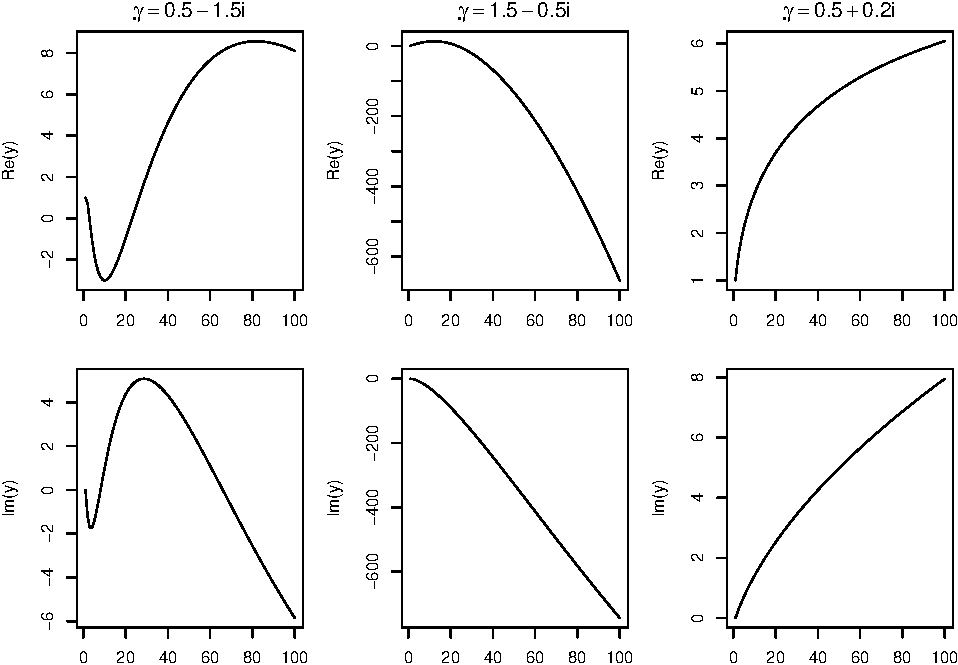
\includegraphics{Svetunkov---Svetunkov---Complex-Valued-Econometrics_files/figure-latex/trendTrajectories-1.pdf}
\caption{\label{fig:trendTrajectories}Different trajectories of trend with different values of the parameter \(\underline{\gamma}\): 0.5-1.5i, 1.5-0.5i, and 0.5+0.2i.}
\end{figure}

As we can see, the non-linear transformation gives the cLR flexibility in capturing various types of trends in the data, making it a much more flexible instrument for modelling than the real-valued regressions. Furthermore, this flexibility in the trend can be used in the real-valued models as well, if we substitute all the complex variables and parameters (except for \(\underline{\gamma}\)) by their real-valued counterparts. The model will then produce a complex response variable, the imaginary part of which can be dropped.

To better understand how the cLR model with the trend works, we can represent it in the exponential form:
\begin{equation}
    t^{\underline{\gamma}} = \exp (\underline{\gamma} \ln t) = t^{\gamma_r} \exp (i \gamma_i \ln t),
    \label{eq:trendExp}
\end{equation}
where \(\underline{\gamma}=\gamma_r + i \gamma_i\). The form \eqref{eq:trendExp} shows that the real part of the parameter \(\underline{\gamma}\) controls the magnitude of the resulting complex variable, while the imaginary one controls how fast the argument (angle) changes. So, the more stable trajectories (closer to the linear ones) will be obtained with \(\gamma_i\) close to zero, while the speed of the change in the trajectory is regulated by \(\gamma_r\).

Another way to look at the complex-valued trend is to use the trigonometric form of complex variable:
\begin{equation}
    t^{\underline{\gamma}} = t^{\gamma_r} \left(\cos (\gamma_i \ln t) + i \sin (\gamma_i \ln t) \right) .
    \label{eq:trendTrig}
\end{equation}
This form tells us that fundamentally any trajectory from the complex-valued trend is trigonometric, but \(\gamma_i\) regulates the strength of the cosine/sine waves for the respective real and imaginary parts of the complex response variable.

\hypertarget{example-in-r}{%
\subsection{Example in R}\label{example-in-r}}

In R, the trend is supported in the \texttt{clm()} function from the \texttt{complex} package via the formula. Here is an example:

\begin{Shaded}
\begin{Highlighting}[]
\CommentTok{\# Set random seed for reproducibility}
\KeywordTok{set.seed}\NormalTok{(}\DecValTok{41}\NormalTok{)}
\CommentTok{\# Sample size}
\NormalTok{obs \textless{}{-}}\StringTok{ }\DecValTok{100}
\CommentTok{\# Create an explanatory variable}
\NormalTok{x \textless{}{-}}\StringTok{ }\KeywordTok{complex}\NormalTok{(}\DataTypeTok{real=}\KeywordTok{rnorm}\NormalTok{(obs,}\DecValTok{100}\NormalTok{,}\DecValTok{10}\NormalTok{), }\DataTypeTok{imaginary=}\KeywordTok{rnorm}\NormalTok{(obs,}\DecValTok{50}\NormalTok{,}\DecValTok{5}\NormalTok{))}
\CommentTok{\# Generate parameters}
\NormalTok{b0 \textless{}{-}}\StringTok{ }\DecValTok{2} \OperatorTok{+}\StringTok{ }\FloatTok{1.5}\NormalTok{i}
\NormalTok{b1 \textless{}{-}}\StringTok{ }\FloatTok{0.8} \OperatorTok{{-}}\StringTok{ }\FloatTok{0.4}\NormalTok{i}
\NormalTok{b2 \textless{}{-}}\StringTok{ }\FloatTok{0.5} \OperatorTok{+}\StringTok{ }\FloatTok{0.2}\NormalTok{i}
\CommentTok{\# Generate error term from the complex normal distribution}
\NormalTok{e \textless{}{-}}\StringTok{ }\KeywordTok{rcnorm}\NormalTok{(obs, }\DecValTok{0}\NormalTok{, }\DataTypeTok{sigma2=}\FloatTok{0.25}\NormalTok{, }\DataTypeTok{varsigma2=}\FloatTok{0.16+0.09}\NormalTok{i)}
\CommentTok{\# Generate the data using non{-}linear model}
\NormalTok{y \textless{}{-}}\StringTok{ }\KeywordTok{exp}\NormalTok{(b0 }\OperatorTok{+}\StringTok{ }\NormalTok{b1 }\OperatorTok{*}\StringTok{ }\KeywordTok{log}\NormalTok{(x) }\OperatorTok{+}\StringTok{ }\NormalTok{b2 }\OperatorTok{*}\StringTok{ }\KeywordTok{log}\NormalTok{(}\KeywordTok{c}\NormalTok{(}\DecValTok{1}\OperatorTok{:}\NormalTok{obs)) }\OperatorTok{+}\StringTok{ }\NormalTok{e)}
\CommentTok{\# Merge it to the matrix}
\NormalTok{complexData \textless{}{-}}\StringTok{ }\KeywordTok{data.frame}\NormalTok{(}\DataTypeTok{y=}\NormalTok{y,}\DataTypeTok{x=}\NormalTok{x)}
\end{Highlighting}
\end{Shaded}

The code above will generate data with a slowly increasing trend (similar to the one shown in Figure \ref{fig:trendTrajectories}), which is shown in Figure \ref{fig:dataWithTrend}

\begin{figure}
\centering
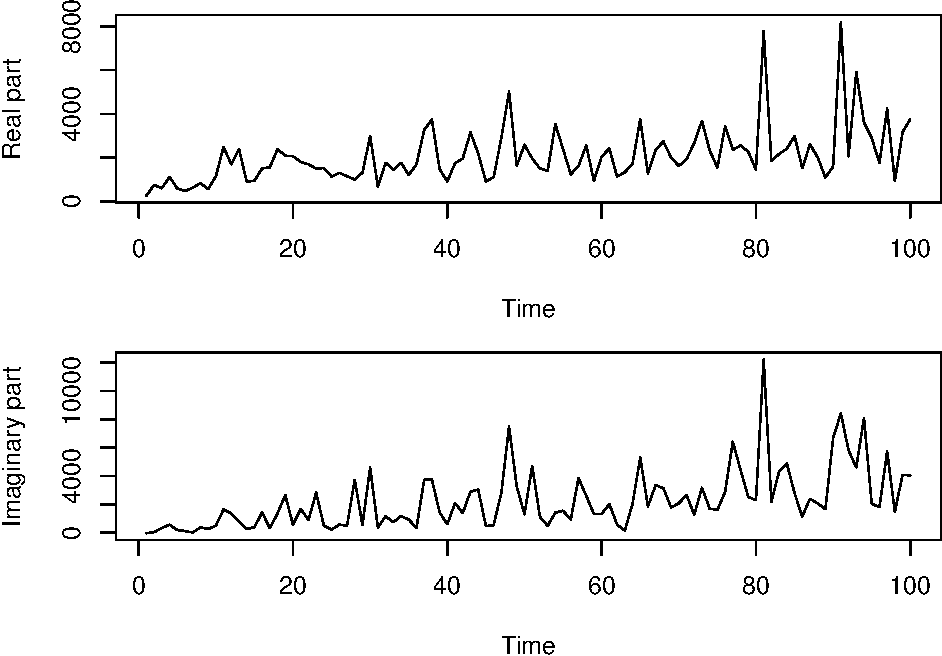
\includegraphics{Svetunkov---Svetunkov---Complex-Valued-Econometrics_files/figure-latex/dataWithTrend-1.pdf}
\caption{\label{fig:dataWithTrend}Generated time series with a trend.}
\end{figure}

Applying a complex linear regression to the data with the same formula as in the DGP gives us the following estimates of parameters:

\begin{Shaded}
\begin{Highlighting}[]
\CommentTok{\# Apply a model with the trend in logarithms}
\NormalTok{clrModel \textless{}{-}}\StringTok{ }\KeywordTok{clm}\NormalTok{(}\KeywordTok{log}\NormalTok{(y)}\OperatorTok{\textasciitilde{}}\KeywordTok{log}\NormalTok{(x)}\OperatorTok{+}\KeywordTok{log}\NormalTok{(trend), complexData, }\DataTypeTok{subset=}\DecValTok{1}\OperatorTok{:}\DecValTok{80}\NormalTok{)}
\KeywordTok{summary}\NormalTok{(clrModel)}
\end{Highlighting}
\end{Shaded}

\begin{verbatim}
## Complex Linear Regression estimated via clm()
## Response variable: logy
## Loss function used in estimation: likelihood
## Coefficients:
##               Estimate Std. Error Lower 2.5% Upper 97.5%  
## (Intercept)_r   3.8248     2.7186    -1.5904      9.2400  
## (Intercept)_i   5.6307     1.3591     2.9235      8.3380 *
## log(x)_r        0.3237     0.5685    -0.8087      1.4561  
## log(x)_i       -1.2205     0.2842    -1.7867     -0.6544 *
## log(trend)_r    0.5124     0.0604     0.3921      0.6327 *
## log(trend)_i    0.1836     0.0302     0.1235      0.2437 *
## 
## Error covariance matrix:
##        e_r    e_i
## e_r 0.2416 0.0735
## e_i 0.0735 0.0604
## 
## Sample size: 80
## Number of estimated parameters: 4.5
## Number of degrees of freedom: 75.5
## Information criteria:
##     AIC    AICc     BIC    BICc 
## 78.6004 79.2649 89.3195 90.7753
\end{verbatim}

The resulting model fit and the forecast for the next 20 observations are shown in Figure \ref{fig:dataWithTrendForecast}:

\begin{Shaded}
\begin{Highlighting}[]
\CommentTok{\# Extract fitted values and transform to the original scale}
\KeywordTok{fitted}\NormalTok{(clrModel) }\OperatorTok{|}\ErrorTok{\textgreater{}}\StringTok{ }\KeywordTok{exp}\NormalTok{() {-}\textgreater{}}\StringTok{ }\NormalTok{yFitted}
\NormalTok{yForecast \textless{}{-}}\StringTok{ }\KeywordTok{predict}\NormalTok{(clrModel, }\DataTypeTok{newdata=}\KeywordTok{tail}\NormalTok{(complexData, }\DecValTok{20}\NormalTok{))}

\CommentTok{\# Setup the canvas}
\KeywordTok{par}\NormalTok{(}\DataTypeTok{mfcol=}\KeywordTok{c}\NormalTok{(}\DecValTok{2}\NormalTok{,}\DecValTok{1}\NormalTok{), }\DataTypeTok{mar=}\KeywordTok{c}\NormalTok{(}\DecValTok{4}\NormalTok{,}\DecValTok{4}\NormalTok{,}\DecValTok{1}\NormalTok{,}\DecValTok{1}\NormalTok{))}
\CommentTok{\# Plot the real part}
\KeywordTok{plot}\NormalTok{(}\KeywordTok{Re}\NormalTok{(complexData}\OperatorTok{$}\NormalTok{y), }\DataTypeTok{type=}\StringTok{"l"}\NormalTok{,}
     \DataTypeTok{xlab=}\StringTok{"Time"}\NormalTok{, }\DataTypeTok{ylab=}\StringTok{"Real part"}\NormalTok{)}
\KeywordTok{lines}\NormalTok{(}\KeywordTok{Re}\NormalTok{(yFitted), }\DataTypeTok{col=}\StringTok{"purple"}\NormalTok{, }\DataTypeTok{lwd=}\DecValTok{2}\NormalTok{, }\DataTypeTok{lty=}\DecValTok{2}\NormalTok{)}
\KeywordTok{exp}\NormalTok{(yForecast}\OperatorTok{$}\NormalTok{mean) }\OperatorTok{|}\ErrorTok{\textgreater{}}\StringTok{ }\KeywordTok{Re}\NormalTok{() }\OperatorTok{|}\ErrorTok{\textgreater{}}
\StringTok{    }\KeywordTok{lines}\NormalTok{(}\DataTypeTok{x=}\KeywordTok{c}\NormalTok{(}\DecValTok{81}\OperatorTok{:}\DecValTok{100}\NormalTok{), }\DataTypeTok{col=}\StringTok{"blue"}\NormalTok{, }\DataTypeTok{lwd=}\DecValTok{2}\NormalTok{, }\DataTypeTok{lty=}\DecValTok{2}\NormalTok{)}

\CommentTok{\# Plot the imaginary part}
\KeywordTok{plot}\NormalTok{(}\KeywordTok{Im}\NormalTok{(complexData}\OperatorTok{$}\NormalTok{y), }\DataTypeTok{type=}\StringTok{"l"}\NormalTok{,}
     \DataTypeTok{xlab=}\StringTok{"Time"}\NormalTok{, }\DataTypeTok{ylab=}\StringTok{"Imaginary part"}\NormalTok{)}
\KeywordTok{lines}\NormalTok{(}\KeywordTok{Im}\NormalTok{(yFitted), }\DataTypeTok{col=}\StringTok{"purple"}\NormalTok{, }\DataTypeTok{lwd=}\DecValTok{2}\NormalTok{, }\DataTypeTok{lty=}\DecValTok{2}\NormalTok{)}
\KeywordTok{exp}\NormalTok{(yForecast}\OperatorTok{$}\NormalTok{mean) }\OperatorTok{|}\ErrorTok{\textgreater{}}\StringTok{ }\KeywordTok{Im}\NormalTok{() }\OperatorTok{|}\ErrorTok{\textgreater{}}
\StringTok{    }\KeywordTok{lines}\NormalTok{(}\DataTypeTok{x=}\KeywordTok{c}\NormalTok{(}\DecValTok{81}\OperatorTok{:}\DecValTok{100}\NormalTok{), }\DataTypeTok{col=}\StringTok{"blue"}\NormalTok{, }\DataTypeTok{lwd=}\DecValTok{2}\NormalTok{, }\DataTypeTok{lty=}\DecValTok{2}\NormalTok{)}
\end{Highlighting}
\end{Shaded}

\begin{figure}
\centering
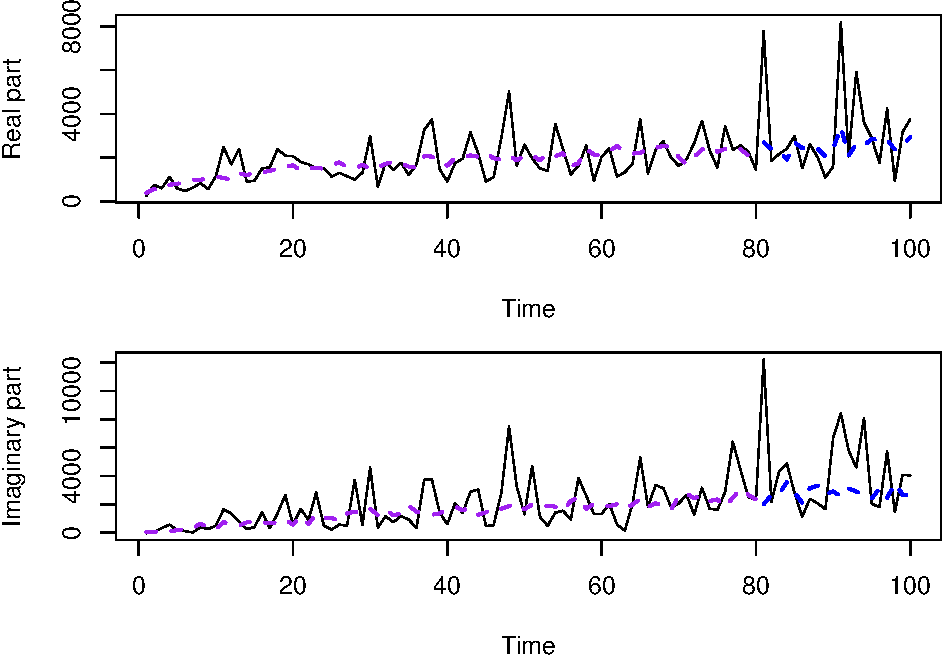
\includegraphics{Svetunkov---Svetunkov---Complex-Valued-Econometrics_files/figure-latex/dataWithTrendForecast-1.pdf}
\caption{\label{fig:dataWithTrendForecast}cLR applied to the generated data with a trend.}
\end{figure}

As we can see, this example shows how a non-linear trend can be estimated and then used for forecasting using a complex linear regression model.

\hypertarget{complex-ar}{%
\section{Complex AR}\label{complex-ar}}

One of the possible ways of modelling dynamics is by saying that future values of the variable depend on its past ones. \citet{Box1976}, who have developed a theory and methodology of so called ``AutoRegressive Integrated Moving Average'' (or ARIMA), provide an example of a series of CO\(_2\) output by a furnace with variable gas rate. In that situation the future amount of carbon dioxide will depend on the amount the furnace produced on the previous observations. This is one of example of an AR process. An interested reader is directed to Chapter 8 of \citet{SvetunkovAdam}, where the ARIMA model is discussed in more detail.

Mathematically the cAR model can be represented in a vector form, which will make it look more similar to vector AR rather than to the univariate one. However, the cAR model is restricted with just two time series and thus can be represented using complex variables:
\begin{equation}
    \underline{y}_t = \underline{\beta}_0 + \underline{\phi}_1 \underline{y}_{t-1} + \dots + \underline{\phi}_p \underline{y}_{t-p} + \underline{\epsilon}_t ,
    \label{eq:ComplexAR}
\end{equation}
where \(\phi_j\) is the \(j\)-th parameter, and \(p\) is the order of the model, complex autoregression, cAR(p). The same model can be rewritten in the conventional polynomial form using a backshift operator \(B\):
\begin{equation}
    \left(1 - \underline{\phi}_1 B - \dots - \underline{\phi}_p B^p \right) \underline{y}_t  = \underline{\beta}_0 + \underline{\epsilon}_t .
    \label{eq:ComplexARPolynomial}
\end{equation}
This form is convenient for what follows, e.g.~for the discussion of unit roots calculation. But also, if we add the already discussed static elements to the right-hand side of \eqref{eq:ComplexAR} or \eqref{eq:ComplexARPolynomial}, namely \(\underline{\beta}_1 \underline{x}_{1,t} + \dots + \underline{\beta}_{k-1} \underline{x}_{k-1,t}\), then the model will transform into cARX(p), combining the properties of the cLR and cAR.

Similarly to the conventional AR, it can be shown how complex ACF/PACF (discussed in Subsection \ref{assumptionsResidualsAuto}) behave for different orders of cAR. In this monograph, for simplicity, we only provide an example of cAR(1) without an intercept, noting that the logic for the higher orders is similar \citep[ has similar derivations for the real-valued AR(p) in Section 8.3]{SvetunkovAdam}.

The cAR(1) model is defined as:
\begin{equation}
    \underline{y}_t = \underline{\phi}_1 \underline{y}_{t-1} + \underline{\epsilon}_t .
    \label{eq:ComplexAR1Step1}
\end{equation}
The covariance between the most recent and the previous observations can then be calculated as (note here that we provide the formula for the conjugate covariance, but the calculations for the direct one will be similar):
\begin{equation}
    \mathrm{cov} \left(\underline{y}_t, \underline{y}_{t-1} \right) = \mathrm{cov} \left(\underline{\phi}_1 \underline{y}_{t-1} + \underline{\epsilon}_t, \underline{y}_{t-1} \right) ,
    \label{eq:ComplexAR1Step2}
\end{equation}
which given the basic assumptions of models (Section \ref{assumptionsResiduals}) equals to:
\begin{equation}
    \mathrm{cov} \left(\underline{y}_t, \underline{y}_{t-1} \right) = \underline{\phi}_1 \mathrm{cov} \left( \underline{y}_{t-1}, \underline{y}_{t-1} \right) .
    \label{eq:ComplexAR1Step3}
\end{equation}
Now, depending on the type of covariance we need, we get:

\begin{enumerate}
\def\labelenumi{\arabic{enumi}.}
\tightlist
\item
  For the conjugate one:
  \begin{equation}
   \mathrm{cov}\left(\underline{y}_t, \underline{y}_{t-1} \right) = \underline{\phi}_1 \sigma^2_{y_t} ;
   \label{eq:ComplexAR1ConjCov}
  \end{equation}
\item
  For the direct one:
  \begin{equation}
   cov \left(\underline{y}_t, \underline{y}_{t-1} \right) = \underline{\phi}_1 \varsigma^2_{y_t} .
   \label{eq:ComplexAR1DirCov}
  \end{equation}
\end{enumerate}

If we now insert \eqref{eq:ComplexAR1ConjCov} and \eqref{eq:ComplexAR1DirCov} into the respective formulae for the conjugate and direct correlations (Section \ref{correlationTypes}, equations \eqref{eq:correlationConjugate} and \eqref{eq:correlationDirect}), we will get the values of the cACF for the first lag according to:

\begin{enumerate}
\def\labelenumi{\arabic{enumi}.}
\item
  Conjugate correlation:
  \begin{equation}
   \rho(1) = \frac{\sqrt{\underline{\phi}_1 \sigma^2_{y_t} \underline{\phi}_1 \sigma^2_{y_t}}}{\sigma_{y_t}^2} = | \underline{\phi}_1 |;
   \label{eq:ComplexAR1ConjCor}
  \end{equation}
\item
  Direct correlation:
  \begin{equation}
   \varrho(1) = \frac{\underline{\phi}_1 \varsigma^2_{y_t}}{\varsigma^2_{y_t}} = \underline{\phi}_1.
   \label{eq:ComplexAR1DirCor}
  \end{equation}
\end{enumerate}

As we can see from the formula \eqref{eq:ComplexAR1ConjCor}, the specific value of the cAR(1) parameter is lost because of the geometric mean in the formula: we end up with a magnitude of the complex variable instead of it real and imaginary parts. On the other hand, the direct cACF \eqref{eq:ComplexAR1DirCor} keeps the information about the cAR(1) parameter. However, the two formulae above are calculated in terms of expectations and their sample estimates might be slightly different. Specifically, the direct correlation \eqref{eq:ComplexAR1DirCor} relies on the sample estimate of the direct variance of the response variable \(y_t\), which might become equal to zero if the variances of the real and the imaginary parts of the complex variable are similar (as discussed in Section \ref{correlationDirect}). This means that in some situations the values of the direct cACF might become greater than one, leading to potential losses in information. But this also means that both conjugate and direct cACFs should be used for the analysis of complex time series: each of them has issues, but both of them give much clearer information about the potential process.

If we calculate the covariance for the cAR(1) between the values \(y_{t}\) and \(y_{t-2}\), we will get the following (the reader is encouraged to do the calculations manually to check the correctness of the final result):

\begin{enumerate}
\def\labelenumi{\arabic{enumi}.}
\item
  Conjugate correlation:
  \begin{equation}
   \rho(2) = | \underline{\phi}_1^2 |;
   \label{eq:ComplexAR1ConjCor}
  \end{equation}
\item
  Direct correlation:
  \begin{equation}
   \varrho(2) =  \underline{\phi}_1^2.
   \label{eq:ComplexAR1DirCor}
  \end{equation}
\end{enumerate}

In principles, it can be shown that the main properties of real-valued AR discussed by \citet{Box1976} hold widely for the cAR processes: cACF will decline exponentially starting from the lag p.~Note however that the direct cACF involves the power of a complex number, which means that in some situations, for some values of the complex parameter \(\underline{\phi}_1\), the cACF will decline harmonically rather than exponentially.

The more useful (at least potentially) property for cAR(p) is the behaviour of the cPACF. This function shows the relations between specific lags without the effect of all the interim lags, i.e.~cleaned from the autocorrelations between the neighbouring lags. One of ways of calculating the cPACF for a lag \(\tau\) is to estimate the following model:
\begin{equation}
    \underline{y}_t = \underline{\phi}_1 \underline{y}_{t-1} + \dots + \underline{\phi}_\tau \underline{y}_{t-\tau} + \underline{\epsilon}_t
    \label{eq:cPACFModel}
\end{equation}
and getting the coefficient \(\underline{\phi}_\tau\). Repeating this procedure for all lags of interest, we get a cPACF. The model \eqref{eq:cPACFModel} can be estimated using OLS or CLS, which will result in respective conjugate and direct cPACF.

It can be shown that for the cAR(p) process, both conjugate and direct cPACF will drop to zero abruptly after the lag p and that both of them will produce complex numbers, reflecting the respective parts of the coefficients of the cAR(p) model. However, the direct cPACF might have issues similar to the ones the direct cACF has if the variances of the real and the imaginary parts of the response variable are close to each other.

As we see, the complex AR(p) has similar properties to the real-valued one, but it should be analysed using both conjugate and direct cACF/cPACF.

Finally, in Box-Jenkins methodology, it is important for the AR(p) processes to be stationary, otherwise they become explosive and cannot be efficiently identified at the model building stage. The stationarity condition for AR(p) in \citet{Box1976} is that the roots of the polynomial formed from the parameters of the AR model should all lie outside the unit circle. For AR(1) this simplifies to \(|\phi_1|<1\). The same conditions hold for the cAR(p) processes, meaning that the magnitudes of the complex parameters are considered. For the cAR(1), the stationarity condition is \(|\underline{\phi}_1|<1\). But more widely, for cAR(p), it is that the roots of the following polynomial:
\begin{equation}
    1 - \underline{\phi}_1 x - \underline{\phi}_2 x^2 - \dots - \underline{\phi}_p x^p = 0
    \label{eq:ComplexARPolyRoots}
\end{equation}
should all lie outside the unit circle (be greater than one by absolute value).

\hypertarget{example-in-r-1}{%
\subsection{Example in R}\label{example-in-r-1}}

For demonstration purposes we consider the cAR(1) process to see how cACF/cPACF and the data will look

\begin{Shaded}
\begin{Highlighting}[]
\CommentTok{\# Sample size}
\KeywordTok{set.seed}\NormalTok{(}\DecValTok{41}\NormalTok{)}
\CommentTok{\# Number of observations}
\NormalTok{obs \textless{}{-}}\StringTok{ }\DecValTok{110}
\CommentTok{\# Parameters}
\NormalTok{b0 \textless{}{-}}\StringTok{ }\DecValTok{100}\OperatorTok{+}\NormalTok{50i}
\NormalTok{phi1 \textless{}{-}}\StringTok{ }\FloatTok{0.5} \OperatorTok{+}\StringTok{ }\FloatTok{0.2}\NormalTok{i}
\CommentTok{\# Complex white noise}
\NormalTok{e \textless{}{-}}\StringTok{ }\KeywordTok{rcnorm}\NormalTok{(obs, }\DecValTok{0}\NormalTok{, }\DataTypeTok{sigma2=}\DecValTok{25}\NormalTok{, }\DataTypeTok{varsigma2=}\DecValTok{16}\OperatorTok{+}\NormalTok{9i)}
\NormalTok{y \textless{}{-}}\StringTok{ }\KeywordTok{vector}\NormalTok{(}\StringTok{"complex"}\NormalTok{, obs)}
\CommentTok{\# Initial value}
\NormalTok{y[}\DecValTok{1}\NormalTok{] \textless{}{-}}\StringTok{ }\NormalTok{b0 }\OperatorTok{+}\StringTok{ }\NormalTok{e[}\DecValTok{1}\NormalTok{]}
\CommentTok{\# The cAR(1)}
\ControlFlowTok{for}\NormalTok{(i }\ControlFlowTok{in} \DecValTok{2}\OperatorTok{:}\NormalTok{obs)\{}
\NormalTok{    y[i] \textless{}{-}}\StringTok{ }\NormalTok{phi1 }\OperatorTok{*}\StringTok{ }\NormalTok{y[i}\DecValTok{{-}1}\NormalTok{] }\OperatorTok{+}\StringTok{ }\NormalTok{b0 }\OperatorTok{+}\StringTok{ }\NormalTok{e[i]}
\NormalTok{\}}
\CommentTok{\# Drop the first 10 observations as a burn{-}in period}
\NormalTok{y \textless{}{-}}\StringTok{ }\NormalTok{y[}\OperatorTok{{-}}\KeywordTok{c}\NormalTok{(}\DecValTok{1}\OperatorTok{:}\DecValTok{10}\NormalTok{)]}
\end{Highlighting}
\end{Shaded}

The conjugate cACF/cPACF are shown in Figures \ref{fig:complexAR1cACF} and \ref{fig:complexAR1cPACF}:

\begin{Shaded}
\begin{Highlighting}[]
\KeywordTok{cacf}\NormalTok{(y, }\DataTypeTok{method=}\StringTok{"conjugate"}\NormalTok{, }\DataTypeTok{main=}\StringTok{""}\NormalTok{)}
\end{Highlighting}
\end{Shaded}

\begin{figure}
\centering
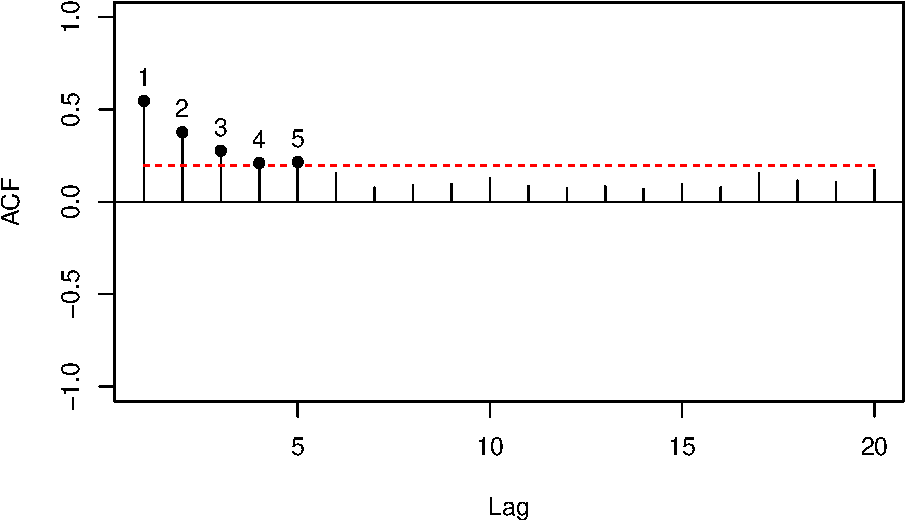
\includegraphics{Svetunkov---Svetunkov---Complex-Valued-Econometrics_files/figure-latex/complexAR1cACF-1.pdf}
\caption{\label{fig:complexAR1cACF}Conjugate cACF of the complex AR(1).}
\end{figure}

As we see from Figure \ref{fig:complexAR1cACF}, the cACF declines after the lag 1. Notably, the cACF for lag one equals to 0.546, which is close to the true value of the magnitude of the parameter \(\phi_1=0.5+0.2i\) is 0.5385165.

\begin{Shaded}
\begin{Highlighting}[]
\KeywordTok{cpacf}\NormalTok{(y, }\DataTypeTok{method=}\StringTok{"conjugate"}\NormalTok{, }\DataTypeTok{main=}\StringTok{""}\NormalTok{)}
\end{Highlighting}
\end{Shaded}

\begin{figure}
\centering
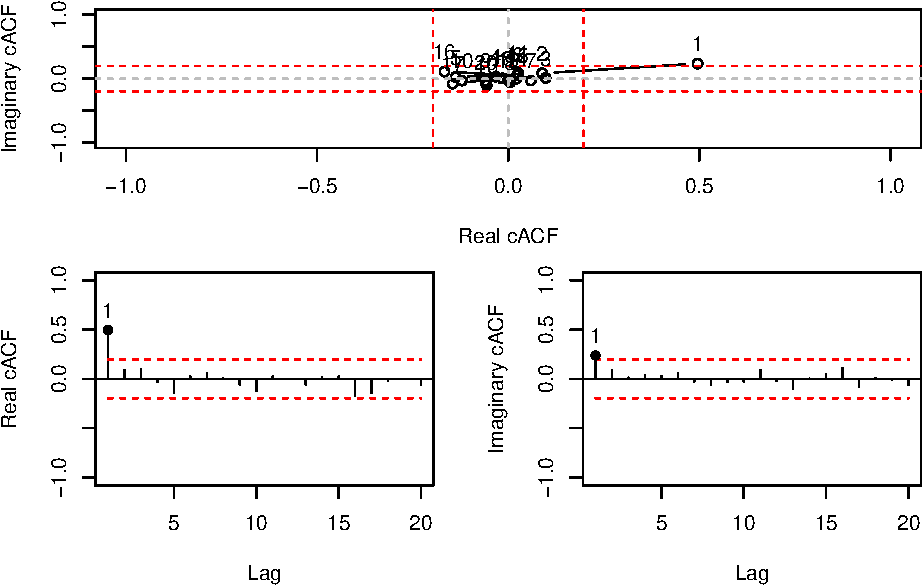
\includegraphics{Svetunkov---Svetunkov---Complex-Valued-Econometrics_files/figure-latex/complexAR1cPACF-1.pdf}
\caption{\label{fig:complexAR1cPACF}Conjugate cPACF of the complex AR(1).}
\end{figure}

The cPACF in Figure \ref{fig:complexAR1cPACF} demonstrates that both the real and the imaginary values drop to zero after the first observation, as expected for the AR(1) process. Notably, the value of the first cPACF is 0.495+0.236i, which is close to the true value of the parameter.

The direct cACF and cPACF are shown in Figures \ref{fig:complexAR1cACFDir} and \ref{fig:complexAR1cpACFDir}, roughly giving the same information as their conjugate counterparts. We should note however that the direct cACF has the more detailed information about the dynamic relations in the data than the conjugate one.
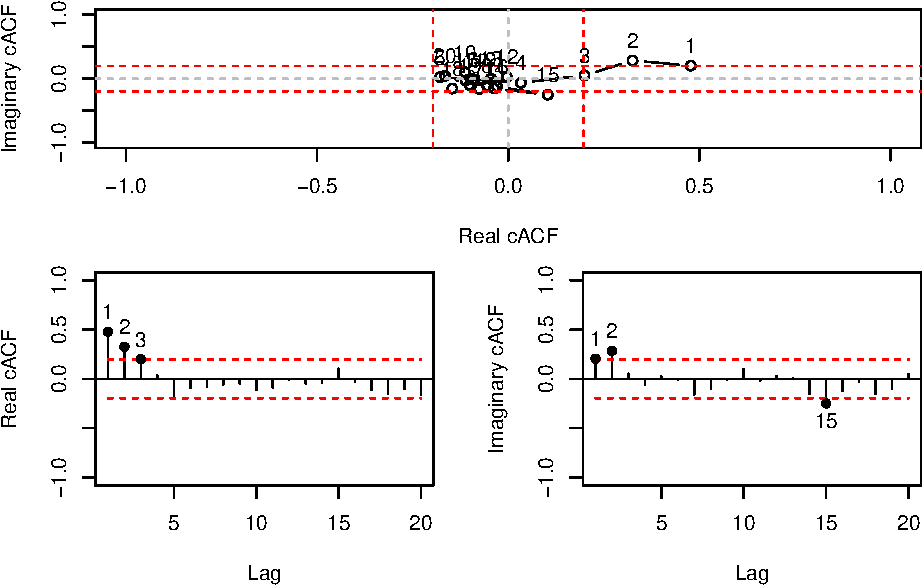
\includegraphics{Svetunkov---Svetunkov---Complex-Valued-Econometrics_files/figure-latex/complexAR1cACFDir-1.pdf}

Although, both plots contain values outside of the 95\% non-rejection region, these could be considered as happening at random and can be neglected.

\begin{figure}
\centering
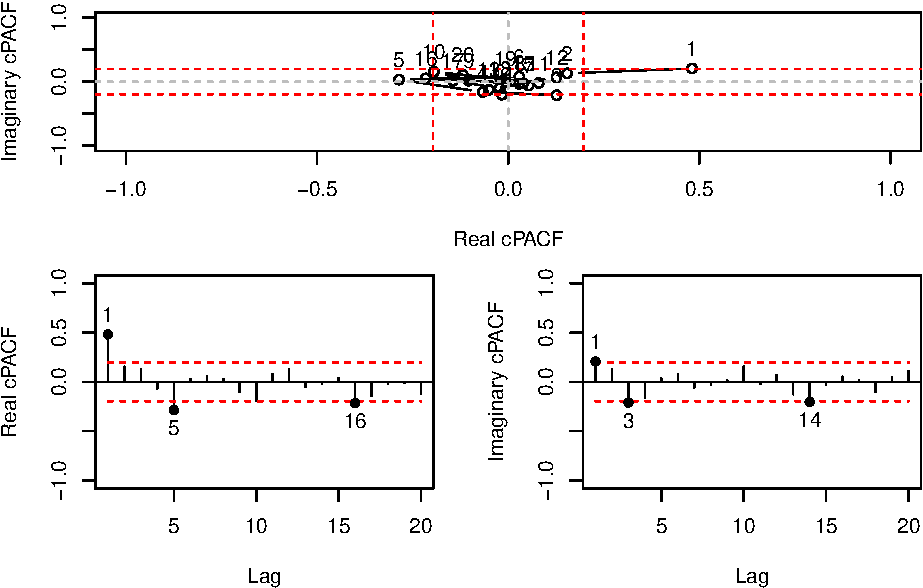
\includegraphics{Svetunkov---Svetunkov---Complex-Valued-Econometrics_files/figure-latex/complexAR1cpACFDir-1.pdf}
\caption{\label{fig:complexAR1cpACFDir}Direct cPACF of the complex AR(1).}
\end{figure}

It is worth noting that in both Figures \ref{fig:complexAR1cACFDir} and \ref{fig:complexAR1cpACFDir} the first values of the cACF/cPACF are close to the true value of \(0.5+0.2i\).

Finally, the plot in Figure \ref{fig:complexAR1Plot} shows the generated data on the complex plane and the dynamics of both the real and the imaginary parts.

\begin{figure}
\centering
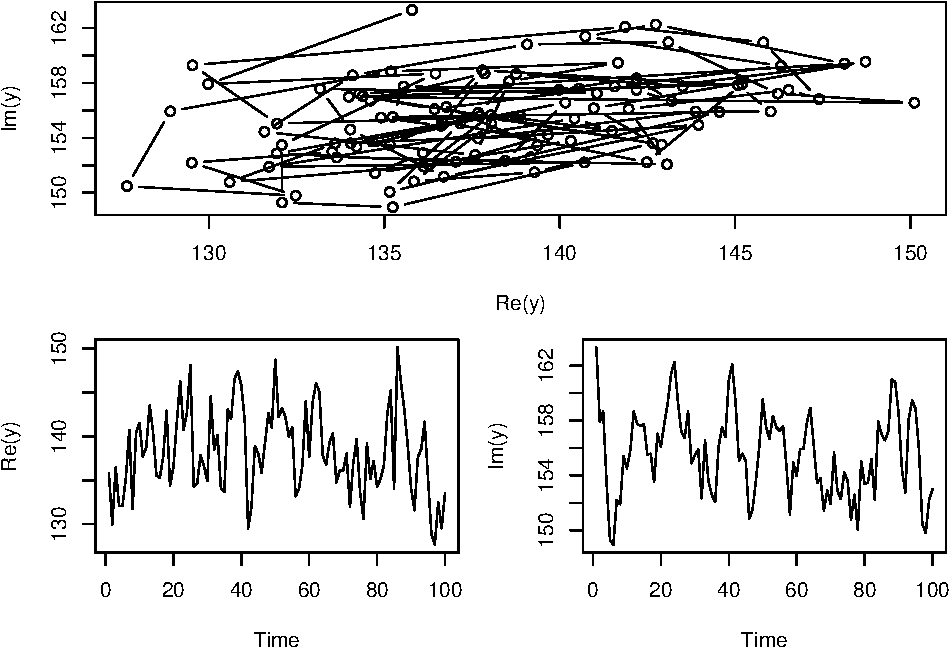
\includegraphics{Svetunkov---Svetunkov---Complex-Valued-Econometrics_files/figure-latex/complexAR1Plot-1.pdf}
\caption{\label{fig:complexAR1Plot}Visualisation of the cAR(1) process.}
\end{figure}

When it comes to applying a model and to forecasting, the same \texttt{clm()} function from the \texttt{complex} package in R can be used:

\begin{Shaded}
\begin{Highlighting}[]
\CommentTok{\# Fit the model with intercept and AR(1)}
\NormalTok{cAR1Model \textless{}{-}}\StringTok{ }\KeywordTok{clm}\NormalTok{(y}\OperatorTok{\textasciitilde{}}\DecValTok{1}\NormalTok{, }\DataTypeTok{orders=}\KeywordTok{c}\NormalTok{(}\DecValTok{1}\NormalTok{,}\DecValTok{0}\NormalTok{,}\DecValTok{0}\NormalTok{), }\DataTypeTok{subset=}\KeywordTok{c}\NormalTok{(}\DecValTok{1}\OperatorTok{:}\DecValTok{80}\NormalTok{))}
\CommentTok{\# Generate the summary}
\KeywordTok{summary}\NormalTok{(cAR1Model)}
\end{Highlighting}
\end{Shaded}

\begin{verbatim}
## cARIMA(1,0,0) estimated via clm()
## Response variable: y
## Loss function used in estimation: likelihood
## Coefficients:
##               Estimate Std. Error Lower 2.5% Upper 97.5%  
## (Intercept)_r 104.0038    17.8382    68.4797    139.5278 *
## (Intercept)_i  51.6885     9.1839    33.3991     69.9778 *
## yLag1_r         0.4825     0.0856     0.3122      0.6529 *
## yLag1_i         0.2075     0.0440     0.1198      0.2952 *
## 
## Error covariance matrix:
##         e_r    e_i
## e_r 17.4734 4.1781
## e_i  4.1781 4.6316
## 
## Sample size: 80
## Number of estimated parameters: 3.5
## Number of degrees of freedom: 76.5
## Information criteria:
##      AIC     AICc      BIC     BICc 
## 785.9517 786.3689 794.2888 795.2029
\end{verbatim}

The output above shows the estimates of parameters of the model, demonstrating that the OLS produced estimates close to the true values of parameters (as expected). After that we can generate forecast for the next 20 observations:

\begin{Shaded}
\begin{Highlighting}[]
\CommentTok{\# Dummy data. 20 rows tells the function what the horizon is}
\NormalTok{complexData20 \textless{}{-}}\StringTok{ }\KeywordTok{matrix}\NormalTok{(}\KeywordTok{rep}\NormalTok{(}\DecValTok{1}\NormalTok{,}\DecValTok{20}\NormalTok{),}\DecValTok{20}\NormalTok{,}\DecValTok{1}\NormalTok{)}
\CommentTok{\# Produce forecasts for the next 20 steps}
\NormalTok{yForecast \textless{}{-}}\StringTok{ }\KeywordTok{predict}\NormalTok{(cAR1Model, }\DataTypeTok{newdata=}\NormalTok{complexData20)}
\end{Highlighting}
\end{Shaded}

The only catch in the code above is to create a dummy \texttt{newdata} with the number of rows equal to the forecast horizon. This is a fix, needed because the \texttt{clm()} function focuses on explanatory variables. The forecasts from the function are shown in Figure \ref{fig:complexAR1Forecast}.

\begin{Shaded}
\begin{Highlighting}[]
\CommentTok{\# Produce the plot of the data and the forecasts}
\KeywordTok{par}\NormalTok{(}\DataTypeTok{mfcol=}\KeywordTok{c}\NormalTok{(}\DecValTok{2}\NormalTok{,}\DecValTok{1}\NormalTok{),}\DataTypeTok{mar=}\KeywordTok{c}\NormalTok{(}\DecValTok{4}\NormalTok{,}\DecValTok{4}\NormalTok{,}\DecValTok{1}\NormalTok{,}\DecValTok{1}\NormalTok{))}
\KeywordTok{plot}\NormalTok{(yForecast)}
\end{Highlighting}
\end{Shaded}

\begin{figure}
\centering
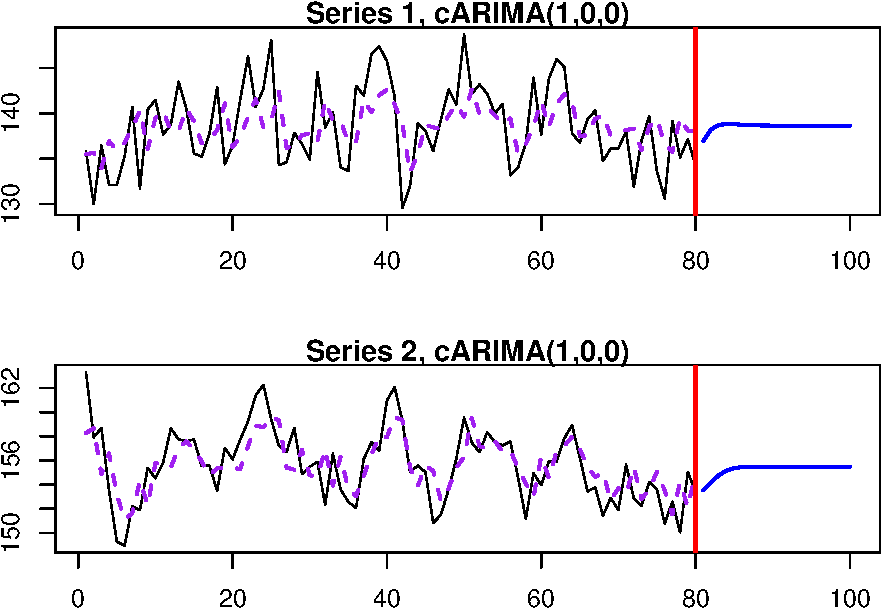
\includegraphics{Svetunkov---Svetunkov---Complex-Valued-Econometrics_files/figure-latex/complexAR1Forecast-1.pdf}
\caption{\label{fig:complexAR1Forecast}Forecasts for the cAR(1) process.}
\end{figure}

As we can see, the forecast trajectory from the cAR(1) model corresponds to the dampening line, which is a behaviour similar to the conventional real-valued AR(1) model \citep[e.g.~discussed in Subsection 8.1.1 of][]{SvetunkovAdam}.

\hypertarget{complex-ma}{%
\section{Complex MA}\label{complex-ma}}

Another type of the dynamic model discussed by \citet{Box1976}, is called ``Moving Average''. In case of complex variables, it can be formulated as:
\begin{equation}
    \underline{y}_t = \underline{\beta}_0 + \underline{\theta}_1 \underline{\epsilon}_{t-1} + \dots + \underline{\theta}_q \underline{\epsilon}_{t-q} + \underline{\epsilon}_t ,
    \label{eq:ComplexMA}
\end{equation}
where \(\theta_j\) is the \(j\)-th parameter, and \(q\) is the order of the model complex MA(q) model. Similar to the cAR, it can be written via polynomials:
\begin{equation}
    \underline{y}_t  = \underline{\beta}_0 + \left(1 + \underline{\theta}_1 B + \dots + \underline{\theta}_q B^q \right) \underline{\epsilon}_t .
    \label{eq:ComplexMAPolynomial}
\end{equation}
The idea of this model is that the new actual observation is formed as a linear combination of the past white noise. \citet{Box1976} continue the example with a CO\(_2\) output, showing that some random disturbances in the system in the past can impact the volume of the carbon dioxide at the current moment.

Using similar logic as in case of cAR, we will show how cACF and cPACF behave for cMA(1) without intercept, and then we will generalise their behaviour for cMA(q).

The cMA(1) model can be defined as:
\begin{equation}
    \underline{y}_t = \underline{\theta}_1 \underline{\epsilon}_{t-1} + \underline{\epsilon}_t .
    \label{eq:ComplexMA1}
\end{equation}
For the cACF, we need to calculate the covariance between the values on observations \(t\) and \(t-1\). Again, the formulae for the conjugate and the direct covariances will be similar at this stage:
\begin{equation}
    \mathrm{cov} \left(\underline{y}_t, \underline{y}_{t-1} \right) = \mathrm{cov}\left( \underline{\theta}_1 \underline{\epsilon}_{t-1} + \underline{\epsilon}_t, \underline{\theta}_1 \underline{\epsilon}_{t-2} + \underline{\epsilon}_{t-1} \right).
    \label{eq:ComplexMA1Step1}
\end{equation}
Given that the basic assumptions discussed in Chapter \ref{assumptions} hold for the ``true model'', the covariance is simplified to:
\begin{equation}
    \mathrm{cov} \left(\underline{y}_t, \underline{y}_{t-1} \right) = \underline{\theta}_1 \mathrm{cov}\left( \underline{\epsilon}_{t-1}, \underline{\epsilon}_{t-1} \right).
    \label{eq:ComplexMA1Step2}
\end{equation}

Based on this, the conjugate and the direct covariances will be equal to respectively:
\begin{equation}
    \mathrm{cov} \left(\underline{y}_t, \underline{y}_{t-1} \right) = \underline{\theta}_1 \sigma^2_{y_t}.
    \label{eq:ComplexMA1ConjCov}
\end{equation}
and
\begin{equation}
    {cov} \left(\underline{y}_t, \underline{y}_{t-1} \right) = \underline{\theta}_1 \varsigma^2_{y_t}.
    \label{eq:ComplexMA1DirCov}
\end{equation}
Note that in the formulae above, we use the fact that the variance of the error term will coincide with the variance of the response variable \(\underline{y}_t\), which becomes apparent from the original model formulation \eqref{eq:ComplexMA1}, assuming that the error term has a zero expectation. Inserting \eqref{eq:ComplexMA1ConjCov} and \eqref{eq:ComplexMA1DirCov} in the formulae for the conugate and direct correlations, we get that for the cMA(1), the first lag of the cACF equals to:

\begin{enumerate}
\def\labelenumi{\arabic{enumi}.}
\item
  Conjugate correlation:
  \begin{equation}
   \rho(1) = | \underline{\theta}_1 |;
   \label{eq:ComplexMA1ConjCor}
  \end{equation}
\item
  Direct correlation:
  \begin{equation}
   \varrho(1) =  \underline{\theta}_1.
   \label{eq:ComplexMA1DirCor}
  \end{equation}
\end{enumerate}

Similarly to how it was with the cAR(1) process, we see that the conjugate cACF is based on the magnitude of the complex parameter, while the direct one has the value itself in it. This comes with the same in-sample limitations as above with the direct correlation being sensitive to the similarity of the variances of the real and the imaginary parts of the response variable.

However, when it comes to the second lag of the cACF, the situation differs from the one with the cAR(1):
\begin{equation}
    \mathrm{cov} \left(\underline{y}_t, \underline{y}_{t-2} \right) = \mathrm{cov}\left( \underline{\theta}_1 \underline{\epsilon}_{t-1} + \underline{\epsilon}_t, \underline{\theta}_1 \underline{\epsilon}_{t-3} + \underline{\epsilon}_{t-2} \right) = 0 .
    \label{eq:ComplexMA1Lag2}
\end{equation}
This agrees with the behaviour of the cACF in case of the conventional real-valued MA(q) processes \citep{Box1976}: it falls to zero abruptly right after the lag q.

When it comes to the cPACF of cMA(1), its behaviour becomes similar to the behaviour of cACF for AR(1). This is because the model \eqref{eq:ComplexMA1} can be represented as an infinite cAR:
\begin{equation}
    \underline{y}_t = \sum_{j=1}^\infty -1^{j-1} \underline{\theta}_1^j \underline{y}_{t-j} + \underline{\epsilon}_t ,
    \label{eq:ComplexMA1Infinite}
\end{equation}
which is based on the fact that \(\underline{\epsilon}_t = \underline{y}_t - \underline{\theta}_1 \underline{\epsilon}_{t-1}\). In this situation, both conjugate and direct cPACF will decline either exponentially or harmonically, depending on the specific value of the complex parameter. In general, this ones again agrees with the behaviour of the conventional PACF in case of the real-valued MA(q) process.

As we see, the behaviour of both cACF and cPACF in case of cMA(q) model agrees with their behaviour in the real-valued model. Still, similarly to the cAR(p) process, both conjugate and direct cPACF should be used for time series analysis.

Continuing the similarities between the complex and the real-valued models, it can be shown that the property of the invertibility is easily transferable to the cMA(q) model from the conventional MA(q). The model will be invertible if all the roots of the following polynomial equation lie outside of the unit circle:
\begin{equation}
    1 + \underline{\theta}_1 x + \underline{\theta}_2 x^2 + \dots + \underline{\theta}_p x^p = 0 .
    \label{eq:ComplexMAPolyRoots}
\end{equation}

When it comes to estimating the model on a sample of data, we face several restrictions: the cMA part needs to be constructed recursively, because the new error from observation \(t\) is used on the next observations. This means that the analytical solutions according to OLS or CLS cannot be applied anymore, and we need to revert to the numeric optimisation. To that extent, CLS can no longer be used, because the standard solvers require the real-valued loss function, while the one from CLS is a complex one. So, when estimating cMA(q) model, we have to use either OLS or likelihood.

\hypertarget{example-in-r-2}{%
\subsection{Example in R}\label{example-in-r-2}}

Similarly to the cAR(p), we consider an R example, analysing how the cACF and cPACF behave in a special case of cMA(1) with an intercept:

\begin{Shaded}
\begin{Highlighting}[]
\CommentTok{\# Sample size}
\KeywordTok{set.seed}\NormalTok{(}\DecValTok{41}\NormalTok{)}
\CommentTok{\# Number of observations}
\NormalTok{obs \textless{}{-}}\StringTok{ }\DecValTok{110}
\CommentTok{\# Parameters}
\NormalTok{b0 \textless{}{-}}\StringTok{ }\DecValTok{100}\OperatorTok{+}\NormalTok{50i}
\NormalTok{theta1 \textless{}{-}}\StringTok{ }\FloatTok{{-}0.8} \OperatorTok{+}\StringTok{ }\FloatTok{0.2}\NormalTok{i}
\CommentTok{\# Complex white noise}
\NormalTok{e \textless{}{-}}\StringTok{ }\KeywordTok{rcnorm}\NormalTok{(obs, }\DecValTok{0}\NormalTok{, }\DataTypeTok{sigma2=}\DecValTok{25}\NormalTok{, }\DataTypeTok{varsigma2=}\DecValTok{16}\OperatorTok{+}\NormalTok{9i)}
\NormalTok{y \textless{}{-}}\StringTok{ }\KeywordTok{vector}\NormalTok{(}\StringTok{"complex"}\NormalTok{, obs)}
\CommentTok{\# Initial value}
\NormalTok{y[}\DecValTok{1}\NormalTok{] \textless{}{-}}\StringTok{ }\NormalTok{b0 }\OperatorTok{+}\StringTok{ }\NormalTok{e[}\DecValTok{1}\NormalTok{]}
\CommentTok{\# The cAR(1)}
\ControlFlowTok{for}\NormalTok{(i }\ControlFlowTok{in} \DecValTok{2}\OperatorTok{:}\NormalTok{obs)\{}
\NormalTok{    y[i] \textless{}{-}}\StringTok{ }\NormalTok{theta1 }\OperatorTok{*}\StringTok{ }\NormalTok{e[i}\DecValTok{{-}1}\NormalTok{] }\OperatorTok{+}\StringTok{ }\NormalTok{b0 }\OperatorTok{+}\StringTok{ }\NormalTok{e[i]}
\NormalTok{\}}
\CommentTok{\# Drop the first 10 observations as a burn{-}in period}
\NormalTok{y \textless{}{-}}\StringTok{ }\NormalTok{y[}\OperatorTok{{-}}\KeywordTok{c}\NormalTok{(}\DecValTok{1}\OperatorTok{:}\DecValTok{10}\NormalTok{)]}
\end{Highlighting}
\end{Shaded}

Because we use the same random seed value as before and the same value of the parameter as in case of cAR(1), we get time series, which look similar to the one generated from cAR(1) (see Figure \ref{fig:complexMA1Plot}, compared to Figure \ref{fig:complexAR1Plot}).

\begin{figure}
\centering
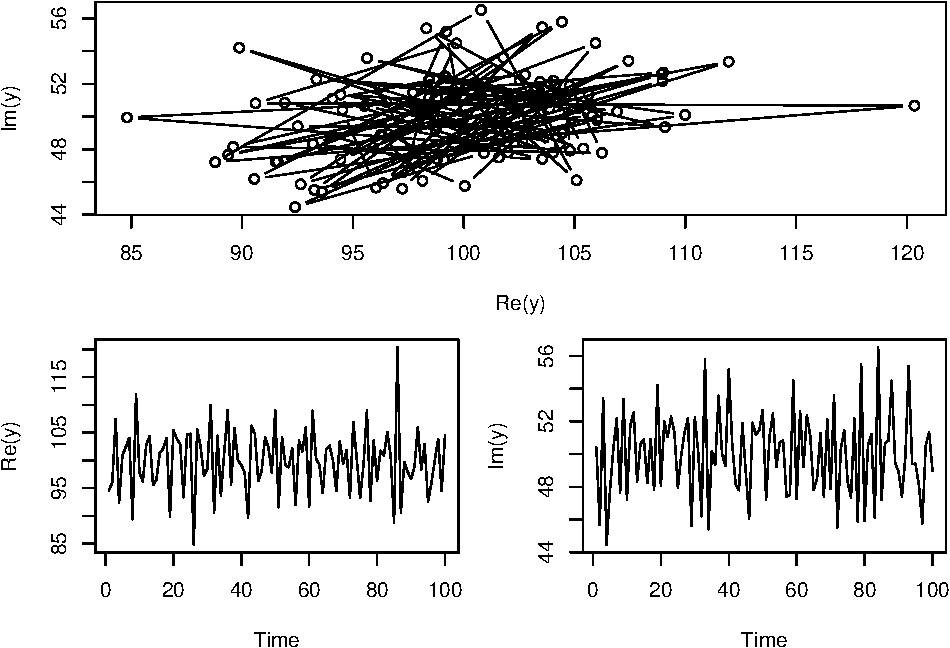
\includegraphics{Svetunkov---Svetunkov---Complex-Valued-Econometrics_files/figure-latex/complexMA1Plot-1.pdf}
\caption{\label{fig:complexMA1Plot}Visualisation of the cMA(1) process.}
\end{figure}

However, when we analyse cACF of the time series, we will spot an important difference - its values drop to zero abruptly right after the first lag.

\begin{Shaded}
\begin{Highlighting}[]
\KeywordTok{cacf}\NormalTok{(y, }\DataTypeTok{method=}\StringTok{"conjugate"}\NormalTok{, }\DataTypeTok{main=}\StringTok{""}\NormalTok{)}
\end{Highlighting}
\end{Shaded}

\begin{figure}
\centering
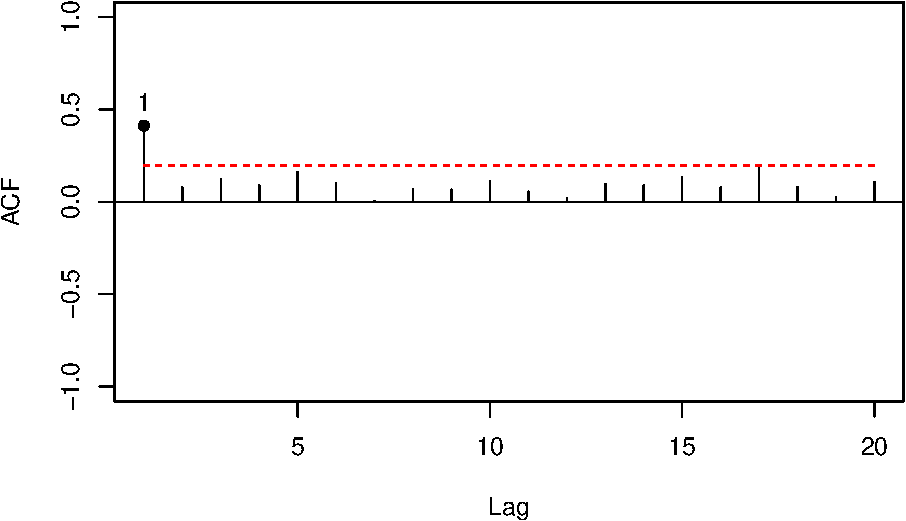
\includegraphics{Svetunkov---Svetunkov---Complex-Valued-Econometrics_files/figure-latex/complexMA1cACF-1.pdf}
\caption{\label{fig:complexMA1cACF}Conjugate cACF of the complex MA(1).}
\end{figure}

As we see from Figure \ref{fig:complexMA1cACF}, the only statistically significant lag (on 5\%) is the first one, all the others lie in the non-rejection region. We observe a similar behaviour in case of the direct cACF (Figure \ref{fig:complexMA1cACFDir}), although it is worth noting that the imaginary part of the direct cACF has all lags lying in the non-rejection region.

\begin{figure}
\centering
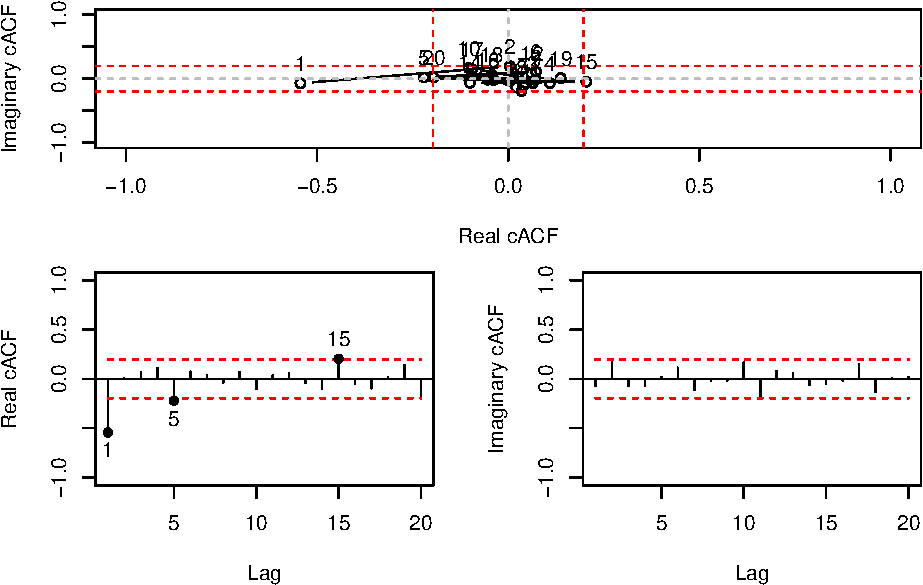
\includegraphics{Svetunkov---Svetunkov---Complex-Valued-Econometrics_files/figure-latex/complexMA1cACFDir-1.pdf}
\caption{\label{fig:complexMA1cACFDir}Direct cACF of the complex MA(1).}
\end{figure}

On the other hand, the conjugate and direct cPACF will decline exponentially, as discussed earlier. Figure \ref{fig:complexMA1cpACFDir} shows how the Direct cPACF looks for the complex MA(1), while Figure \ref{fig:complexMA1cPACF} shows the conjugate one. While the specific values are different for the two functions, they give roughly the same message: the cPACFs decline over time.

\begin{figure}
\centering
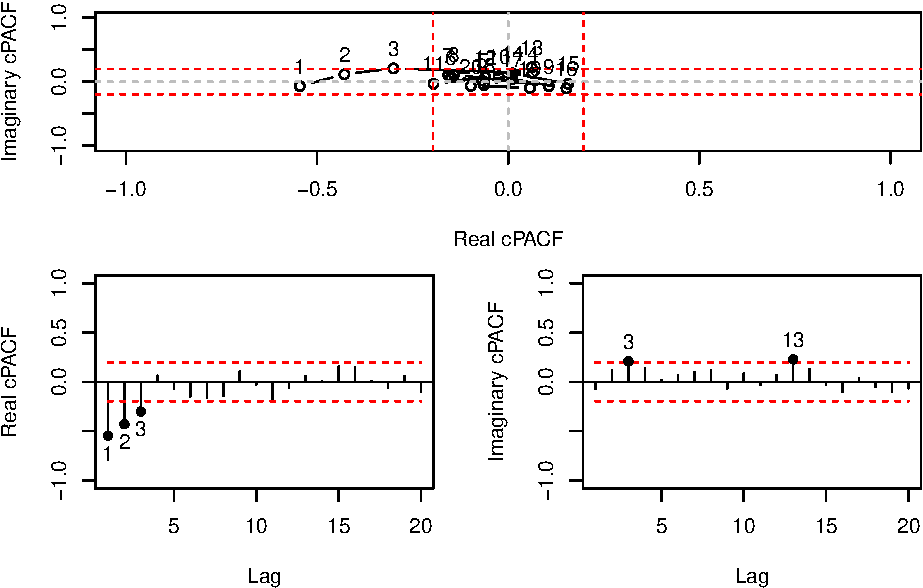
\includegraphics{Svetunkov---Svetunkov---Complex-Valued-Econometrics_files/figure-latex/complexMA1cpACFDir-1.pdf}
\caption{\label{fig:complexMA1cpACFDir}Direct cPACF of the complex MA(1).}
\end{figure}

\begin{Shaded}
\begin{Highlighting}[]
\KeywordTok{cpacf}\NormalTok{(y, }\DataTypeTok{method=}\StringTok{"conjugate"}\NormalTok{, }\DataTypeTok{main=}\StringTok{""}\NormalTok{)}
\end{Highlighting}
\end{Shaded}

\begin{figure}
\centering
\includegraphics{Svetunkov---Svetunkov---Complex-Valued-Econometrics_files/figure-latex/complexMA1cPACF-1.pdf}
\caption{\label{fig:complexMA1cPACF}Conjugate cPACF of the complex MA(1).}
\end{figure}

There are also some values outside of the 95\% non-rejection region on the direct cPACF. However, they can be considered as happening at random (we expect them to lie outside in 5\% cases anyway) and can be neglected.

Finally, we can apply the model to the data:

\begin{Shaded}
\begin{Highlighting}[]
\CommentTok{\# Fit the model with intercept and MA(1)}
\NormalTok{cMA1Model \textless{}{-}}\StringTok{ }\KeywordTok{clm}\NormalTok{(y}\OperatorTok{\textasciitilde{}}\DecValTok{1}\NormalTok{, }\DataTypeTok{orders=}\KeywordTok{c}\NormalTok{(}\DecValTok{0}\NormalTok{,}\DecValTok{0}\NormalTok{,}\DecValTok{1}\NormalTok{),}
                 \DataTypeTok{subset=}\KeywordTok{c}\NormalTok{(}\DecValTok{1}\OperatorTok{:}\DecValTok{80}\NormalTok{), }\DataTypeTok{loss=}\StringTok{"likelihood"}\NormalTok{)}
\CommentTok{\# Generate the summary}
\KeywordTok{summary}\NormalTok{(cMA1Model)}
\end{Highlighting}
\end{Shaded}

\begin{verbatim}
## cARIMA(0,0,1) estimated via clm()
## Response variable: y
## Loss function used in estimation: likelihood
## Coefficients:
##               Estimate Std. Error Lower 2.5% Upper 97.5%  
## (Intercept)_r 100.0041     0.4064    99.1947    100.8134 *
## (Intercept)_i  50.0262     0.2210    49.5862     50.4663 *
## eLag1_r        -0.2597     0.0418    -0.3429     -0.1764 *
## eLag1_i        -0.1278     0.0427    -0.2127     -0.0428 *
## 
## Error covariance matrix:
##         e_r    e_i
## e_r 27.0792 3.0137
## e_i  3.0137 6.0300
## 
## Sample size: 80
## Number of estimated parameters: 3.5
## Number of degrees of freedom: 76.5
## Information criteria:
##      AIC     AICc      BIC     BICc 
## 856.9714 857.3886 865.3085 866.2226
\end{verbatim}

In the code above, we specify the \texttt{loss="likelihood"} because the parameters of cMA(q) cannot be estimated analytically, and likelihood, having good statistical properties (efficiency and consistency), is appropriate. Note that the estimates of parameters for the complex moving average are far from the true ones, which is due to the sample size and the specific random sample we selected. Asymptotically, the estimator should give parameters closer to the ``true'' ones.

Similarly to how we did it with cAR(1), we can produce forecasts from the model using the dummy data:

\begin{Shaded}
\begin{Highlighting}[]
\CommentTok{\# Dummy data. 20 rows tells the function what the horizon is}
\NormalTok{complexData20 \textless{}{-}}\StringTok{ }\KeywordTok{matrix}\NormalTok{(}\DecValTok{1}\NormalTok{,}\DecValTok{20}\NormalTok{,}\DecValTok{1}\NormalTok{)}
\CommentTok{\# Produce forecasts for the next 20 steps}
\NormalTok{yForecast \textless{}{-}}\StringTok{ }\KeywordTok{predict}\NormalTok{(cMA1Model, }\DataTypeTok{newdata=}\NormalTok{complexData20)}
\end{Highlighting}
\end{Shaded}

These forecasts are shown in Figure \ref{fig:complexMA1Forecast}.

\begin{Shaded}
\begin{Highlighting}[]
\CommentTok{\# Produce the plot of the data and the forecasts}
\KeywordTok{par}\NormalTok{(}\DataTypeTok{mfcol=}\KeywordTok{c}\NormalTok{(}\DecValTok{2}\NormalTok{,}\DecValTok{1}\NormalTok{),}\DataTypeTok{mar=}\KeywordTok{c}\NormalTok{(}\DecValTok{4}\NormalTok{,}\DecValTok{4}\NormalTok{,}\DecValTok{1}\NormalTok{,}\DecValTok{1}\NormalTok{))}
\KeywordTok{plot}\NormalTok{(yForecast)}
\end{Highlighting}
\end{Shaded}

\begin{figure}
\centering
\includegraphics{Svetunkov---Svetunkov---Complex-Valued-Econometrics_files/figure-latex/complexMA1Forecast-1.pdf}
\caption{\label{fig:complexMA1Forecast}Forecasts for the cMA(1) process.}
\end{figure}

As expected, the forecasts from the cMA(1) converge to the intercept value abruptly right after the \(h=1\).

\hypertarget{DynamicARIMA}{%
\section{Complex ARMA and ARIMA}\label{DynamicARIMA}}

Uniting the cAR(p) with cMA(q) gives us the CARMA(p,q) model, which can be written as (in the polynomial form):
\begin{equation}
    \left(1 - \underline{\phi}_1 B - \dots - \underline{\phi}_p B^p \right) \underline{y}_t  = \underline{\beta}_0 + \left(1 + \underline{\theta}_1 B + \dots + \underline{\theta}_q B^q \right) \underline{\epsilon}_t .
    \label{eq:ComplexARMAPolynomial}
\end{equation}
This model combines the properties of the both models, making it even more flexible. However, the cACF/cPACF become even more complicated than before for some cARMA models, because they show complex interactions between the cAR and cMA. We do not discuss specific examples here and leave them as a home task for an interested reader.

Furthermore, in order for cARMA model to be identifiable, we need to apply it to the stationary data - all the examples of cAR and cMA above assumed that implicitly. There are several ways of achieving this, including the addition of trend component as in Section \ref{DynamicTrend} and taking differences of the original data. The latter implies the introduction of the difference polynomial giving us cARIMA(p,d,q), which is analogous to the real-valued ARIMA:
\begin{equation}
    \left(1 - \underline{\phi}_1 B - \dots - \underline{\phi}_p B^p \right) \left(1 - B \right)^d \underline{y}_t  = \underline{\beta}_0 + \left(1 + \underline{\theta}_1 B + \dots + \underline{\theta}_q B^q \right) \underline{\epsilon}_t .
    \label{eq:ComplexARIMAPolynomial}
\end{equation}
There are several ways how to construct such a model. First one is to take the differences of the original data and then apply cARMA. But this implies that we estimate the following model:
\begin{equation}
    \Delta_{\underline{y}_t} = \left(1 - B \right)^d \underline{y}_t  = \underline{\beta}_0 + \left(\underline{\phi}_1 B + \dots + \underline{\phi}_p B^p \right) \Delta_{\underline{y}_t} + \left(\underline{\theta}_1 B + \dots + \underline{\theta}_q B^q \right) \underline{\epsilon}_t + \underline{\epsilon}_t .
    \label{eq:ComplexARIMADiffs}
\end{equation}
But working with this model might be challenging because in order to produce forecasts from it, one needs to take the inverse of differences to get back to the original units. Instead, we argue that the following form (in principle) is easier to implement and use:
\begin{equation}
    \underline{y}_t  = \underline{\beta}_0^\prime + \frac{\left(1 + \underline{\theta}_1 B + \dots + \underline{\theta}_q B^q \right)}{\left(1 - \underline{\phi}_1 B - \dots - \underline{\phi}_p B^p \right) \left(1 - B \right)^d} \underline{\epsilon}_t ,
    \label{eq:ComplexARIMADiffsCorrect}
\end{equation}
where we now can produce future \(\hat{\underline{y}}_t\) directly instead of \(\hat{\Delta}_{\underline{y}_t}\). This formulation is implemented and used in the \texttt{clm()} function from the \texttt{complex} package in R via the \texttt{orders} parameter.

When it comes to deciding whether to take the differences of the time series or not, the standard ADF \citep{Dickey1979} and KPSS \citep{Kwiatkowski1992} tests can be applied independently to the real and imaginary parts to see whether they are stationary or not. This approach assumes that both parts contain variables that have similar dynamics in principle. But there might be some situations, when one part is stationary, while the other is not. In that case, the decision about the order of differencing d might not be straight forward. A solution in this case is to take differences, although this might lead to the overdifferencing one of the parts of the complex variable. The alternative approach is to apply the test to the two parts jointly and a relatively simple solution in this case is to use the MDS to scale the complex variable into the real-valued one. After that the conventional ADF/KPSS can be applied to determine whether the differences are needed to make the variable stationary ``overall''.

When it comes to the selection of orders of cARIMA(p,d,q), using cACF/cPACF for this purpose becomes extremely difficult, because of all the possibilities for the behaviour of these functions depending on the order of the model and/or specific values of parameters. For example, in some situations cACF will decline harmonically for an AR(p) process, while cPACF will do the same for an MA(q) one. The combination of cAR and cMA might produce really puzzling cACF/cPACF, which might become useless for diagnostics or order selection. Furthermore, as discuss in Section 8.3 of \citet{SvetunkovAdam}, the fact that some specific orders of cARMA(p,q) generate some specific shapes of cACF/cPACF does not mean that if we observe that shape then the data is generated from that specific model. After all, there can be many reasons why we observe the specific cACF/cPACF, and conclusions about the order of the appropriate cARMA model just based on them become unreliable. As a result, we recommend using other principles for the selection of the appropriate p and q. One of those is to do that based on the information criteria, such as AIC \citep{Akaike1974} or BIC \citep{Schwarz1978}. But in order to be able to do that, one needs to use likelihood for the model estimation.

\hypertarget{example-of-application-of-carima}{%
\section{Example of application of cARIMA}\label{example-of-application-of-carima}}

In this example, we consider the Box-Jenkins Sales data with a leading indicator. While typically the indicator is treated as an explanatory variable, we will treat the two as one joint complex variable. Separately, they have the dynamics shown in Figure \ref{fig:BJSales}.

\begin{figure}
\centering
\includegraphics{Svetunkov---Svetunkov---Complex-Valued-Econometrics_files/figure-latex/BJSales-1.pdf}
\caption{\label{fig:BJSales}Box-Jenkins Sales data with a leading indicator.}
\end{figure}

As we can see they seem to change over time similarly, which is probably because the indicator drives the sales. But if we unite the two in one complex variable and plot their joint dynamics we will see that not only the values change over time, but also the relation between the variables (see Figure \ref{fig:BJSalesComplex}).

\begin{figure}
\centering
\includegraphics{Svetunkov---Svetunkov---Complex-Valued-Econometrics_files/figure-latex/BJSalesComplex-1.pdf}
\caption{\label{fig:BJSalesComplex}Box-Jenkins Sales data. Complex dynamics. The red circle depicts the first observation, while the blue trianle is the last one.}
\end{figure}

While judgmentally we can conclude that both parts of this complex variable are non-stationary, we will conduct ADF and KPSS tests using \texttt{adf.test()} and \texttt{kpss.test()} functions from the \texttt{tseries} package after applying MDS to it. We will use 1\% significance level in the hypotheses testing.

\begin{Shaded}
\begin{Highlighting}[]
\CommentTok{\# Normalise the variables}
\KeywordTok{complex}\NormalTok{(}\DataTypeTok{real=}\NormalTok{BJsales, }\DataTypeTok{imaginary=}\NormalTok{BJsales.lead) }\OperatorTok{|}\ErrorTok{\textgreater{}}
\StringTok{    }\KeywordTok{cscale}\NormalTok{(}\DataTypeTok{scaling=}\StringTok{"norm"}\NormalTok{) {-}\textgreater{}}\StringTok{ }\NormalTok{y}
\CommentTok{\# Scale the complex variable into the real{-}valued one}
\NormalTok{yScaled \textless{}{-}}\StringTok{ }\KeywordTok{cmdscale}\NormalTok{(}\KeywordTok{dist}\NormalTok{(}\KeywordTok{complex2vec}\NormalTok{(y)), }\DataTypeTok{k=}\DecValTok{1}\NormalTok{)}
\end{Highlighting}
\end{Shaded}

In the code above we use the \texttt{cscale()} function from the \texttt{complex} package to scale both parts of the complex variable. We can then conduct the ADF test:

\begin{Shaded}
\begin{Highlighting}[]
\CommentTok{\# Apply ADF test}
\NormalTok{tseries}\OperatorTok{::}\KeywordTok{adf.test}\NormalTok{(yScaled)}
\end{Highlighting}
\end{Shaded}

\begin{verbatim}
## 
##  Augmented Dickey-Fuller Test
## 
## data:  yScaled
## Dickey-Fuller = -2.1558, Lag order = 5, p-value = 0.5115
## alternative hypothesis: stationary
\end{verbatim}

The output above shows that on 1\% level we fail to reject the null hypothesis that the data is not stationary according to the ADF test. With KPSS, the final message is similar, because we reject the null hypothesis on the 1\% significance level:

\begin{Shaded}
\begin{Highlighting}[]
\NormalTok{tseries}\OperatorTok{::}\KeywordTok{kpss.test}\NormalTok{(yScaled)}
\end{Highlighting}
\end{Shaded}

\begin{verbatim}
## Warning in tseries::kpss.test(yScaled): p-value smaller than printed p-value
\end{verbatim}

\begin{verbatim}
## 
##  KPSS Test for Level Stationarity
## 
## data:  yScaled
## KPSS Level = 2.6339, Truncation lag parameter = 4, p-value = 0.01
\end{verbatim}

If we take the first differences, the conclusions become contradictory:

\begin{Shaded}
\begin{Highlighting}[]
\KeywordTok{diff}\NormalTok{(yScaled) }\OperatorTok{|}\ErrorTok{\textgreater{}}
\StringTok{    }\NormalTok{tseries}\OperatorTok{::}\KeywordTok{adf.test}\NormalTok{()}
\end{Highlighting}
\end{Shaded}

\begin{verbatim}
## 
##  Augmented Dickey-Fuller Test
## 
## data:  diff(yScaled)
## Dickey-Fuller = -2.5661, Lag order = 5, p-value = 0.3406
## alternative hypothesis: stationary
\end{verbatim}

In the ADF test, we still fail to reject the null hypothesis on the 1\% level (see output above), while in the KPSS test, we now fail to reject the null as well. This means that the ADF detects non-stationarity in the data, while the KPSS does not.

\begin{Shaded}
\begin{Highlighting}[]
\KeywordTok{diff}\NormalTok{(yScaled) }\OperatorTok{|}\ErrorTok{\textgreater{}}
\StringTok{    }\NormalTok{tseries}\OperatorTok{::}\KeywordTok{kpss.test}\NormalTok{()}
\end{Highlighting}
\end{Shaded}

\begin{verbatim}
## Warning in tseries::kpss.test(diff(yScaled)): p-value greater than printed
## p-value
\end{verbatim}

\begin{verbatim}
## 
##  KPSS Test for Level Stationarity
## 
## data:  diff(yScaled)
## KPSS Level = 0.13191, Truncation lag parameter = 4, p-value = 0.1
\end{verbatim}

Given this contradiction, we plot the differences of the scaled data to make the conclusion judgmentally (Figure \ref{fig:BJSalesComplexDiffs}):

\begin{figure}
\centering
\includegraphics{Svetunkov---Svetunkov---Complex-Valued-Econometrics_files/figure-latex/BJSalesComplexDiffs-1.pdf}
\caption{\label{fig:BJSalesComplexDiffs}First differences of the MDS of the complex variable of the Box-Jenkins Sales data.}
\end{figure}

Analysing the series in Figure \ref{fig:BJSalesComplexDiffs}, it might be the case that the data contains a strong AR component or that it is non-stationary. Using this information, we will construct two models: cARIMA(p,2,q) and cARIMA(p,1,q) - and see, which of them performs better. Note that while in general the models are not comparable if different orders d are applied due to the loss of the number of in-sample observations, the \texttt{clm()} function takes care of potential missing values and extrapolates them back, making the models comparable.

Now we apply the cARIMA model to the newly constructed complex variable. We will try several special cases of cARIMA and choose the one that has the lowest information criterion. The code below shows how the process can be automated:

\begin{Shaded}
\begin{Highlighting}[]
\CommentTok{\# Create all combinations of cARIMA orders to consider}
\CommentTok{\# Here, we set d=\{1, 2\} based on the earlier data exploration}
\KeywordTok{expand.grid}\NormalTok{(}\KeywordTok{c}\NormalTok{(}\DecValTok{0}\OperatorTok{:}\DecValTok{3}\NormalTok{),}\KeywordTok{c}\NormalTok{(}\DecValTok{1}\OperatorTok{:}\DecValTok{2}\NormalTok{),}\KeywordTok{c}\NormalTok{(}\DecValTok{0}\OperatorTok{:}\DecValTok{3}\NormalTok{)) }\OperatorTok{|}\ErrorTok{\textgreater{}}
\StringTok{    }\KeywordTok{as.matrix}\NormalTok{() {-}\textgreater{}}\StringTok{ }\NormalTok{orders}
\KeywordTok{colnames}\NormalTok{(orders) \textless{}{-}}\StringTok{ }\KeywordTok{c}\NormalTok{(}\StringTok{"cAR"}\NormalTok{,}\StringTok{"cI"}\NormalTok{,}\StringTok{"cMA"}\NormalTok{)}
\NormalTok{nModels \textless{}{-}}\StringTok{ }\KeywordTok{nrow}\NormalTok{(orders)}
\CommentTok{\# Prepare the list of all models under consideration}
\NormalTok{cARIMABJ \textless{}{-}}\StringTok{ }\KeywordTok{vector}\NormalTok{(}\StringTok{"list"}\NormalTok{,nModels)}
\KeywordTok{names}\NormalTok{(cARIMABJ) \textless{}{-}}\StringTok{ }\KeywordTok{paste0}\NormalTok{(}\StringTok{"cARIMA("}\NormalTok{,orders[,}\DecValTok{1}\NormalTok{],}\StringTok{","}\NormalTok{,}
\NormalTok{                          orders[,}\DecValTok{2}\NormalTok{],}\StringTok{","}\NormalTok{,orders[,}\DecValTok{3}\NormalTok{],}\StringTok{")"}\NormalTok{);}

\CommentTok{\# Construct models}
\ControlFlowTok{for}\NormalTok{(i }\ControlFlowTok{in} \DecValTok{1}\OperatorTok{:}\NormalTok{nModels)\{}
\NormalTok{    cARIMABJ[[i]] \textless{}{-}}\StringTok{ }\KeywordTok{clm}\NormalTok{(y}\OperatorTok{\textasciitilde{}}\DecValTok{1}\NormalTok{, }\DataTypeTok{orders=}\NormalTok{orders[i,], }\DataTypeTok{subset=}\KeywordTok{c}\NormalTok{(}\DecValTok{1}\OperatorTok{:}\DecValTok{130}\NormalTok{))}
\NormalTok{\}}
\end{Highlighting}
\end{Shaded}

The script above will produce 32 cARIMA models of different orders. To choose the best one based on an information criterion, we will use the \texttt{AICc()} function from the \texttt{greybox} package in R:

\begin{Shaded}
\begin{Highlighting}[]
\CommentTok{\# Extract AICc values}
\NormalTok{cARIMABJAICc \textless{}{-}}\StringTok{ }\KeywordTok{sapply}\NormalTok{(cARIMABJ, AICc)}
\CommentTok{\# Fix names. Sometimes R makes silly things...}
\KeywordTok{names}\NormalTok{(cARIMABJAICc) \textless{}{-}}\StringTok{ }\KeywordTok{names}\NormalTok{(cARIMABJ)}
\CommentTok{\# Record the index of the model with the lowest AICc}
\NormalTok{i \textless{}{-}}\StringTok{ }\KeywordTok{which.min}\NormalTok{(cARIMABJAICc)}
\end{Highlighting}
\end{Shaded}

The summary of the best performing model is shown below:

\begin{Shaded}
\begin{Highlighting}[]
\KeywordTok{summary}\NormalTok{(cARIMABJ[[i]])}
\end{Highlighting}
\end{Shaded}

\begin{verbatim}
## cARIMA(3,1,1) estimated via clm()
## Response variable: y
## Loss function used in estimation: likelihood
## Coefficients:
##               Estimate Std. Error Lower 2.5% Upper 97.5%  
## (Intercept)_r   0.0014     0.0026    -0.0038      0.0066  
## (Intercept)_i   0.0047     0.0052    -0.0055      0.0149  
## yLag1_r         0.3009     0.1564    -0.0087      0.6104  
## yLag1_i        -0.1360     0.1925    -0.5171      0.2451  
## yLag2_r         0.0989     0.2409    -0.3779      0.5757  
## yLag2_i         0.0057     0.2198    -0.4293      0.4407  
## yLag3_r         0.0823     0.0333     0.0163      0.1483 *
## yLag3_i        -0.2276     0.0688    -0.3638     -0.0913 *
## eLag1_r        -0.3726     0.0831    -0.5371     -0.2080 *
## eLag1_i         0.0946     0.0489    -0.0022      0.1914  
## 
## Error covariance matrix:
##        e_r    e_i
## e_r 0.0005 0.0006
## e_i 0.0006 0.0070
## 
## Sample size: 130
## Number of estimated parameters: 6.5
## Number of degrees of freedom: 123.5
## Information criteria:
##       AIC      AICc       BIC      BICc 
## -901.0591 -900.2632 -882.4202 -880.4831
\end{verbatim}

The output above shows the name of the model and the standard statistics we have already seen before. The forecast from this model for the next 20 observations is shown in Figure \ref{fig:BJSalesComplexForecast}.

\begin{figure}
\centering
\includegraphics{Svetunkov---Svetunkov---Complex-Valued-Econometrics_files/figure-latex/BJSalesComplexForecast-1.pdf}
\caption{\label{fig:BJSalesComplexForecast}Forecast for the Box-Jenkins series.}
\end{figure}

As we see, the model managed to capture the dynamics of the original data well, producing reasonable point forecasts for both parts. If we want to return to the original scale, we can use the \texttt{cdescale()} function from the \texttt{complex} package:

\begin{Shaded}
\begin{Highlighting}[]
\NormalTok{yForecast \textless{}{-}}\StringTok{ }\KeywordTok{predict}\NormalTok{(cARIMABJ[[i]],}
                     \DataTypeTok{newdata=}\KeywordTok{matrix}\NormalTok{(}\OtherTok{NA}\NormalTok{,}\DecValTok{20}\NormalTok{,}\DecValTok{1}\NormalTok{))}
\KeywordTok{cdescale}\NormalTok{(yForecast}\OperatorTok{$}\NormalTok{mean,}
         \KeywordTok{complex}\NormalTok{(}\DataTypeTok{real=}\NormalTok{BJsales, }\DataTypeTok{imaginary=}\NormalTok{BJsales.lead),}
         \DataTypeTok{scaling=}\StringTok{"norm"}\NormalTok{)}
\end{Highlighting}
\end{Shaded}

\begin{verbatim}
##  [1] 257.6162+13.1087i 258.7371+13.1270i 257.4338+13.1111i 257.5523+13.1418i
##  [5] 257.7756+13.1524i 257.8027+13.1935i 258.1313+13.2268i 258.4488+13.2549i
##  [9] 258.8752+13.2862i 259.3374+13.3120i 259.7896+13.3359i 260.2593+13.3575i
## [13] 260.7118+13.3771i 261.1492+13.3960i 261.5722+13.4142i 261.9793+13.4323i
## [17] 262.3764+13.4506i 262.7655+13.4691i 263.1503+13.4881i 263.5336+13.5074i
\end{verbatim}

\hypertarget{Conclusions}{%
\chapter{Conclusions}\label{Conclusions}}

  \bibliography{library.bib,packages.bib,websites.bib}

\end{document}
